% Options for packages loaded elsewhere
\PassOptionsToPackage{unicode}{hyperref}
\PassOptionsToPackage{hyphens}{url}
%
\documentclass[
]{book}
\usepackage{lmodern}
\usepackage{amssymb,amsmath}
\usepackage{ifxetex,ifluatex}
\ifnum 0\ifxetex 1\fi\ifluatex 1\fi=0 % if pdftex
  \usepackage[T1]{fontenc}
  \usepackage[utf8]{inputenc}
  \usepackage{textcomp} % provide euro and other symbols
\else % if luatex or xetex
  \usepackage{unicode-math}
  \defaultfontfeatures{Scale=MatchLowercase}
  \defaultfontfeatures[\rmfamily]{Ligatures=TeX,Scale=1}
\fi
% Use upquote if available, for straight quotes in verbatim environments
\IfFileExists{upquote.sty}{\usepackage{upquote}}{}
\IfFileExists{microtype.sty}{% use microtype if available
  \usepackage[]{microtype}
  \UseMicrotypeSet[protrusion]{basicmath} % disable protrusion for tt fonts
}{}
\makeatletter
\@ifundefined{KOMAClassName}{% if non-KOMA class
  \IfFileExists{parskip.sty}{%
    \usepackage{parskip}
  }{% else
    \setlength{\parindent}{0pt}
    \setlength{\parskip}{6pt plus 2pt minus 1pt}}
}{% if KOMA class
  \KOMAoptions{parskip=half}}
\makeatother
\usepackage{xcolor}
\IfFileExists{xurl.sty}{\usepackage{xurl}}{} % add URL line breaks if available
\IfFileExists{bookmark.sty}{\usepackage{bookmark}}{\usepackage{hyperref}}
\hypersetup{
  pdftitle={Data exploration and statistics with R and the tidyverse},
  pdfauthor={Vivien Roussez (A1 Telekom Austria Group)},
  hidelinks,
  pdfcreator={LaTeX via pandoc}}
\urlstyle{same} % disable monospaced font for URLs
\usepackage{color}
\usepackage{fancyvrb}
\newcommand{\VerbBar}{|}
\newcommand{\VERB}{\Verb[commandchars=\\\{\}]}
\DefineVerbatimEnvironment{Highlighting}{Verbatim}{commandchars=\\\{\}}
% Add ',fontsize=\small' for more characters per line
\usepackage{framed}
\definecolor{shadecolor}{RGB}{248,248,248}
\newenvironment{Shaded}{\begin{snugshade}}{\end{snugshade}}
\newcommand{\AlertTok}[1]{\textcolor[rgb]{0.94,0.16,0.16}{#1}}
\newcommand{\AnnotationTok}[1]{\textcolor[rgb]{0.56,0.35,0.01}{\textbf{\textit{#1}}}}
\newcommand{\AttributeTok}[1]{\textcolor[rgb]{0.77,0.63,0.00}{#1}}
\newcommand{\BaseNTok}[1]{\textcolor[rgb]{0.00,0.00,0.81}{#1}}
\newcommand{\BuiltInTok}[1]{#1}
\newcommand{\CharTok}[1]{\textcolor[rgb]{0.31,0.60,0.02}{#1}}
\newcommand{\CommentTok}[1]{\textcolor[rgb]{0.56,0.35,0.01}{\textit{#1}}}
\newcommand{\CommentVarTok}[1]{\textcolor[rgb]{0.56,0.35,0.01}{\textbf{\textit{#1}}}}
\newcommand{\ConstantTok}[1]{\textcolor[rgb]{0.00,0.00,0.00}{#1}}
\newcommand{\ControlFlowTok}[1]{\textcolor[rgb]{0.13,0.29,0.53}{\textbf{#1}}}
\newcommand{\DataTypeTok}[1]{\textcolor[rgb]{0.13,0.29,0.53}{#1}}
\newcommand{\DecValTok}[1]{\textcolor[rgb]{0.00,0.00,0.81}{#1}}
\newcommand{\DocumentationTok}[1]{\textcolor[rgb]{0.56,0.35,0.01}{\textbf{\textit{#1}}}}
\newcommand{\ErrorTok}[1]{\textcolor[rgb]{0.64,0.00,0.00}{\textbf{#1}}}
\newcommand{\ExtensionTok}[1]{#1}
\newcommand{\FloatTok}[1]{\textcolor[rgb]{0.00,0.00,0.81}{#1}}
\newcommand{\FunctionTok}[1]{\textcolor[rgb]{0.00,0.00,0.00}{#1}}
\newcommand{\ImportTok}[1]{#1}
\newcommand{\InformationTok}[1]{\textcolor[rgb]{0.56,0.35,0.01}{\textbf{\textit{#1}}}}
\newcommand{\KeywordTok}[1]{\textcolor[rgb]{0.13,0.29,0.53}{\textbf{#1}}}
\newcommand{\NormalTok}[1]{#1}
\newcommand{\OperatorTok}[1]{\textcolor[rgb]{0.81,0.36,0.00}{\textbf{#1}}}
\newcommand{\OtherTok}[1]{\textcolor[rgb]{0.56,0.35,0.01}{#1}}
\newcommand{\PreprocessorTok}[1]{\textcolor[rgb]{0.56,0.35,0.01}{\textit{#1}}}
\newcommand{\RegionMarkerTok}[1]{#1}
\newcommand{\SpecialCharTok}[1]{\textcolor[rgb]{0.00,0.00,0.00}{#1}}
\newcommand{\SpecialStringTok}[1]{\textcolor[rgb]{0.31,0.60,0.02}{#1}}
\newcommand{\StringTok}[1]{\textcolor[rgb]{0.31,0.60,0.02}{#1}}
\newcommand{\VariableTok}[1]{\textcolor[rgb]{0.00,0.00,0.00}{#1}}
\newcommand{\VerbatimStringTok}[1]{\textcolor[rgb]{0.31,0.60,0.02}{#1}}
\newcommand{\WarningTok}[1]{\textcolor[rgb]{0.56,0.35,0.01}{\textbf{\textit{#1}}}}
\usepackage{longtable,booktabs}
% Correct order of tables after \paragraph or \subparagraph
\usepackage{etoolbox}
\makeatletter
\patchcmd\longtable{\par}{\if@noskipsec\mbox{}\fi\par}{}{}
\makeatother
% Allow footnotes in longtable head/foot
\IfFileExists{footnotehyper.sty}{\usepackage{footnotehyper}}{\usepackage{footnote}}
\makesavenoteenv{longtable}
\usepackage{graphicx,grffile}
\makeatletter
\def\maxwidth{\ifdim\Gin@nat@width>\linewidth\linewidth\else\Gin@nat@width\fi}
\def\maxheight{\ifdim\Gin@nat@height>\textheight\textheight\else\Gin@nat@height\fi}
\makeatother
% Scale images if necessary, so that they will not overflow the page
% margins by default, and it is still possible to overwrite the defaults
% using explicit options in \includegraphics[width, height, ...]{}
\setkeys{Gin}{width=\maxwidth,height=\maxheight,keepaspectratio}
% Set default figure placement to htbp
\makeatletter
\def\fps@figure{htbp}
\makeatother
\setlength{\emergencystretch}{3em} % prevent overfull lines
\providecommand{\tightlist}{%
  \setlength{\itemsep}{0pt}\setlength{\parskip}{0pt}}
\setcounter{secnumdepth}{5}
\usepackage{booktabs}
\usepackage[]{natbib}
\bibliographystyle{apalike}

\title{Data exploration and statistics with R and the tidyverse}
\author{Vivien Roussez (A1 Telekom Austria Group)}
\date{Fall 2020}

\begin{document}
\maketitle

{
\setcounter{tocdepth}{1}
\tableofcontents
}
\hypertarget{foreword}{%
\chapter{Foreword}\label{foreword}}


\includegraphics{img/asigmo.png}

Welcome to this learning week in Asigmo's program !

This week will be dedicated to data exploration, manipulation and visualization using R and the tidyverse. To that end, we will also cover the basics of statistics, that are essential for your understanding of modeling and, later on, machine learning.

We will deal with complex and pretty dirty data, but this is real-world data, and you will also see that, more than artificial intelligence, you need common sense to deal with data !

This material was powered by \href{https://bookdown.org/home/}{bookdown}

To contact me : \href{mailto:vivien.roussez@gmail.com}{\nolinkurl{vivien.roussez@gmail.com}}

\hypertarget{intro}{%
\chapter{Introduction}\label{intro}}

\hypertarget{topics-of-the-week}{%
\section{Topics of the week}\label{topics-of-the-week}}

During this week, we will cover a lot of \emph{basic} and nonetheless indispensable tools for a data scientist. We will cover mainly the ``boring side'' of data science (aka data analysis :P ). As a matter of fact, if machine learning is more and more automatized, everything that is related to data \textbf{exploration}, \textbf{wrangling}, \textbf{cleaning}, \textbf{understanding} and \textbf{analysis} is hardly doable by ``AI''.

What's on our agenda :

\begin{itemize}
\tightlist
\item
  Introduction to R
\item
  Data manipulation
\item
  Introduction to statistics
\item
  Data exploration
\item
  Explainable machine learning (eg regression)
\item
  Data visualization
\item
  Data cleaning
\item
  Dimension reduction
\end{itemize}

\textbf{Important notes} :

\begin{itemize}
\tightlist
\item
  Of course, it's not a linear path and the data science workflow is not a simple execution of those steps in a pre-determined order. It's all connected and you'll have to move back and forth between all of them to achieve your goal. And this goal, what is it already ?
\item
  In data science is the word ``science''. And what is science ? Huge topic\ldots{} But a few keywords that you should always have in mind when starting a project

  \begin{itemize}
  \tightlist
  \item
    Reproducibility
  \item
    Hypothesis testing
  \item
    Incremental
  \item
    Iterative
  \item
    Monitored
  \end{itemize}
\end{itemize}

\hypertarget{the-data-science-workflow}{%
\section{The data science workflow}\label{the-data-science-workflow}}

A popular schematic overview of a the workflow

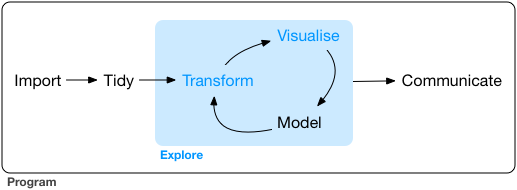
\includegraphics{img/data-science-explore.png}

The iteration loop has to be done taking the business perspective / constraint into account !

\hypertarget{resources}{%
\section{Resources}\label{resources}}

You will find a lot of resources online. Here is a selection, mostly related to R. However, our goal for this session is to have you understand how all the methods we will cover are related to each other and when you should consider using them

\begin{itemize}
\tightlist
\item
  \href{https://r4ds.had.co.nz/}{R for data science}
\item
  \href{https://www.econometrics-with-r.org/}{Statistics and econometrics}
\item
  \href{https://moderndive.com/}{Statistics and exploration with R}
\item
  \href{https://www.data-to-viz.com/}{From data to viz} (featuring python :D )
\item
  \href{https://socviz.co/}{Data visualization}
\item
  \href{https://bookdown.org/home/}{More resource online books using R (text mining, machine learning\ldots)}
\end{itemize}

\hypertarget{data-of-the-week}{%
\section{Data of the week}\label{data-of-the-week}}

In this course, we will handle with my \emph{own} personal data (I give my consent ! ;) )
Those are my sports activity data, which I got from garmin (thanks to the GDPR). If you want to get your own data from \href{https://www.garmin.com/en-US/account/datamanagement/exportdata/}{this page}.
Being a triathlete, there are several sports involved and a lot of activities. The goal will be to import, clean, analyze the data with statistics and eventually build some first models (\textbf{explainable AI}).

The export results in a lot of JSON files and we will focus on the summary data. It's real world data and you'll see it's complicated, dirty and requires a lot of preparation/manipulation !

\begin{Shaded}
\begin{Highlighting}[]
\KeywordTok{require}\NormalTok{(tidyverse)}
\NormalTok{dat <-}\StringTok{ }\KeywordTok{read.csv}\NormalTok{(}\StringTok{"Data/Sports/Activities.csv"}\NormalTok{,}\DataTypeTok{header =}\NormalTok{ T)}
\KeywordTok{head}\NormalTok{(dat)}
\end{Highlighting}
\end{Shaded}

\begin{verbatim}
##   activityId       uuidMsb       uuidLsb                name activityType
## 1 5570974040  3.695224e+18 -7.098507e+18          En piscine lap_swimming
## 2 5566524321 -5.212790e+18 -8.140623e+18     Vienna Cyclisme      cycling
## 3 5561266034  1.271356e+18 -5.522844e+18 Korneuburg Cyclisme      cycling
## 4 5555881653 -2.923938e+18 -4.676832e+18       Vienna Course      running
## 5 5551811953  7.859043e+18 -7.909532e+18      Zwift - London virtual_ride
## 6 5551052200 -9.554086e+17 -6.866435e+18          En piscine lap_swimming
##   userProfileId timeZoneId beginTimestamp eventTypeId   rule sportType
## 1       1141258        124   1.600700e+12           9 public   GENERIC
## 2       1141258        124   1.600602e+12           9 public   CYCLING
## 3       1141258        124   1.600523e+12           9 public   CYCLING
## 4       1141258        124   1.600439e+12           9 public   RUNNING
## 5       1141258        124   1.600362e+12           9 public   GENERIC
## 6       1141258        124   1.600353e+12           9 public   GENERIC
##   startTimeGmt startTimeLocal duration distance elevationGain elevationLoss
## 1 1.600700e+12   1.600708e+12  3640221   300000            NA            NA
## 2 1.600602e+12   1.600609e+12 15064570 12293220        200100        196800
## 3 1.600523e+12   1.600530e+12 10382433  8360927         74500         74200
## 4 1.600439e+12   1.600447e+12  5393830  1792890         42600         42500
## 5 1.600362e+12   1.600369e+12  3626825  3492347         16000             0
## 6 1.600353e+12   1.600360e+12  3359145   285000            NA            NA
##   avgSpeed maxSpeed avgHr maxHr  calories startLongitude startLatitude
## 1   0.0986   0.1122    NA    NA  2547.532             NA            NA
## 2   0.8160   1.9315   144   176 16345.268       16.31524      48.20915
## 3   0.8053   1.9557   117   161  8744.572       16.33986      48.34994
## 4   0.3324   1.2475   155   176  4923.274       16.31587      48.21432
## 5   0.9629   1.6364   138   163  3083.855        0.00000       0.00000
## 6   0.1011   0.3524    NA    NA  2505.632             NA            NA
##   aerobicTrainingEffect avgFractionalCadence maxFractionalCadence
## 1                    NA               0.0000                    0
## 2                   3.5               0.0000                    0
## 3                   2.4               0.0000                    0
## 4                   3.0               0.1875                    0
## 5                   0.0               0.0000                    0
## 6                    NA               0.0000                    0
##   elapsedDuration movingDuration anaerobicTrainingEffect   deviceId
## 1         3955901        3099653                      NA 3968818126
## 2        16176575       15000179                     0.0 3968818126
## 3        11319866       10356078                     0.0 3968818126
## 4         5538505        5389603                     0.2 3968818126
## 5         3629000        3611000                      NA 3825981698
## 6         3585826        2858951                      NA 3968818126
##   minTemperature maxTemperature minElevation maxElevation        locationName
## 1             25             26           NA           NA                <NA>
## 2             19             29        18480        95480              Vienna
## 3             18             29        13980        32200          Korneuburg
## 4             19             27        24920        54400              Vienna
## 5             NA             NA          300         3420 City of Westminster
## 6             26             27           NA           NA                <NA>
##   maxVerticalSpeed lapCount endLongitude endLatitude activeSets totalSets
## 1               NA       34           NA          NA         NA        NA
## 2       0.43999939       25     16.25314    48.20399         NA        NA
## 3       0.34000092       17     16.38793    48.38009         NA        NA
## 4       0.08000183       18     16.31980    48.22264         NA        NA
## 5       0.16000004        1           NA          NA         NA        NA
## 6               NA       32           NA          NA         NA        NA
##   totalReps purposeful autoCalcCalories favorite    pr elevationCorrected
## 1        NA      FALSE            FALSE    FALSE FALSE              FALSE
## 2        NA      FALSE            FALSE    FALSE FALSE              FALSE
## 3        NA      FALSE            FALSE    FALSE FALSE              FALSE
## 4        NA      FALSE            FALSE    FALSE FALSE              FALSE
## 5        NA      FALSE            FALSE    FALSE FALSE              FALSE
## 6        NA      FALSE            FALSE    FALSE FALSE              FALSE
##   atpActivity parent maxRunCadence steps avgVerticalOscillation
## 1       FALSE  FALSE            NA    NA                     NA
## 2       FALSE  FALSE            NA    NA                     NA
## 3       FALSE  FALSE            NA    NA                     NA
## 4       FALSE  FALSE           104 15620                     NA
## 5       FALSE  FALSE            NA    NA                     NA
## 6       FALSE  FALSE            NA    NA                     NA
##   avgGroundContactTime avgStrideLength vO2MaxValue avgVerticalRatio
## 1                   NA              NA          NA               NA
## 2                   NA              NA          72               NA
## 3                   NA              NA          71               NA
## 4                   NA        115.6389          58               NA
## 5                   NA              NA          NA               NA
## 6                   NA              NA          NA               NA
##   avgGroundContactBalance avgDoubleCadence maxDoubleCadence avgPower
## 1                      NA               NA               NA       NA
## 2                      NA               NA               NA      260
## 3                      NA               NA               NA      202
## 4                      NA          172.375              208       NA
## 5                      NA               NA               NA      212
## 6                      NA               NA               NA       NA
##   avgBikeCadence maxBikeCadence strokes normPower avgLeftBalance
## 1             NA             NA    1198        NA             NA
## 2             83            114   17968  296.0000          49.92
## 3             82            107   12571  231.0000          49.90
## 4             NA             NA      NA        NA             NA
## 5             91            114       0  218.3049             NA
## 6             NA             NA    1152        NA             NA
##   avgRightBalance max20MinPower trainingStressScore intensityFactor
## 1              NA            NA                  NA              NA
## 2           50.08      375.1583               291.4           0.835
## 3           50.10      242.7692               122.8           0.653
## 4              NA            NA                  NA              NA
## 5              NA      221.0525                  NA              NA
## 6              NA            NA                  NA              NA
##   lactateThresholdBpm lactateThresholdSpeed avgStrokes activeLengths avgSwolf
## 1                  NA                    NA       23.0            60       74
## 2                  NA                    NA         NA            NA       NA
## 3                  NA                    NA         NA            NA       NA
## 4                  NA                    NA         NA            NA       NA
## 5                  NA                    NA         NA            NA       NA
## 6                  NA                    NA       22.6            57       72
##   poolLength avgStrokeDistance avgSwimCadence maxSwimCadence maxFtp workoutId
## 1       5000               217             27             29     NA        NA
## 2         NA                NA             NA             NA     NA        NA
## 3         NA                NA             NA             NA     NA        NA
## 4         NA                NA             NA             NA     NA        NA
## 5         NA                NA             NA             NA     NA        NA
## 6       5000               221             27             30     NA        NA
##   decoDive parentId avgVerticalSpeed maxDepth avgDepth surfaceInterval
## 1       NA       NA               NA       NA       NA              NA
## 2       NA       NA               NA       NA       NA              NA
## 3       NA       NA               NA       NA       NA              NA
## 4       NA       NA               NA       NA       NA              NA
## 5       NA       NA               NA       NA       NA              NA
## 6       NA       NA               NA       NA       NA              NA
##   floorsDescended bottomTime
## 1              NA         NA
## 2              NA         NA
## 3              NA         NA
## 4              NA         NA
## 5              NA         NA
## 6              NA         NA
\end{verbatim}

\hypertarget{intro_r}{%
\chapter{Introduction to R}\label{intro_r}}

R is one of the most popular data science language along with Python and Julia

\hypertarget{what-is-r}{%
\section{What is R}\label{what-is-r}}

\hypertarget{description}{%
\subsection{Description}\label{description}}

R is an open source programming language initially dedicated to \textbf{statistics} and \textbf{data analysis}. It is the open-source version of the original S/S-plus language, developed by Bell labs a looong time ago. It was developed in the late 90's. Being open-source, the number of \textbf{packages} available is considerable, generating both completeness and confusion.

R is a functional programming language, meaning that \textbf{functions} are at the very core of its usage. It is not a object-oriented language although there are classes, but which are mainly hidden from the end-user.

THe basic R is a command line interface, pretty similar to the bash

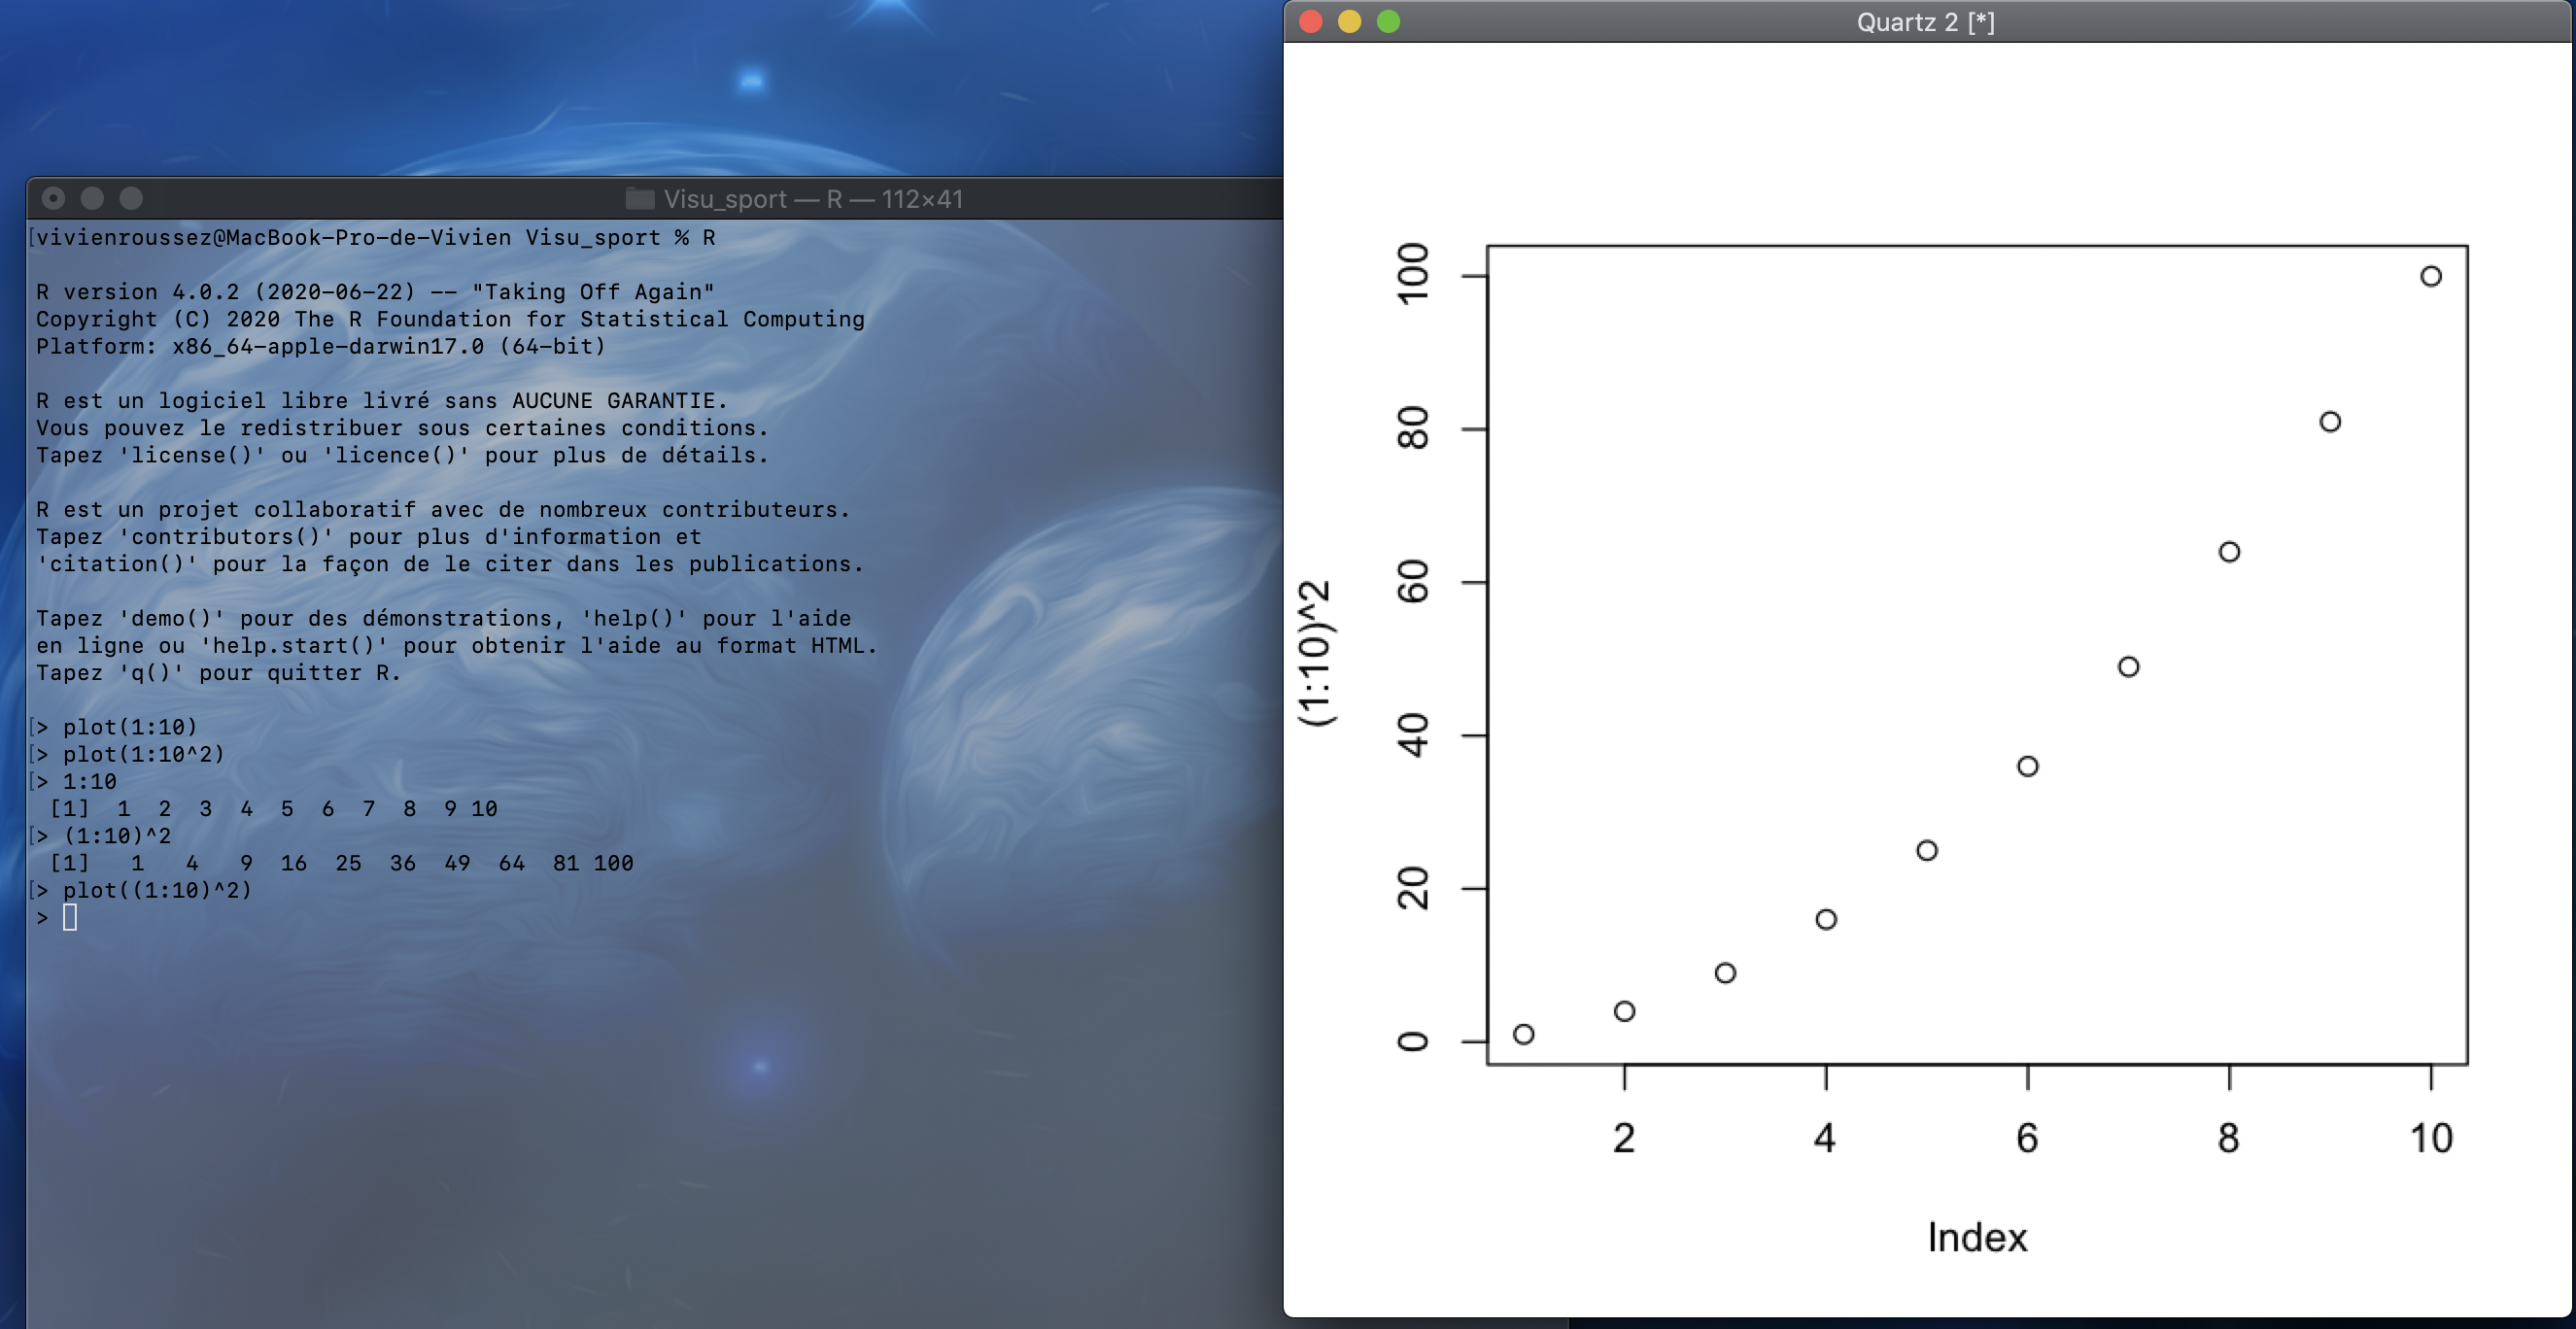
\includegraphics{img/r-console.png}
It is an \textbf{interactive} language, meaning you can execute commands one after the other, no compilation is needed to execute a sequence of commands and you can try / adjust yourt code on the fly \(\rightarrow\) very flexible (like IPython)
Another very interesting characteristic of the language is that it is by design \textbf{vectorized}, meaning operations are executed at once on vectors, without explicit loops, which makes it very effective (as long as you don't loop\ldots)

\hypertarget{objective-comparison-with-pyhton}{%
\subsection{(Objective) comparison with Pyhton}\label{objective-comparison-with-pyhton}}

What they have in common :

\begin{itemize}
\tightlist
\item
  Both language are open source and come with a wide set of capabilities and a community
\item
  Interactivity
\item
  Data science development environment (Jupyter)
\item
  Several ways to achieve the same task
\end{itemize}

What differs :

\begin{itemize}
\tightlist
\item
  R is dedicated to data / python is a generic programming language
\item
  Functional vs object oriented
\item
  Analysis (R) vs final product (Py) orientation
\end{itemize}

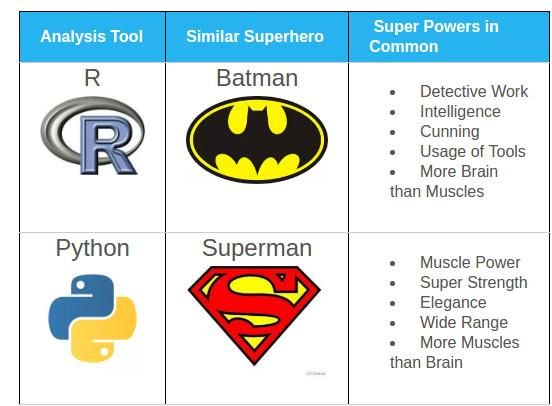
\includegraphics{img/R-python.jpg}

\hypertarget{what-can-i-do-with-r}{%
\subsection{What can I do with R}\label{what-can-i-do-with-r}}

R's core relies in data manipulation and statistical analysis. But the community made it grow in many directions

\begin{itemize}
\tightlist
\item
  Read data from multiple sources (excel, text files, databases, big data infrastructures\ldots)
\item
  \href{https://rviews.rstudio.com/2019/06/19/a-gentle-intro-to-tidymodels/}{Machine learning} and \href{https://keras.rstudio.com/}{deep learning}
\item
  \href{https://www.r-graph-gallery.com/}{Data visualization}
\item
  \href{https://shiny.rstudio.com/gallery/}{Communication}
\item
  \href{https://bookdown.org/home/}{Publications}
\item
  \ldots{} Usages I probably have no idea about !!
\end{itemize}

\hypertarget{quick-presentation-of-the-ecosystem}{%
\subsection{Quick presentation of the ecosystem}\label{quick-presentation-of-the-ecosystem}}

The core functionalities are available with base R on \href{https://cran.r-project.org/}{CRAN}. On top of that, you can install several IDEs, the most popular ones being \href{https://rstudio.com/}{Rstudio}, \href{https://jupyter.org/}{jupyter} or \href{https://code.visualstudio.com/}{VSCode}

For this training, we will use the \href{https://code.visualstudio.com/}{R kernel} of google collabs, but for many purposes, you'll have to use another IDE (shiny, markdown\ldots). This kernel comes with basics packages AND the \textbf{tidyverse}

To add features to R, you'll have then to install \href{https://cran.r-project.org/}{\textbf{packages}}. Generally, when facing a problem (eg : I have to implement a naive Bayes estimator), you google it adding r at the beginning of the query and you'll get the name of the packages that allow you to do that. Then you can install and activate it.

\begin{Shaded}
\begin{Highlighting}[]
\CommentTok{# install.packages("e1071")}
\KeywordTok{library}\NormalTok{(e1071)}
\end{Highlighting}
\end{Shaded}

\textbf{Note :} You can also call functions from an installed package without loading the whole package with \texttt{::}. You might prefer this solution in several cases :

\begin{itemize}
\tightlist
\item
  You use only one function from the package only once \(\rightarrow\) maybe not necessary to load everything
\item
  Function names can be common across packages (eg: \texttt{intersect}, \texttt{summarise}\ldots) using \texttt{::} ensures you are using the function from the package you meant.
\item
  Drawback : when not appearing at the beginning of the script, it can be unseen (for a new user) that the script requires such package to be installed
\end{itemize}

\begin{Shaded}
\begin{Highlighting}[]
\NormalTok{dplyr}\OperatorTok{::}\KeywordTok{summarise}\NormalTok{(iris,}\DataTypeTok{n_species=}\NormalTok{dplyr}\OperatorTok{::}\KeywordTok{n_distinct}\NormalTok{(Species))}
\end{Highlighting}
\end{Shaded}

\begin{verbatim}
##   n_species
## 1         3
\end{verbatim}

To find more information about R and its functinalities / latest news :

\begin{itemize}
\tightlist
\item
  \href{https://www.r-bloggers.com/}{R bloggers}
\item
  \url{tidyverse.org}
\item
  twitter : \#rstat
\item
  \href{https://rstudio.com/}{Rstudio website}
\end{itemize}

Now you can use all functions of this packages !

\hypertarget{basic-commands-to-know}{%
\section{Basic commands to know}\label{basic-commands-to-know}}

\begin{itemize}
\tightlist
\item
  Where to find help :

  \begin{itemize}
  \tightlist
  \item
    Search engine to know how to do something
  \item
    \texttt{help(lm)} or \texttt{?lm} to get help about a specific function (its inputs and output)
  \item
    stackoverflow to debug
  \end{itemize}
\item
  List the objects in memory \texttt{ls()}
\item
  What is the current directory \texttt{getwd()} ; change it \texttt{setwd()}
\item
  Browse folders and files \texttt{dir()}
\item
  Session information (loaded packages and so on) \texttt{sessionInfo()}
\item
  Install and load packages : see above
\item
  View the source code of a function : \texttt{lm}
\item
  Create a new object and assign a value to it \texttt{\textless{}-}. display in the console by typing its name
\item
  Commented lines, like in Python, start with a \texttt{\#}
\end{itemize}

\begin{Shaded}
\begin{Highlighting}[]
\NormalTok{?lm}
\KeywordTok{ls}\NormalTok{()}
\end{Highlighting}
\end{Shaded}

\begin{verbatim}
## [1] "dat"
\end{verbatim}

\begin{Shaded}
\begin{Highlighting}[]
\KeywordTok{sessionInfo}\NormalTok{()}
\end{Highlighting}
\end{Shaded}

\begin{verbatim}
## R version 4.0.2 (2020-06-22)
## Platform: x86_64-apple-darwin17.0 (64-bit)
## Running under: macOS Catalina 10.15.6
## 
## Matrix products: default
## BLAS:   /Library/Frameworks/R.framework/Versions/4.0/Resources/lib/libRblas.dylib
## LAPACK: /Library/Frameworks/R.framework/Versions/4.0/Resources/lib/libRlapack.dylib
## 
## locale:
## [1] en_US.UTF-8/en_US.UTF-8/en_US.UTF-8/C/en_US.UTF-8/en_US.UTF-8
## 
## attached base packages:
## [1] stats     graphics  grDevices utils     datasets  methods   base     
## 
## other attached packages:
##  [1] e1071_1.7-3     forcats_0.5.0   stringr_1.4.0   dplyr_1.0.2    
##  [5] purrr_0.3.4     readr_1.3.1     tidyr_1.1.2     tibble_3.0.3   
##  [9] ggplot2_3.3.2   tidyverse_1.3.0
## 
## loaded via a namespace (and not attached):
##  [1] tidyselect_1.1.0 xfun_0.17        haven_2.3.1      colorspace_1.4-1
##  [5] vctrs_0.3.4      generics_0.0.2   htmltools_0.5.0  yaml_2.2.1      
##  [9] blob_1.2.1       rlang_0.4.7      pillar_1.4.6     glue_1.4.2      
## [13] withr_2.2.0      DBI_1.1.0        dbplyr_1.4.4     modelr_0.1.8    
## [17] readxl_1.3.1     lifecycle_0.2.0  munsell_0.5.0    gtable_0.3.0    
## [21] cellranger_1.1.0 rvest_0.3.6      evaluate_0.14    knitr_1.29      
## [25] class_7.3-17     fansi_0.4.1      broom_0.7.0      Rcpp_1.0.5      
## [29] scales_1.1.1     backports_1.1.10 jsonlite_1.7.1   fs_1.5.0        
## [33] hms_0.5.3        digest_0.6.25    stringi_1.5.3    bookdown_0.20   
## [37] grid_4.0.2       cli_2.0.2        tools_4.0.2      magrittr_1.5    
## [41] crayon_1.3.4     pkgconfig_2.0.3  ellipsis_0.3.1   xml2_1.3.2      
## [45] reprex_0.3.0     lubridate_1.7.9  assertthat_0.2.1 rmarkdown_2.3   
## [49] httr_1.4.2       rstudioapi_0.11  R6_2.4.1         compiler_4.0.2
\end{verbatim}

\begin{Shaded}
\begin{Highlighting}[]
\KeywordTok{getwd}\NormalTok{()}
\end{Highlighting}
\end{Shaded}

\begin{verbatim}
## [1] "/Users/vivienroussez/Documents/Datascience/Asigmo/DataExploration"
\end{verbatim}

\begin{Shaded}
\begin{Highlighting}[]
\KeywordTok{dir}\NormalTok{(}\StringTok{"/"}\NormalTok{)}
\end{Highlighting}
\end{Shaded}

\begin{verbatim}
##  [1] "Applications" "bin"          "cores"        "dev"          "etc"         
##  [6] "home"         "Library"      "opt"          "private"      "sbin"        
## [11] "System"       "tmp"          "Users"        "usr"          "var"         
## [16] "Volumes"
\end{verbatim}

\begin{Shaded}
\begin{Highlighting}[]
\NormalTok{lm}
\end{Highlighting}
\end{Shaded}

\begin{verbatim}
## function (formula, data, subset, weights, na.action, method = "qr", 
##     model = TRUE, x = FALSE, y = FALSE, qr = TRUE, singular.ok = TRUE, 
##     contrasts = NULL, offset, ...) 
## {
##     ret.x <- x
##     ret.y <- y
##     cl <- match.call()
##     mf <- match.call(expand.dots = FALSE)
##     m <- match(c("formula", "data", "subset", "weights", "na.action", 
##         "offset"), names(mf), 0L)
##     mf <- mf[c(1L, m)]
##     mf$drop.unused.levels <- TRUE
##     mf[[1L]] <- quote(stats::model.frame)
##     mf <- eval(mf, parent.frame())
##     if (method == "model.frame") 
##         return(mf)
##     else if (method != "qr") 
##         warning(gettextf("method = '%s' is not supported. Using 'qr'", 
##             method), domain = NA)
##     mt <- attr(mf, "terms")
##     y <- model.response(mf, "numeric")
##     w <- as.vector(model.weights(mf))
##     if (!is.null(w) && !is.numeric(w)) 
##         stop("'weights' must be a numeric vector")
##     offset <- model.offset(mf)
##     mlm <- is.matrix(y)
##     ny <- if (mlm) 
##         nrow(y)
##     else length(y)
##     if (!is.null(offset)) {
##         if (!mlm) 
##             offset <- as.vector(offset)
##         if (NROW(offset) != ny) 
##             stop(gettextf("number of offsets is %d, should equal %d (number of observations)", 
##                 NROW(offset), ny), domain = NA)
##     }
##     if (is.empty.model(mt)) {
##         x <- NULL
##         z <- list(coefficients = if (mlm) matrix(NA_real_, 0, 
##             ncol(y)) else numeric(), residuals = y, fitted.values = 0 * 
##             y, weights = w, rank = 0L, df.residual = if (!is.null(w)) sum(w != 
##             0) else ny)
##         if (!is.null(offset)) {
##             z$fitted.values <- offset
##             z$residuals <- y - offset
##         }
##     }
##     else {
##         x <- model.matrix(mt, mf, contrasts)
##         z <- if (is.null(w)) 
##             lm.fit(x, y, offset = offset, singular.ok = singular.ok, 
##                 ...)
##         else lm.wfit(x, y, w, offset = offset, singular.ok = singular.ok, 
##             ...)
##     }
##     class(z) <- c(if (mlm) "mlm", "lm")
##     z$na.action <- attr(mf, "na.action")
##     z$offset <- offset
##     z$contrasts <- attr(x, "contrasts")
##     z$xlevels <- .getXlevels(mt, mf)
##     z$call <- cl
##     z$terms <- mt
##     if (model) 
##         z$model <- mf
##     if (ret.x) 
##         z$x <- x
##     if (ret.y) 
##         z$y <- y
##     if (!qr) 
##         z$qr <- NULL
##     z
## }
## <bytecode: 0x7f86369af408>
## <environment: namespace:stats>
\end{verbatim}

\begin{Shaded}
\begin{Highlighting}[]
\NormalTok{obj <-}\StringTok{ }\DecValTok{3}
\NormalTok{obj}
\end{Highlighting}
\end{Shaded}

\begin{verbatim}
## [1] 3
\end{verbatim}

\hypertarget{data-structures-in-r}{%
\section{Data structures in R}\label{data-structures-in-r}}

As mentioned, R is a \emph{functional} programming language, which means that you will always call\ldots{} functions. And functions are defined by

\begin{itemize}
\tightlist
\item
  parameters : the inputs you have to provide the function so that it can do what it's meant for
\item
  the result : the output you get. Stricly speacking, the result of a function is unique (as opposed to procedures). Of course, depending on the \textbf{class} of the result, it may of course be composite
\end{itemize}

This chapter gives you some keys to understand and explore the results as they are provided by the functions.

\hypertarget{basic-data-structures}{%
\subsection{Basic data structures}\label{basic-data-structures}}

Before introducing the data structure, a short precision about \emph{types}. Values are stored in data structures which partially depend on their type :

\begin{itemize}
\tightlist
\item
  Logical (\texttt{TRUE} or \texttt{FALSE})
\item
  Numerical (integer, continuous or complex)
\item
  Character (strings or categories)
\end{itemize}

R recognizes the type of the value and modify it dynamically (no need to declare the type and it can e changed). To force R to coerce values to another type, you can use the functions \texttt{as.numeric}, \texttt{as.character}, \texttt{as.logical}.

Important note : \texttt{NA} stands for \emph{not available} and is common to all type when a value is \textbf{missing}. You can have other missing values though for numerical variables :

\begin{itemize}
\tightlist
\item
  \texttt{Nan} (not a mumber) eg 0/0
\item
  \texttt{Inf} (infinity) eg log(0)
\end{itemize}

Attention : \texttt{NULL} applies to objects (eg a matrix or a list) and not to values themselves

\hypertarget{vectors}{%
\subsubsection{Vectors}\label{vectors}}

Vectors are the basic data structure : it is a unidimensional collection of values \emph{having the same type}. There are a lot of ways to generate vectors :

\begin{Shaded}
\begin{Highlighting}[]
\NormalTok{my_vect <-}\StringTok{ }\KeywordTok{c}\NormalTok{(}\DecValTok{1}\NormalTok{,}\DecValTok{2}\NormalTok{,}\DecValTok{19}\NormalTok{,}\DecValTok{1}\NormalTok{) ; }\KeywordTok{print}\NormalTok{(my_vect)}
\end{Highlighting}
\end{Shaded}

\begin{verbatim}
## [1]  1  2 19  1
\end{verbatim}

\begin{Shaded}
\begin{Highlighting}[]
\NormalTok{my_vect <-}\StringTok{ }\DecValTok{1}\OperatorTok{:}\DecValTok{10}\NormalTok{ ; }\KeywordTok{print}\NormalTok{(my_vect)}
\end{Highlighting}
\end{Shaded}

\begin{verbatim}
##  [1]  1  2  3  4  5  6  7  8  9 10
\end{verbatim}

\begin{Shaded}
\begin{Highlighting}[]
\NormalTok{my_vect <-}\StringTok{ }\KeywordTok{seq}\NormalTok{(}\OperatorTok{-}\DecValTok{15}\NormalTok{,}\DecValTok{100}\NormalTok{,.}\DecValTok{1}\NormalTok{) ; }\KeywordTok{print}\NormalTok{(my_vect)}
\end{Highlighting}
\end{Shaded}

\begin{verbatim}
##    [1] -15.0 -14.9 -14.8 -14.7 -14.6 -14.5 -14.4 -14.3 -14.2 -14.1 -14.0 -13.9
##   [13] -13.8 -13.7 -13.6 -13.5 -13.4 -13.3 -13.2 -13.1 -13.0 -12.9 -12.8 -12.7
##   [25] -12.6 -12.5 -12.4 -12.3 -12.2 -12.1 -12.0 -11.9 -11.8 -11.7 -11.6 -11.5
##   [37] -11.4 -11.3 -11.2 -11.1 -11.0 -10.9 -10.8 -10.7 -10.6 -10.5 -10.4 -10.3
##   [49] -10.2 -10.1 -10.0  -9.9  -9.8  -9.7  -9.6  -9.5  -9.4  -9.3  -9.2  -9.1
##   [61]  -9.0  -8.9  -8.8  -8.7  -8.6  -8.5  -8.4  -8.3  -8.2  -8.1  -8.0  -7.9
##   [73]  -7.8  -7.7  -7.6  -7.5  -7.4  -7.3  -7.2  -7.1  -7.0  -6.9  -6.8  -6.7
##   [85]  -6.6  -6.5  -6.4  -6.3  -6.2  -6.1  -6.0  -5.9  -5.8  -5.7  -5.6  -5.5
##   [97]  -5.4  -5.3  -5.2  -5.1  -5.0  -4.9  -4.8  -4.7  -4.6  -4.5  -4.4  -4.3
##  [109]  -4.2  -4.1  -4.0  -3.9  -3.8  -3.7  -3.6  -3.5  -3.4  -3.3  -3.2  -3.1
##  [121]  -3.0  -2.9  -2.8  -2.7  -2.6  -2.5  -2.4  -2.3  -2.2  -2.1  -2.0  -1.9
##  [133]  -1.8  -1.7  -1.6  -1.5  -1.4  -1.3  -1.2  -1.1  -1.0  -0.9  -0.8  -0.7
##  [145]  -0.6  -0.5  -0.4  -0.3  -0.2  -0.1   0.0   0.1   0.2   0.3   0.4   0.5
##  [157]   0.6   0.7   0.8   0.9   1.0   1.1   1.2   1.3   1.4   1.5   1.6   1.7
##  [169]   1.8   1.9   2.0   2.1   2.2   2.3   2.4   2.5   2.6   2.7   2.8   2.9
##  [181]   3.0   3.1   3.2   3.3   3.4   3.5   3.6   3.7   3.8   3.9   4.0   4.1
##  [193]   4.2   4.3   4.4   4.5   4.6   4.7   4.8   4.9   5.0   5.1   5.2   5.3
##  [205]   5.4   5.5   5.6   5.7   5.8   5.9   6.0   6.1   6.2   6.3   6.4   6.5
##  [217]   6.6   6.7   6.8   6.9   7.0   7.1   7.2   7.3   7.4   7.5   7.6   7.7
##  [229]   7.8   7.9   8.0   8.1   8.2   8.3   8.4   8.5   8.6   8.7   8.8   8.9
##  [241]   9.0   9.1   9.2   9.3   9.4   9.5   9.6   9.7   9.8   9.9  10.0  10.1
##  [253]  10.2  10.3  10.4  10.5  10.6  10.7  10.8  10.9  11.0  11.1  11.2  11.3
##  [265]  11.4  11.5  11.6  11.7  11.8  11.9  12.0  12.1  12.2  12.3  12.4  12.5
##  [277]  12.6  12.7  12.8  12.9  13.0  13.1  13.2  13.3  13.4  13.5  13.6  13.7
##  [289]  13.8  13.9  14.0  14.1  14.2  14.3  14.4  14.5  14.6  14.7  14.8  14.9
##  [301]  15.0  15.1  15.2  15.3  15.4  15.5  15.6  15.7  15.8  15.9  16.0  16.1
##  [313]  16.2  16.3  16.4  16.5  16.6  16.7  16.8  16.9  17.0  17.1  17.2  17.3
##  [325]  17.4  17.5  17.6  17.7  17.8  17.9  18.0  18.1  18.2  18.3  18.4  18.5
##  [337]  18.6  18.7  18.8  18.9  19.0  19.1  19.2  19.3  19.4  19.5  19.6  19.7
##  [349]  19.8  19.9  20.0  20.1  20.2  20.3  20.4  20.5  20.6  20.7  20.8  20.9
##  [361]  21.0  21.1  21.2  21.3  21.4  21.5  21.6  21.7  21.8  21.9  22.0  22.1
##  [373]  22.2  22.3  22.4  22.5  22.6  22.7  22.8  22.9  23.0  23.1  23.2  23.3
##  [385]  23.4  23.5  23.6  23.7  23.8  23.9  24.0  24.1  24.2  24.3  24.4  24.5
##  [397]  24.6  24.7  24.8  24.9  25.0  25.1  25.2  25.3  25.4  25.5  25.6  25.7
##  [409]  25.8  25.9  26.0  26.1  26.2  26.3  26.4  26.5  26.6  26.7  26.8  26.9
##  [421]  27.0  27.1  27.2  27.3  27.4  27.5  27.6  27.7  27.8  27.9  28.0  28.1
##  [433]  28.2  28.3  28.4  28.5  28.6  28.7  28.8  28.9  29.0  29.1  29.2  29.3
##  [445]  29.4  29.5  29.6  29.7  29.8  29.9  30.0  30.1  30.2  30.3  30.4  30.5
##  [457]  30.6  30.7  30.8  30.9  31.0  31.1  31.2  31.3  31.4  31.5  31.6  31.7
##  [469]  31.8  31.9  32.0  32.1  32.2  32.3  32.4  32.5  32.6  32.7  32.8  32.9
##  [481]  33.0  33.1  33.2  33.3  33.4  33.5  33.6  33.7  33.8  33.9  34.0  34.1
##  [493]  34.2  34.3  34.4  34.5  34.6  34.7  34.8  34.9  35.0  35.1  35.2  35.3
##  [505]  35.4  35.5  35.6  35.7  35.8  35.9  36.0  36.1  36.2  36.3  36.4  36.5
##  [517]  36.6  36.7  36.8  36.9  37.0  37.1  37.2  37.3  37.4  37.5  37.6  37.7
##  [529]  37.8  37.9  38.0  38.1  38.2  38.3  38.4  38.5  38.6  38.7  38.8  38.9
##  [541]  39.0  39.1  39.2  39.3  39.4  39.5  39.6  39.7  39.8  39.9  40.0  40.1
##  [553]  40.2  40.3  40.4  40.5  40.6  40.7  40.8  40.9  41.0  41.1  41.2  41.3
##  [565]  41.4  41.5  41.6  41.7  41.8  41.9  42.0  42.1  42.2  42.3  42.4  42.5
##  [577]  42.6  42.7  42.8  42.9  43.0  43.1  43.2  43.3  43.4  43.5  43.6  43.7
##  [589]  43.8  43.9  44.0  44.1  44.2  44.3  44.4  44.5  44.6  44.7  44.8  44.9
##  [601]  45.0  45.1  45.2  45.3  45.4  45.5  45.6  45.7  45.8  45.9  46.0  46.1
##  [613]  46.2  46.3  46.4  46.5  46.6  46.7  46.8  46.9  47.0  47.1  47.2  47.3
##  [625]  47.4  47.5  47.6  47.7  47.8  47.9  48.0  48.1  48.2  48.3  48.4  48.5
##  [637]  48.6  48.7  48.8  48.9  49.0  49.1  49.2  49.3  49.4  49.5  49.6  49.7
##  [649]  49.8  49.9  50.0  50.1  50.2  50.3  50.4  50.5  50.6  50.7  50.8  50.9
##  [661]  51.0  51.1  51.2  51.3  51.4  51.5  51.6  51.7  51.8  51.9  52.0  52.1
##  [673]  52.2  52.3  52.4  52.5  52.6  52.7  52.8  52.9  53.0  53.1  53.2  53.3
##  [685]  53.4  53.5  53.6  53.7  53.8  53.9  54.0  54.1  54.2  54.3  54.4  54.5
##  [697]  54.6  54.7  54.8  54.9  55.0  55.1  55.2  55.3  55.4  55.5  55.6  55.7
##  [709]  55.8  55.9  56.0  56.1  56.2  56.3  56.4  56.5  56.6  56.7  56.8  56.9
##  [721]  57.0  57.1  57.2  57.3  57.4  57.5  57.6  57.7  57.8  57.9  58.0  58.1
##  [733]  58.2  58.3  58.4  58.5  58.6  58.7  58.8  58.9  59.0  59.1  59.2  59.3
##  [745]  59.4  59.5  59.6  59.7  59.8  59.9  60.0  60.1  60.2  60.3  60.4  60.5
##  [757]  60.6  60.7  60.8  60.9  61.0  61.1  61.2  61.3  61.4  61.5  61.6  61.7
##  [769]  61.8  61.9  62.0  62.1  62.2  62.3  62.4  62.5  62.6  62.7  62.8  62.9
##  [781]  63.0  63.1  63.2  63.3  63.4  63.5  63.6  63.7  63.8  63.9  64.0  64.1
##  [793]  64.2  64.3  64.4  64.5  64.6  64.7  64.8  64.9  65.0  65.1  65.2  65.3
##  [805]  65.4  65.5  65.6  65.7  65.8  65.9  66.0  66.1  66.2  66.3  66.4  66.5
##  [817]  66.6  66.7  66.8  66.9  67.0  67.1  67.2  67.3  67.4  67.5  67.6  67.7
##  [829]  67.8  67.9  68.0  68.1  68.2  68.3  68.4  68.5  68.6  68.7  68.8  68.9
##  [841]  69.0  69.1  69.2  69.3  69.4  69.5  69.6  69.7  69.8  69.9  70.0  70.1
##  [853]  70.2  70.3  70.4  70.5  70.6  70.7  70.8  70.9  71.0  71.1  71.2  71.3
##  [865]  71.4  71.5  71.6  71.7  71.8  71.9  72.0  72.1  72.2  72.3  72.4  72.5
##  [877]  72.6  72.7  72.8  72.9  73.0  73.1  73.2  73.3  73.4  73.5  73.6  73.7
##  [889]  73.8  73.9  74.0  74.1  74.2  74.3  74.4  74.5  74.6  74.7  74.8  74.9
##  [901]  75.0  75.1  75.2  75.3  75.4  75.5  75.6  75.7  75.8  75.9  76.0  76.1
##  [913]  76.2  76.3  76.4  76.5  76.6  76.7  76.8  76.9  77.0  77.1  77.2  77.3
##  [925]  77.4  77.5  77.6  77.7  77.8  77.9  78.0  78.1  78.2  78.3  78.4  78.5
##  [937]  78.6  78.7  78.8  78.9  79.0  79.1  79.2  79.3  79.4  79.5  79.6  79.7
##  [949]  79.8  79.9  80.0  80.1  80.2  80.3  80.4  80.5  80.6  80.7  80.8  80.9
##  [961]  81.0  81.1  81.2  81.3  81.4  81.5  81.6  81.7  81.8  81.9  82.0  82.1
##  [973]  82.2  82.3  82.4  82.5  82.6  82.7  82.8  82.9  83.0  83.1  83.2  83.3
##  [985]  83.4  83.5  83.6  83.7  83.8  83.9  84.0  84.1  84.2  84.3  84.4  84.5
##  [997]  84.6  84.7  84.8  84.9  85.0  85.1  85.2  85.3  85.4  85.5  85.6  85.7
## [1009]  85.8  85.9  86.0  86.1  86.2  86.3  86.4  86.5  86.6  86.7  86.8  86.9
## [1021]  87.0  87.1  87.2  87.3  87.4  87.5  87.6  87.7  87.8  87.9  88.0  88.1
## [1033]  88.2  88.3  88.4  88.5  88.6  88.7  88.8  88.9  89.0  89.1  89.2  89.3
## [1045]  89.4  89.5  89.6  89.7  89.8  89.9  90.0  90.1  90.2  90.3  90.4  90.5
## [1057]  90.6  90.7  90.8  90.9  91.0  91.1  91.2  91.3  91.4  91.5  91.6  91.7
## [1069]  91.8  91.9  92.0  92.1  92.2  92.3  92.4  92.5  92.6  92.7  92.8  92.9
## [1081]  93.0  93.1  93.2  93.3  93.4  93.5  93.6  93.7  93.8  93.9  94.0  94.1
## [1093]  94.2  94.3  94.4  94.5  94.6  94.7  94.8  94.9  95.0  95.1  95.2  95.3
## [1105]  95.4  95.5  95.6  95.7  95.8  95.9  96.0  96.1  96.2  96.3  96.4  96.5
## [1117]  96.6  96.7  96.8  96.9  97.0  97.1  97.2  97.3  97.4  97.5  97.6  97.7
## [1129]  97.8  97.9  98.0  98.1  98.2  98.3  98.4  98.5  98.6  98.7  98.8  98.9
## [1141]  99.0  99.1  99.2  99.3  99.4  99.5  99.6  99.7  99.8  99.9 100.0
\end{verbatim}

\begin{Shaded}
\begin{Highlighting}[]
\NormalTok{my_vect <-}\StringTok{ }\KeywordTok{rnorm}\NormalTok{(}\DecValTok{100}\NormalTok{) ; }\KeywordTok{print}\NormalTok{(my_vect)}
\end{Highlighting}
\end{Shaded}

\begin{verbatim}
##   [1] -1.21004842 -1.06121248  0.71634673  1.47637602  0.48728132 -1.40233045
##   [7] -0.01020396 -1.00491601 -1.13058465 -0.51105332 -3.04697783 -0.41697855
##  [13]  1.14776250 -0.06190428 -0.61406102  1.08143552  2.37724254  2.27646272
##  [19]  0.91724004 -0.44129808  0.03188855 -0.89633876  0.18671548 -0.23189549
##  [25]  1.67617991 -0.27757116  0.26018862  2.00163360 -1.41111960 -0.55119739
##  [31]  1.42648442  0.73438772  0.86664661 -0.89074131  0.32450045  0.86402894
##  [37] -1.85744581  0.82117312  0.20926134 -1.02316778 -0.69767865 -0.77886117
##  [43] -0.42240714  0.41656734  0.51914181 -0.20057167  0.19494615  0.01393820
##  [49] -0.99481747  0.54007011  0.49309055 -0.79606589 -2.36025571  0.48564480
##  [55]  0.29072507 -0.38146633  0.56337763 -0.48490022  1.06052814  0.24571570
##  [61]  0.46890216 -0.24452292 -0.92088724 -0.86546828 -0.18666685  0.78926829
##  [67] -0.78086945  0.46444770 -0.76284691  0.61650581  0.59103079 -0.17137042
##  [73]  0.12108668 -1.63122288 -0.80778850  1.06061406 -0.95744478  0.36101337
##  [79]  0.05042920 -0.97059999 -1.80390869  0.15294386  0.32179016  1.11523338
##  [85]  0.33365395 -1.17738912  1.46300597 -0.29402040 -0.06691599 -0.45963294
##  [91]  0.46536078  1.06914660 -1.00272811 -1.26934158 -0.55375181 -0.09793410
##  [97] -2.65666912 -0.76039332  0.33721873 -0.39925402
\end{verbatim}

\begin{Shaded}
\begin{Highlighting}[]
\NormalTok{my_vect <-}\StringTok{ }\KeywordTok{sample}\NormalTok{(letters,}\DecValTok{100}\NormalTok{,}\DataTypeTok{replace =}\NormalTok{ T) ; }\KeywordTok{print}\NormalTok{(my_vect)}
\end{Highlighting}
\end{Shaded}

\begin{verbatim}
##   [1] "u" "x" "a" "g" "m" "f" "a" "y" "p" "i" "n" "r" "i" "m" "d" "u" "c" "v"
##  [19] "p" "k" "e" "d" "f" "n" "i" "h" "d" "h" "z" "f" "t" "s" "g" "t" "b" "m"
##  [37] "a" "f" "a" "s" "z" "c" "u" "g" "s" "t" "t" "l" "g" "j" "g" "i" "v" "o"
##  [55] "k" "n" "l" "l" "k" "d" "t" "m" "v" "p" "t" "z" "q" "t" "o" "d" "v" "j"
##  [73] "l" "t" "h" "u" "m" "f" "q" "b" "c" "q" "s" "w" "j" "j" "s" "m" "o" "z"
##  [91] "h" "n" "y" "d" "w" "f" "r" "z" "h" "e"
\end{verbatim}

You can access vector values with integer indexes (that are vector themselves). \textbf{Note :} unlike Python, the indexes start with the value 1, not 0 !

\begin{Shaded}
\begin{Highlighting}[]
\NormalTok{my_vect[}\DecValTok{4}\NormalTok{]}
\end{Highlighting}
\end{Shaded}

\begin{verbatim}
## [1] "g"
\end{verbatim}

\begin{Shaded}
\begin{Highlighting}[]
\NormalTok{my_vect[}\DecValTok{1}\OperatorTok{:}\DecValTok{4}\NormalTok{]}
\end{Highlighting}
\end{Shaded}

\begin{verbatim}
## [1] "u" "x" "a" "g"
\end{verbatim}

A vector can be \emph{named} meaning that each element has a name through which it can be accessed.

\begin{Shaded}
\begin{Highlighting}[]
\NormalTok{my_vect <-}\StringTok{ }\DecValTok{1}\OperatorTok{:}\DecValTok{10}
\KeywordTok{names}\NormalTok{(my_vect) <-}\StringTok{ }\NormalTok{letters[}\DecValTok{1}\OperatorTok{:}\DecValTok{10}\NormalTok{] ; }\KeywordTok{print}\NormalTok{(my_vect)}
\end{Highlighting}
\end{Shaded}

\begin{verbatim}
##  a  b  c  d  e  f  g  h  i  j 
##  1  2  3  4  5  6  7  8  9 10
\end{verbatim}

\begin{Shaded}
\begin{Highlighting}[]
\NormalTok{my_vect[}\StringTok{"b"}\NormalTok{]}
\end{Highlighting}
\end{Shaded}

\begin{verbatim}
## b 
## 2
\end{verbatim}

Did you notice you can assign values to a vector's attribute ? :D

\hypertarget{matrices-and-arrays}{%
\subsubsection{Matrices and arrays}\label{matrices-and-arrays}}

Matrices are a 2-dimensional collection of values \emph{having the same type}. An array is an extension of matrices for more than 2 dimensions.

\begin{Shaded}
\begin{Highlighting}[]
\NormalTok{mat <-}\StringTok{ }\KeywordTok{matrix}\NormalTok{(}\DecValTok{1}\NormalTok{,}\DataTypeTok{ncol=}\DecValTok{10}\NormalTok{,}\DataTypeTok{nrow =} \DecValTok{15}\NormalTok{) ; }\KeywordTok{print}\NormalTok{(mat)}
\end{Highlighting}
\end{Shaded}

\begin{verbatim}
##       [,1] [,2] [,3] [,4] [,5] [,6] [,7] [,8] [,9] [,10]
##  [1,]    1    1    1    1    1    1    1    1    1     1
##  [2,]    1    1    1    1    1    1    1    1    1     1
##  [3,]    1    1    1    1    1    1    1    1    1     1
##  [4,]    1    1    1    1    1    1    1    1    1     1
##  [5,]    1    1    1    1    1    1    1    1    1     1
##  [6,]    1    1    1    1    1    1    1    1    1     1
##  [7,]    1    1    1    1    1    1    1    1    1     1
##  [8,]    1    1    1    1    1    1    1    1    1     1
##  [9,]    1    1    1    1    1    1    1    1    1     1
## [10,]    1    1    1    1    1    1    1    1    1     1
## [11,]    1    1    1    1    1    1    1    1    1     1
## [12,]    1    1    1    1    1    1    1    1    1     1
## [13,]    1    1    1    1    1    1    1    1    1     1
## [14,]    1    1    1    1    1    1    1    1    1     1
## [15,]    1    1    1    1    1    1    1    1    1     1
\end{verbatim}

\begin{Shaded}
\begin{Highlighting}[]
\NormalTok{mat <-}\StringTok{ }\KeywordTok{matrix}\NormalTok{(}\DecValTok{1}\OperatorTok{:}\DecValTok{5}\NormalTok{,}\DataTypeTok{ncol=}\DecValTok{5}\NormalTok{,}\DataTypeTok{nrow=}\DecValTok{7}\NormalTok{) ; }\KeywordTok{print}\NormalTok{(mat)}
\end{Highlighting}
\end{Shaded}

\begin{verbatim}
##      [,1] [,2] [,3] [,4] [,5]
## [1,]    1    3    5    2    4
## [2,]    2    4    1    3    5
## [3,]    3    5    2    4    1
## [4,]    4    1    3    5    2
## [5,]    5    2    4    1    3
## [6,]    1    3    5    2    4
## [7,]    2    4    1    3    5
\end{verbatim}

\begin{Shaded}
\begin{Highlighting}[]
\NormalTok{arr <-}\StringTok{ }\KeywordTok{array}\NormalTok{(}\DecValTok{1}\OperatorTok{:}\DecValTok{10}\NormalTok{,}\DataTypeTok{dim =} \KeywordTok{c}\NormalTok{(}\DecValTok{10}\NormalTok{,}\DecValTok{2}\NormalTok{,}\DecValTok{3}\NormalTok{)) ; }\KeywordTok{print}\NormalTok{(arr)}
\end{Highlighting}
\end{Shaded}

\begin{verbatim}
## , , 1
## 
##       [,1] [,2]
##  [1,]    1    1
##  [2,]    2    2
##  [3,]    3    3
##  [4,]    4    4
##  [5,]    5    5
##  [6,]    6    6
##  [7,]    7    7
##  [8,]    8    8
##  [9,]    9    9
## [10,]   10   10
## 
## , , 2
## 
##       [,1] [,2]
##  [1,]    1    1
##  [2,]    2    2
##  [3,]    3    3
##  [4,]    4    4
##  [5,]    5    5
##  [6,]    6    6
##  [7,]    7    7
##  [8,]    8    8
##  [9,]    9    9
## [10,]   10   10
## 
## , , 3
## 
##       [,1] [,2]
##  [1,]    1    1
##  [2,]    2    2
##  [3,]    3    3
##  [4,]    4    4
##  [5,]    5    5
##  [6,]    6    6
##  [7,]    7    7
##  [8,]    8    8
##  [9,]    9    9
## [10,]   10   10
\end{verbatim}

\begin{Shaded}
\begin{Highlighting}[]
\KeywordTok{matrix}\NormalTok{(}\KeywordTok{rnorm}\NormalTok{(}\DecValTok{9}\NormalTok{),}\DecValTok{3}\NormalTok{,}\DecValTok{3}\NormalTok{)}
\NormalTok{m1 <-}\StringTok{ }\KeywordTok{matrix}\NormalTok{(}\DecValTok{1}\NormalTok{,}\DecValTok{2}\NormalTok{,}\DecValTok{3}\NormalTok{)}
\NormalTok{m2 <-}\StringTok{ }\KeywordTok{matrix}\NormalTok{(}\DecValTok{1}\NormalTok{,}\DecValTok{3}\NormalTok{,}\DecValTok{2}\NormalTok{)}
\NormalTok{m1}\OperatorTok{*}\NormalTok{m2}
\end{Highlighting}
\end{Shaded}

\hypertarget{lists}{%
\subsubsection{Lists}\label{lists}}

Lists are a very versatile and convenient class that allows you to store heterogeneous values and data structures

\begin{Shaded}
\begin{Highlighting}[]
\NormalTok{my_list <-}\StringTok{ }\KeywordTok{list}\NormalTok{(}\StringTok{"A"}\NormalTok{,}\DecValTok{1}\NormalTok{,LETTERS[}\DecValTok{1}\OperatorTok{:}\DecValTok{10}\NormalTok{],}\KeywordTok{matrix}\NormalTok{(}\DecValTok{1}\NormalTok{,}\DecValTok{3}\NormalTok{,}\DecValTok{3}\NormalTok{)) ; my_list}
\end{Highlighting}
\end{Shaded}

\begin{verbatim}
## [[1]]
## [1] "A"
## 
## [[2]]
## [1] 1
## 
## [[3]]
##  [1] "A" "B" "C" "D" "E" "F" "G" "H" "I" "J"
## 
## [[4]]
##      [,1] [,2] [,3]
## [1,]    1    1    1
## [2,]    1    1    1
## [3,]    1    1    1
\end{verbatim}

Like with vectors, list elements can be accessed via their index or their name. If a list has been named, you have something very similar to python dictionaries. In case the list is named, you can also access its elements via the \texttt{\$} operator.

\begin{Shaded}
\begin{Highlighting}[]
\KeywordTok{names}\NormalTok{(my_list) <-}\StringTok{ }\KeywordTok{paste0}\NormalTok{(}\StringTok{"thing"}\NormalTok{,}\DecValTok{1}\OperatorTok{:}\KeywordTok{length}\NormalTok{(my_list))}
\NormalTok{my_list[}\DecValTok{1}\NormalTok{]}
\end{Highlighting}
\end{Shaded}

\begin{verbatim}
## $thing1
## [1] "A"
\end{verbatim}

\begin{Shaded}
\begin{Highlighting}[]
\NormalTok{my_list[}\StringTok{"thing1"}\NormalTok{]}
\end{Highlighting}
\end{Shaded}

\begin{verbatim}
## $thing1
## [1] "A"
\end{verbatim}

\begin{Shaded}
\begin{Highlighting}[]
\NormalTok{my_list}\OperatorTok{$}\NormalTok{thing3}
\end{Highlighting}
\end{Shaded}

\begin{verbatim}
##  [1] "A" "B" "C" "D" "E" "F" "G" "H" "I" "J"
\end{verbatim}

\begin{Shaded}
\begin{Highlighting}[]
\CommentTok{# my_list[2]*10}
\end{Highlighting}
\end{Shaded}

\hypertarget{dataframes}{%
\subsubsection{Dataframes}\label{dataframes}}

A Dataframe is the most common data representation (think of an excel spreadsheet): it is made out of columns and rows like a matrix, but the columns can have different types.
In R, Dataframes are natives (no need to install another package). They are basically a list of vectors that have the same length.

Let's have a look at Fisher's iris dataframe (included in base R for demonstration purposes)

\begin{Shaded}
\begin{Highlighting}[]
\KeywordTok{head}\NormalTok{(iris)}
\end{Highlighting}
\end{Shaded}

\begin{verbatim}
##   Sepal.Length Sepal.Width Petal.Length Petal.Width Species
## 1          5.1         3.5          1.4         0.2  setosa
## 2          4.9         3.0          1.4         0.2  setosa
## 3          4.7         3.2          1.3         0.2  setosa
## 4          4.6         3.1          1.5         0.2  setosa
## 5          5.0         3.6          1.4         0.2  setosa
## 6          5.4         3.9          1.7         0.4  setosa
\end{verbatim}

to explore the content of a dataframe, you can of course print it, but if you want amore detailed overview of it, you can use the \texttt{str} or the \texttt{glimpse} functions

\begin{Shaded}
\begin{Highlighting}[]
\KeywordTok{str}\NormalTok{(iris)}
\end{Highlighting}
\end{Shaded}

\begin{verbatim}
## 'data.frame':	150 obs. of  5 variables:
##  $ Sepal.Length: num  5.1 4.9 4.7 4.6 5 5.4 4.6 5 4.4 4.9 ...
##  $ Sepal.Width : num  3.5 3 3.2 3.1 3.6 3.9 3.4 3.4 2.9 3.1 ...
##  $ Petal.Length: num  1.4 1.4 1.3 1.5 1.4 1.7 1.4 1.5 1.4 1.5 ...
##  $ Petal.Width : num  0.2 0.2 0.2 0.2 0.2 0.4 0.3 0.2 0.2 0.1 ...
##  $ Species     : Factor w/ 3 levels "setosa","versicolor",..: 1 1 1 1 1 1 1 1 1 1 ...
\end{verbatim}

\begin{Shaded}
\begin{Highlighting}[]
\KeywordTok{glimpse}\NormalTok{(iris)}
\end{Highlighting}
\end{Shaded}

\begin{verbatim}
## Rows: 150
## Columns: 5
## $ Sepal.Length <dbl> 5.1, 4.9, 4.7, 4.6, 5.0, 5.4, 4.6, 5.0, 4.4, 4.9, 5.4,...
## $ Sepal.Width  <dbl> 3.5, 3.0, 3.2, 3.1, 3.6, 3.9, 3.4, 3.4, 2.9, 3.1, 3.7,...
## $ Petal.Length <dbl> 1.4, 1.4, 1.3, 1.5, 1.4, 1.7, 1.4, 1.5, 1.4, 1.5, 1.5,...
## $ Petal.Width  <dbl> 0.2, 0.2, 0.2, 0.2, 0.2, 0.4, 0.3, 0.2, 0.2, 0.1, 0.2,...
## $ Species      <fct> setosa, setosa, setosa, setosa, setosa, setosa, setosa...
\end{verbatim}

In general, \texttt{str} (for structure) is a very powerful function to explore the content of a data structure (see next part). To explore it further, you can use the following functions

\begin{Shaded}
\begin{Highlighting}[]
\KeywordTok{names}\NormalTok{(iris)}
\end{Highlighting}
\end{Shaded}

\begin{verbatim}
## [1] "Sepal.Length" "Sepal.Width"  "Petal.Length" "Petal.Width"  "Species"
\end{verbatim}

\begin{Shaded}
\begin{Highlighting}[]
\KeywordTok{summary}\NormalTok{(iris)}
\end{Highlighting}
\end{Shaded}

\begin{verbatim}
##   Sepal.Length    Sepal.Width     Petal.Length    Petal.Width   
##  Min.   :4.300   Min.   :2.000   Min.   :1.000   Min.   :0.100  
##  1st Qu.:5.100   1st Qu.:2.800   1st Qu.:1.600   1st Qu.:0.300  
##  Median :5.800   Median :3.000   Median :4.350   Median :1.300  
##  Mean   :5.843   Mean   :3.057   Mean   :3.758   Mean   :1.199  
##  3rd Qu.:6.400   3rd Qu.:3.300   3rd Qu.:5.100   3rd Qu.:1.800  
##  Max.   :7.900   Max.   :4.400   Max.   :6.900   Max.   :2.500  
##        Species  
##  setosa    :50  
##  versicolor:50  
##  virginica :50  
##                 
##                 
## 
\end{verbatim}

\begin{Shaded}
\begin{Highlighting}[]
\KeywordTok{plot}\NormalTok{(iris) }\CommentTok{# don't do that with too big data of course !}
\end{Highlighting}
\end{Shaded}

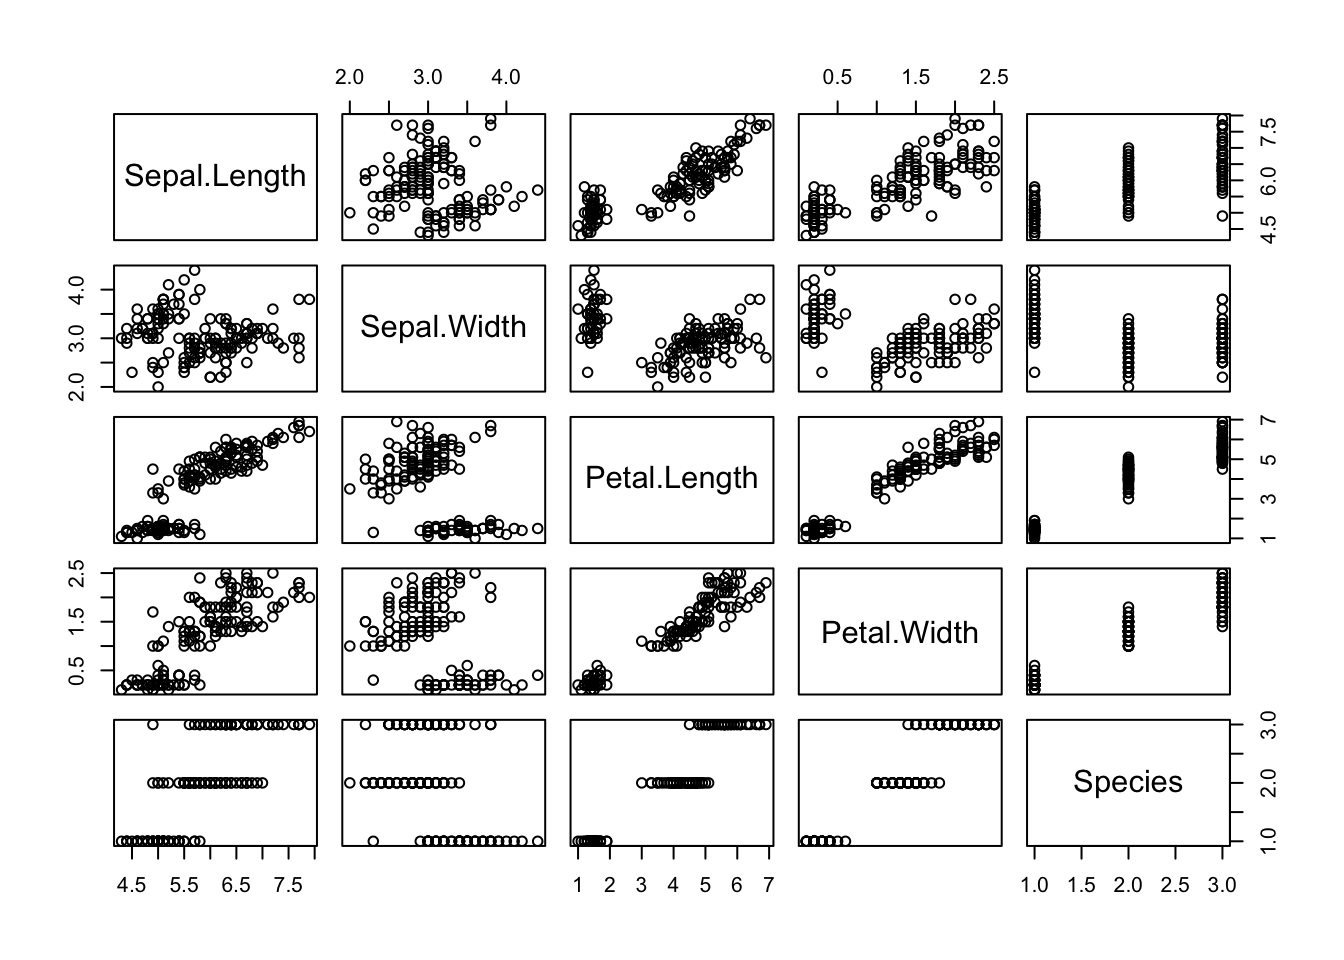
\includegraphics{DataExploration_files/figure-latex/unnamed-chunk-15-1.pdf}

\hypertarget{functions}{%
\subsubsection{Functions}\label{functions}}

As mentioned before, R is a functional programming langueage and you can of course create your own functions (which can be afterwards integrated in a package). To cfeate a function, the syntax is such :

\begin{Shaded}
\begin{Highlighting}[]
\NormalTok{square <-}\StringTok{ }\ControlFlowTok{function}\NormalTok{(}\DataTypeTok{xx=}\DecValTok{2}\NormalTok{) }\CommentTok{# 2 is the default value (not mandatory)}
\NormalTok{\{}
\NormalTok{  res <-}\StringTok{ }\NormalTok{xx}\OperatorTok{^}\DecValTok{2}
  \KeywordTok{return}\NormalTok{(res)}
\NormalTok{\}}
\CommentTok{# Shorthand}
\CommentTok{# square <- function(xx) xx^2}
\CommentTok{# Use it}
\KeywordTok{square}\NormalTok{()}
\end{Highlighting}
\end{Shaded}

\begin{verbatim}
## [1] 4
\end{verbatim}

\begin{Shaded}
\begin{Highlighting}[]
\KeywordTok{square}\NormalTok{(}\DecValTok{5}\NormalTok{)}
\end{Highlighting}
\end{Shaded}

\begin{verbatim}
## [1] 25
\end{verbatim}

\hypertarget{exercices}{%
\subsubsection{Exercices}\label{exercices}}

\begin{itemize}
\tightlist
\item
  Create a vector mixing both numbers and strings : what happens ?
\item
  Create a vector containing the values ``fellow 1'' to fellow 15". Hint : be lazy and use the \texttt{paste()} function
\item
  Replace the value ``fellow 5'' with ``best fellow''
\item
  Create a matrix (3,3) of random numbers drawn from a gaussian distribution.
\item
  Create two numerical matrices of size resp (2,3) and (3,2) filled with 1s and compute their product
\item
  From the previous list, the second element is a number ; multiply this number by 10 accessing it via its index
\item
  Create a new list containing the previous list and some other random elements
\end{itemize}

\hypertarget{explore-a-new-data-structure-or-object}{%
\subsection{Explore a new data structure (or object)}\label{explore-a-new-data-structure-or-object}}

You will often face new data structures resulting from new functions, and they will be more complicated than the ones we've just covered.

Let us take the example of the linear regression (which we will cover in section \ref{reg})

\begin{Shaded}
\begin{Highlighting}[]
\KeywordTok{library}\NormalTok{(ggplot2)}
\KeywordTok{ggplot}\NormalTok{(iris,}\KeywordTok{aes}\NormalTok{(Petal.Length,Sepal.Length)) }\OperatorTok{+}\StringTok{ }\KeywordTok{geom_jitter}\NormalTok{() }\OperatorTok{+}\StringTok{ }
\StringTok{  }\KeywordTok{geom_smooth}\NormalTok{(}\DataTypeTok{method=}\StringTok{"lm"}\NormalTok{) }\OperatorTok{+}
\StringTok{  }\KeywordTok{theme_minimal}\NormalTok{()}
\end{Highlighting}
\end{Shaded}

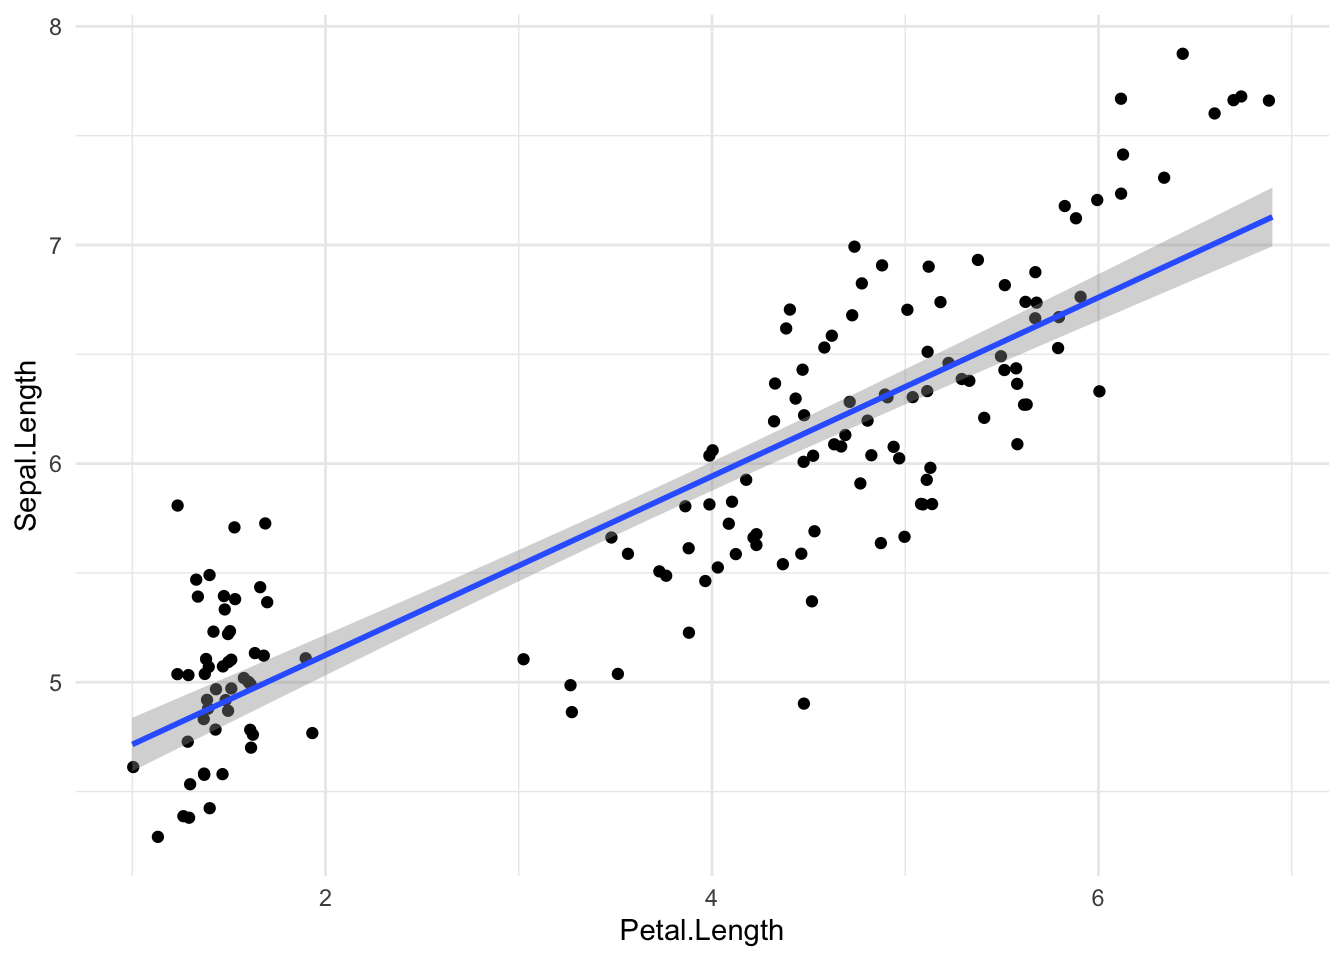
\includegraphics{DataExploration_files/figure-latex/unnamed-chunk-17-1.pdf}

\textbf{Spoiler alert :} the regression aims to find \(\alpha\) and \(\beta\) such that an explained variable \(y\) can be expressed as \(y = \alpha \cdot x + \beta\) where \(x\) is an explanatory variable. In R, to find the values of \(\alpha\) and \(\beta\), you will use the \texttt{lm}function. So let's fit this model and print the result

\begin{Shaded}
\begin{Highlighting}[]
\NormalTok{reg <-}\StringTok{ }\KeywordTok{lm}\NormalTok{(Petal.Length }\OperatorTok{~}\StringTok{ }\NormalTok{Sepal.Length,}\DataTypeTok{data=}\NormalTok{iris)}
\NormalTok{reg}
\end{Highlighting}
\end{Shaded}

\begin{verbatim}
## 
## Call:
## lm(formula = Petal.Length ~ Sepal.Length, data = iris)
## 
## Coefficients:
##  (Intercept)  Sepal.Length  
##       -7.101         1.858
\end{verbatim}

Ok, that's really minimal information\ldots{} Let's try to dig into this \texttt{reg} object to find more.

\begin{Shaded}
\begin{Highlighting}[]
\KeywordTok{names}\NormalTok{(reg)}
\end{Highlighting}
\end{Shaded}

\begin{verbatim}
##  [1] "coefficients"  "residuals"     "effects"       "rank"         
##  [5] "fitted.values" "assign"        "qr"            "df.residual"  
##  [9] "xlevels"       "call"          "terms"         "model"
\end{verbatim}

\begin{Shaded}
\begin{Highlighting}[]
\KeywordTok{str}\NormalTok{(reg)}
\end{Highlighting}
\end{Shaded}

\begin{verbatim}
## List of 12
##  $ coefficients : Named num [1:2] -7.1 1.86
##   ..- attr(*, "names")= chr [1:2] "(Intercept)" "Sepal.Length"
##  $ residuals    : Named num [1:150] -0.9766 -0.6049 -0.3332 0.0527 -0.7907 ...
##   ..- attr(*, "names")= chr [1:150] "1" "2" "3" "4" ...
##  $ effects      : Named num [1:150] -46.026 18.785 -0.207 0.184 -0.679 ...
##   ..- attr(*, "names")= chr [1:150] "(Intercept)" "Sepal.Length" "" "" ...
##  $ rank         : int 2
##  $ fitted.values: Named num [1:150] 2.38 2 1.63 1.45 2.19 ...
##   ..- attr(*, "names")= chr [1:150] "1" "2" "3" "4" ...
##  $ assign       : int [1:2] 0 1
##  $ qr           :List of 5
##   ..$ qr   : num [1:150, 1:2] -12.2474 0.0816 0.0816 0.0816 0.0816 ...
##   .. ..- attr(*, "dimnames")=List of 2
##   .. .. ..$ : chr [1:150] "1" "2" "3" "4" ...
##   .. .. ..$ : chr [1:2] "(Intercept)" "Sepal.Length"
##   .. ..- attr(*, "assign")= int [1:2] 0 1
##   ..$ qraux: num [1:2] 1.08 1.09
##   ..$ pivot: int [1:2] 1 2
##   ..$ tol  : num 1e-07
##   ..$ rank : int 2
##   ..- attr(*, "class")= chr "qr"
##  $ df.residual  : int 148
##  $ xlevels      : Named list()
##  $ call         : language lm(formula = Petal.Length ~ Sepal.Length, data = iris)
##  $ terms        :Classes 'terms', 'formula'  language Petal.Length ~ Sepal.Length
##   .. ..- attr(*, "variables")= language list(Petal.Length, Sepal.Length)
##   .. ..- attr(*, "factors")= int [1:2, 1] 0 1
##   .. .. ..- attr(*, "dimnames")=List of 2
##   .. .. .. ..$ : chr [1:2] "Petal.Length" "Sepal.Length"
##   .. .. .. ..$ : chr "Sepal.Length"
##   .. ..- attr(*, "term.labels")= chr "Sepal.Length"
##   .. ..- attr(*, "order")= int 1
##   .. ..- attr(*, "intercept")= int 1
##   .. ..- attr(*, "response")= int 1
##   .. ..- attr(*, ".Environment")=<environment: R_GlobalEnv> 
##   .. ..- attr(*, "predvars")= language list(Petal.Length, Sepal.Length)
##   .. ..- attr(*, "dataClasses")= Named chr [1:2] "numeric" "numeric"
##   .. .. ..- attr(*, "names")= chr [1:2] "Petal.Length" "Sepal.Length"
##  $ model        :'data.frame':	150 obs. of  2 variables:
##   ..$ Petal.Length: num [1:150] 1.4 1.4 1.3 1.5 1.4 1.7 1.4 1.5 1.4 1.5 ...
##   ..$ Sepal.Length: num [1:150] 5.1 4.9 4.7 4.6 5 5.4 4.6 5 4.4 4.9 ...
##   ..- attr(*, "terms")=Classes 'terms', 'formula'  language Petal.Length ~ Sepal.Length
##   .. .. ..- attr(*, "variables")= language list(Petal.Length, Sepal.Length)
##   .. .. ..- attr(*, "factors")= int [1:2, 1] 0 1
##   .. .. .. ..- attr(*, "dimnames")=List of 2
##   .. .. .. .. ..$ : chr [1:2] "Petal.Length" "Sepal.Length"
##   .. .. .. .. ..$ : chr "Sepal.Length"
##   .. .. ..- attr(*, "term.labels")= chr "Sepal.Length"
##   .. .. ..- attr(*, "order")= int 1
##   .. .. ..- attr(*, "intercept")= int 1
##   .. .. ..- attr(*, "response")= int 1
##   .. .. ..- attr(*, ".Environment")=<environment: R_GlobalEnv> 
##   .. .. ..- attr(*, "predvars")= language list(Petal.Length, Sepal.Length)
##   .. .. ..- attr(*, "dataClasses")= Named chr [1:2] "numeric" "numeric"
##   .. .. .. ..- attr(*, "names")= chr [1:2] "Petal.Length" "Sepal.Length"
##  - attr(*, "class")= chr "lm"
\end{verbatim}

That's more interesting ! It seems that I can get more, including raw data, residuals, coefficients, degrees of freedom\ldots{}
And in general, you can apply standard functions on it as well

\begin{Shaded}
\begin{Highlighting}[]
\KeywordTok{summary}\NormalTok{(reg)}
\end{Highlighting}
\end{Shaded}

\begin{verbatim}
## 
## Call:
## lm(formula = Petal.Length ~ Sepal.Length, data = iris)
## 
## Residuals:
##      Min       1Q   Median       3Q      Max 
## -2.47747 -0.59072 -0.00668  0.60484  2.49512 
## 
## Coefficients:
##              Estimate Std. Error t value Pr(>|t|)    
## (Intercept)  -7.10144    0.50666  -14.02   <2e-16 ***
## Sepal.Length  1.85843    0.08586   21.65   <2e-16 ***
## ---
## Signif. codes:  0 '***' 0.001 '**' 0.01 '*' 0.05 '.' 0.1 ' ' 1
## 
## Residual standard error: 0.8678 on 148 degrees of freedom
## Multiple R-squared:   0.76,	Adjusted R-squared:  0.7583 
## F-statistic: 468.6 on 1 and 148 DF,  p-value: < 2.2e-16
\end{verbatim}

\begin{Shaded}
\begin{Highlighting}[]
\KeywordTok{plot}\NormalTok{(reg)}
\end{Highlighting}
\end{Shaded}

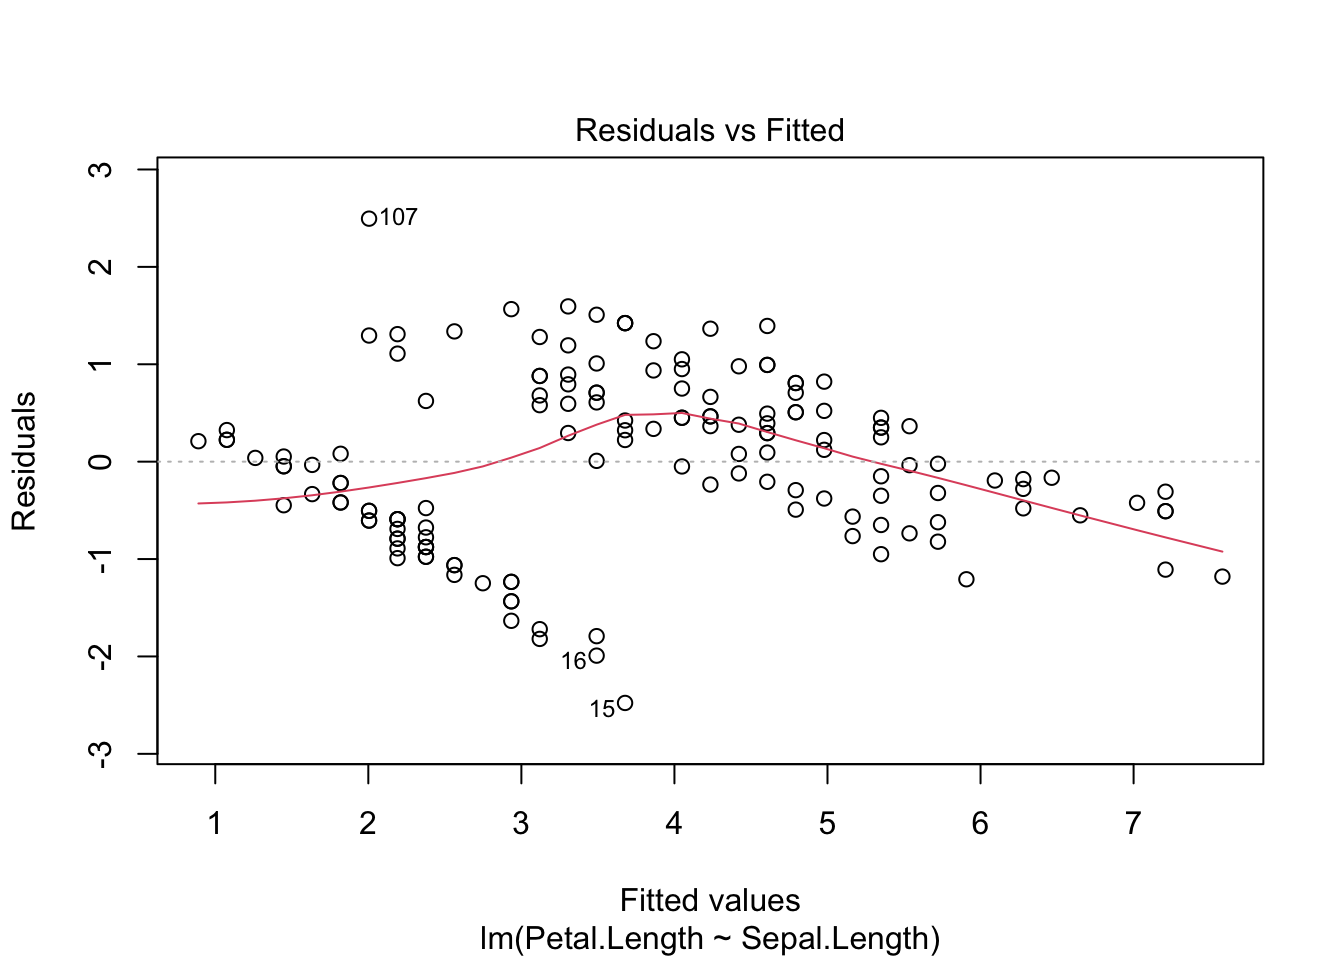
\includegraphics{DataExploration_files/figure-latex/unnamed-chunk-20-1.pdf} 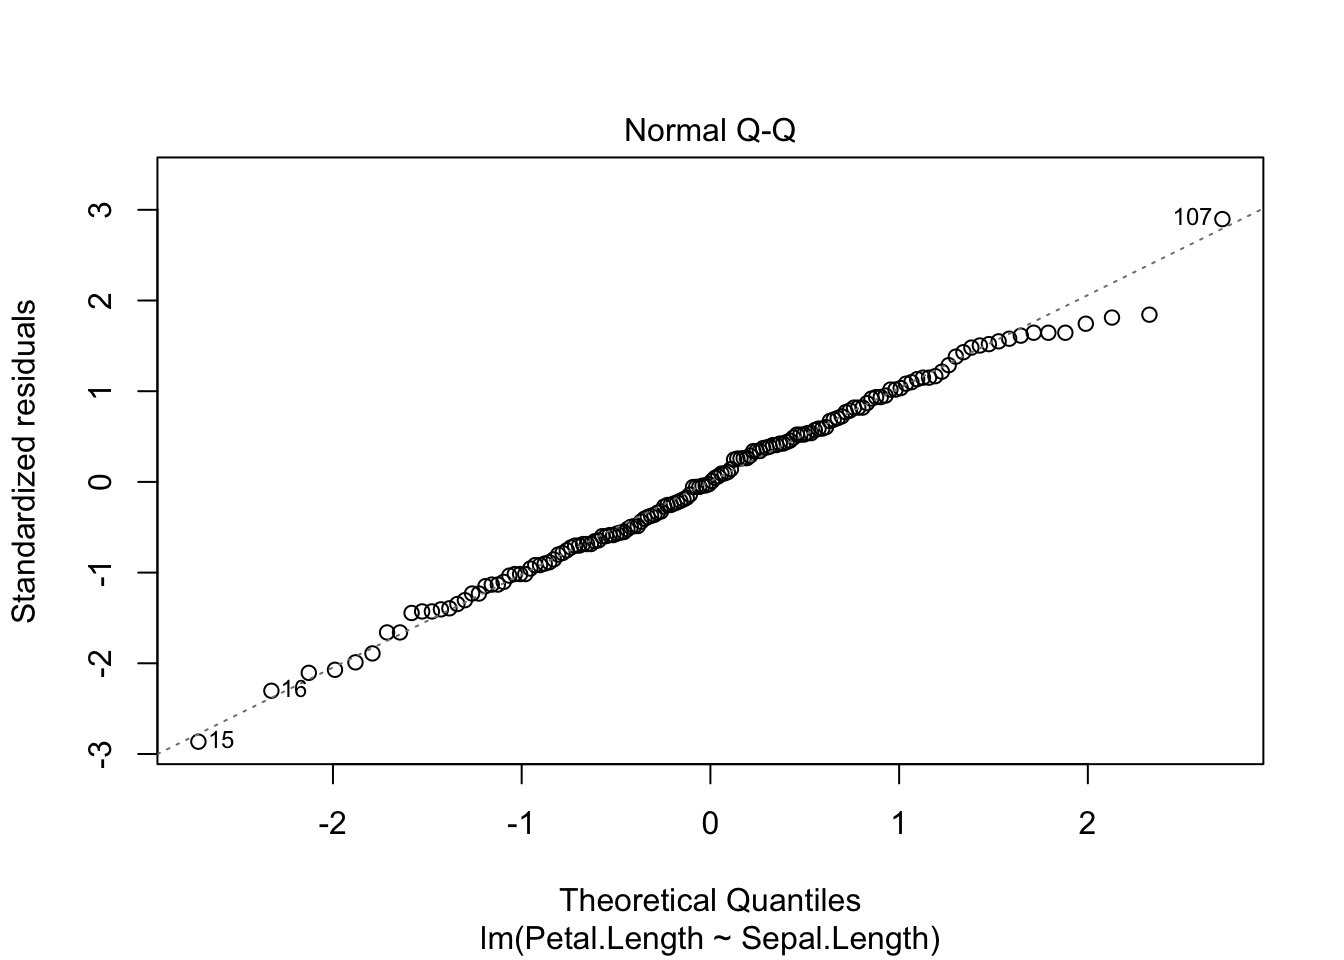
\includegraphics{DataExploration_files/figure-latex/unnamed-chunk-20-2.pdf} 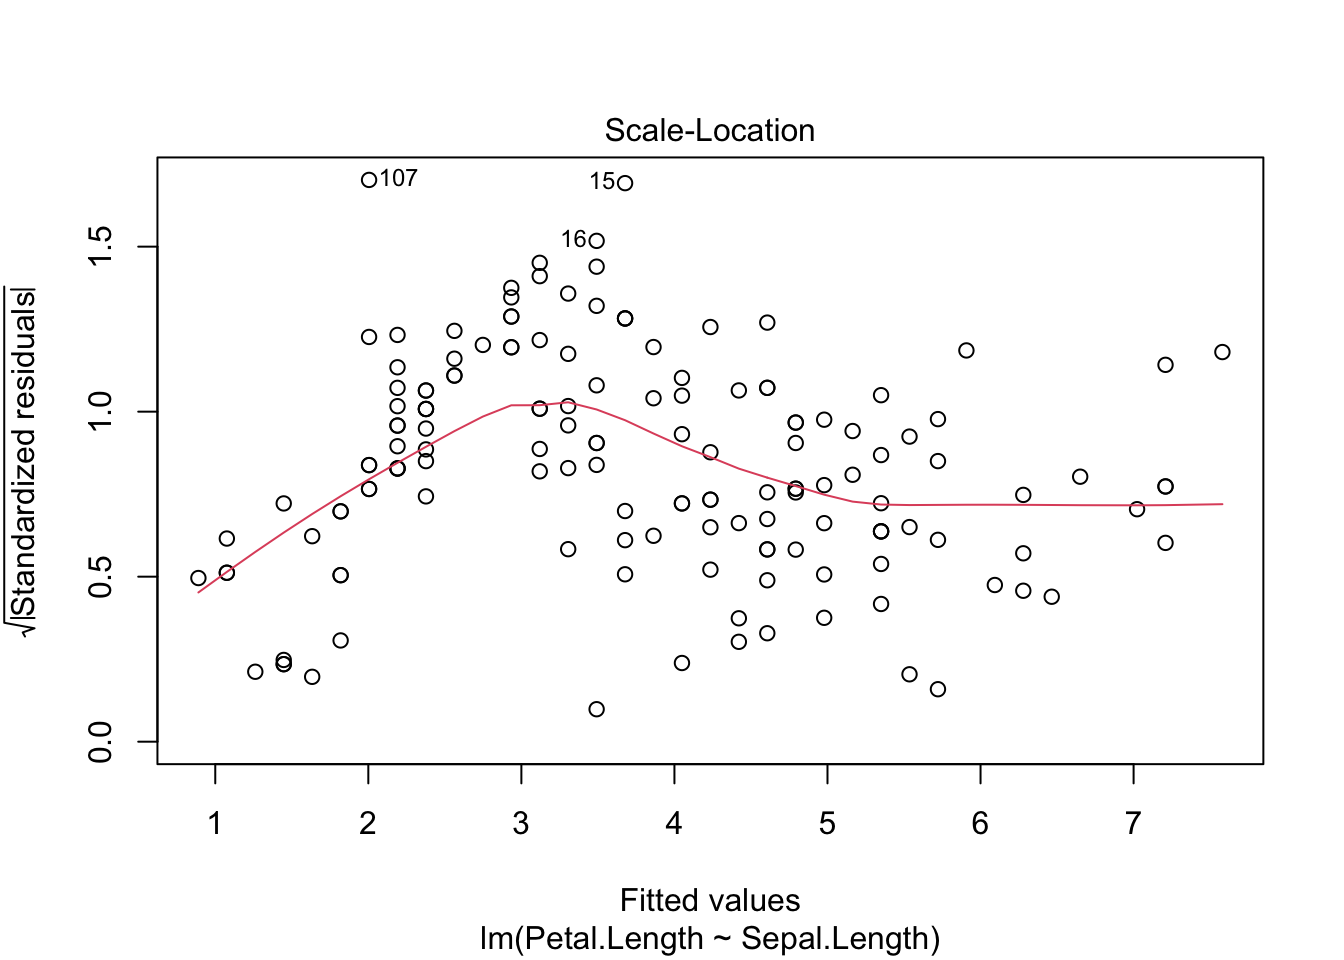
\includegraphics{DataExploration_files/figure-latex/unnamed-chunk-20-3.pdf} 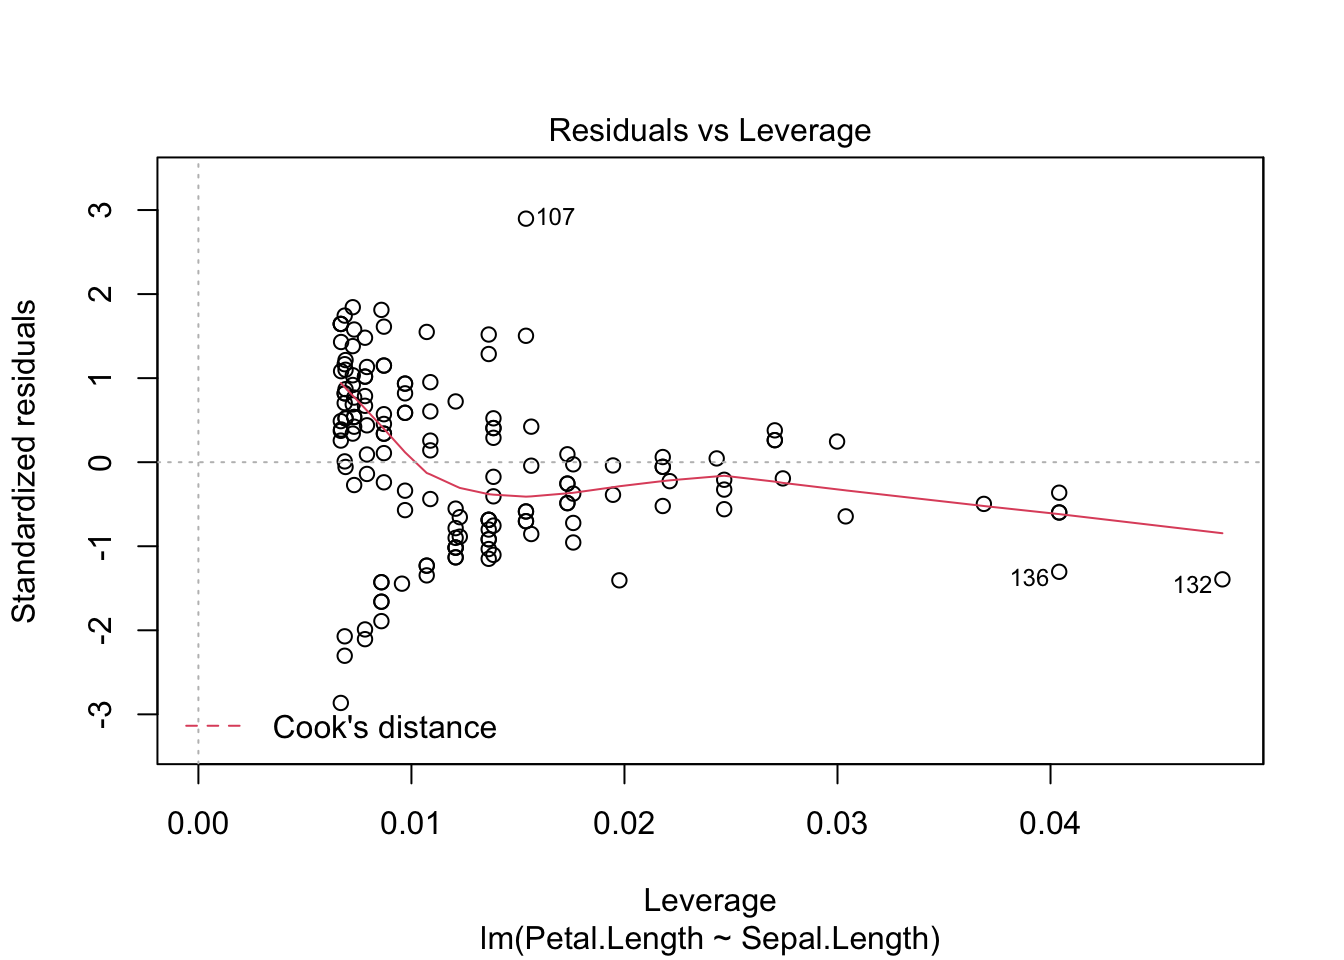
\includegraphics{DataExploration_files/figure-latex/unnamed-chunk-20-4.pdf}

Ok, that's it, I have almost all that I wanted ! We'll cover the rest at the end of the week !

\hypertarget{exercise}{%
\subsubsection{Exercise}\label{exercise}}

On the \texttt{iris} dataset, use the \texttt{kmeans} function to cluster the flowers with respect to Sepal.Length and Petal.Length and try to find your way in the resulting object.

\hypertarget{manip}{%
\chapter{Data manipulation}\label{manip}}

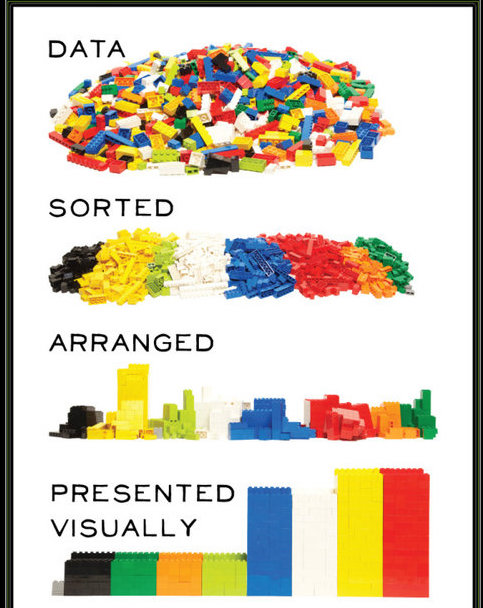
\includegraphics{img/data-viz.jpg}

In order to manipulate and wrangle data, there are (at least) 3 frameworks available :

\begin{itemize}
\tightlist
\item
  Base R (not covered) : similar to Pandas
\item
  Tidyverse/dplyr : high level interface
\item
  \texttt{data.table} : less friendly user interface but amazingly optimized
\end{itemize}

We'll cover the tidyverse approach as it provides a very nice and coherent framework for more than data manipulation. The ``tidy'' comes an original \href{http://www.jstatsoft.org/v59/i10/paper}{paper from Hadley Wickham} which sets those common sense principles

\begin{itemize}
\tightlist
\item
  Each variable must have its own column.
\item
  Each observation must have its own row.
\item
  Each value must have its own cell.
\end{itemize}

You can check further details and visualization on the \href{https://r4ds.had.co.nz/tidy-data.html}{R for data science online book}

Those principles have been largely adopted by the community (powered by Rstudio) and created a full parallel dialect in R for almost all data science tasks : the \href{https://www.tidyverse.org/}{\textbf{tidyverse}} which offers a coherent set of features that are, in addition, often nicely optimized (written in C++)

\hypertarget{import}{%
\section{Import}\label{import}}

\hypertarget{text-files}{%
\subsection{Text files}\label{text-files}}

You can either use the basic \texttt{read.table} and related functions (eg \texttt{read.csv}) which work pretty fine. If the file is large, you might consider tools from other package such as read\_csv and others from the \texttt{readr} package (part of the tidyverse)

\begin{Shaded}
\begin{Highlighting}[]
\NormalTok{dat <-}\StringTok{ }\KeywordTok{read.csv}\NormalTok{(}\StringTok{"Data/Sports/Activities.csv"}\NormalTok{,}\DataTypeTok{header =}\NormalTok{ T)}
\KeywordTok{head}\NormalTok{(dat)}
\end{Highlighting}
\end{Shaded}

\begin{verbatim}
##   activityId       uuidMsb       uuidLsb                name activityType
## 1 5570974040  3.695224e+18 -7.098507e+18          En piscine lap_swimming
## 2 5566524321 -5.212790e+18 -8.140623e+18     Vienna Cyclisme      cycling
## 3 5561266034  1.271356e+18 -5.522844e+18 Korneuburg Cyclisme      cycling
## 4 5555881653 -2.923938e+18 -4.676832e+18       Vienna Course      running
## 5 5551811953  7.859043e+18 -7.909532e+18      Zwift - London virtual_ride
## 6 5551052200 -9.554086e+17 -6.866435e+18          En piscine lap_swimming
##   userProfileId timeZoneId beginTimestamp eventTypeId   rule sportType
## 1       1141258        124   1.600700e+12           9 public   GENERIC
## 2       1141258        124   1.600602e+12           9 public   CYCLING
## 3       1141258        124   1.600523e+12           9 public   CYCLING
## 4       1141258        124   1.600439e+12           9 public   RUNNING
## 5       1141258        124   1.600362e+12           9 public   GENERIC
## 6       1141258        124   1.600353e+12           9 public   GENERIC
##   startTimeGmt startTimeLocal duration distance elevationGain elevationLoss
## 1 1.600700e+12   1.600708e+12  3640221   300000            NA            NA
## 2 1.600602e+12   1.600609e+12 15064570 12293220        200100        196800
## 3 1.600523e+12   1.600530e+12 10382433  8360927         74500         74200
## 4 1.600439e+12   1.600447e+12  5393830  1792890         42600         42500
## 5 1.600362e+12   1.600369e+12  3626825  3492347         16000             0
## 6 1.600353e+12   1.600360e+12  3359145   285000            NA            NA
##   avgSpeed maxSpeed avgHr maxHr  calories startLongitude startLatitude
## 1   0.0986   0.1122    NA    NA  2547.532             NA            NA
## 2   0.8160   1.9315   144   176 16345.268       16.31524      48.20915
## 3   0.8053   1.9557   117   161  8744.572       16.33986      48.34994
## 4   0.3324   1.2475   155   176  4923.274       16.31587      48.21432
## 5   0.9629   1.6364   138   163  3083.855        0.00000       0.00000
## 6   0.1011   0.3524    NA    NA  2505.632             NA            NA
##   aerobicTrainingEffect avgFractionalCadence maxFractionalCadence
## 1                    NA               0.0000                    0
## 2                   3.5               0.0000                    0
## 3                   2.4               0.0000                    0
## 4                   3.0               0.1875                    0
## 5                   0.0               0.0000                    0
## 6                    NA               0.0000                    0
##   elapsedDuration movingDuration anaerobicTrainingEffect   deviceId
## 1         3955901        3099653                      NA 3968818126
## 2        16176575       15000179                     0.0 3968818126
## 3        11319866       10356078                     0.0 3968818126
## 4         5538505        5389603                     0.2 3968818126
## 5         3629000        3611000                      NA 3825981698
## 6         3585826        2858951                      NA 3968818126
##   minTemperature maxTemperature minElevation maxElevation        locationName
## 1             25             26           NA           NA                <NA>
## 2             19             29        18480        95480              Vienna
## 3             18             29        13980        32200          Korneuburg
## 4             19             27        24920        54400              Vienna
## 5             NA             NA          300         3420 City of Westminster
## 6             26             27           NA           NA                <NA>
##   maxVerticalSpeed lapCount endLongitude endLatitude activeSets totalSets
## 1               NA       34           NA          NA         NA        NA
## 2       0.43999939       25     16.25314    48.20399         NA        NA
## 3       0.34000092       17     16.38793    48.38009         NA        NA
## 4       0.08000183       18     16.31980    48.22264         NA        NA
## 5       0.16000004        1           NA          NA         NA        NA
## 6               NA       32           NA          NA         NA        NA
##   totalReps purposeful autoCalcCalories favorite    pr elevationCorrected
## 1        NA      FALSE            FALSE    FALSE FALSE              FALSE
## 2        NA      FALSE            FALSE    FALSE FALSE              FALSE
## 3        NA      FALSE            FALSE    FALSE FALSE              FALSE
## 4        NA      FALSE            FALSE    FALSE FALSE              FALSE
## 5        NA      FALSE            FALSE    FALSE FALSE              FALSE
## 6        NA      FALSE            FALSE    FALSE FALSE              FALSE
##   atpActivity parent maxRunCadence steps avgVerticalOscillation
## 1       FALSE  FALSE            NA    NA                     NA
## 2       FALSE  FALSE            NA    NA                     NA
## 3       FALSE  FALSE            NA    NA                     NA
## 4       FALSE  FALSE           104 15620                     NA
## 5       FALSE  FALSE            NA    NA                     NA
## 6       FALSE  FALSE            NA    NA                     NA
##   avgGroundContactTime avgStrideLength vO2MaxValue avgVerticalRatio
## 1                   NA              NA          NA               NA
## 2                   NA              NA          72               NA
## 3                   NA              NA          71               NA
## 4                   NA        115.6389          58               NA
## 5                   NA              NA          NA               NA
## 6                   NA              NA          NA               NA
##   avgGroundContactBalance avgDoubleCadence maxDoubleCadence avgPower
## 1                      NA               NA               NA       NA
## 2                      NA               NA               NA      260
## 3                      NA               NA               NA      202
## 4                      NA          172.375              208       NA
## 5                      NA               NA               NA      212
## 6                      NA               NA               NA       NA
##   avgBikeCadence maxBikeCadence strokes normPower avgLeftBalance
## 1             NA             NA    1198        NA             NA
## 2             83            114   17968  296.0000          49.92
## 3             82            107   12571  231.0000          49.90
## 4             NA             NA      NA        NA             NA
## 5             91            114       0  218.3049             NA
## 6             NA             NA    1152        NA             NA
##   avgRightBalance max20MinPower trainingStressScore intensityFactor
## 1              NA            NA                  NA              NA
## 2           50.08      375.1583               291.4           0.835
## 3           50.10      242.7692               122.8           0.653
## 4              NA            NA                  NA              NA
## 5              NA      221.0525                  NA              NA
## 6              NA            NA                  NA              NA
##   lactateThresholdBpm lactateThresholdSpeed avgStrokes activeLengths avgSwolf
## 1                  NA                    NA       23.0            60       74
## 2                  NA                    NA         NA            NA       NA
## 3                  NA                    NA         NA            NA       NA
## 4                  NA                    NA         NA            NA       NA
## 5                  NA                    NA         NA            NA       NA
## 6                  NA                    NA       22.6            57       72
##   poolLength avgStrokeDistance avgSwimCadence maxSwimCadence maxFtp workoutId
## 1       5000               217             27             29     NA        NA
## 2         NA                NA             NA             NA     NA        NA
## 3         NA                NA             NA             NA     NA        NA
## 4         NA                NA             NA             NA     NA        NA
## 5         NA                NA             NA             NA     NA        NA
## 6       5000               221             27             30     NA        NA
##   decoDive parentId avgVerticalSpeed maxDepth avgDepth surfaceInterval
## 1       NA       NA               NA       NA       NA              NA
## 2       NA       NA               NA       NA       NA              NA
## 3       NA       NA               NA       NA       NA              NA
## 4       NA       NA               NA       NA       NA              NA
## 5       NA       NA               NA       NA       NA              NA
## 6       NA       NA               NA       NA       NA              NA
##   floorsDescended bottomTime
## 1              NA         NA
## 2              NA         NA
## 3              NA         NA
## 4              NA         NA
## 5              NA         NA
## 6              NA         NA
\end{verbatim}

You have many options to deal with issues :

\begin{itemize}
\tightlist
\item
  \texttt{sep} to specify the separator (\texttt{\textbackslash{}t} for tabulation, \texttt{\textquotesingle{};\textquotesingle{}} for semicolon\ldots{} )
\item
  \texttt{dec} the decimal separator
\item
  \texttt{encoding} the file encoding (special characters from windows/unix systems can be misdetected)
\item
  \texttt{colClasses} to force one column to be imported in another type than what is detected
\item
  \texttt{help(read.table)} for more options !
\end{itemize}

\hypertarget{excel-files}{%
\subsection{Excel files}\label{excel-files}}

You can import excel files (.xls and .xlsx) with the \texttt{readxl} package

\begin{Shaded}
\begin{Highlighting}[]
\NormalTok{readxl}\OperatorTok{::}\KeywordTok{read_excel}\NormalTok{(}\StringTok{"Data/Sports/Activities.xlsx"}\NormalTok{) }\OperatorTok\StringTok{ }
\StringTok{  }\KeywordTok{head}\NormalTok{()}
\end{Highlighting}
\end{Shaded}

\begin{verbatim}
## # A tibble: 6 x 89
##   activityId uuidMsb uuidLsb name  activityType userProfileId timeZoneId
##        <dbl> <chr>   <chr>   <chr> <chr>                <dbl>      <dbl>
## 1 5570974040 3.6952~ -7.098~ En p~ lap_swimming       1141258        124
## 2 5566524321 -5.212~ -8.140~ Vien~ cycling            1141258        124
## 3 5561266034 1.2713~ -5.522~ Korn~ cycling            1141258        124
## 4 5555881653 -2.923~ -4.676~ Vien~ running            1141258        124
## 5 5551811953 7.8590~ -7.909~ Zwif~ virtual_ride       1141258        124
## 6 5551052200 -9.554~ -6.866~ En p~ lap_swimming       1141258        124
## # ... with 82 more variables: beginTimestamp <chr>, eventTypeId <dbl>,
## #   rule <chr>, sportType <chr>, startTimeGmt <dbl>, startTimeLocal <chr>,
## #   duration <chr>, distance <chr>, elevationGain <chr>, elevationLoss <chr>,
## #   avgSpeed <chr>, maxSpeed <chr>, avgHr <chr>, maxHr <chr>, calories <chr>,
## #   startLongitude <chr>, startLatitude <chr>, aerobicTrainingEffect <chr>,
## #   avgFractionalCadence <chr>, maxFractionalCadence <chr>,
## #   elapsedDuration <chr>, movingDuration <chr>, anaerobicTrainingEffect <chr>,
## #   deviceId <dbl>, minTemperature <chr>, maxTemperature <chr>,
## #   minElevation <chr>, maxElevation <chr>, locationName <chr>,
## #   maxVerticalSpeed <chr>, lapCount <dbl>, endLongitude <chr>,
## #   endLatitude <chr>, activeSets <chr>, totalSets <chr>, totalReps <chr>,
## #   purposeful <chr>, autoCalcCalories <chr>, favorite <chr>, pr <chr>,
## #   elevationCorrected <chr>, atpActivity <chr>, parent <chr>,
## #   maxRunCadence <chr>, steps <chr>, avgVerticalOscillation <chr>,
## #   avgGroundContactTime <chr>, avgStrideLength <chr>, vO2MaxValue <chr>,
## #   avgVerticalRatio <chr>, avgGroundContactBalance <chr>,
## #   avgDoubleCadence <chr>, maxDoubleCadence <chr>, avgPower <chr>,
## #   avgBikeCadence <chr>, maxBikeCadence <chr>, strokes <chr>, normPower <chr>,
## #   avgLeftBalance <chr>, avgRightBalance <chr>, max20MinPower <chr>,
## #   trainingStressScore <chr>, intensityFactor <chr>,
## #   lactateThresholdBpm <chr>, lactateThresholdSpeed <chr>, avgStrokes <chr>,
## #   activeLengths <chr>, avgSwolf <chr>, poolLength <chr>,
## #   avgStrokeDistance <chr>, avgSwimCadence <chr>, maxSwimCadence <chr>,
## #   maxFtp <chr>, workoutId <chr>, decoDive <chr>, parentId <chr>,
## #   avgVerticalSpeed <chr>, maxDepth <chr>, avgDepth <chr>,
## #   surfaceInterval <chr>, floorsDescended <chr>, bottomTime <chr>
\end{verbatim}

Options :

\begin{itemize}
\tightlist
\item
  \texttt{sheet} to select whioch you want to import
\item
  \texttt{range} : the ``zone'' of the sheet you want to import (beginning and ending row/column to be provided)
\item
  \texttt{col\_types} to specify the types of the column if misdetected
\item
  \texttt{?readxl::read\_excel} for more information
\end{itemize}

\hypertarget{more-formats}{%
\subsection{More formats}\label{more-formats}}

The \texttt{readr} package provides other convenient functions to read the most common (open) formats. With \texttt{haven}, you can also read data from proprietary formats (SPSS, SAS, Stat,\ldots).

JSON files can be read with for example \texttt{rjsonlite} and we will use it in an applicaiton example.

XML and HTML files can be parsed with the \texttt{xml2}package.

\hypertarget{read-from-databases-big-data}{%
\subsection{Read from databases / big data}\label{read-from-databases-big-data}}

This is a huge topic that we will only mention here, but for (almost) each database engine, there is a package available in order to be able to read data from databases

\begin{itemize}
\tightlist
\item
  General purpose : \texttt{odbc}, \texttt{RODBC}, \texttt{DBI} \(\rightarrow\) you will need to install the DB's drivers
\item
  Dedicated : \texttt{RSQLite}, \texttt{RPostgres}, \texttt{RMariaDB} (can be used for mySQL too)\ldots{} \(\rightarrow\) drivers included
\end{itemize}

With the 3 first package, you can connect to ``monolith'' databases, as well as to distributed databases. You can find more information on the \href{https://db.rstudio.com/}{Rstudio website}. Another interesting resources is the \href{https://cran.r-project.org/web/packages/dbplyr/vignettes/dbplyr.html}{\texttt{dbplyr} vignette}, that describes how to connect to a database and query it using \texttt{dplyr}'s verbs.

In addition, the \texttt{sparlyr} package allows you to interact with a spark cluster (using \texttt{dplyr\ syntax})

\hypertarget{the-grammar-of-data-manipulation}{%
\section{The grammar of data manipulation}\label{the-grammar-of-data-manipulation}}

\textbf{Alert :} After this section, pandas will appear much less appealing\ldots.
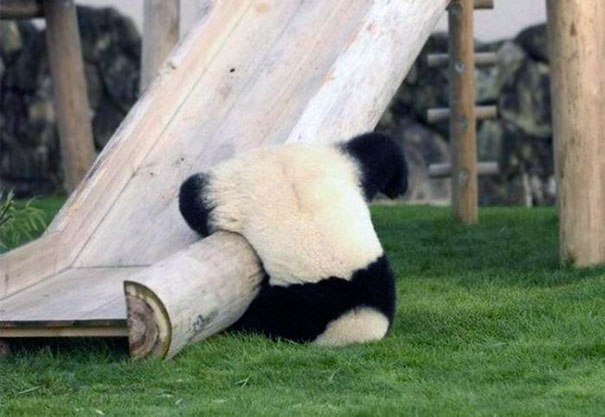
\includegraphics{img/pandas-fun.jpg}

Following the tidy data principles, \texttt{dplyr} implements an actual grammar of data manipulation with verbs and human-readable syntax.

\hypertarget{the-pipe}{%
\subsection{The pipe}\label{the-pipe}}


\includegraphics{img/pipe.png}

The first operator to know is the \emph{pipe} operator, \texttt{\%\textgreater{}\%} which allows you to redirect the output of a command ``to the right'' and hence create readable chains of commands.
Let's extract the last 3 characters of ``hello world''

First solution : create useless objects

\begin{Shaded}
\begin{Highlighting}[]
\NormalTok{char <-}\StringTok{ "hello world"}
\NormalTok{rev_char <-}\StringTok{ }\NormalTok{stringi}\OperatorTok{::}\KeywordTok{stri_reverse}\NormalTok{(char)}
\NormalTok{sub3 <-}\StringTok{ }\KeywordTok{substr}\NormalTok{(rev_char,}\DecValTok{1}\NormalTok{,}\DecValTok{3}\NormalTok{)}
\NormalTok{stringi}\OperatorTok{::}\KeywordTok{stri_reverse}\NormalTok{(sub3)}
\end{Highlighting}
\end{Shaded}

\begin{verbatim}
## [1] "rld"
\end{verbatim}

Second solution : where's the beginning ????

\begin{Shaded}
\begin{Highlighting}[]
\NormalTok{stringi}\OperatorTok{::}\KeywordTok{stri_reverse}\NormalTok{(}\KeywordTok{substr}\NormalTok{(stringi}\OperatorTok{::}\KeywordTok{stri_reverse}\NormalTok{(}\StringTok{"Hello World"}\NormalTok{),}\DecValTok{1}\NormalTok{,}\DecValTok{3}\NormalTok{))}
\end{Highlighting}
\end{Shaded}

\begin{verbatim}
## [1] "rld"
\end{verbatim}

Third solution : using the pipe

\begin{Shaded}
\begin{Highlighting}[]
\StringTok{"Hello world"} \OperatorTok\StringTok{ }
\StringTok{  }\NormalTok{stringi}\OperatorTok{::}\KeywordTok{stri_reverse}\NormalTok{() }\OperatorTok\StringTok{ }
\StringTok{  }\KeywordTok{substr}\NormalTok{(}\DecValTok{1}\NormalTok{,}\DecValTok{3}\NormalTok{) }\OperatorTok\StringTok{ }
\StringTok{  }\NormalTok{stringi}\OperatorTok{::}\KeywordTok{stri_reverse}\NormalTok{()}
\end{Highlighting}
\end{Shaded}

\begin{verbatim}
## [1] "rld"
\end{verbatim}

Under the hood : the dot represents the result of the previous step and can be placed somewhere else in the next function (rather than the first argument)

\begin{Shaded}
\begin{Highlighting}[]
\StringTok{"Hello world"} \OperatorTok\StringTok{ }
\StringTok{  }\NormalTok{stringi}\OperatorTok{::}\KeywordTok{stri_reverse}\NormalTok{(.) }\OperatorTok\StringTok{ }
\StringTok{  }\KeywordTok{substr}\NormalTok{(.,}\DecValTok{1}\NormalTok{,}\DecValTok{3}\NormalTok{) }\OperatorTok\StringTok{ }
\StringTok{  }\NormalTok{stringi}\OperatorTok{::}\KeywordTok{stri_reverse}\NormalTok{(.)}
\end{Highlighting}
\end{Shaded}

\begin{verbatim}
## [1] "rld"
\end{verbatim}

\hypertarget{the-verbs-of-manipulation}{%
\subsection{The verbs of manipulation}\label{the-verbs-of-manipulation}}

What do you do with data ?

\begin{itemize}
\tightlist
\item
  Select columns \(\rightarrow\) \texttt{select()}
\item
  Filter rows \(\rightarrow\) \texttt{filter()}
\item
  Create / modify columns \(\rightarrow\) \texttt{mutate()}
\item
  Compute summaries of the columns \(\rightarrow\) \texttt{summarise()}
\item
  Do group-wise operations \(\rightarrow\) \texttt{group\_by()}
\item
  Join with other tables \(\rightarrow\) \texttt{left\_join()},\texttt{right\_join()}, \texttt{inner\_join()}, \texttt{anti\_join()}, \texttt{full\_join()}
\end{itemize}

I have the verbs, now I can associate them to make a sentence ! All those functions take as first argument a dataframe, which makes it very easy when chaining them with the pipe.

\begin{Shaded}
\begin{Highlighting}[]
\KeywordTok{read.csv}\NormalTok{(}\StringTok{"Data/Sports/Activities.csv"}\NormalTok{) }\OperatorTok\StringTok{ }
\StringTok{  }\KeywordTok{select}\NormalTok{(activityType,avgSpeed,distance,startLongitude,startLatitude,sportType) }\OperatorTok\StringTok{ }\CommentTok{#select some metrics}
\StringTok{  }\KeywordTok{mutate}\NormalTok{(}\DataTypeTok{distance=}\NormalTok{distance}\OperatorTok{/}\DecValTok{100}\NormalTok{) }\OperatorTok\StringTok{ }\CommentTok{# distances are in decameter (?)}
\StringTok{  }\KeywordTok{filter}\NormalTok{(activityType}\OperatorTok{!=}\StringTok{"other"}\NormalTok{) }\OperatorTok\StringTok{ }\CommentTok{# remove activities "other}
\StringTok{  }\KeywordTok{group_by}\NormalTok{(activityType) }\OperatorTok\StringTok{ }
\StringTok{  }\KeywordTok{summarise}\NormalTok{(}\DataTypeTok{total_dist=}\KeywordTok{mean}\NormalTok{(distance))}
\end{Highlighting}
\end{Shaded}

\begin{verbatim}
## # A tibble: 22 x 2
##    activityType            total_dist
##    <chr>                        <dbl>
##  1 cross_country_skiing_ws     16717.
##  2 cycling                     34124.
##  3 cyclocross                  41210.
##  4 hiking                      10678.
##  5 indoor_cardio                  NA 
##  6 indoor_cycling                 NA 
##  7 indoor_running               2311.
##  8 lap_swimming                 3014.
##  9 multi_sport                 63873.
## 10 open_water_swimming          2359.
## # ... with 12 more rows
\end{verbatim}

\hypertarget{filter-conditions}{%
\subsection{Filter : conditions}\label{filter-conditions}}

This is the way you write conditions in R :

\begin{longtable}[]{@{}ll@{}}
\toprule
Syntax & Condition\tabularnewline
\midrule
\endhead
== & Equality test\tabularnewline
!= & Different than\tabularnewline
\%in\% c(\ldots) & Is in this list of values\tabularnewline
\(>, >=\) \(<, <=\) & Greater/less than\tabularnewline
! (x \%in\% c(\ldots)) & Not in the list\tabularnewline
\bottomrule
\end{longtable}

\hypertarget{mutate}{%
\subsection{Mutate}\label{mutate}}

Most of the data manipulation will be done in a mutate statement. This is where you can create additional columns, modify the ones existing. You can do any kind of transformation you want with this one. Depending on the type of the data, here are some additional packages that will help you :

\begin{itemize}
\tightlist
\item
  \texttt{lubridate} to easily handle date variables
\item
  \texttt{forcats} to handle factors (categorical variables)
\item
  \texttt{stringr} (and \texttt{stringi}) to handle strings variables and work with regular expressions
\item
  \texttt{ifelse()} and \texttt{case\_when()} to handle conditional operations
\end{itemize}

\begin{Shaded}
\begin{Highlighting}[]
\KeywordTok{require}\NormalTok{(lubridate)}
\KeywordTok{require}\NormalTok{(stringr)}

\NormalTok{dat <-}\StringTok{ }\NormalTok{dat }\OperatorTok\StringTok{ }
\StringTok{  }\KeywordTok{mutate}\NormalTok{(}\DataTypeTok{start_time=}\KeywordTok{as_datetime}\NormalTok{(startTimeLocal}\OperatorTok{/}\DecValTok{1000}\NormalTok{), }\CommentTok{# create a timestamp}
         \DataTypeTok{date =} \KeywordTok{floor_date}\NormalTok{(start_time,}\StringTok{"day"}\NormalTok{), }\CommentTok{# round to the day}
         \DataTypeTok{is_bike=}\KeywordTok{ifelse}\NormalTok{(activityType }\OperatorTok
\StringTok{                          }\KeywordTok{c}\NormalTok{(}\StringTok{"cycling"}\NormalTok{,}\StringTok{"virtual_ride"}\NormalTok{,}\StringTok{"indoor_cycling"}\NormalTok{,}\StringTok{"road_biking"}\NormalTok{,}\StringTok{"cyclocross"}\NormalTok{),T,F),}
         \CommentTok{# is it bike or not ?}
         \DataTypeTok{is_run =} \KeywordTok{str_detect}\NormalTok{(activityType,}\StringTok{"running|hicking"}\NormalTok{),}
         \DataTypeTok{activity_recoded =} \KeywordTok{case_when}\NormalTok{(is_bike }\OperatorTok{~}\StringTok{ "Bike"}\NormalTok{,}
\NormalTok{                                      is_run }\OperatorTok{~}\StringTok{ "Run"}\NormalTok{,}
                                      \KeywordTok{str_detect}\NormalTok{(activityType,}\StringTok{"swim"}\NormalTok{) }\OperatorTok{~}\StringTok{"Swim"}\NormalTok{,}
                                      \OtherTok{TRUE} \OperatorTok{~}\StringTok{ "Other"}\NormalTok{))}
\end{Highlighting}
\end{Shaded}

\hypertarget{summarize}{%
\subsection{Summarize}\label{summarize}}

This operation consists in summarizing several rows ofinto one or more synthetic value(s). We will cover the topic more in detail \ref{stats} but the most common summary function that you can use are :

\begin{itemize}
\tightlist
\item
  For continuous variables : average, sum, median, standard deviation, interquartile range (IQR), concentration indexes,\ldots{}
\item
  For categorical variables : count, count distinct, concentration indexes,\ldots{}
\end{itemize}

Simple summary statistics over one numerical variable :

\begin{Shaded}
\begin{Highlighting}[]
\NormalTok{dat }\OperatorTok\StringTok{ }\KeywordTok{summarise}\NormalTok{(}\DataTypeTok{total_distance=}\KeywordTok{sum}\NormalTok{(distance)) }\CommentTok{# Oups}
\end{Highlighting}
\end{Shaded}

\begin{verbatim}
##   total_distance
## 1             NA
\end{verbatim}

\begin{Shaded}
\begin{Highlighting}[]
\NormalTok{dat }\OperatorTok\StringTok{ }\KeywordTok{summarise}\NormalTok{(}\DataTypeTok{total_distance=}\KeywordTok{sum}\NormalTok{(distance,}\DataTypeTok{na.rm =}\NormalTok{ T))}
\end{Highlighting}
\end{Shaded}

\begin{verbatim}
##   total_distance
## 1    10693637146
\end{verbatim}

\begin{Shaded}
\begin{Highlighting}[]
\NormalTok{dat }\OperatorTok\StringTok{ }\KeywordTok{summarise}\NormalTok{(}\DataTypeTok{avg_distance=}\KeywordTok{mean}\NormalTok{(distance,}\DataTypeTok{na.rm =}\NormalTok{ T))}
\end{Highlighting}
\end{Shaded}

\begin{verbatim}
##   avg_distance
## 1      1941826
\end{verbatim}

\begin{Shaded}
\begin{Highlighting}[]
\NormalTok{dat }\OperatorTok\StringTok{ }\KeywordTok{summarise}\NormalTok{(}\DataTypeTok{median_distance=}\KeywordTok{median}\NormalTok{(distance,}\DataTypeTok{na.rm =}\NormalTok{ T))}
\end{Highlighting}
\end{Shaded}

\begin{verbatim}
##   median_distance
## 1         1186419
\end{verbatim}

\hypertarget{manipulate-several-data-in-the-same-time}{%
\subsection{Manipulate several data in the same time}\label{manipulate-several-data-in-the-same-time}}

With all previous verbs above, you can use the \texttt{across} function to apply the same operation over a bunch of columns that you can select depending a simple enumeration or a condition (on their type or their name). This is a really powerful tool !

Example : we will convert all columns that are identifiers as character variables because the numbers have no meaning

\begin{Shaded}
\begin{Highlighting}[]
\NormalTok{dat <-}\StringTok{ }\NormalTok{dat }\OperatorTok\StringTok{ }
\StringTok{  }\KeywordTok{mutate}\NormalTok{(}\KeywordTok{across}\NormalTok{(}\KeywordTok{c}\NormalTok{(}\KeywordTok{contains}\NormalTok{(}\StringTok{"Id"}\NormalTok{),}\KeywordTok{contains}\NormalTok{(}\StringTok{"uuid"}\NormalTok{)),}
\NormalTok{                as.character))}
\CommentTok{# Other stupid examples}
\NormalTok{dat }\OperatorTok\StringTok{  }\KeywordTok{summarise}\NormalTok{(}\KeywordTok{across}\NormalTok{(}\KeywordTok{where}\NormalTok{(is.numeric),}
                          \ControlFlowTok{function}\NormalTok{(xx) }\KeywordTok{sum}\NormalTok{(xx,}\DataTypeTok{na.rm=}\NormalTok{T)))}
\end{Highlighting}
\end{Shaded}

\begin{verbatim}
##   beginTimestamp startTimeGmt startTimeLocal    duration    distance
## 1   8.021486e+15 8.036783e+15   8.036814e+15 22850917079 10693637146
##   elevationGain elevationLoss avgSpeed maxSpeed  avgHr  maxHr calories
## 1     163374842     149923907 2186.754 113881.5 538175 637627 20569669
##   startLongitude startLatitude aerobicTrainingEffect avgFractionalCadence
## 1        18707.3      190193.1                7579.3             383.8125
##   maxFractionalCadence elapsedDuration movingDuration anaerobicTrainingEffect
## 1                170.5     11995810258     6623490405                   276.1
##   minTemperature maxTemperature minElevation maxElevation maxVerticalSpeed
## 1          46890          65603     35504232     66534189         322.7602
##   lapCount endLongitude endLatitude activeSets totalSets totalReps
## 1    26369     10138.19    39058.89          0         0         0
##   maxRunCadence    steps avgVerticalOscillation avgGroundContactTime
## 1         81893 27827620                5202.02             149787.7
##   vO2MaxValue avgVerticalRatio avgGroundContactBalance avgDoubleCadence
## 1       50052          4590.83                29360.86         124685.3
##   maxDoubleCadence avgPower avgBikeCadence maxBikeCadence  strokes normPower
## 1           163305   159062         120499         160192 11984172  172253.5
##   avgLeftBalance avgRightBalance max20MinPower trainingStressScore
## 1       29746.24        29853.76      178191.6            146746.6
##   intensityFactor lactateThresholdBpm lactateThresholdSpeed avgStrokes
## 1         640.338               12296               28.8716   36334.99
##   activeLengths avgSwolf poolLength avgStrokeDistance avgSwimCadence
## 1         82178    38881    2028199            113919          21590
##   maxSwimCadence maxFtp avgVerticalSpeed maxDepth avgDepth surfaceInterval
## 1          28979  28273                0        0        0               0
##   floorsDescended bottomTime
## 1               0          0
\end{verbatim}

\hypertarget{lets-import-and-wrangle-some-data}{%
\section{Let's import and wrangle some data !}\label{lets-import-and-wrangle-some-data}}

\hypertarget{the-data}{%
\subsection{The data}\label{the-data}}

We will work on the summary data of all past activities, which come in JSON files. So basically, the data is contained in (nested) lists. This is real word data, it's super messy and dirty !
You will have to :

\begin{itemize}
\tightlist
\item
  Import the data

  \begin{itemize}
  \tightlist
  \item
    Import one of the files using \texttt{jsonlite}
  \item
    Inspect and understand the structure of the list
  \item
    Get all the metrics that are included
  \item
    Figure out how to extract one specific metric for one activity
  \item
    Design a function to extract one metric for all activities contained in the JSON
  \item
    Design a function that will extract all metrics for all activities in the JSON
  \end{itemize}
\item
  Have a first cleaning of the data :

  \begin{itemize}
  \tightlist
  \item
    Check the distance/elevation variables ; what do you think ?
  \item
    Check the speed related variables : what do you think ?
  \item
    Check the calories variable and adjust it
  \item
    Check the duration related variable and adjust them to have minutes
  \item
    To help you figuring out, you can check an activity on garmin's site using \href{https://connect.garmin.com/modern/activity/5570974040}{this url} and change the activity number for the one you are inspecting
  \end{itemize}
\end{itemize}

A lot of reverse engineering ahead

\hypertarget{one-tool-you-will-need-lapply}{%
\subsection{\texorpdfstring{One tool you will need : \texttt{lapply()}}{One tool you will need : lapply()}}\label{one-tool-you-will-need-lapply}}

JSON are lists, and to iterate over list elements, you can either use \texttt{for} loops, which is highly \emph{not recommended} (R is no good with loops), or use \texttt{lapply()}. This function applies an operation over all elements of a list (or vector) and returns a list containing the result. You can also use \texttt{sapply()} which tries to coerce the result to a vector (if possible) if the expected output is not a list.

\begin{Shaded}
\begin{Highlighting}[]
\NormalTok{random_list <-}\StringTok{ }\KeywordTok{lapply}\NormalTok{(}\DecValTok{1}\OperatorTok{:}\DecValTok{100}\NormalTok{,}\ControlFlowTok{function}\NormalTok{(xx) }\KeywordTok{rnorm}\NormalTok{(}\DecValTok{100}\NormalTok{,xx,xx}\OperatorTok{/}\DecValTok{5}\NormalTok{))}
\KeywordTok{str}\NormalTok{(random_list[}\DecValTok{1}\OperatorTok{:}\DecValTok{5}\NormalTok{])}
\end{Highlighting}
\end{Shaded}

\begin{verbatim}
## List of 5
##  $ : num [1:100] 0.653 0.839 0.952 0.781 0.758 ...
##  $ : num [1:100] 1.305 2.453 0.972 2.419 1.907 ...
##  $ : num [1:100] 2.38 3.31 2.65 3.27 3.2 ...
##  $ : num [1:100] 4.95 3.46 4.23 5.08 5.37 ...
##  $ : num [1:100] 4.53 6.16 5.43 5.09 3.46 ...
\end{verbatim}

\textbf{Attention :} be careful with the squared brackets

\begin{Shaded}
\begin{Highlighting}[]
\NormalTok{random_list[}\DecValTok{1}\NormalTok{] }\CommentTok{# is a list}
\end{Highlighting}
\end{Shaded}

\begin{verbatim}
## [[1]]
##   [1] 0.6534956 0.8394734 0.9520231 0.7810726 0.7577881 1.1833391 1.2953283
##   [8] 1.1170205 0.7598093 0.9069834 1.0612687 0.4860967 0.9583442 1.2883162
##  [15] 0.7559182 0.9321351 1.1605419 0.8560776 1.2296965 1.1961155 1.1452899
##  [22] 0.8937648 1.1180562 1.1291864 1.1588141 0.7867302 1.2711314 0.8855429
##  [29] 1.2287864 0.7456788 0.9652640 0.7649677 0.9147540 0.8360354 1.3852953
##  [36] 1.0987498 0.9648034 0.6702452 0.8118263 0.8490696 1.1890466 1.0536951
##  [43] 0.9466750 1.1516804 1.2437038 1.3202114 1.0162013 0.3732095 0.8947668
##  [50] 1.1670457 1.0740586 0.9312860 1.1014046 1.2574607 0.8831380 1.2873086
##  [57] 1.3694036 1.2518263 1.1654449 0.5834937 0.6536882 0.9924216 1.1499586
##  [64] 1.1995749 1.4525548 0.9177919 1.0160229 0.7752616 1.0055312 0.9059316
##  [71] 0.8091390 0.6507289 0.9291632 0.9774625 0.9732182 0.9829048 1.1303813
##  [78] 1.0197155 0.8936495 0.7905860 1.1401793 1.1591278 1.2085776 1.3789252
##  [85] 1.1331738 0.7921537 1.3730403 0.8314237 0.9845227 0.7082945 0.9509746
##  [92] 1.1636481 1.0714989 0.9785293 1.0279219 1.0541376 1.1354783 0.8092468
##  [99] 0.8652608 0.7311741
\end{verbatim}

\begin{Shaded}
\begin{Highlighting}[]
\NormalTok{random_list[[}\DecValTok{1}\NormalTok{]] }\CommentTok{# is a vector}
\end{Highlighting}
\end{Shaded}

\begin{verbatim}
##   [1] 0.6534956 0.8394734 0.9520231 0.7810726 0.7577881 1.1833391 1.2953283
##   [8] 1.1170205 0.7598093 0.9069834 1.0612687 0.4860967 0.9583442 1.2883162
##  [15] 0.7559182 0.9321351 1.1605419 0.8560776 1.2296965 1.1961155 1.1452899
##  [22] 0.8937648 1.1180562 1.1291864 1.1588141 0.7867302 1.2711314 0.8855429
##  [29] 1.2287864 0.7456788 0.9652640 0.7649677 0.9147540 0.8360354 1.3852953
##  [36] 1.0987498 0.9648034 0.6702452 0.8118263 0.8490696 1.1890466 1.0536951
##  [43] 0.9466750 1.1516804 1.2437038 1.3202114 1.0162013 0.3732095 0.8947668
##  [50] 1.1670457 1.0740586 0.9312860 1.1014046 1.2574607 0.8831380 1.2873086
##  [57] 1.3694036 1.2518263 1.1654449 0.5834937 0.6536882 0.9924216 1.1499586
##  [64] 1.1995749 1.4525548 0.9177919 1.0160229 0.7752616 1.0055312 0.9059316
##  [71] 0.8091390 0.6507289 0.9291632 0.9774625 0.9732182 0.9829048 1.1303813
##  [78] 1.0197155 0.8936495 0.7905860 1.1401793 1.1591278 1.2085776 1.3789252
##  [85] 1.1331738 0.7921537 1.3730403 0.8314237 0.9845227 0.7082945 0.9509746
##  [92] 1.1636481 1.0714989 0.9785293 1.0279219 1.0541376 1.1354783 0.8092468
##  [99] 0.8652608 0.7311741
\end{verbatim}

\hypertarget{tidy-your-data}{%
\section{Tidy your data}\label{tidy-your-data}}

The data will almost never come in a ready-to-use format. Wrangling the data, beyond \emph{cleaning} it also sometimes imply to \emph{reshape} it so that it conforms to the tidy principles. For that you have 2 functions :

\begin{itemize}
\tightlist
\item
  \texttt{pivot\_longer()} which will convert columns into rows
\item
  \texttt{pivot\_wider()}, the reciprocate operation, which will convert rows into columns
\end{itemize}

For example, we can chose that an observation is the combination of an activity and a metric. This representation can be useful in some cases (see @ref(adv\_viz)).

\begin{Shaded}
\begin{Highlighting}[]
\NormalTok{dat_long <-}\StringTok{ }\NormalTok{dat }\OperatorTok\StringTok{ }
\StringTok{  }\KeywordTok{select}\NormalTok{(activityId,}\KeywordTok{where}\NormalTok{(is.numeric)) }\OperatorTok\StringTok{ }
\StringTok{  }\KeywordTok{pivot_longer}\NormalTok{(}\OperatorTok{-}\NormalTok{activityId,}\DataTypeTok{names_to=}\StringTok{"metric"}\NormalTok{,}\DataTypeTok{values_to=}\StringTok{"value"}\NormalTok{)}
\NormalTok{dat_long}
\end{Highlighting}
\end{Shaded}

\begin{verbatim}
## # A tibble: 363,924 x 3
##    activityId metric             value
##    <chr>      <chr>              <dbl>
##  1 5570974040 beginTimestamp  1.60e+12
##  2 5570974040 startTimeGmt    1.60e+12
##  3 5570974040 startTimeLocal  1.60e+12
##  4 5570974040 duration        3.64e+ 6
##  5 5570974040 distance        3.00e+ 5
##  6 5570974040 elevationGain  NA       
##  7 5570974040 elevationLoss  NA       
##  8 5570974040 avgSpeed        9.86e- 2
##  9 5570974040 maxSpeed        1.12e- 1
## 10 5570974040 avgHr          NA       
## # ... with 363,914 more rows
\end{verbatim}

With this format you can get summary statistics for all metrics also easily :

\begin{Shaded}
\begin{Highlighting}[]
\KeywordTok{group_by}\NormalTok{(dat_long,metric) }\OperatorTok\StringTok{ }
\StringTok{  }\KeywordTok{summarise}\NormalTok{(}\DataTypeTok{mean_val=}\KeywordTok{mean}\NormalTok{(value,}\DataTypeTok{na.rm=}\NormalTok{T))}
\end{Highlighting}
\end{Shaded}

\begin{verbatim}
## # A tibble: 66 x 2
##    metric                  mean_val
##    <chr>                      <dbl>
##  1 activeLengths            61.8   
##  2 activeSets                0     
##  3 aerobicTrainingEffect     2.88  
##  4 anaerobicTrainingEffect   0.298 
##  5 avgBikeCadence           91.2   
##  6 avgDepth                  0     
##  7 avgDoubleCadence        162.    
##  8 avgFractionalCadence      0.0696
##  9 avgGroundContactBalance  49.4   
## 10 avgGroundContactTime    252.    
## # ... with 56 more rows
\end{verbatim}

And you you can go back to the original format if you want :

\begin{Shaded}
\begin{Highlighting}[]
\KeywordTok{group_by}\NormalTok{(dat_long,metric) }\OperatorTok\StringTok{ }
\StringTok{  }\KeywordTok{summarise}\NormalTok{(}\DataTypeTok{mean_val=}\KeywordTok{mean}\NormalTok{(value,}\DataTypeTok{na.rm=}\NormalTok{T)) }\OperatorTok\StringTok{ }
\StringTok{  }\KeywordTok{pivot_wider}\NormalTok{(}\DataTypeTok{names_from =}\NormalTok{ metric,}\DataTypeTok{values_from=}\NormalTok{mean_val)}
\end{Highlighting}
\end{Shaded}

\begin{verbatim}
## # A tibble: 1 x 66
##   activeLengths activeSets aerobicTraining~ anaerobicTraini~ avgBikeCadence
##           <dbl>      <dbl>            <dbl>            <dbl>          <dbl>
## 1          61.8          0             2.88            0.298           91.2
## # ... with 61 more variables: avgDepth <dbl>, avgDoubleCadence <dbl>,
## #   avgFractionalCadence <dbl>, avgGroundContactBalance <dbl>,
## #   avgGroundContactTime <dbl>, avgHr <dbl>, avgLeftBalance <dbl>,
## #   avgPower <dbl>, avgRightBalance <dbl>, avgSpeed <dbl>,
## #   avgStrokeDistance <dbl>, avgStrokes <dbl>, avgSwimCadence <dbl>,
## #   avgSwolf <dbl>, avgVerticalOscillation <dbl>, avgVerticalRatio <dbl>,
## #   avgVerticalSpeed <dbl>, beginTimestamp <dbl>, bottomTime <dbl>,
## #   calories <dbl>, distance <dbl>, duration <dbl>, elapsedDuration <dbl>,
## #   elevationGain <dbl>, elevationLoss <dbl>, endLatitude <dbl>,
## #   endLongitude <dbl>, floorsDescended <dbl>, intensityFactor <dbl>,
## #   lactateThresholdBpm <dbl>, lactateThresholdSpeed <dbl>, lapCount <dbl>,
## #   max20MinPower <dbl>, maxBikeCadence <dbl>, maxDepth <dbl>,
## #   maxDoubleCadence <dbl>, maxElevation <dbl>, maxFractionalCadence <dbl>,
## #   maxFtp <dbl>, maxHr <dbl>, maxRunCadence <dbl>, maxSpeed <dbl>,
## #   maxSwimCadence <dbl>, maxTemperature <dbl>, maxVerticalSpeed <dbl>,
## #   minElevation <dbl>, minTemperature <dbl>, movingDuration <dbl>,
## #   normPower <dbl>, poolLength <dbl>, startLatitude <dbl>,
## #   startLongitude <dbl>, startTimeGmt <dbl>, startTimeLocal <dbl>,
## #   steps <dbl>, strokes <dbl>, surfaceInterval <dbl>, totalReps <dbl>,
## #   totalSets <dbl>, trainingStressScore <dbl>, vO2MaxValue <dbl>
\end{verbatim}

The result looks very much like the one we had with \texttt{across} but the intermediate manipulationsncan be very useful in some cases. For instance, you could join the \texttt{dat\_long} dataframe or its summary with an external data that has values by metrics (eg the average metric values for pro athletes).

\hypertarget{stats}{%
\chapter{Statistics}\label{stats}}

Let's load and clean the data (which you have done during the exercises)

This session aims to give a practical guide to explore a dataset you've never seen before and to understand some of the key statistical concepts. You will learn to describe each \emph{variable} of a dataset and assess the strength of the relationship between two variables whatever their types may be. For that, we'll see how to visually explore a dataset and to quantify what the graphics show. We will also give an overview of what statistical inference is and what it can be used for.

This section covers the following topics :

\begin{itemize}
\item
  Definitions
\item
  Descriptive statistics
\item
  Univariate statistics
\item
  Bivariate statistics
\item
  Statistical inference :
\item
  The statistical model
\item
  Main theorems to be aware of
\item
  Introduction to statistical tests
\end{itemize}

\hypertarget{definitions}{%
\section{Definitions}\label{definitions}}

\hypertarget{terminology}{%
\subsection{Terminology}\label{terminology}}

A data set can be viewed in two different manners :

\begin{itemize}
\item
  A set of rows, or \textbf{statistical individuals}, aka observations (or instances in the galaxy of machine learning). This can be anything
\item
  A set of columns, or \textbf{variables} that describe the individuals
\end{itemize}

It is crucial to have a good understanding of \textbf{what the statistical individual is}, and that can be challenging !

Some examples :

\begin{Shaded}
\begin{Highlighting}[]
\KeywordTok{head}\NormalTok{(dat)}
\end{Highlighting}
\end{Shaded}

\begin{verbatim}
##   activityId              uuidMsb              uuidLsb                name
## 1 5570974040  3695223521635878400 -7098506714510231552          En piscine
## 2 5566524321 -5212790351453402112 -8140622953684101120     Vienna Cyclisme
## 3 5561266034  1271355725617447936 -5522843681386392576 Korneuburg Cyclisme
## 4 5555881653 -2923937867469140992 -4676832321872288768       Vienna Course
## 5 5551811953  7859042982901073920 -7909531516612413440      Zwift - London
## 6 5551052200  -955408594416025216 -6866434522826685440          En piscine
##   activityType userProfileId timeZoneId beginTimestamp eventTypeId   rule
## 1 lap_swimming       1141258        124   1.600700e+12           9 public
## 2      cycling       1141258        124   1.600602e+12           9 public
## 3      cycling       1141258        124   1.600523e+12           9 public
## 4      running       1141258        124   1.600439e+12           9 public
## 5 virtual_ride       1141258        124   1.600362e+12           9 public
## 6 lap_swimming       1141258        124   1.600353e+12           9 public
##   sportType startTimeGmt startTimeLocal  duration  distance elevationGain
## 1   GENERIC 1.600700e+12   1.600708e+12  60.67035   3.00000            NA
## 2   CYCLING 1.600602e+12   1.600609e+12 251.07617 122.93220          2001
## 3   CYCLING 1.600523e+12   1.600530e+12 173.04054  83.60927           745
## 4   RUNNING 1.600439e+12   1.600447e+12  89.89717  17.92890           426
## 5   GENERIC 1.600362e+12   1.600369e+12  60.44708  34.92347           160
## 6   GENERIC 1.600353e+12   1.600360e+12  55.98575   2.85000            NA
##   elevationLoss avgSpeed maxSpeed avgHr maxHr  calories startLongitude
## 1            NA   3.5496   4.0392    NA    NA  608.8748             NA
## 2          1968  29.3760  69.5340   144   176 3906.6128       16.31524
## 3           742  28.9908  70.4052   117   161 2090.0028       16.33986
## 4           425  11.9664  44.9100   155   176 1176.6906       16.31587
## 5             0  34.6644  58.9104   138   163  737.0590        0.00000
## 6            NA   3.6396  12.6864    NA    NA  598.8604             NA
##   startLatitude aerobicTrainingEffect avgFractionalCadence maxFractionalCadence
## 1            NA                    NA               0.0000                    0
## 2      48.20915                   3.5               0.0000                    0
## 3      48.34994                   2.4               0.0000                    0
## 4      48.21432                   3.0               0.1875                    0
## 5       0.00000                   0.0               0.0000                    0
## 6            NA                    NA               0.0000                    0
##   elapsedDuration movingDuration anaerobicTrainingEffect   deviceId
## 1        65.93168       51.66088                      NA 3968818126
## 2       269.60959      250.00298                     0.0 3968818126
## 3       188.66444      172.60130                     0.0 3968818126
## 4        92.30841       89.82672                     0.2 3968818126
## 5        60.48333       60.18333                      NA 3825981698
## 6        59.76377       47.64918                      NA 3968818126
##   minTemperature maxTemperature minElevation maxElevation        locationName
## 1             25             26           NA           NA                <NA>
## 2             19             29        184.8        954.8              Vienna
## 3             18             29        139.8        322.0          Korneuburg
## 4             19             27        249.2        544.0              Vienna
## 5             NA             NA          3.0         34.2 City of Westminster
## 6             26             27           NA           NA                <NA>
##   maxVerticalSpeed lapCount endLongitude endLatitude activeSets totalSets
## 1               NA       34           NA          NA         NA        NA
## 2        15.839978       25     16.25314    48.20399         NA        NA
## 3        12.240033       17     16.38793    48.38009         NA        NA
## 4         2.880066       18     16.31980    48.22264         NA        NA
## 5         5.760001        1           NA          NA         NA        NA
## 6               NA       32           NA          NA         NA        NA
##   totalReps purposeful autoCalcCalories favorite    pr elevationCorrected
## 1        NA      FALSE            FALSE    FALSE FALSE                  0
## 2        NA      FALSE            FALSE    FALSE FALSE                  0
## 3        NA      FALSE            FALSE    FALSE FALSE                  0
## 4        NA      FALSE            FALSE    FALSE FALSE                  0
## 5        NA      FALSE            FALSE    FALSE FALSE                  0
## 6        NA      FALSE            FALSE    FALSE FALSE                  0
##   atpActivity parent maxRunCadence steps avgVerticalOscillation
## 1       FALSE  FALSE            NA    NA                     NA
## 2       FALSE  FALSE            NA    NA                     NA
## 3       FALSE  FALSE            NA    NA                     NA
## 4       FALSE  FALSE           104 15620                     NA
## 5       FALSE  FALSE            NA    NA                     NA
## 6       FALSE  FALSE            NA    NA                     NA
##   avgGroundContactTime  avgStrideLength vO2MaxValue avgVerticalRatio
## 1                   NA             <NA>          NA               NA
## 2                   NA             <NA>          72               NA
## 3                   NA             <NA>          71               NA
## 4                   NA 115.638917703599          58               NA
## 5                   NA             <NA>          NA               NA
## 6                   NA             <NA>          NA               NA
##   avgGroundContactBalance avgDoubleCadence maxDoubleCadence avgPower
## 1                      NA               NA               NA       NA
## 2                      NA               NA               NA      260
## 3                      NA               NA               NA      202
## 4                      NA          172.375              208       NA
## 5                      NA               NA               NA      212
## 6                      NA               NA               NA       NA
##   avgBikeCadence maxBikeCadence strokes normPower avgLeftBalance
## 1             NA             NA    1198        NA             NA
## 2             83            114   17968  296.0000          49.92
## 3             82            107   12571  231.0000          49.90
## 4             NA             NA      NA        NA             NA
## 5             91            114       0  218.3049             NA
## 6             NA             NA    1152        NA             NA
##   avgRightBalance max20MinPower trainingStressScore intensityFactor
## 1              NA            NA                  NA              NA
## 2           50.08      375.1583               291.4           0.835
## 3           50.10      242.7692               122.8           0.653
## 4              NA            NA                  NA              NA
## 5              NA      221.0525                  NA              NA
## 6              NA            NA                  NA              NA
##   lactateThresholdBpm lactateThresholdSpeed avgStrokes activeLengths avgSwolf
## 1                  NA                    NA       23.0            60       74
## 2                  NA                    NA         NA            NA       NA
## 3                  NA                    NA         NA            NA       NA
## 4                  NA                    NA         NA            NA       NA
## 5                  NA                    NA         NA            NA       NA
## 6                  NA                    NA       22.6            57       72
##   poolLength avgStrokeDistance avgSwimCadence maxSwimCadence maxFtp workoutId
## 1       5000               217             27             29     NA      <NA>
## 2         NA                NA             NA             NA     NA      <NA>
## 3         NA                NA             NA             NA     NA      <NA>
## 4         NA                NA             NA             NA     NA      <NA>
## 5         NA                NA             NA             NA     NA      <NA>
## 6       5000               221             27             30     NA      <NA>
##   decoDive parentId avgVerticalSpeed maxDepth avgDepth surfaceInterval
## 1       NA     <NA>               NA       NA       NA              NA
## 2       NA     <NA>               NA       NA       NA              NA
## 3       NA     <NA>               NA       NA       NA              NA
## 4       NA     <NA>               NA       NA       NA              NA
## 5       NA     <NA>               NA       NA       NA              NA
## 6       NA     <NA>               NA       NA       NA              NA
##   floorsDescended bottomTime          start_time       date is_bike is_run
## 1              NA         NA 2020-09-21 17:00:51 2020-09-21   FALSE  FALSE
## 2              NA         NA 2020-09-20 13:37:03 2020-09-20    TRUE  FALSE
## 3              NA         NA 2020-09-19 15:38:41 2020-09-19    TRUE  FALSE
## 4              NA         NA 2020-09-18 16:28:37 2020-09-18   FALSE   TRUE
## 5              NA         NA 2020-09-17 18:55:06 2020-09-17    TRUE  FALSE
## 6              NA         NA 2020-09-17 16:33:09 2020-09-17   FALSE  FALSE
##   activity_recoded qual_distance        qual_avgHr
## 1             Swim         Short              <NA>
## 2             Bike     Very long    High intensity
## 3             Bike     Very long     Low intensity
## 4              Run          Long              <NA>
## 5             Bike     Very long Average intensity
## 6             Swim         Short              <NA>
\end{verbatim}

\begin{Shaded}
\begin{Highlighting}[]
\KeywordTok{group_by}\NormalTok{(dat,activityType) }\OperatorTok\StringTok{ }
\StringTok{  }\KeywordTok{summarise}\NormalTok{(}\DataTypeTok{total_dist=}\KeywordTok{sum}\NormalTok{(distance,}\DataTypeTok{na.rm=}\NormalTok{T),}\DataTypeTok{avg_speed=}\KeywordTok{mean}\NormalTok{(avgSpeed,}\DataTypeTok{na.rm=}\NormalTok{T),}\DataTypeTok{avg_power=}\KeywordTok{mean}\NormalTok{(avgPower,}\DataTypeTok{na.rm =}\NormalTok{ T),}
            \DataTypeTok{.groups=}\StringTok{"keep"}\NormalTok{) }\OperatorTok\StringTok{ }
\StringTok{  }\KeywordTok{head}\NormalTok{()}
\end{Highlighting}
\end{Shaded}

\begin{verbatim}
## # A tibble: 6 x 4
## # Groups:   activityType [6]
##   activityType            total_dist avg_speed avg_power
##   <chr>                        <dbl>     <dbl>     <dbl>
## 1 cross_country_skiing_ws      635.      12.6       NaN 
## 2 cycling                    74185.      22.8       253.
## 3 cyclocross                    41.2     18.4       NaN 
## 4 hiking                        74.7      3.95      NaN 
## 5 indoor_cardio                  0        0         NaN 
## 6 indoor_cycling               592.       1.55      225.
\end{verbatim}

\begin{Shaded}
\begin{Highlighting}[]
\KeywordTok{group_by}\NormalTok{(dat,date) }\OperatorTok\StringTok{ }
\StringTok{  }\KeywordTok{summarise}\NormalTok{(}\DataTypeTok{total_dist=}\KeywordTok{sum}\NormalTok{(distance,}\DataTypeTok{na.rm=}\NormalTok{T),}\DataTypeTok{avg_speed=}\KeywordTok{mean}\NormalTok{(avgSpeed,}\DataTypeTok{na.rm=}\NormalTok{T),}\DataTypeTok{avg_power=}\KeywordTok{mean}\NormalTok{(avgPower,}\DataTypeTok{na.rm =}\NormalTok{ T),}
            \DataTypeTok{.groups=}\StringTok{"keep"}\NormalTok{) }\OperatorTok\StringTok{ }
\StringTok{  }\KeywordTok{head}\NormalTok{()}
\end{Highlighting}
\end{Shaded}

\begin{verbatim}
## # A tibble: 6 x 4
## # Groups:   date [6]
##   date                total_dist avg_speed avg_power
##   <dttm>                   <dbl>     <dbl>     <dbl>
## 1 2008-05-27 00:00:00      9.43      21.0        NaN
## 2 2008-11-25 00:00:00      9.25      23.3        NaN
## 3 2008-11-26 00:00:00     19.9       12.7        NaN
## 4 2008-11-27 00:00:00     21.3       22.1        NaN
## 5 2008-11-28 00:00:00     10.6       13.2        NaN
## 6 2008-11-29 00:00:00      0.208      6.90       NaN
\end{verbatim}

\hypertarget{types-of-variables}{%
\subsection{Types of variables}\label{types-of-variables}}

The way we analyse variables depends on their \emph{type} :

\begin{itemize}
\tightlist
\item
  Numerical variables :
\item
  Continuous : income, revenue \(\in \mathbb{R} , \mathbb{R}^+\)
\item
  Discrete : number of person per household \(\in \mathbb{Z} , \mathbb{N}\)
\item
  Categorical variables :
\item
  Ordered : small, medium, large
\item
  Unordered : male, female
\end{itemize}

\hypertarget{univariate-statistics}{%
\section{Univariate statistics}\label{univariate-statistics}}

\hypertarget{numerical-variables}{%
\subsection{Numerical variables}\label{numerical-variables}}

\hypertarget{distribution}{%
\subsubsection{Distribution}\label{distribution}}

The distribution of a variable quantifies the number of individuals how have a certain value of the variable. We can visualize the distribution either with histograms or density plot, which are the ``empirical counterparts'' of the probability density function.

\begin{Shaded}
\begin{Highlighting}[]
\KeywordTok{ggplot}\NormalTok{(dat,}\KeywordTok{aes}\NormalTok{(avgPower)) }\OperatorTok{+}\StringTok{ }\KeywordTok{geom_histogram}\NormalTok{() }\OperatorTok{+}\StringTok{ }\KeywordTok{theme_minimal}\NormalTok{()}
\end{Highlighting}
\end{Shaded}

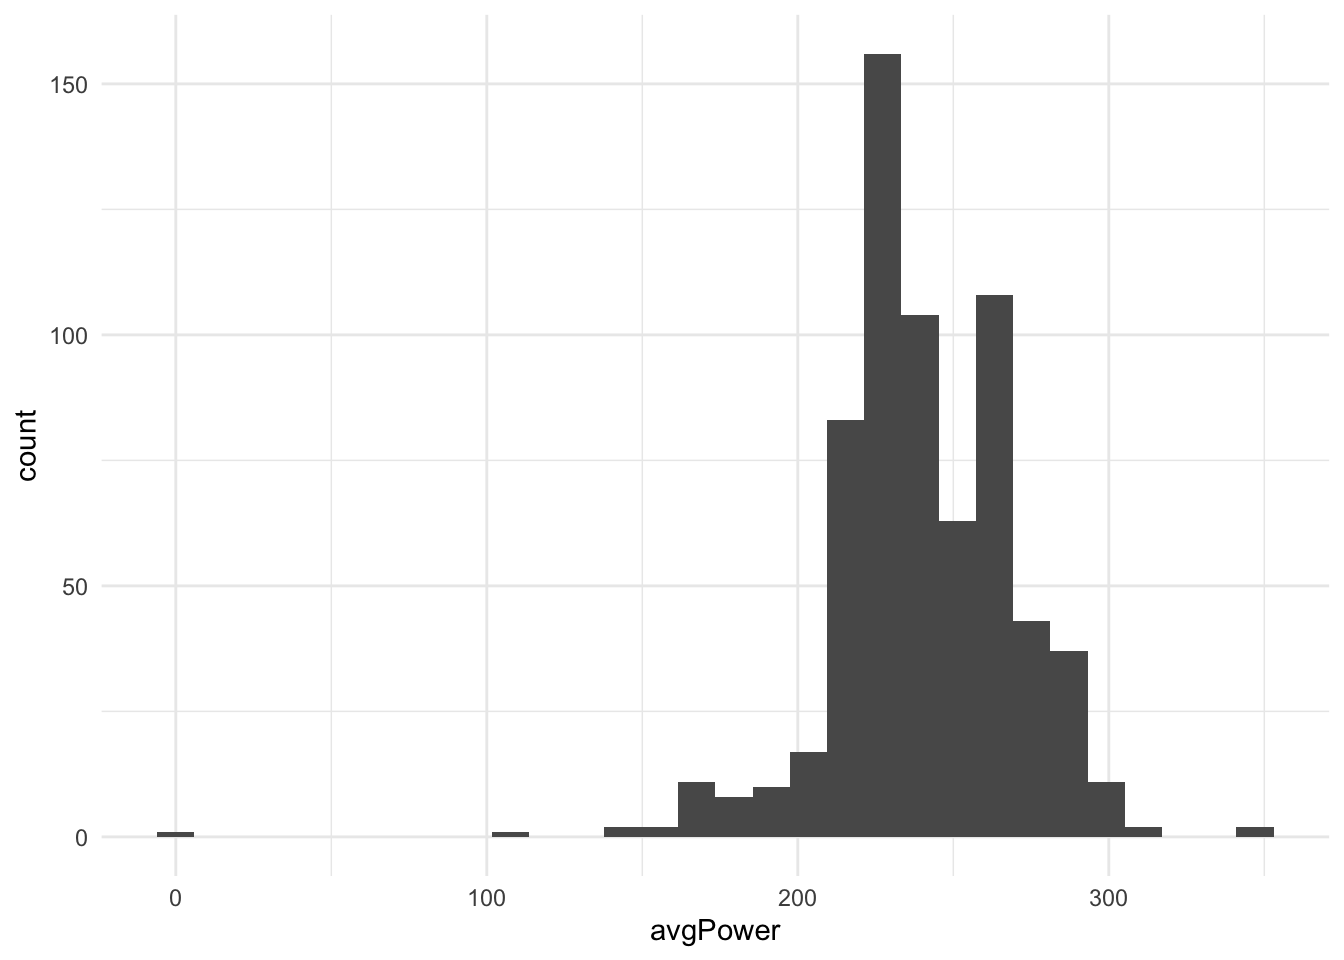
\includegraphics{DataExploration_files/figure-latex/unnamed-chunk-38-1.pdf}

\begin{Shaded}
\begin{Highlighting}[]
\KeywordTok{ggplot}\NormalTok{(dat,}\KeywordTok{aes}\NormalTok{(avgPower)) }\OperatorTok{+}\StringTok{ }\KeywordTok{geom_density}\NormalTok{() }\OperatorTok{+}\StringTok{ }\KeywordTok{theme_minimal}\NormalTok{()}
\end{Highlighting}
\end{Shaded}

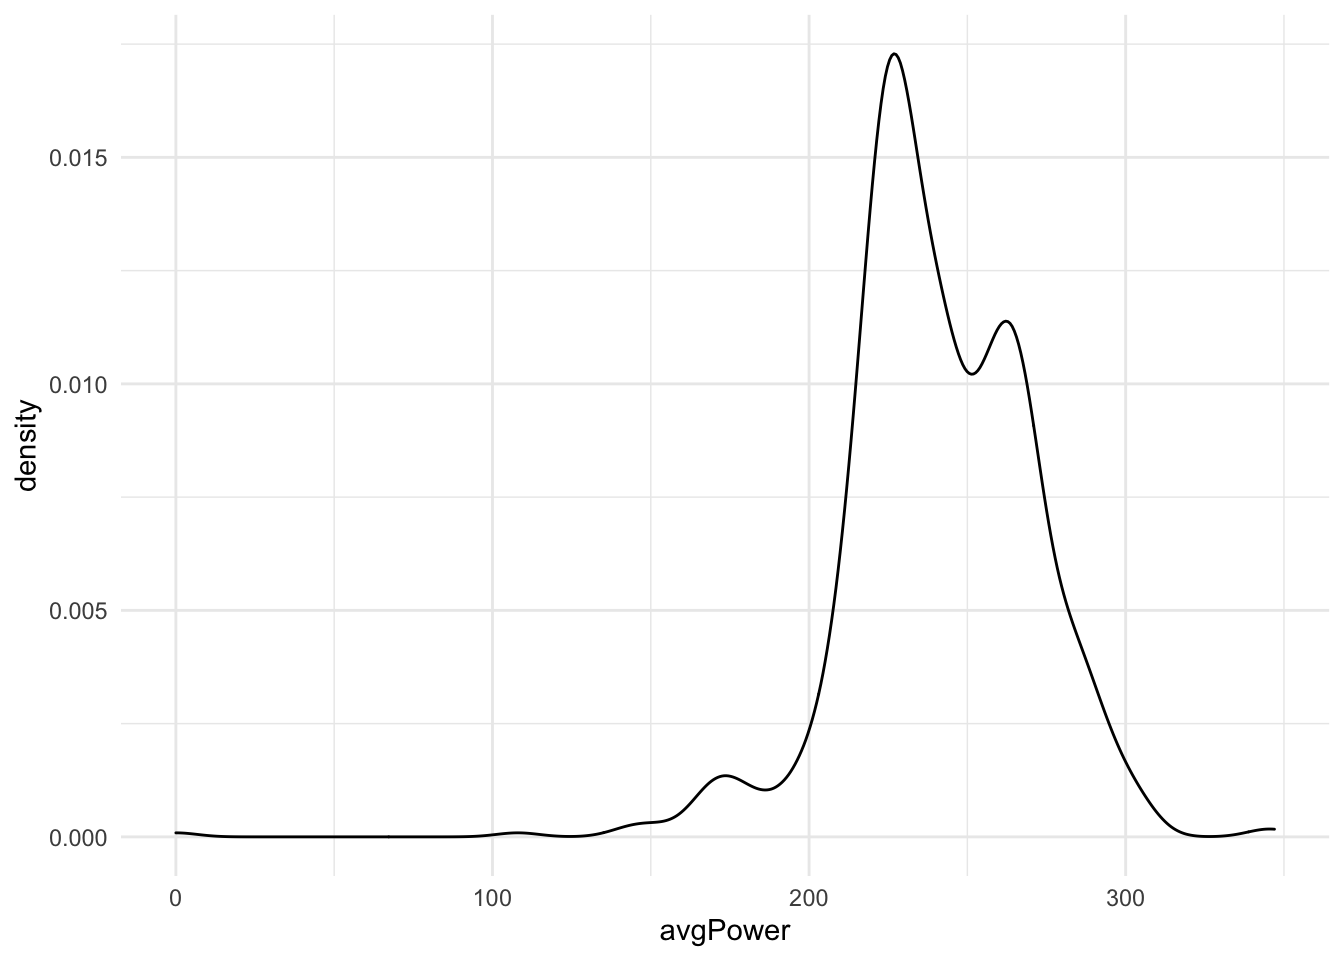
\includegraphics{DataExploration_files/figure-latex/unnamed-chunk-38-2.pdf}

\hypertarget{descriptive-statistics}{%
\subsubsection{Descriptive statistics}\label{descriptive-statistics}}

We typically want to measure what the ``average'' value is, along with ``how diverse is my population''. For that, we can use either sum-based statistics (mean, standard deviation) or quantiles.
Quantile-based statistics are said to be \textbf{robust} because much less sensitive to outliers. But they are more computationally expensive.

\begin{Shaded}
\begin{Highlighting}[]
\NormalTok{stats <-}\StringTok{ }\KeywordTok{c}\NormalTok{(}\KeywordTok{quantile}\NormalTok{(dat}\OperatorTok{$}\NormalTok{avgPower,}\DecValTok{1}\OperatorTok{:}\DecValTok{3}\OperatorTok{/}\DecValTok{4}\NormalTok{,}\DataTypeTok{na.rm =}\NormalTok{ T),}\KeywordTok{mean}\NormalTok{(dat}\OperatorTok{$}\NormalTok{avgPower,}\DataTypeTok{na.rm =}\NormalTok{ T))}
\KeywordTok{ggplot}\NormalTok{(dat,}\KeywordTok{aes}\NormalTok{(avgPower)) }\OperatorTok{+}\StringTok{ }\KeywordTok{geom_histogram}\NormalTok{() }\OperatorTok{+}
\StringTok{  }\KeywordTok{geom_vline}\NormalTok{(}\DataTypeTok{xintercept =}\NormalTok{ stats,}\DataTypeTok{color=}\StringTok{"red"}\NormalTok{) }\OperatorTok{+}\StringTok{ }
\StringTok{  }\KeywordTok{annotate}\NormalTok{(}\DataTypeTok{geom =} \StringTok{"text"}\NormalTok{,}\DataTypeTok{x=}\NormalTok{stats,}\DataTypeTok{y=}\KeywordTok{c}\NormalTok{(}\DecValTok{50}\NormalTok{,}\DecValTok{40}\NormalTok{,}\DecValTok{50}\NormalTok{,}\DecValTok{100}\NormalTok{),}\DataTypeTok{label=}\KeywordTok{c}\NormalTok{(}\StringTok{"Q1"}\NormalTok{,}\StringTok{"Q2=median"}\NormalTok{,}\StringTok{"Q3"}\NormalTok{,}\StringTok{"mean"}\NormalTok{),}\DataTypeTok{color=}\StringTok{"red"}\NormalTok{) }\OperatorTok{+}
\StringTok{  }\KeywordTok{geom_segment}\NormalTok{(}\KeywordTok{aes}\NormalTok{(}\DataTypeTok{x=}\DecValTok{200}\NormalTok{,}\DataTypeTok{y=}\DecValTok{25}\NormalTok{,}\DataTypeTok{xend=}\DecValTok{300}\NormalTok{,}\DataTypeTok{yend=}\DecValTok{25}\NormalTok{),}\DataTypeTok{color=}\StringTok{"blue"}\NormalTok{) }\OperatorTok{+}
\StringTok{  }\KeywordTok{annotate}\NormalTok{(}\DataTypeTok{geom=}\StringTok{"text"}\NormalTok{,}\DataTypeTok{x=}\DecValTok{300}\NormalTok{,}\DataTypeTok{y=}\DecValTok{30}\NormalTok{,}\DataTypeTok{label=}\StringTok{"dispersion"}\NormalTok{,}\DataTypeTok{color=}\StringTok{"blue"}\NormalTok{) }\OperatorTok{+}\StringTok{ }\KeywordTok{theme_minimal}\NormalTok{()}
\end{Highlighting}
\end{Shaded}

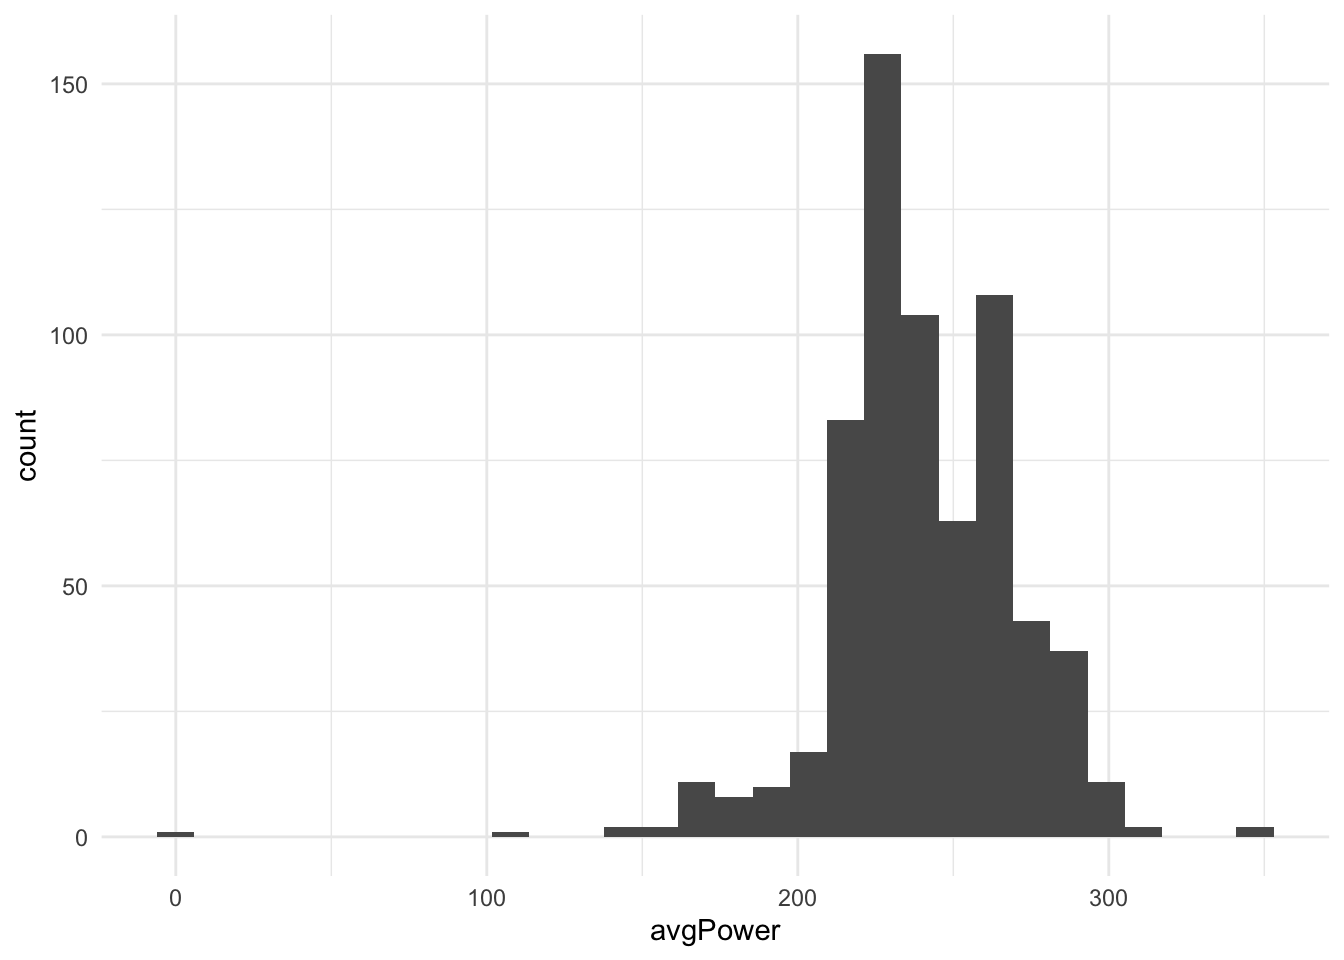
\includegraphics{DataExploration_files/figure-latex/unnamed-chunk-39-1.pdf}

\hypertarget{central-tendency}{%
\paragraph{Central tendency}\label{central-tendency}}

Central tendency statistics allow you to have an idea of the order of magnitude of the attribute you are interested in, over the population.

\begin{Shaded}
\begin{Highlighting}[]
\KeywordTok{summary}\NormalTok{(dat}\OperatorTok{$}\NormalTok{avgPower)}
\end{Highlighting}
\end{Shaded}

\begin{verbatim}
##    Min. 1st Qu.  Median    Mean 3rd Qu.    Max.    NA's 
##     0.0   224.0   239.0   240.6   261.0   347.0    4853
\end{verbatim}

\begin{Shaded}
\begin{Highlighting}[]
\KeywordTok{quantile}\NormalTok{(dat}\OperatorTok{$}\NormalTok{avgPower,}\DataTypeTok{probs=}\DecValTok{0}\OperatorTok{:}\DecValTok{10}\OperatorTok{/}\DecValTok{10}\NormalTok{,}\DataTypeTok{na.rm =}\NormalTok{ T)}
\end{Highlighting}
\end{Shaded}

\begin{verbatim}
##   0%  10%  20%  30%  40%  50%  60%  70%  80%  90% 100% 
##    0  212  221  226  230  239  246  258  265  276  347
\end{verbatim}

\hypertarget{dispersion}{%
\paragraph{Dispersion}\label{dispersion}}

Dispersion describes how heterogenous our population is. It can be measured with various measurements (not exhaustive here)

\begin{Shaded}
\begin{Highlighting}[]
\KeywordTok{sd}\NormalTok{(dat}\OperatorTok{$}\NormalTok{avgPower,}\DataTypeTok{na.rm =}\NormalTok{ T) }\CommentTok{# standard deviation}
\end{Highlighting}
\end{Shaded}

\begin{verbatim}
## [1] 29.83959
\end{verbatim}

\begin{Shaded}
\begin{Highlighting}[]
\KeywordTok{IQR}\NormalTok{(dat}\OperatorTok{$}\NormalTok{avgPower,}\DataTypeTok{na.rm =}\NormalTok{ T) }\CommentTok{# interquartile range}
\end{Highlighting}
\end{Shaded}

\begin{verbatim}
## [1] 37
\end{verbatim}

\begin{Shaded}
\begin{Highlighting}[]
\KeywordTok{sd}\NormalTok{(dat}\OperatorTok{$}\NormalTok{avgPower,}\DataTypeTok{na.rm =}\NormalTok{ T)}\OperatorTok{/}\KeywordTok{mean}\NormalTok{(dat}\OperatorTok{$}\NormalTok{avgPower,}\DataTypeTok{na.rm =}\NormalTok{ T) }\CommentTok{# coefficient of variation}
\end{Highlighting}
\end{Shaded}

\begin{verbatim}
## [1] 0.1240017
\end{verbatim}

How to read it :

\begin{itemize}
\tightlist
\item
  The average deviation to the average power is 29 watts
\item
  The age difference between the rides in the 25\% ``less powerful'' rides and the 25\% ``most powerful'' rides is 37 watts
\item
  The average deviation to the average power is 12\% of the average power
\end{itemize}

The latter allows to compare dispersion between variables that have different units

\hypertarget{dealing-with-various-shapes}{%
\subsubsection{Dealing with various shapes}\label{dealing-with-various-shapes}}

The traditional example of a distribution is the gaussian distribution

\begin{Shaded}
\begin{Highlighting}[]
\NormalTok{fake <-}\StringTok{ }\KeywordTok{data.frame}\NormalTok{(}\DataTypeTok{xx=}\KeywordTok{rnorm}\NormalTok{(}\DecValTok{100000}\NormalTok{,}\DecValTok{100}\NormalTok{,}\DecValTok{10}\NormalTok{))}
\KeywordTok{ggplot}\NormalTok{(fake,}\KeywordTok{aes}\NormalTok{(xx)) }\OperatorTok{+}\StringTok{ }\KeywordTok{geom_histogram}\NormalTok{() }\OperatorTok{+}\StringTok{ }\KeywordTok{labs}\NormalTok{(}\DataTypeTok{x=}\StringTok{"Random variable"}\NormalTok{)}\OperatorTok{+}\StringTok{ }\KeywordTok{theme_minimal}\NormalTok{()}
\end{Highlighting}
\end{Shaded}

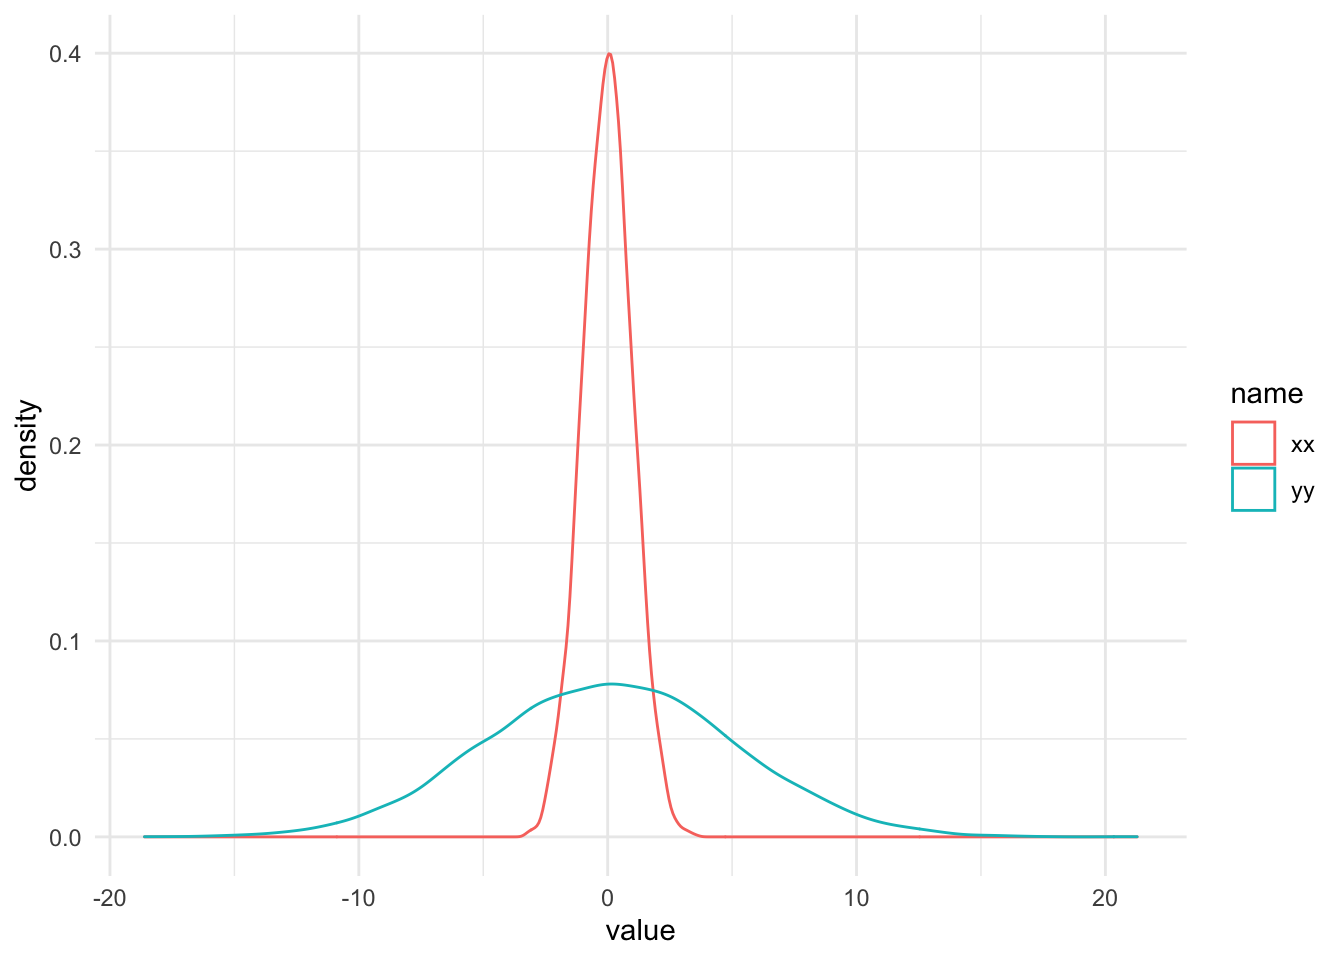
\includegraphics{DataExploration_files/figure-latex/unnamed-chunk-42-1.pdf}

In this case, we have a very interesting property : symmetry, which makes mean and median very close. If the coefficient of variation is not too high, the \textbf{tail} is pretty short.

In real life,it (almost) never happens. Therefore, to understand what happens, you can check :

\begin{itemize}
\tightlist
\item
  How different are mean and median
\item
  Does a log transformation make the distribution ``look better''
\item
  Is it symmetric \(\rightarrow\) skewness
\item
  Is flat no not \(\rightarrow\) kurtosis
\item
  Is the distribution highly concentrated (few individuals get almost the whole cake) \(\rightarrow\) concentration indexes (Gini, enthropy, Herfindahl\ldots). You can check the package \texttt{ineq}
\item
  Are there outliers (which generates a long tail) \(\rightarrow\) outlier detection (vast field\ldots). You can start with the previous
\end{itemize}

\textbf{Flat or not flat ?}

\begin{Shaded}
\begin{Highlighting}[]
\KeywordTok{data.frame}\NormalTok{(}\DataTypeTok{xx=}\KeywordTok{rnorm}\NormalTok{(}\DecValTok{10000}\NormalTok{),}\DataTypeTok{yy=}\KeywordTok{rnorm}\NormalTok{(}\DecValTok{10000}\NormalTok{,}\DecValTok{0}\NormalTok{,}\DecValTok{5}\NormalTok{))  }\OperatorTok\StringTok{ }
\StringTok{  }\KeywordTok{pivot_longer}\NormalTok{(}\KeywordTok{everything}\NormalTok{()) }\OperatorTok\StringTok{ }
\StringTok{  }\KeywordTok{ggplot}\NormalTok{(}\KeywordTok{aes}\NormalTok{(value,}\DataTypeTok{color=}\NormalTok{name)) }\OperatorTok{+}\StringTok{ }\KeywordTok{geom_density}\NormalTok{()}\OperatorTok{+}\StringTok{ }\KeywordTok{theme_minimal}\NormalTok{()}
\end{Highlighting}
\end{Shaded}

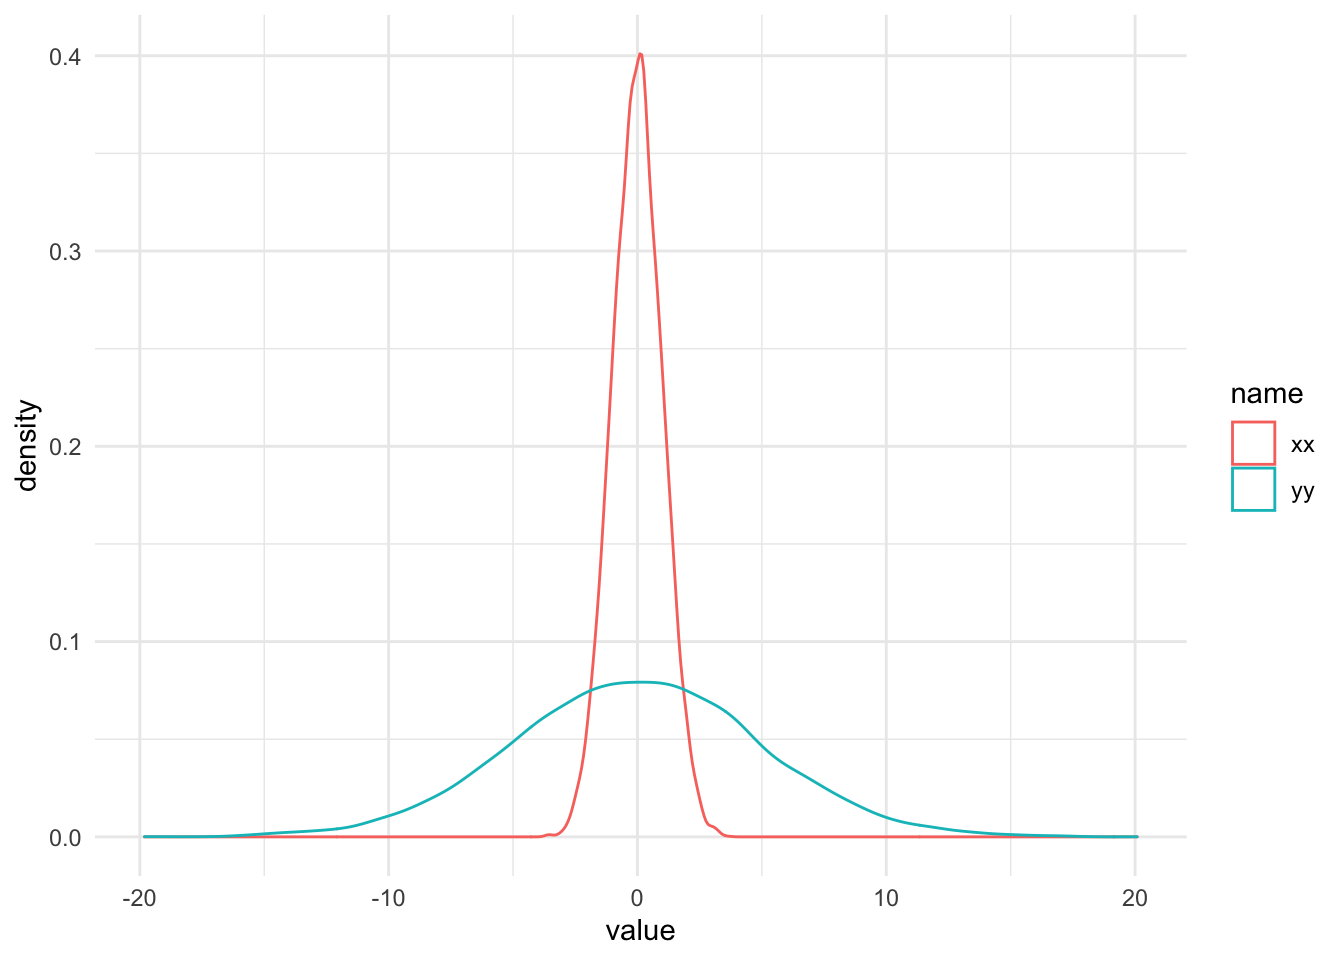
\includegraphics{DataExploration_files/figure-latex/unnamed-chunk-43-1.pdf}

\begin{Shaded}
\begin{Highlighting}[]
\KeywordTok{ggplot}\NormalTok{(dat,}\KeywordTok{aes}\NormalTok{(distance)) }\OperatorTok{+}\StringTok{ }\KeywordTok{geom_histogram}\NormalTok{() }\OperatorTok{+}\StringTok{ }\KeywordTok{theme_minimal}\NormalTok{()}
\end{Highlighting}
\end{Shaded}

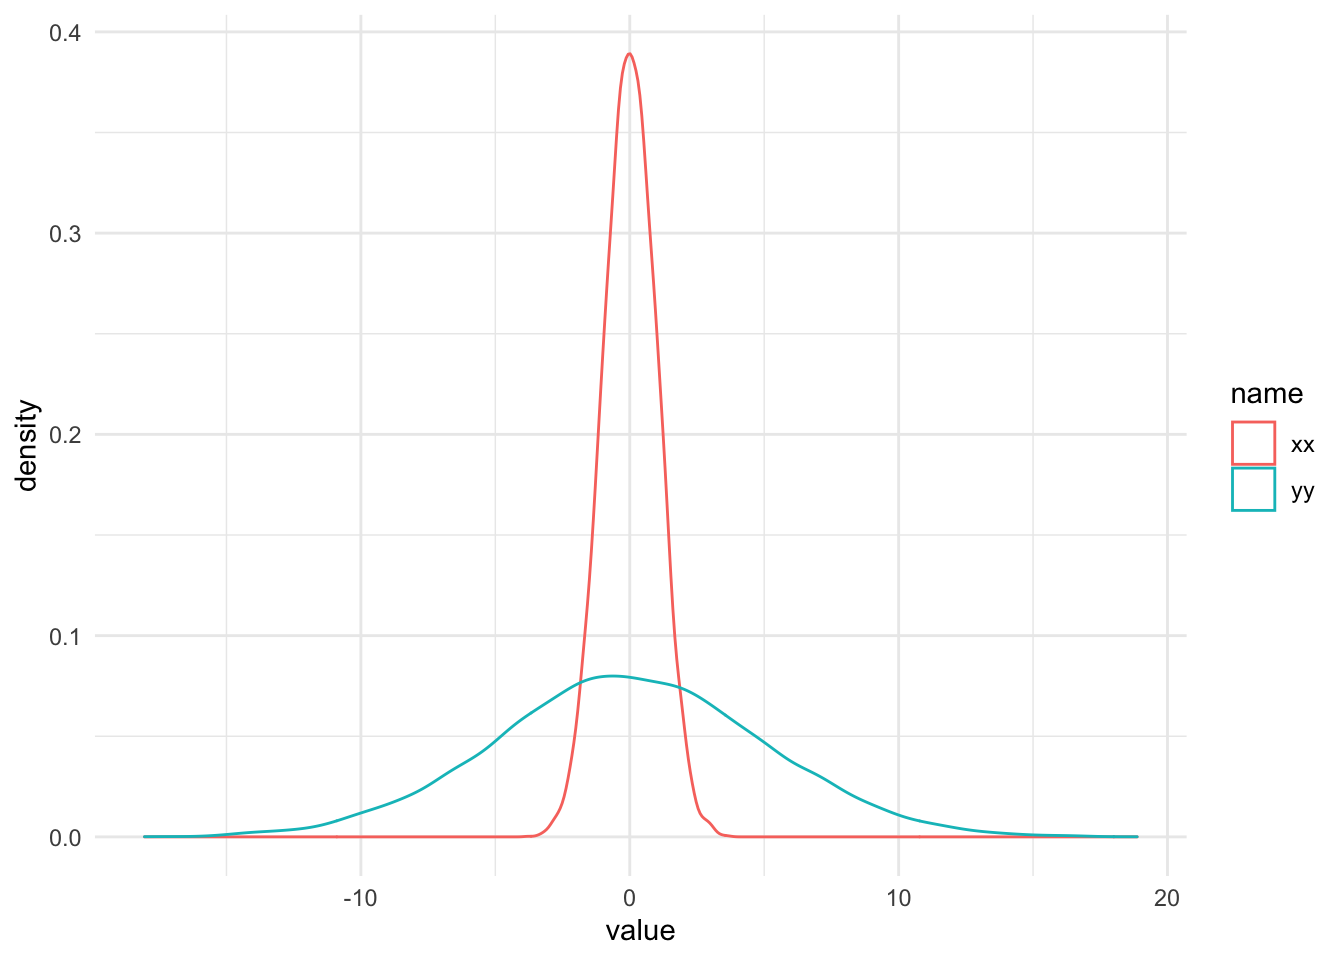
\includegraphics{DataExploration_files/figure-latex/unnamed-chunk-44-1.pdf}

\begin{Shaded}
\begin{Highlighting}[]
\KeywordTok{ggplot}\NormalTok{(dat,}\KeywordTok{aes}\NormalTok{(distance)) }\OperatorTok{+}\StringTok{ }\KeywordTok{geom_histogram}\NormalTok{() }\OperatorTok{+}\StringTok{ }\KeywordTok{scale_x_log10}\NormalTok{() }\OperatorTok{+}\StringTok{ }\KeywordTok{theme_minimal}\NormalTok{()}
\end{Highlighting}
\end{Shaded}

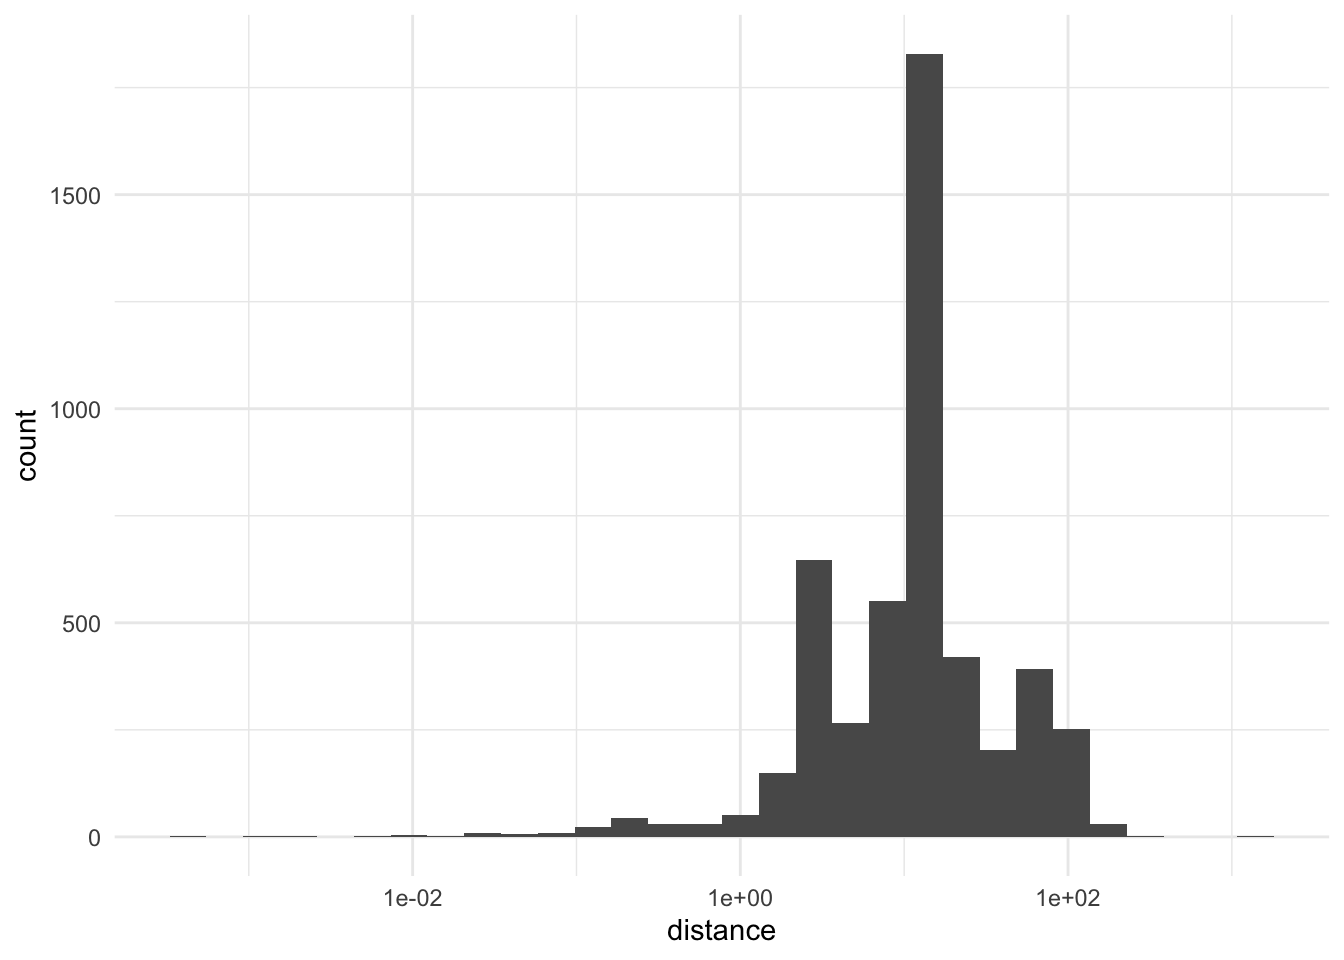
\includegraphics{DataExploration_files/figure-latex/unnamed-chunk-44-2.pdf}

\hypertarget{exercises}{%
\subsubsection{Exercises :}\label{exercises}}

What can you tell about the distance variable ?
- Draw the distribution of this variable. How much is the maximum distance of the 20\% shortest activities ; the minimum distance of the 5\% longest activities ?
- What unit do you think it is ? Did you check the maximum value ?
- Is there more dispersion in the distance or the average power ? using the \texttt{facet\_wrap} function of \texttt{ggplot2}, compare the distributions of distance and avgPower.
- I want to group activities in 5 categories based on the distance. This operation is called discretization (very useful for choropleth maps). Search for available methods, and apply some of them. Which one is best suited to this variable ? Which one should you avoid ?

\hypertarget{categorical-variables}{%
\subsection{Categorical variables}\label{categorical-variables}}

\hypertarget{working-with-factors}{%
\subsubsection{Working with factors}\label{working-with-factors}}

Factors are an optimized way to store categorical variables (encoded in integers). The distinct categories are stored in the \texttt{level} attribute which you can interact with.

\begin{Shaded}
\begin{Highlighting}[]
\KeywordTok{as.factor}\NormalTok{(dat}\OperatorTok{$}\NormalTok{activityType) }\OperatorTok\StringTok{ }
\StringTok{  }\KeywordTok{levels}\NormalTok{()}
\end{Highlighting}
\end{Shaded}

\begin{verbatim}
##  [1] "cross_country_skiing_ws" "cycling"                
##  [3] "cyclocross"              "hiking"                 
##  [5] "indoor_cardio"           "indoor_cycling"         
##  [7] "indoor_running"          "lap_swimming"           
##  [9] "multi_sport"             "open_water_swimming"    
## [11] "other"                   "road_biking"            
## [13] "running"                 "street_running"         
## [15] "strength_training"       "swimming"               
## [17] "swimToBikeTransition"    "trail_running"          
## [19] "transition"              "treadmill_running"      
## [21] "uncategorized"           "virtual_ride"           
## [23] "walking"
\end{verbatim}

\begin{Shaded}
\begin{Highlighting}[]
\KeywordTok{as.factor}\NormalTok{(dat}\OperatorTok{$}\NormalTok{activityType) }\OperatorTok\StringTok{ }
\StringTok{  }\KeywordTok{str}\NormalTok{()}
\end{Highlighting}
\end{Shaded}

\begin{verbatim}
##  Factor w/ 23 levels "cross_country_skiing_ws",..: 8 2 2 13 22 8 2 13 2 8 ...
\end{verbatim}

For more functionalities you can use the \href{https://cran.r-project.org/web/packages/forcats/vignettes/forcats.html}{forcats package} which provides convenient tools (eg to recode the variable)

\hypertarget{barcharts}{%
\subsubsection{Barcharts}\label{barcharts}}

The barchart (which IS NOT a histogram) is the most common representation for categorical variables. You can also use the pie chart (but it requires to hack a little ggplot).
Pie charts are despised by the majority of statisticians but it can be adapted if the sizes really differ. Some material to make your own opinion :

\begin{itemize}
\tightlist
\item
  \href{https://www.data-to-viz.com/caveat/pie.html}{Why it's bad}
\item
  \href{https://www.oreilly.com/content/in-defense-of-the-pie-chart/}{Defense}
\end{itemize}

\begin{Shaded}
\begin{Highlighting}[]
\KeywordTok{ggplot}\NormalTok{(dat,}\KeywordTok{aes}\NormalTok{(activityType)) }\OperatorTok{+}\StringTok{ }\KeywordTok{geom_bar}\NormalTok{() }\OperatorTok{+}\StringTok{ }\KeywordTok{coord_flip}\NormalTok{() }\OperatorTok{+}\StringTok{ }\KeywordTok{theme_minimal}\NormalTok{()}
\end{Highlighting}
\end{Shaded}

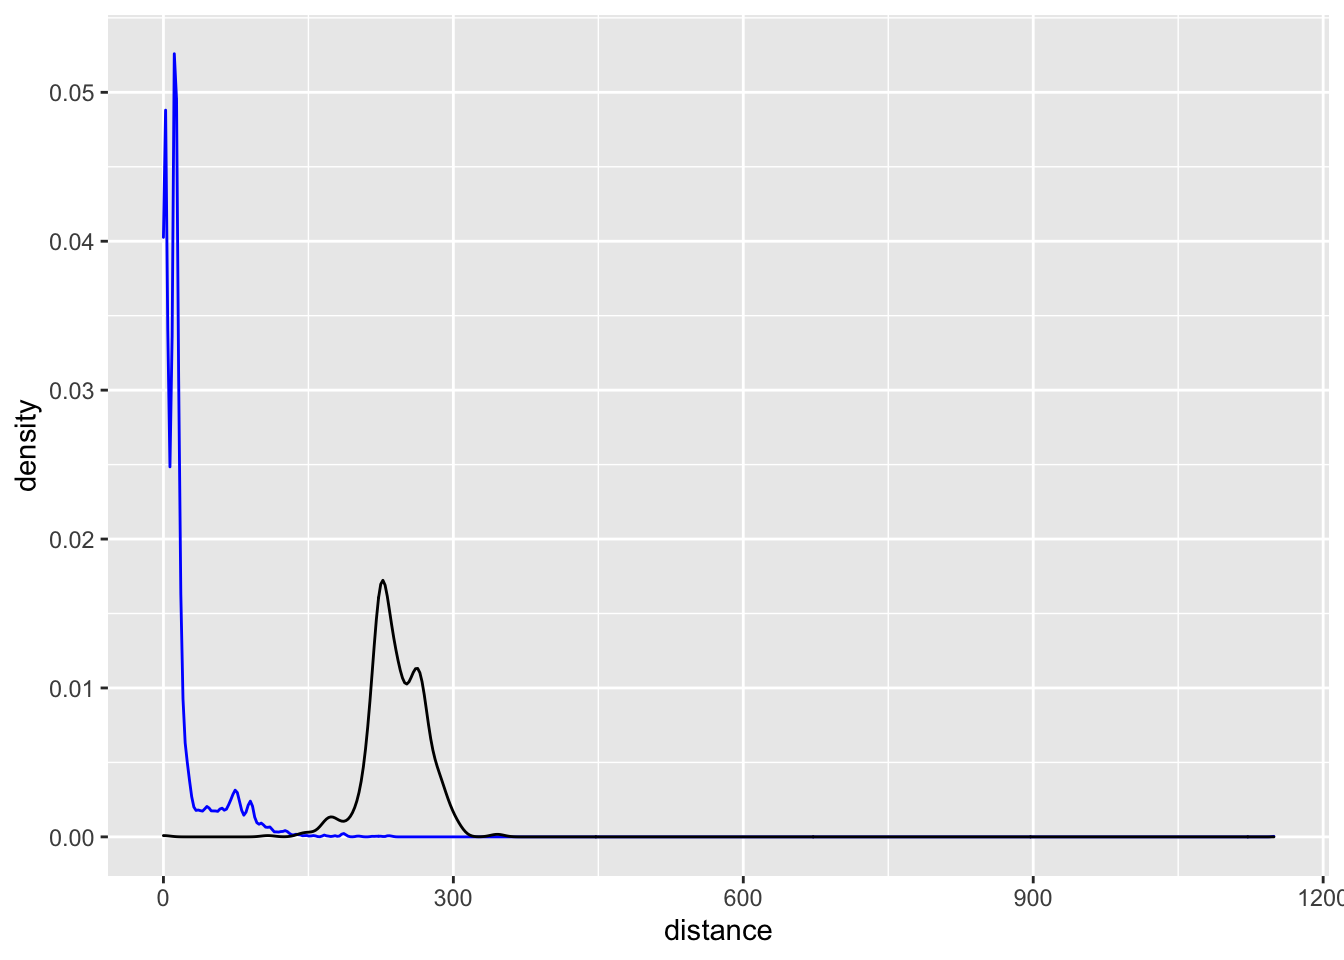
\includegraphics{DataExploration_files/figure-latex/unnamed-chunk-46-1.pdf}

\begin{Shaded}
\begin{Highlighting}[]
\KeywordTok{ggplot}\NormalTok{(dat,}\KeywordTok{aes}\NormalTok{(}\DataTypeTok{x=}\StringTok{""}\NormalTok{,}\DataTypeTok{fill=}\NormalTok{activityType)) }\OperatorTok{+}\StringTok{ }
\StringTok{  }\KeywordTok{geom_bar}\NormalTok{(}\DataTypeTok{width=}\DecValTok{1}\NormalTok{) }\OperatorTok{+}\StringTok{ }
\StringTok{  }\KeywordTok{coord_polar}\NormalTok{(}\StringTok{"y"}\NormalTok{,}\DataTypeTok{start=}\DecValTok{0}\NormalTok{) }\OperatorTok{+}\StringTok{ }
\StringTok{  }\KeywordTok{theme_void}\NormalTok{()}
\end{Highlighting}
\end{Shaded}

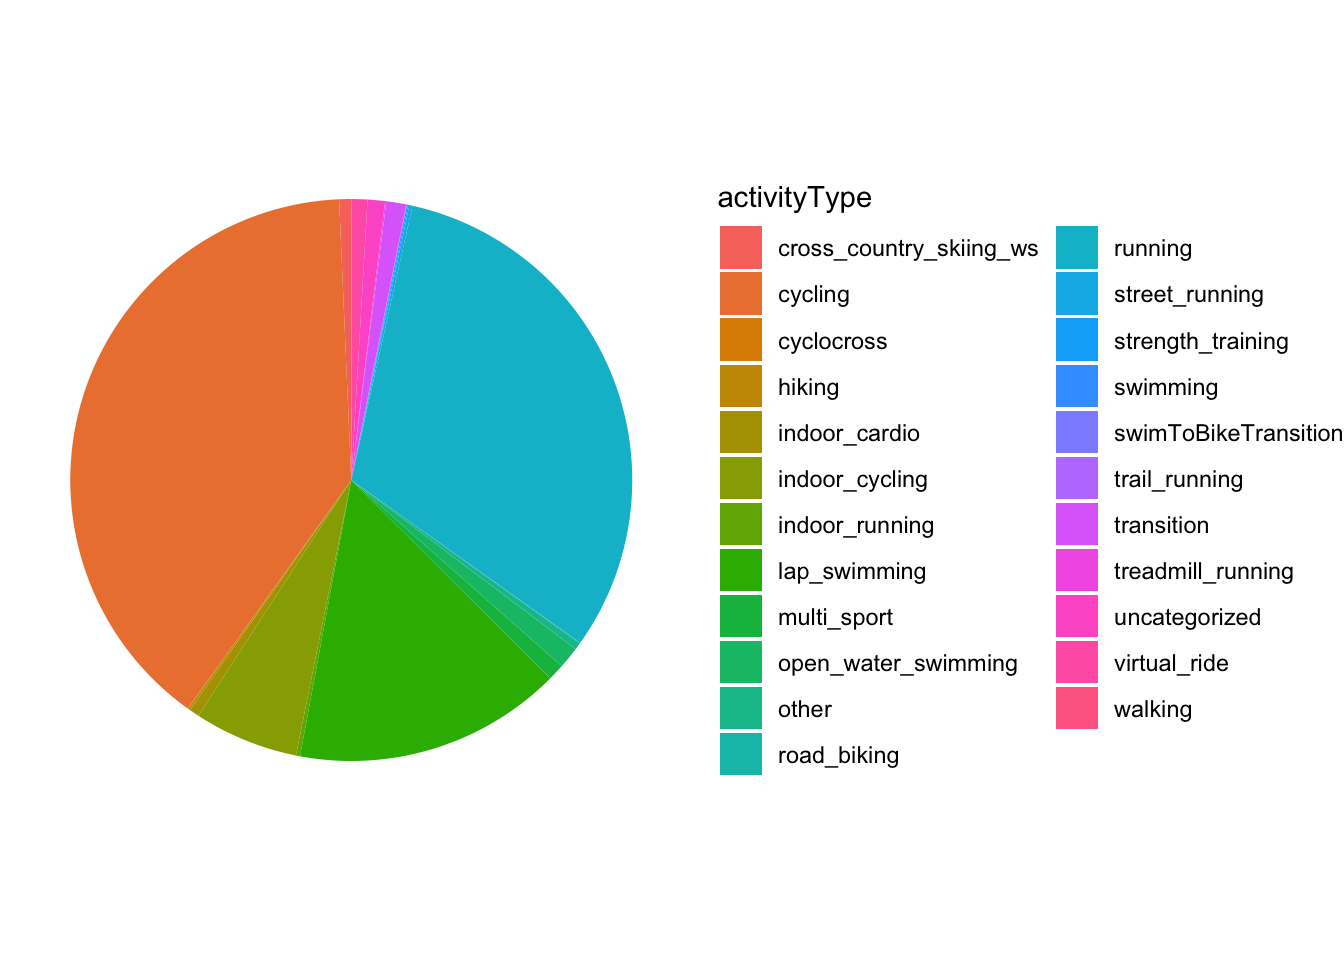
\includegraphics{DataExploration_files/figure-latex/unnamed-chunk-46-2.pdf}

\hypertarget{contingency-tables}{%
\subsubsection{Contingency tables}\label{contingency-tables}}

After visualizing, how can we measure the number of cases and the percent in each category ?

\begin{Shaded}
\begin{Highlighting}[]
\KeywordTok{table}\NormalTok{(dat}\OperatorTok{$}\NormalTok{activityType)}
\end{Highlighting}
\end{Shaded}

\begin{verbatim}
## 
## cross_country_skiing_ws                 cycling              cyclocross 
##                      38                    2174                       1 
##                  hiking           indoor_cardio          indoor_cycling 
##                       7                      32                     331 
##          indoor_running            lap_swimming             multi_sport 
##                      13                     852                      52 
##     open_water_swimming                   other             road_biking 
##                      69                      22                       2 
##                 running          street_running       strength_training 
##                    1728                      10                       4 
##                swimming    swimToBikeTransition           trail_running 
##                       4                       1                       1 
##              transition       treadmill_running           uncategorized 
##                      63                       4                      55 
##            virtual_ride                 walking 
##                      49                       2
\end{verbatim}

\begin{Shaded}
\begin{Highlighting}[]
\KeywordTok{table}\NormalTok{(dat}\OperatorTok{$}\NormalTok{activityType) }\OperatorTok\StringTok{ }
\StringTok{  }\KeywordTok{prop.table}\NormalTok{()}\OperatorTok{*}\DecValTok{100} 
\end{Highlighting}
\end{Shaded}

\begin{verbatim}
## 
## cross_country_skiing_ws                 cycling              cyclocross 
##              0.68915488             39.42691331              0.01813565 
##                  hiking           indoor_cardio          indoor_cycling 
##              0.12694958              0.58034095              6.00290170 
##          indoor_running            lap_swimming             multi_sport 
##              0.23576351             15.45157780              0.94305404 
##     open_water_swimming                   other             road_biking 
##              1.25136017              0.39898440              0.03627131 
##                 running          street_running       strength_training 
##             31.33841132              0.18135655              0.07254262 
##                swimming    swimToBikeTransition           trail_running 
##              0.07254262              0.01813565              0.01813565 
##              transition       treadmill_running           uncategorized 
##              1.14254625              0.07254262              0.99746101 
##            virtual_ride                 walking 
##              0.88864708              0.03627131
\end{verbatim}

Another solution is to use what you've learned in the previous section (@ref()) : aggregation !

\begin{Shaded}
\begin{Highlighting}[]
\KeywordTok{group_by}\NormalTok{(dat,activityType) }\OperatorTok\StringTok{ }
\StringTok{  }\KeywordTok{summarise}\NormalTok{(}\DataTypeTok{number=}\KeywordTok{n}\NormalTok{(),}\DataTypeTok{proportion=}\KeywordTok{n}\NormalTok{()}\OperatorTok{/}\KeywordTok{nrow}\NormalTok{(dat))}
\end{Highlighting}
\end{Shaded}

\begin{verbatim}
## # A tibble: 23 x 3
##    activityType            number proportion
##    <chr>                    <int>      <dbl>
##  1 cross_country_skiing_ws     38   0.00689 
##  2 cycling                   2174   0.394   
##  3 cyclocross                   1   0.000181
##  4 hiking                       7   0.00127 
##  5 indoor_cardio               32   0.00580 
##  6 indoor_cycling             331   0.0600  
##  7 indoor_running              13   0.00236 
##  8 lap_swimming               852   0.155   
##  9 multi_sport                 52   0.00943 
## 10 open_water_swimming         69   0.0125  
## # ... with 13 more rows
\end{verbatim}

\hypertarget{bivariate-statistics}{%
\section{Bivariate statistics}\label{bivariate-statistics}}

In this section, we see how to represent the relationship between two variables and measure it

\hypertarget{continuous-variables}{%
\subsection{2 continuous variables}\label{continuous-variables}}

\hypertarget{graphical-exploration}{%
\subsubsection{Graphical exploration}\label{graphical-exploration}}

To visualize the relationship between two numerical variables, we can use the scatter plot. Don't forget that the log function can help you identify non linear relationships since \(log(a \cdot x^b) = log(a) + b \cdot log(x)\)

\begin{Shaded}
\begin{Highlighting}[]
\KeywordTok{ggplot}\NormalTok{(dat,}\KeywordTok{aes}\NormalTok{(distance,avgPower)) }\OperatorTok{+}\StringTok{ }\KeywordTok{geom_jitter}\NormalTok{() }\OperatorTok{+}\StringTok{ }
\StringTok{  }\KeywordTok{labs}\NormalTok{(}\DataTypeTok{x=}\StringTok{"Distance"}\NormalTok{,}\DataTypeTok{y=}\StringTok{"Power"}\NormalTok{,}\DataTypeTok{title=}\StringTok{"Raw variables"}\NormalTok{) }\OperatorTok{+}\StringTok{ }\KeywordTok{scale_x_continuous}\NormalTok{(}\DataTypeTok{labels =}\NormalTok{ scales}\OperatorTok{::}\NormalTok{comma)}\OperatorTok{+}\StringTok{ }\KeywordTok{theme_minimal}\NormalTok{()}
\end{Highlighting}
\end{Shaded}

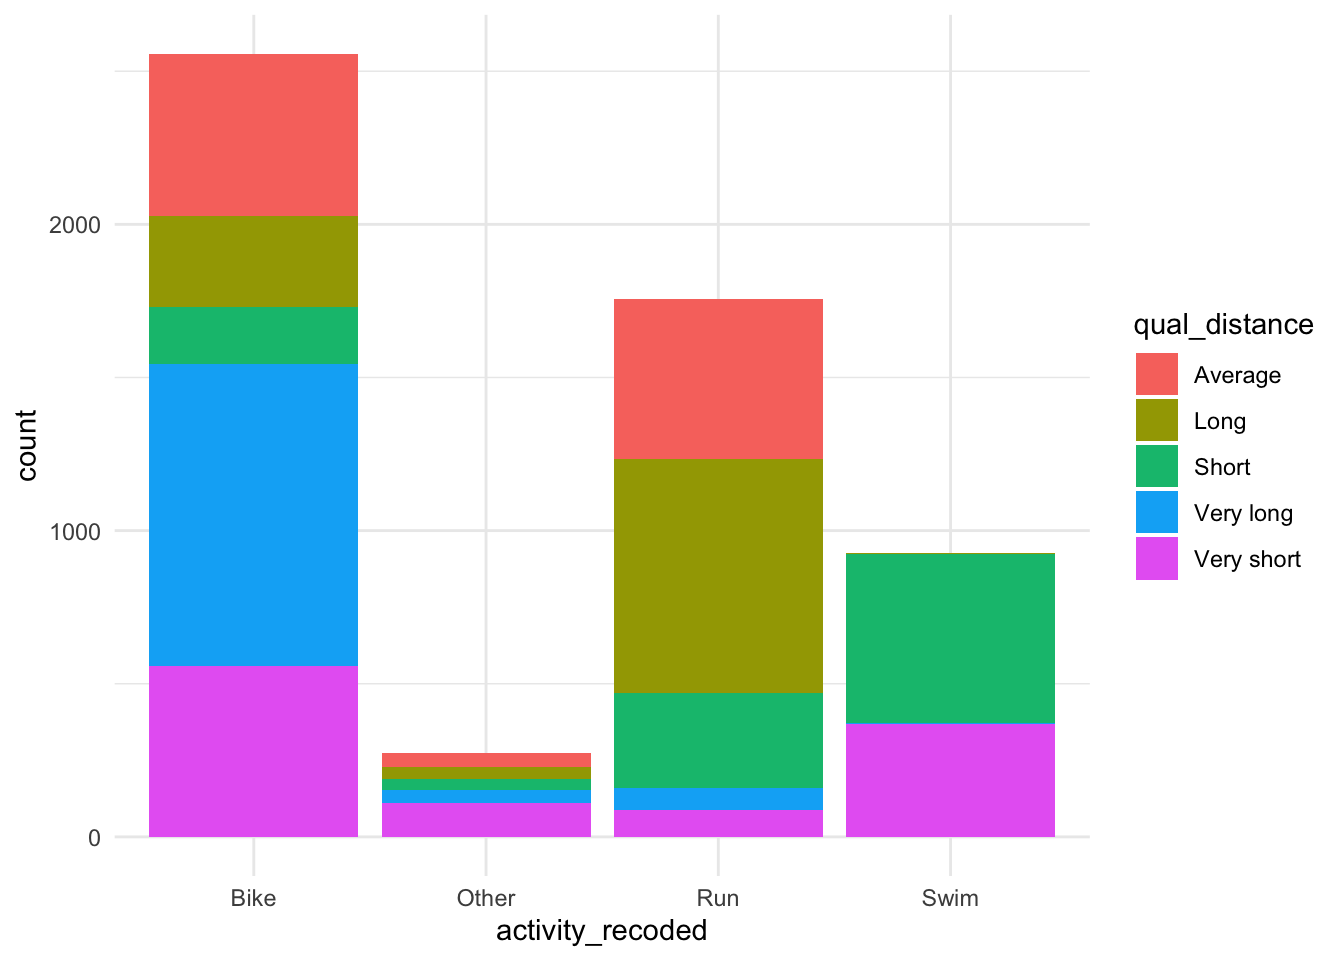
\includegraphics{DataExploration_files/figure-latex/unnamed-chunk-49-1.pdf}

\begin{Shaded}
\begin{Highlighting}[]
\KeywordTok{ggplot}\NormalTok{(dat,}\KeywordTok{aes}\NormalTok{(distance,avgPower)) }\OperatorTok{+}\StringTok{ }\KeywordTok{geom_jitter}\NormalTok{() }\OperatorTok{+}\StringTok{ }\KeywordTok{scale_x_log10}\NormalTok{(}\DataTypeTok{labels =}\NormalTok{ scales}\OperatorTok{::}\NormalTok{comma) }\OperatorTok{+}\StringTok{ }
\StringTok{  }\KeywordTok{labs}\NormalTok{(}\DataTypeTok{x=}\StringTok{"Distance"}\NormalTok{,}\DataTypeTok{y=}\StringTok{"Power"}\NormalTok{,}\DataTypeTok{title=}\StringTok{"Distance in log scale"}\NormalTok{) }\OperatorTok{+}\StringTok{ }\KeywordTok{theme_minimal}\NormalTok{()}
\end{Highlighting}
\end{Shaded}

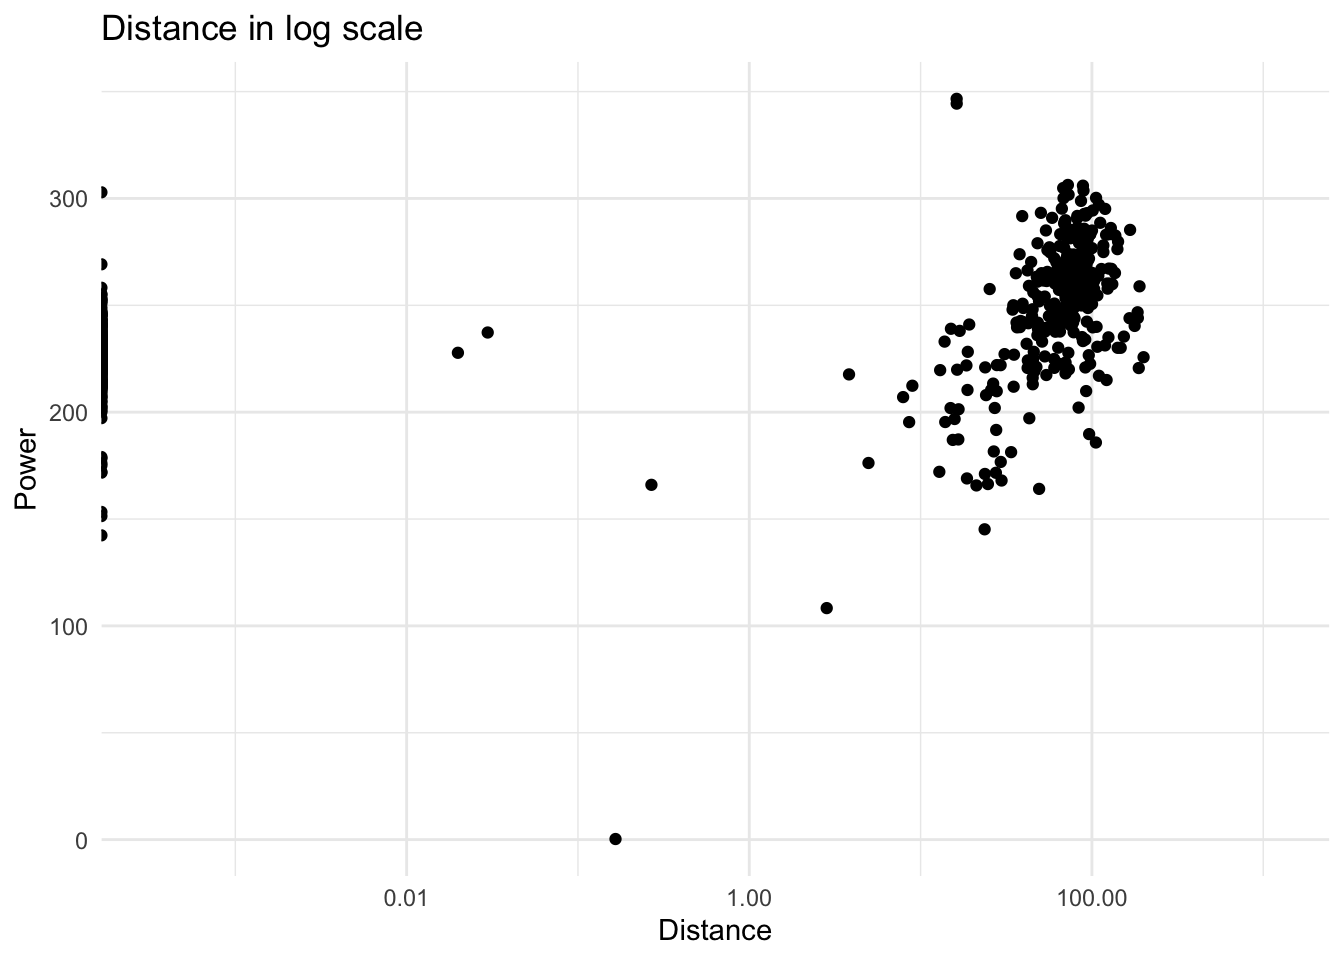
\includegraphics{DataExploration_files/figure-latex/unnamed-chunk-49-2.pdf}

We can pimp up the graphics a bit to visualize the correlation

\begin{Shaded}
\begin{Highlighting}[]
\KeywordTok{ggplot}\NormalTok{(dat,}\KeywordTok{aes}\NormalTok{(distance}\OperatorTok{/}\FloatTok{1E5}\NormalTok{,avgPower)) }\OperatorTok{+}\StringTok{ }\KeywordTok{geom_jitter}\NormalTok{() }\OperatorTok{+}\StringTok{ }\KeywordTok{scale_x_log10}\NormalTok{(}\DataTypeTok{labels =}\NormalTok{ scales}\OperatorTok{::}\NormalTok{comma) }\OperatorTok{+}\StringTok{ }
\StringTok{  }\KeywordTok{labs}\NormalTok{(}\DataTypeTok{x=}\StringTok{"Distance"}\NormalTok{,}\DataTypeTok{y=}\StringTok{"Power"}\NormalTok{,}\DataTypeTok{title=}\StringTok{"Usage in log scale"}\NormalTok{)}\OperatorTok{+}\StringTok{  }\KeywordTok{geom_smooth}\NormalTok{(}\DataTypeTok{method=}\StringTok{"lm"}\NormalTok{) }\OperatorTok{+}\StringTok{ }\KeywordTok{theme_minimal}\NormalTok{()}
\end{Highlighting}
\end{Shaded}

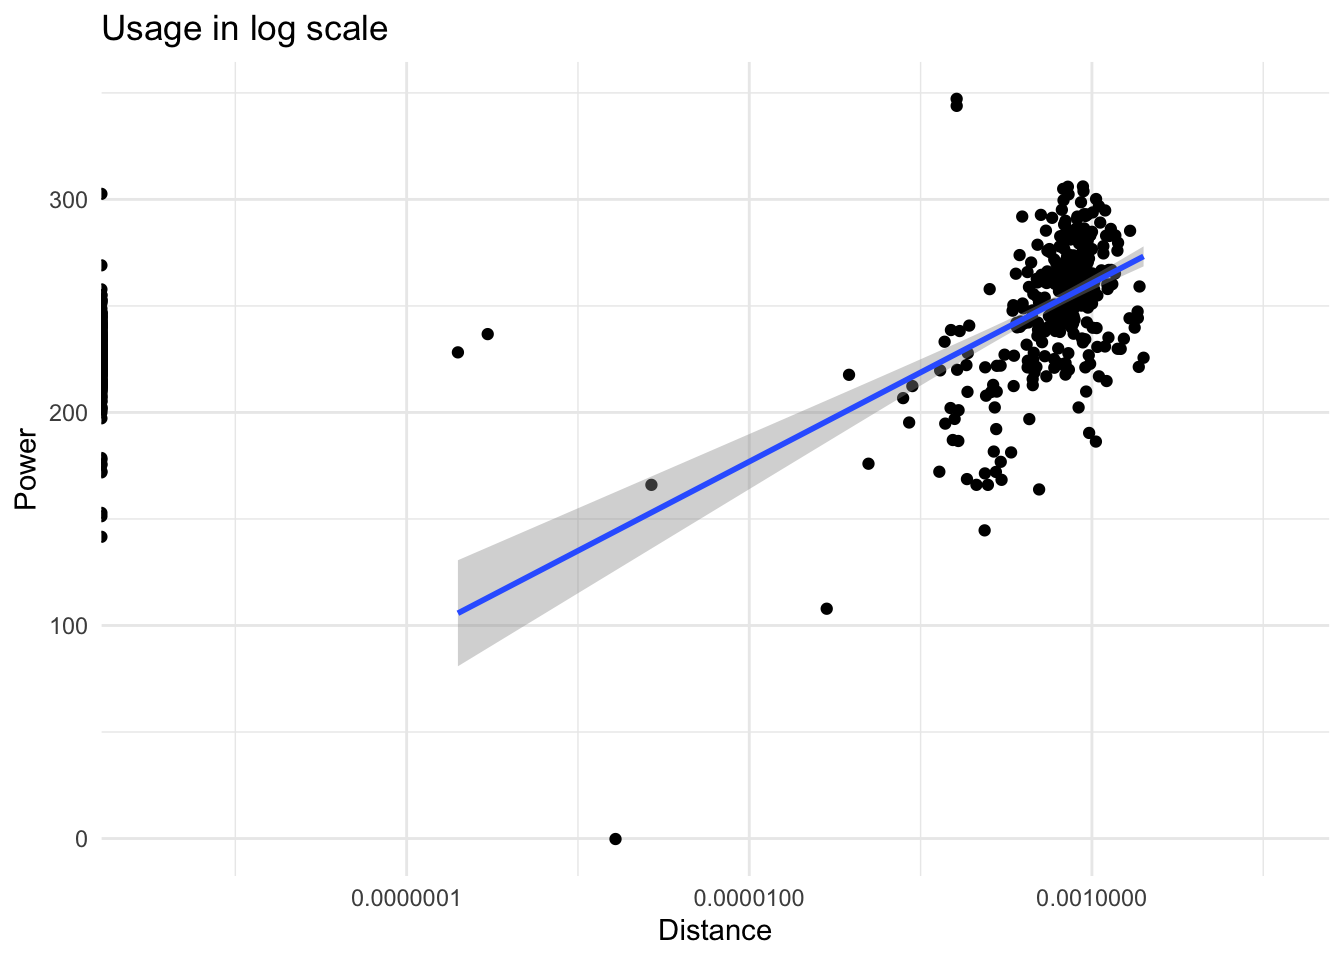
\includegraphics{DataExploration_files/figure-latex/unnamed-chunk-50-1.pdf}

We can see here that there is a positive relationship between distance and data usage and that this relationship has an exponential shape, meaning that the usage increases A LOT when the age drops.

\hypertarget{quantifying-the-relationship-correlations}{%
\subsubsection{\texorpdfstring{Quantifying the relationship : correlation\textbf{s}}{Quantifying the relationship : correlations}}\label{quantifying-the-relationship-correlations}}

To quantify this relationship, you can use the coefficients of correlation. There are 3 main coefficients : Pearson (the most famous and used), Kendall and Spearman. The latter can handle non-linear functional dependencies (ranks correlation) ; this is (roughly) equivalent to computing the coefficients on the log-transformed variables.

\begin{Shaded}
\begin{Highlighting}[]
\CommentTok{# Pearson coeff}
\KeywordTok{cor}\NormalTok{(dat}\OperatorTok{$}\NormalTok{distance,dat}\OperatorTok{$}\NormalTok{avgPower,}\DataTypeTok{method=}\StringTok{"pearson"}\NormalTok{)}
\end{Highlighting}
\end{Shaded}

\begin{verbatim}
## [1] NA
\end{verbatim}

\begin{Shaded}
\begin{Highlighting}[]
\CommentTok{# Pearson coeff, NAs removed}
\KeywordTok{cor}\NormalTok{(dat}\OperatorTok{$}\NormalTok{distance,dat}\OperatorTok{$}\NormalTok{avgPower,}\DataTypeTok{method=}\StringTok{"pearson"}\NormalTok{,}\DataTypeTok{use =} \StringTok{"complete.obs"}\NormalTok{)}
\end{Highlighting}
\end{Shaded}

\begin{verbatim}
## [1] 0.5437859
\end{verbatim}

\begin{Shaded}
\begin{Highlighting}[]
\CommentTok{# Spearman coeff }
\KeywordTok{cor}\NormalTok{(dat}\OperatorTok{$}\NormalTok{distance,dat}\OperatorTok{$}\NormalTok{avgPower,}\DataTypeTok{method=}\StringTok{"spearman"}\NormalTok{,}\DataTypeTok{use =} \StringTok{"complete.obs"}\NormalTok{)}
\end{Highlighting}
\end{Shaded}

\begin{verbatim}
## [1] 0.6316721
\end{verbatim}

\begin{Shaded}
\begin{Highlighting}[]
\CommentTok{# Why is R a beautiful language ? Do it at once, without loops (loops are evil) }
\KeywordTok{print}\NormalTok{(}\StringTok{"all coeffs"}\NormalTok{)}
\end{Highlighting}
\end{Shaded}

\begin{verbatim}
## [1] "all coeffs"
\end{verbatim}

\begin{Shaded}
\begin{Highlighting}[]
\KeywordTok{sapply}\NormalTok{(}\KeywordTok{c}\NormalTok{(}\StringTok{"pearson"}\NormalTok{,}\StringTok{"spearman"}\NormalTok{,}\StringTok{"kendall"}\NormalTok{),}\ControlFlowTok{function}\NormalTok{(xx) }\KeywordTok{cor}\NormalTok{(dat}\OperatorTok{$}\NormalTok{distance,dat}\OperatorTok{$}\NormalTok{avgPower,}\DataTypeTok{method=}\NormalTok{xx,}\DataTypeTok{use =} \StringTok{"complete.obs"}\NormalTok{))}
\end{Highlighting}
\end{Shaded}

\begin{verbatim}
##   pearson  spearman   kendall 
## 0.5437859 0.6316721 0.4452121
\end{verbatim}

More \href{https://www.statisticssolutions.com/correlation-pearson-kendall-spearman/}{info about correlation coefficients}

Should there be a complex relationship (eg sine), the graphical exploration is mandatory !

\hypertarget{categorical-variables-1}{%
\subsection{2 categorical variables}\label{categorical-variables-1}}

For this part, I will create a discrete variable out of the distance variable (see previous exercises) to use it as second qualitative variable (the other ones are not really meaningful)

\begin{Shaded}
\begin{Highlighting}[]
\NormalTok{dat <-}\StringTok{ }\KeywordTok{mutate}\NormalTok{(dat,}\DataTypeTok{qual_distance=}\KeywordTok{as.character}\NormalTok{(}\KeywordTok{cut}\NormalTok{(distance,}
                                                 \KeywordTok{quantile}\NormalTok{(distance,}\DataTypeTok{probs =} \DecValTok{0}\OperatorTok{:}\DecValTok{5}\OperatorTok{/}\DecValTok{5}\NormalTok{,}\DataTypeTok{na.rm=}\NormalTok{T),}
                                                 \DataTypeTok{include.lowest =}\NormalTok{ T,}
                                                 \DataTypeTok{labels=}\KeywordTok{c}\NormalTok{(}\StringTok{"Very short"}\NormalTok{,}\StringTok{"Short"}\NormalTok{,}
                                                          \StringTok{"Average"}\NormalTok{,}\StringTok{"Long"}\NormalTok{,}\StringTok{"Very long"}\NormalTok{))),}
              \DataTypeTok{qual_avgHr=}\KeywordTok{as.character}\NormalTok{(}\KeywordTok{cut}\NormalTok{(avgHr,}\KeywordTok{quantile}\NormalTok{(avgHr,}\DecValTok{0}\OperatorTok{:}\DecValTok{3}\OperatorTok{/}\DecValTok{5}\NormalTok{,}\DataTypeTok{na.rm =}\NormalTok{ T),}
                                          \DataTypeTok{include.lowest =}\NormalTok{ T,}
                                          \DataTypeTok{labels=}\KeywordTok{c}\NormalTok{(}\StringTok{"Low intensity"}\NormalTok{,}\StringTok{"Average intensity"}\NormalTok{,}
                                                   \StringTok{"High intensity"}\NormalTok{))),}
              \DataTypeTok{qual_distance=}\KeywordTok{ifelse}\NormalTok{(}\KeywordTok{is.na}\NormalTok{(qual_distance),}\StringTok{"Very short"}\NormalTok{,qual_distance))}
\end{Highlighting}
\end{Shaded}

Try different layouts with you barcharts !

\hypertarget{barcharts-1}{%
\subsubsection{Barcharts}\label{barcharts-1}}

\begin{Shaded}
\begin{Highlighting}[]
\KeywordTok{ggplot}\NormalTok{(dat,}\KeywordTok{aes}\NormalTok{(activity_recoded,}\DataTypeTok{fill=}\NormalTok{qual_distance)) }\OperatorTok{+}\StringTok{ }
\StringTok{  }\KeywordTok{geom_bar}\NormalTok{(}\DataTypeTok{position =} \StringTok{"stack"}\NormalTok{) }\OperatorTok{+}\StringTok{ }\KeywordTok{theme_minimal}\NormalTok{()}
\end{Highlighting}
\end{Shaded}

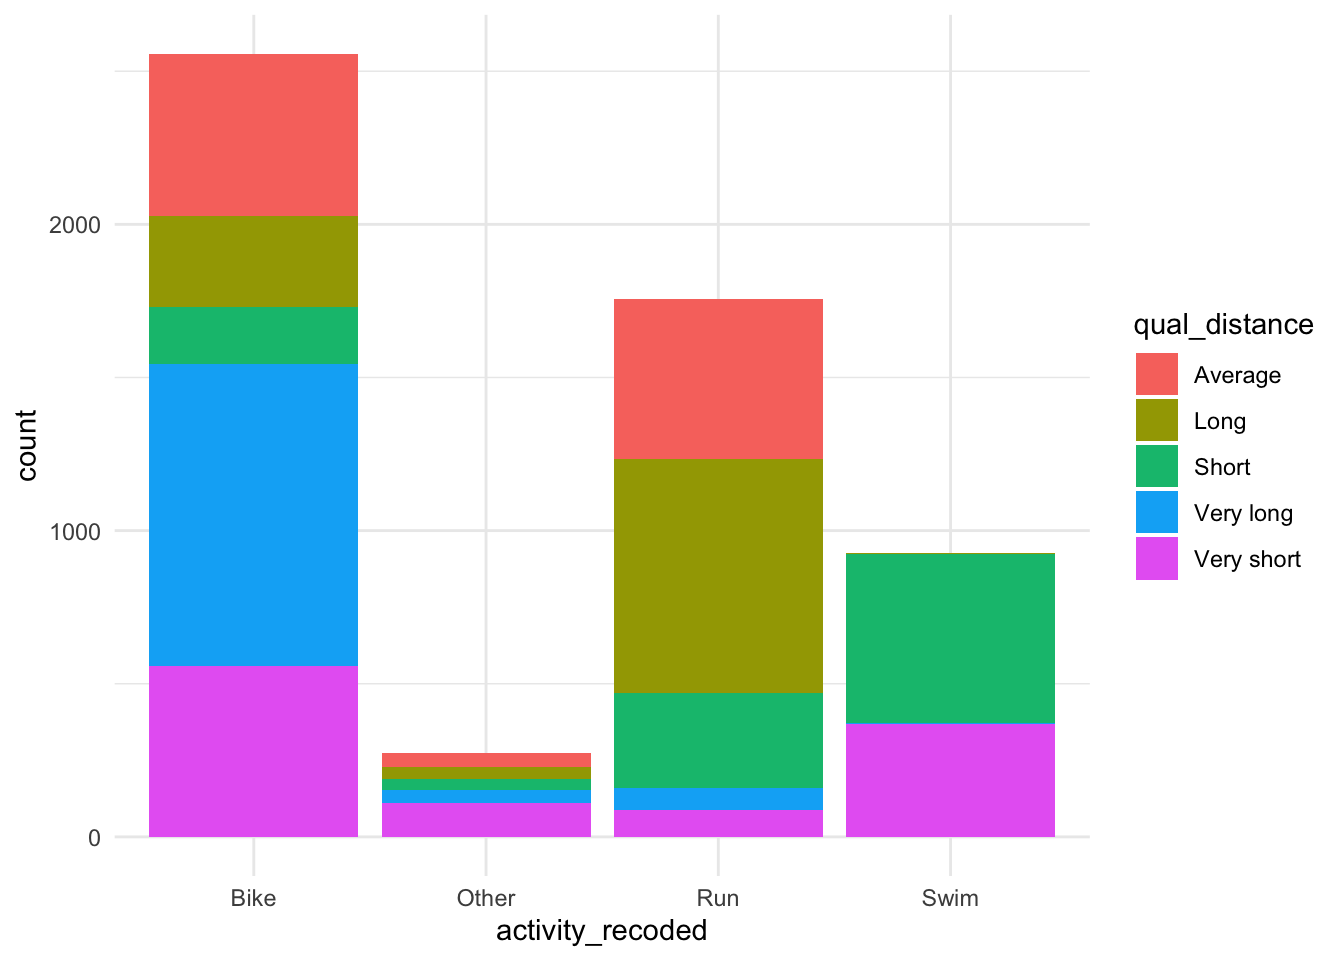
\includegraphics{DataExploration_files/figure-latex/unnamed-chunk-53-1.pdf}

\begin{Shaded}
\begin{Highlighting}[]
\KeywordTok{ggplot}\NormalTok{(dat,}\KeywordTok{aes}\NormalTok{(activity_recoded,}\DataTypeTok{fill=}\NormalTok{qual_distance)) }\OperatorTok{+}\StringTok{ }
\StringTok{  }\KeywordTok{geom_bar}\NormalTok{(}\DataTypeTok{position =} \StringTok{"dodge"}\NormalTok{) }\OperatorTok{+}\StringTok{ }\KeywordTok{theme_minimal}\NormalTok{()}
\end{Highlighting}
\end{Shaded}

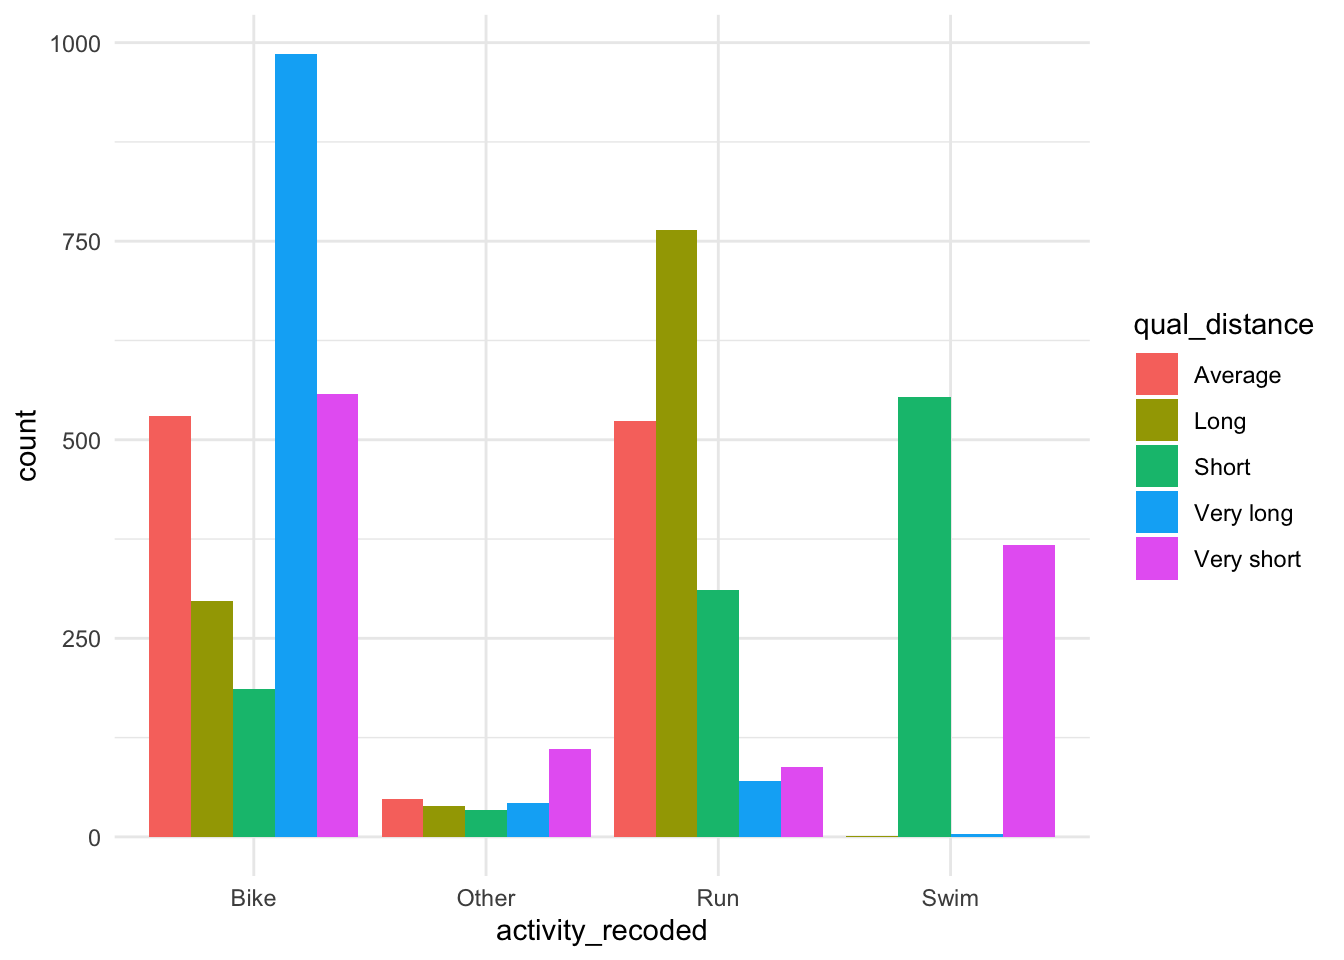
\includegraphics{DataExploration_files/figure-latex/unnamed-chunk-53-2.pdf}

\begin{Shaded}
\begin{Highlighting}[]
\KeywordTok{ggplot}\NormalTok{(dat,}\KeywordTok{aes}\NormalTok{(activity_recoded,}\DataTypeTok{fill=}\NormalTok{qual_distance)) }\OperatorTok{+}\StringTok{ }
\StringTok{  }\KeywordTok{geom_bar}\NormalTok{(}\DataTypeTok{position =} \StringTok{"fill"}\NormalTok{) }\OperatorTok{+}\StringTok{ }
\StringTok{  }\KeywordTok{scale_y_continuous}\NormalTok{(}\DataTypeTok{labels =}\NormalTok{ scales}\OperatorTok{::}\NormalTok{percent) }\OperatorTok{+}\StringTok{ }\KeywordTok{theme_minimal}\NormalTok{()}
\end{Highlighting}
\end{Shaded}

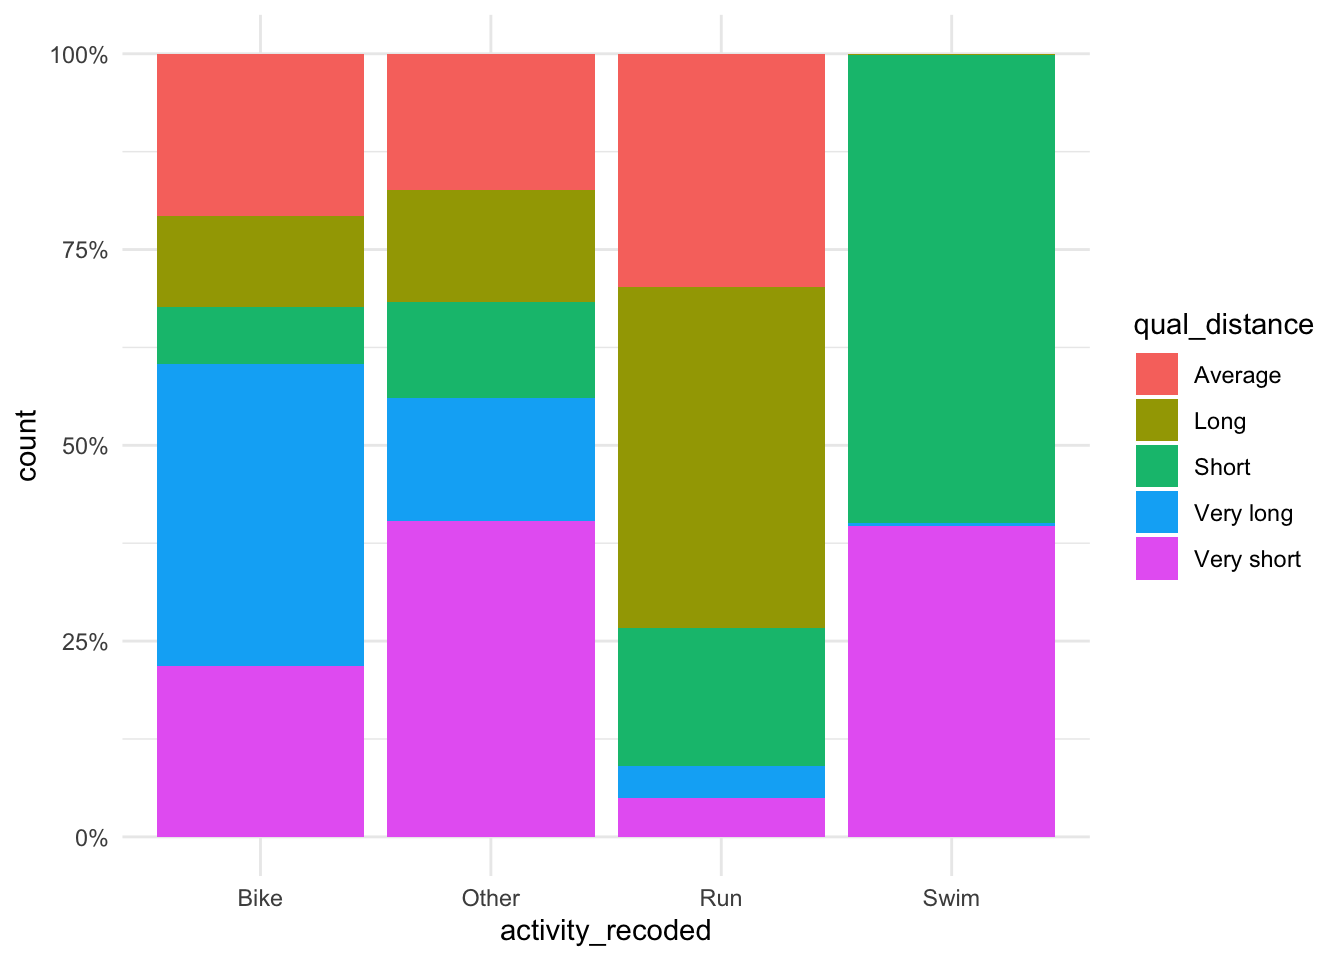
\includegraphics{DataExploration_files/figure-latex/unnamed-chunk-53-3.pdf}

You get really different insights depending on the representation you chose !

\hypertarget{contingency-tables-1}{%
\subsubsection{Contingency tables}\label{contingency-tables-1}}

\begin{Shaded}
\begin{Highlighting}[]
\KeywordTok{table}\NormalTok{(dat}\OperatorTok{$}\NormalTok{activity_recoded,dat}\OperatorTok{$}\NormalTok{qual_distance) }
\end{Highlighting}
\end{Shaded}

\begin{verbatim}
##        
##         Average Long Short Very long Very short
##   Bike      530  297   186       986        558
##   Other      48   39    34        43        111
##   Run       523  764   311        70         88
##   Swim        0    1   554         3        368
\end{verbatim}

\begin{Shaded}
\begin{Highlighting}[]
\KeywordTok{table}\NormalTok{(dat}\OperatorTok{$}\NormalTok{activity_recoded,dat}\OperatorTok{$}\NormalTok{qual_distance) }\OperatorTok\StringTok{   }
\StringTok{  }\KeywordTok{prop.table}\NormalTok{()}\OperatorTok{*}\DecValTok{100}
\end{Highlighting}
\end{Shaded}

\begin{verbatim}
##        
##             Average        Long       Short   Very long  Very short
##   Bike   9.61189699  5.38628945  3.37323177 17.88175553 10.11969532
##   Other  0.87051143  0.70729053  0.61661226  0.77983315  2.01305767
##   Run    9.48494741 13.85564019  5.64018861  1.26949583  1.59593761
##   Swim   0.00000000  0.01813565 10.04715270  0.05440696  6.67392093
\end{verbatim}

\begin{Shaded}
\begin{Highlighting}[]
\KeywordTok{table}\NormalTok{(dat}\OperatorTok{$}\NormalTok{activity_recoded,dat}\OperatorTok{$}\NormalTok{qual_distance) }\OperatorTok\StringTok{   }
\StringTok{  }\KeywordTok{prop.table}\NormalTok{(}\DataTypeTok{margin =} \DecValTok{1}\NormalTok{)}\OperatorTok{*}\DecValTok{100}
\end{Highlighting}
\end{Shaded}

\begin{verbatim}
##        
##            Average       Long      Short  Very long Very short
##   Bike  20.7274149 11.6151740  7.2741494 38.5608135 21.8224482
##   Other 17.4545455 14.1818182 12.3636364 15.6363636 40.3636364
##   Run   29.7835991 43.5079727 17.7107062  3.9863326  5.0113895
##   Swim   0.0000000  0.1079914 59.8272138  0.3239741 39.7408207
\end{verbatim}

\begin{Shaded}
\begin{Highlighting}[]
\KeywordTok{table}\NormalTok{(dat}\OperatorTok{$}\NormalTok{activity_recoded,dat}\OperatorTok{$}\NormalTok{qual_distance) }\OperatorTok\StringTok{   }
\StringTok{  }\KeywordTok{prop.table}\NormalTok{(}\DataTypeTok{margin =} \DecValTok{2}\NormalTok{)}\OperatorTok{*}\DecValTok{100}
\end{Highlighting}
\end{Shaded}

\begin{verbatim}
##        
##             Average        Long       Short   Very long  Very short
##   Bike  48.13805631 26.97547684 17.14285714 89.47368421 49.60000000
##   Other  4.35967302  3.54223433  3.13364055  3.90199637  9.86666667
##   Run   47.50227066 69.39146231 28.66359447  6.35208711  7.82222222
##   Swim   0.00000000  0.09082652 51.05990783  0.27223230 32.71111111
\end{verbatim}

\hypertarget{quantifying-relationships-chi2-cramers-v}{%
\subsubsection{\texorpdfstring{Quantifying relationships : \(\chi^2\), Cramer's V}{Quantifying relationships : \textbackslash chi\^{}2, Cramer's V}}\label{quantifying-relationships-chi2-cramers-v}}

The Chi-square (\(\chi^2\)) statistics is used to measure the distance between the actual distribution of cases among categories of both variables and the distribution if the variables were independant. The higher the \texttt{X-squared}, the higher the divergence with independance, meaning that the variables are likely \emph{linked} (correlation does not apply to categorical variables). The \texttt{p-value} indicates whether this relationship is \textbf{statistically significant} or not. We will see this in more details in the last chapter (Inference).

More info and detailed way to compute the value : \href{https://www.statisticshowto.com/probability-and-statistics/chi-square/}{this website}

\hypertarget{extreme-examples}{%
\subsubsection{Extreme examples :}\label{extreme-examples}}

Let's assume we want to assess the relationship between gender and churn. Further assumption, we have 100 customers, 50 males, 50 females on the one hand, 50 churners, 50 non churners on the other hand.

\begin{itemize}
\tightlist
\item
  If the variables are independent, the cross table would look that way :
\end{itemize}

\begin{verbatim}
## 
## 	Pearson's Chi-squared test
## 
## data:  .
## X-squared = 0, df = 12, p-value = 1
\end{verbatim}

\begin{itemize}
\tightlist
\item
  In the opposite situation (full dependency), the contingency table would look like that :
\end{itemize}

\begin{verbatim}
##       Short Very long Long Average
## Swim     25         0    0       0
## Bike      0        25    0       0
## Run       0         0   25       0
## Other     0         0    0      25
\end{verbatim}

The \(\chi^2\) statistic measures the ``distance'' between reality and the first case (independence)

\textbf{Note :} if some cells of the contingency table have less than 5 cases, the statistic is not reliable (you'll get a message in this case)

The chi-square suffers 2 main drawbacks : its value depends on the number of observations and the total number of categories \(\Rightarrow\) one cannot compare the \(\chi^2\) values for 2 different tables that have different numbers of underlying observations and number of categories.
To deal with that, you can use Cramer's V, which is a (kind of) \emph{normalized} \(\chi^2\). You can use the function built in the \texttt{lsr} package. Cramer's V \(\in [0,1]\) and the higher it is, the more intense the link between both variables.

\begin{Shaded}
\begin{Highlighting}[]
\CommentTok{# install.packages("lsr") # If not installed}
\KeywordTok{table}\NormalTok{(dat}\OperatorTok{$}\NormalTok{activity_recoded,dat}\OperatorTok{$}\NormalTok{qual_distance) }\OperatorTok\StringTok{ }
\StringTok{  }\NormalTok{lsr}\OperatorTok{::}\KeywordTok{cramersV}\NormalTok{()}
\end{Highlighting}
\end{Shaded}

\begin{verbatim}
## [1] 0.4454809
\end{verbatim}

Let's check with our 2 extreme examples :

\begin{Shaded}
\begin{Highlighting}[]
\NormalTok{lsr}\OperatorTok{::}\KeywordTok{cramersV}\NormalTok{(ex_dep[,}\OperatorTok{-}\DecValTok{5}\NormalTok{])}
\end{Highlighting}
\end{Shaded}

\begin{verbatim}
## [1] 1
\end{verbatim}

\begin{Shaded}
\begin{Highlighting}[]
\NormalTok{lsr}\OperatorTok{::}\KeywordTok{cramersV}\NormalTok{(ex_indep)}
\end{Highlighting}
\end{Shaded}

\begin{verbatim}
## [1] 0
\end{verbatim}

In practice, it is very rare to get high values ; a rule of thumb is that a value around 0.2-0.3 is already ``decent''. The \(\chi^2\) p-value (if under 0.05) shows that there is a relationship ; Cramer's V allows to compare between two tables.

\hypertarget{continuous-1-categorical-variable}{%
\subsection{1 continuous, 1 categorical variable}\label{continuous-1-categorical-variable}}

In this part, we see how to deal with 2 variables that have different types. The goal remains the same : getting insights about the relationship between those 2 variables and quantify the strength of the link.
We will try to assess if there is a connection between the distance and the discipline.

\hypertarget{boxplots-violin-plots}{%
\subsubsection{Boxplots, violin plots}\label{boxplots-violin-plots}}

Boxplots are a simple, effective and compact representation of a variable's distribution. It relies on quantiles.
Vilin plots allows to see the ful distribution of both variables

\begin{Shaded}
\begin{Highlighting}[]
\CommentTok{# Compute bounds of the boxplot}
\CommentTok{# bounds <- group_by(dat,activity_recoded) %>% }
\CommentTok{#   summarise(q1=quantile(distance,.25,na.rm = T),}
\CommentTok{#             q2=quantile(distance,.50,na.rm = T),}
\CommentTok{#             q3=quantile(distance,.75,na.rm = T),}
\CommentTok{#             lower_bound=q1-1.5*IQR(distance,na.rm = T),}
\CommentTok{#             upper_bound=q3+1.5*IQR(distance,na.rm = T)) %>% }
\CommentTok{#   pivot_longer(-activity_recoded)}
\KeywordTok{ggplot}\NormalTok{(dat,}\KeywordTok{aes}\NormalTok{(activity_recoded,distance}\OperatorTok{/}\FloatTok{1E5}\NormalTok{)) }\OperatorTok{+}\StringTok{ }\KeywordTok{geom_boxplot}\NormalTok{() }\OperatorTok{+}\StringTok{ }\KeywordTok{theme_minimal}\NormalTok{()}
\end{Highlighting}
\end{Shaded}

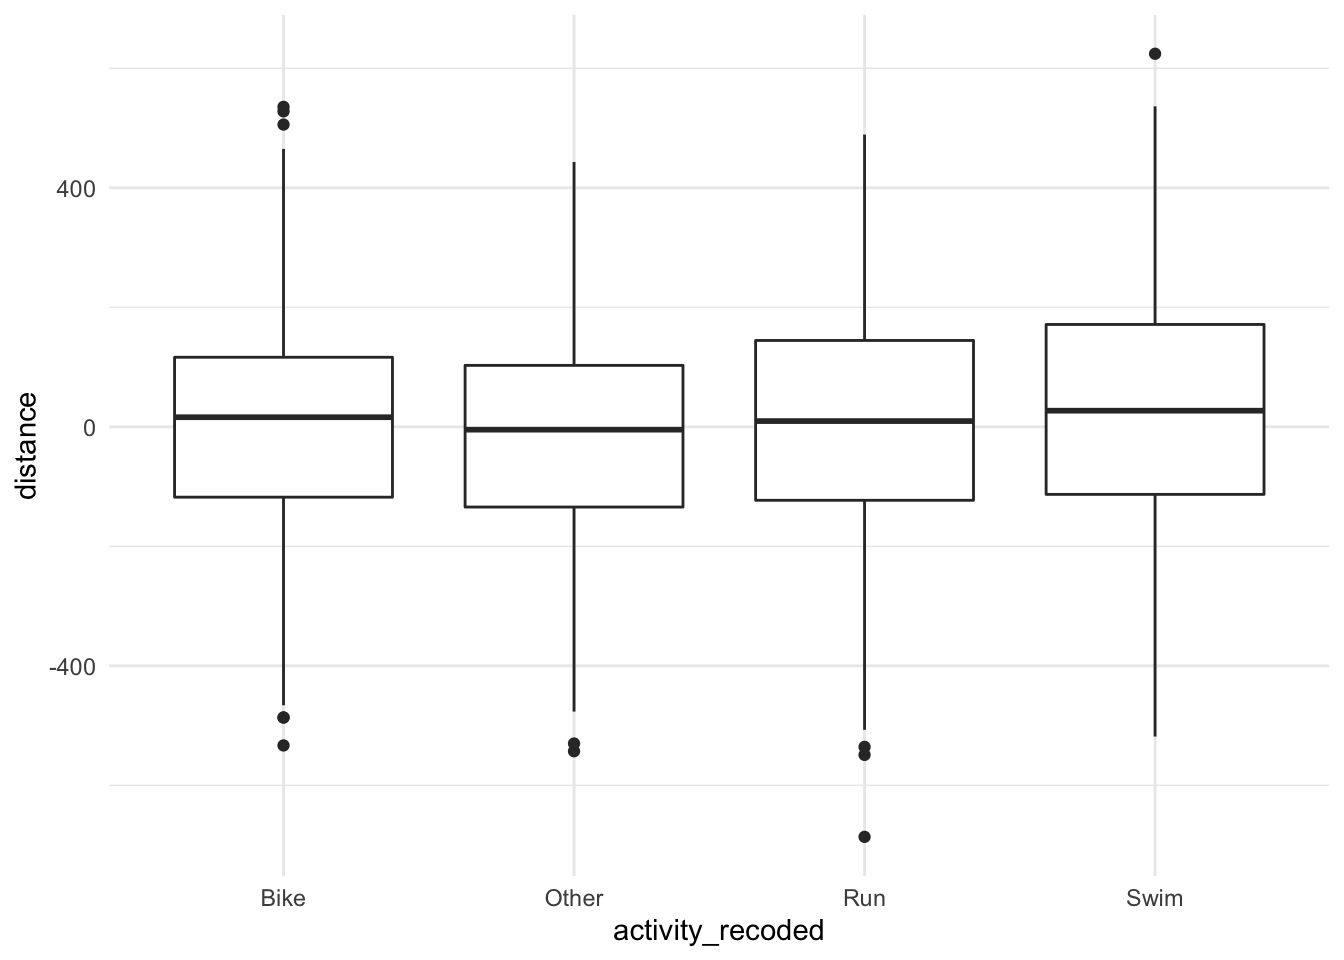
\includegraphics{DataExploration_files/figure-latex/unnamed-chunk-59-1.pdf}

\begin{Shaded}
\begin{Highlighting}[]
  \CommentTok{# geom_point(data = bounds,aes(activity_recoded,value,color=name))}
\KeywordTok{ggplot}\NormalTok{(dat,}\KeywordTok{aes}\NormalTok{(activity_recoded,distance}\OperatorTok{/}\FloatTok{1E5}\NormalTok{)) }\OperatorTok{+}\StringTok{ }\KeywordTok{geom_violin}\NormalTok{()}\OperatorTok{+}\StringTok{ }\KeywordTok{theme_minimal}\NormalTok{() }\OperatorTok{+}\StringTok{ }\KeywordTok{scale_y_log10}\NormalTok{(}\DataTypeTok{label=}\NormalTok{scales}\OperatorTok{::}\NormalTok{comma)}
\end{Highlighting}
\end{Shaded}

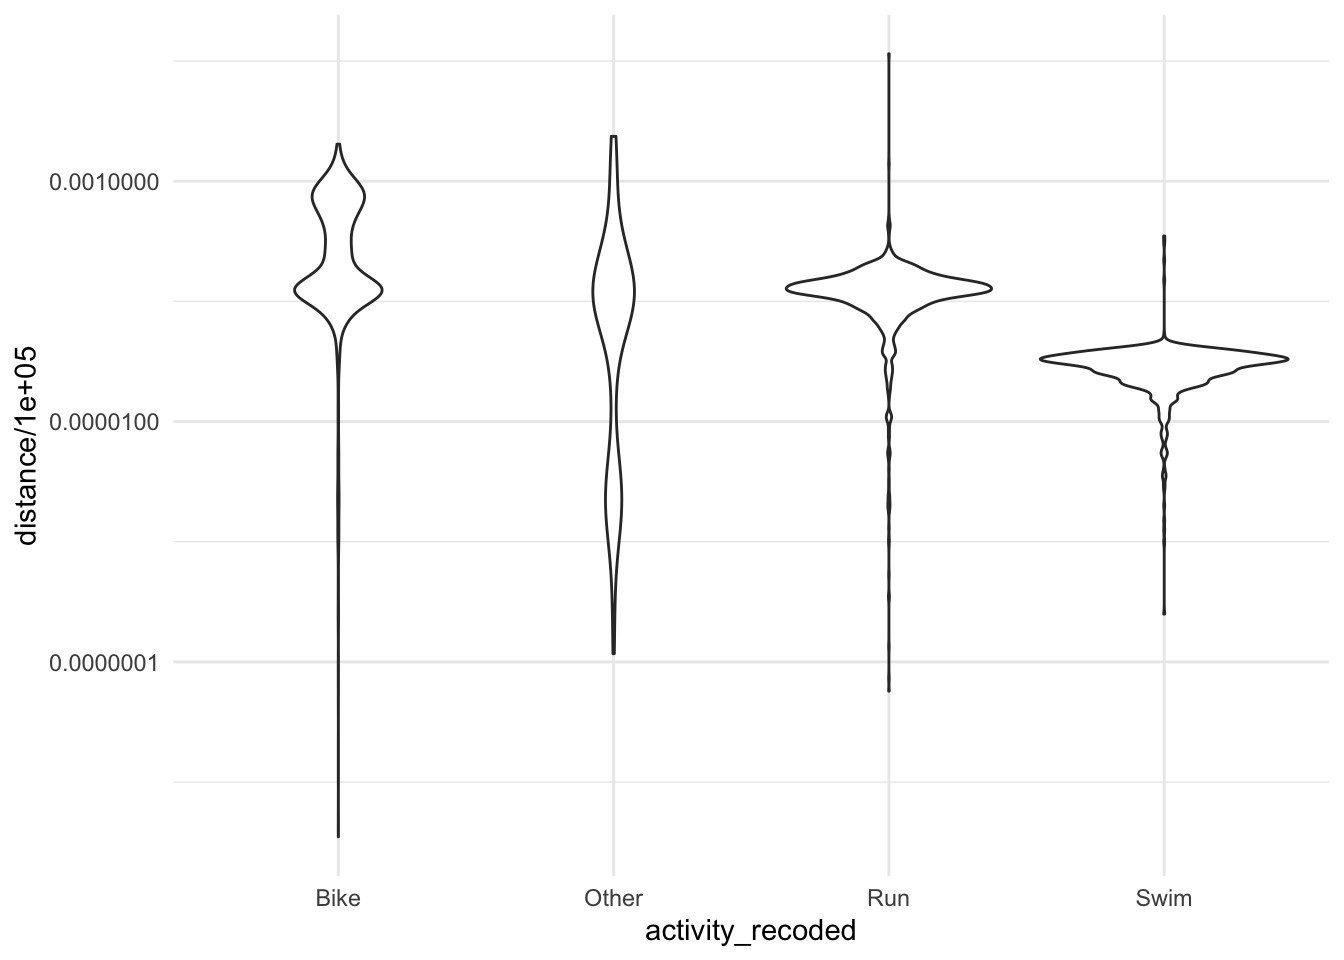
\includegraphics{DataExploration_files/figure-latex/unnamed-chunk-59-2.pdf}

It looks like bike activities are longer than the others ! Big surprise !

\hypertarget{quantifying-relationship-intensity-eta2}{%
\subsubsection{\texorpdfstring{Quantifying relationship intensity : \(\eta^2\)}{Quantifying relationship intensity : \textbackslash eta\^{}2}}\label{quantifying-relationship-intensity-eta2}}

The graphics indicate that there is a relationship between activity type and distance (if not, boxplots would have the same shape for all groups). We can assess the strength of the connection with the \(\eta^2\) statistics.

Using the decomposition of the variance formula \(SS_{total} = SS_{between} + SS_{within}\), \(\eta^2\) is defined as \(\eta^2 = \dfrac{SS_{between}}{SS_{total}} \in [0,1]\)

\hypertarget{extreme-examples-1}{%
\subsubsection{Extreme examples :}\label{extreme-examples-1}}

\begin{itemize}
\tightlist
\item
  If the variables are independent, the boxplots should look like this (almost no difference in the distributions) :
\end{itemize}

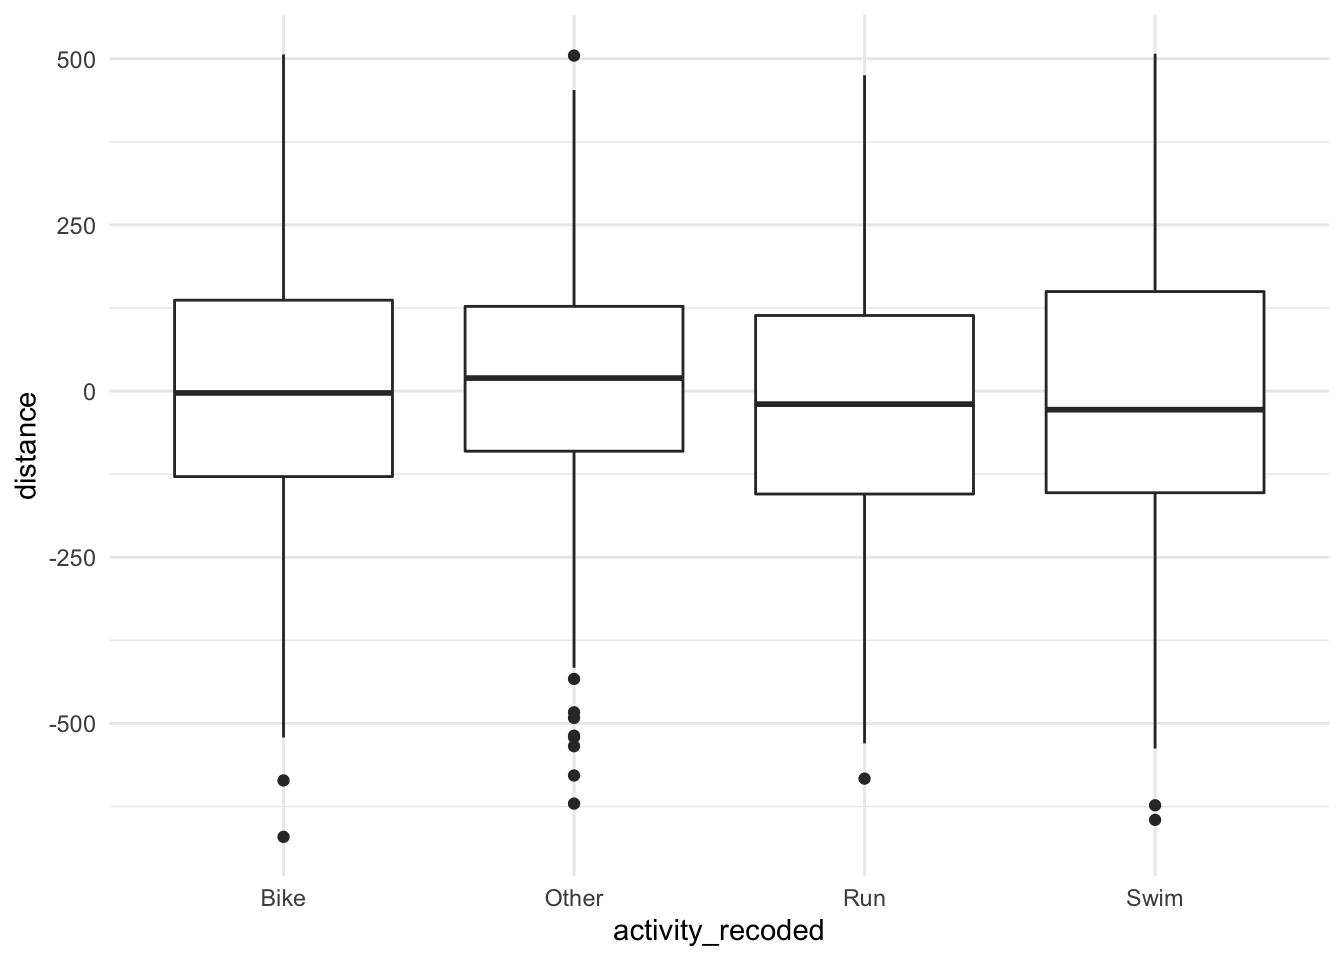
\includegraphics{DataExploration_files/figure-latex/unnamed-chunk-60-1.pdf}

\begin{itemize}
\tightlist
\item
  If they are fully ``correlated'', the activity variable would explain all variance in the data set :
\end{itemize}

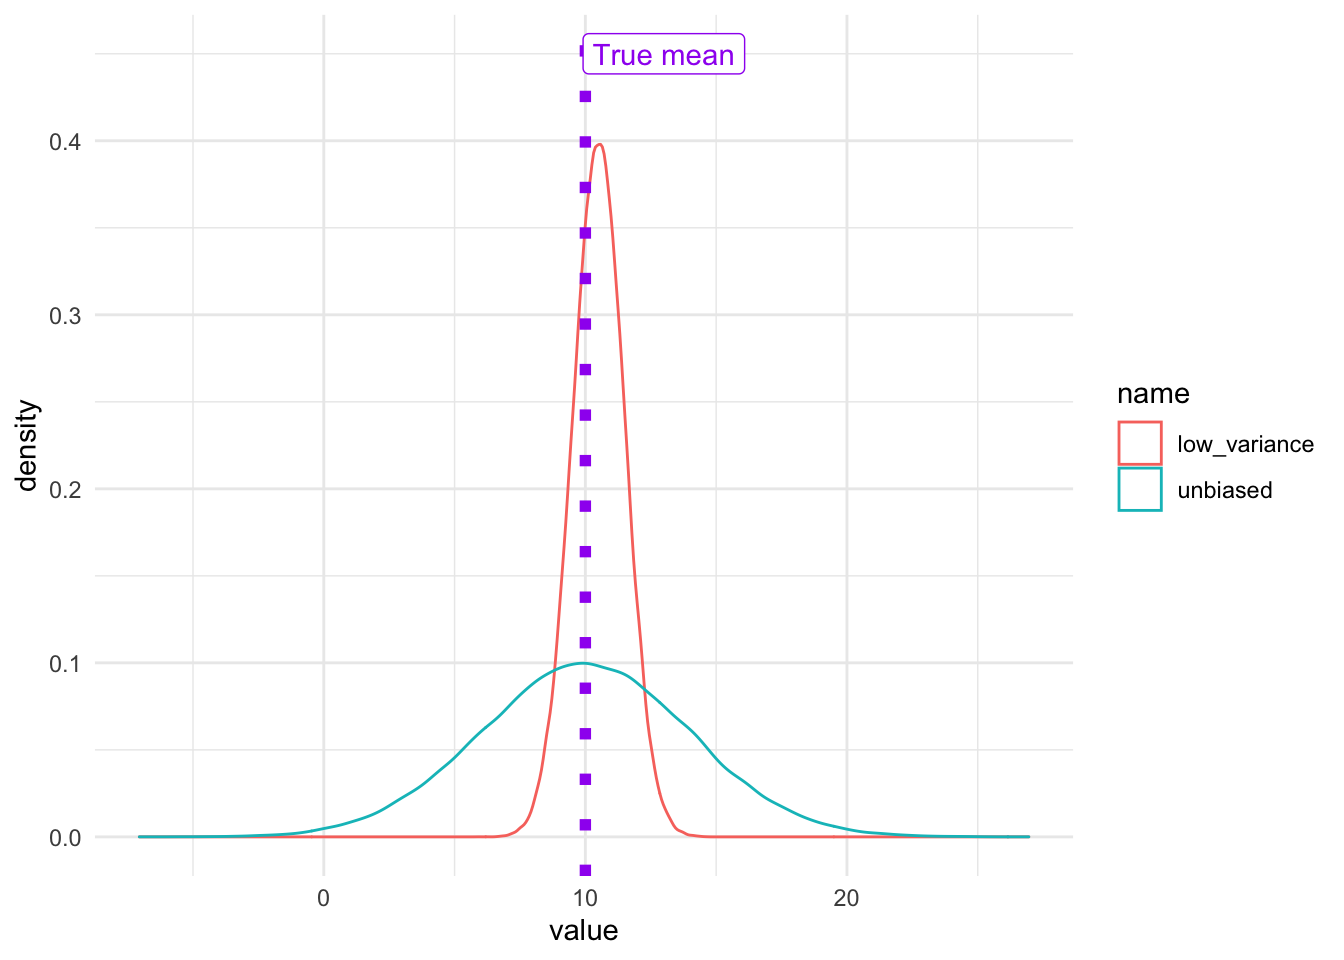
\includegraphics{DataExploration_files/figure-latex/unnamed-chunk-61-1.pdf}

In this case, we see that all the variance lies between the subgroups : there is no dispersion within the groups.

\textbf{Note :} In practice, the previous situation will of course never happen, and a categorical variable can't carry by itself a lot of variance (since the number of possible values are de facto limited).

This is also the \(R^2\) of the 1-factor ANOVA regression of distance explained by activty type,

\begin{Shaded}
\begin{Highlighting}[]
\NormalTok{anova <-}\StringTok{ }\KeywordTok{aov}\NormalTok{(distance}\OperatorTok{~}\NormalTok{activity_recoded,}\DataTypeTok{data=}\NormalTok{dat) }
\CommentTok{# Variance decomposition}
\KeywordTok{summary}\NormalTok{(anova)}
\end{Highlighting}
\end{Shaded}

\begin{verbatim}
##                    Df  Sum Sq Mean Sq F value Pr(>F)    
## activity_recoded    3  610577  203526   230.6 <2e-16 ***
## Residuals        5503 4857888     883                   
## ---
## Signif. codes:  0 '***' 0.001 '**' 0.01 '*' 0.05 '.' 0.1 ' ' 1
## 7 observations deleted due to missingness
\end{verbatim}

\begin{Shaded}
\begin{Highlighting}[]
\KeywordTok{print}\NormalTok{(}\StringTok{"eta squared"}\NormalTok{)}
\end{Highlighting}
\end{Shaded}

\begin{verbatim}
## [1] "eta squared"
\end{verbatim}

\begin{Shaded}
\begin{Highlighting}[]
\NormalTok{lsr}\OperatorTok{::}\KeywordTok{etaSquared}\NormalTok{(anova)}
\end{Highlighting}
\end{Shaded}

\begin{verbatim}
##                     eta.sq eta.sq.part
## activity_recoded 0.1116542   0.1116542
\end{verbatim}

\begin{Shaded}
\begin{Highlighting}[]
\CommentTok{# Alternatively}
\KeywordTok{lm}\NormalTok{(distance}\OperatorTok{~}\NormalTok{activity_recoded,}\DataTypeTok{data=}\NormalTok{dat) }\OperatorTok\StringTok{ }\KeywordTok{summary}\NormalTok{()}
\end{Highlighting}
\end{Shaded}

\begin{verbatim}
## 
## Call:
## lm(formula = distance ~ activity_recoded, data = dat)
## 
## Residuals:
##     Min      1Q  Median      3Q     Max 
##  -29.98  -17.47   -1.23    1.37 1136.08 
## 
## Coefficients:
##                       Estimate Std. Error t value Pr(>|t|)    
## (Intercept)            29.9816     0.5877  51.017  < 2e-16 ***
## activity_recodedOther -11.9153     1.8950  -6.288 3.47e-10 ***
## activity_recodedRun   -17.0613     0.9214 -18.517  < 2e-16 ***
## activity_recodedSwim  -27.0224     1.1396 -23.712  < 2e-16 ***
## ---
## Signif. codes:  0 '***' 0.001 '**' 0.01 '*' 0.05 '.' 0.1 ' ' 1
## 
## Residual standard error: 29.71 on 5503 degrees of freedom
##   (7 observations deleted due to missingness)
## Multiple R-squared:  0.1117,	Adjusted R-squared:  0.1112 
## F-statistic: 230.6 on 3 and 5503 DF,  p-value: < 2.2e-16
\end{verbatim}

In this case, 11.2\% of the age variance is explained by the difference in activity types ; it is very high.

\hypertarget{exercises-1}{%
\subsection{Exercises}\label{exercises-1}}

\begin{itemize}
\tightlist
\item
  Explore the distribution of the average speed. What can you say about it ?
\item
  Explore the correlation between average speed and average power
\item
  For all the the categorical variables, get the frequent category (with table AND dplyr/tidyr)
\end{itemize}

\textbf{Very important :} For the next parts, we will remove the extreme observation that is clearly an error

\begin{Shaded}
\begin{Highlighting}[]
\NormalTok{dat_clean <-}\StringTok{ }\KeywordTok{filter}\NormalTok{(dat,}\OperatorTok{!}\NormalTok{(activityId }\OperatorTok\StringTok{ }\KeywordTok{c}\NormalTok{(}\DecValTok{407226313}\NormalTok{,}\DecValTok{2321338}\NormalTok{)) }\OperatorTok{&}\StringTok{ }\KeywordTok{year}\NormalTok{(date)}\OperatorTok{>=}\DecValTok{2012}\NormalTok{)}
\end{Highlighting}
\end{Shaded}

\hypertarget{stat_inf}{%
\section{Statistical inference}\label{stat_inf}}

\hypertarget{the-statistical-model}{%
\subsection{The statistical model}\label{the-statistical-model}}

We want to measure a characteristic in the \emph{general population}, let's say the average distance of all potential activites, and let's denote it by D.

The fundamental assumption of the statistical model is that there is an underlying \emph{data-genereting process}, which means that D is distributed with a certain probability distribution. The goal of the statistician is to find which distribution it is, and estimate its parameters.

The big problem is that it is impossible to observe D on the whole population, and any dataset is only a \textbf{sample of the general population} (which does not really exists). The question is then : how can we estimate the parameters of the \emph{true} distribution ?

\(\Rightarrow\) There is a difference between the \textbf{sample mean} and the \textbf{population mean} (noted \(\mu\)).
As a matter of fact the sample mean is an estimator of the population mean. The value of an estimator (often noted \(\hat{\theta}\)) is a random variable (it depends on the sample), meaning this is not a single deterministic value, but has a probability distribution. Therefore it has an \textbf{expectation} and a \textbf{variance}
An estimator is said to be \emph{biased} if \(\mathbb{E}(\hat{\theta}) \neq \mu\) ; it is said to be \emph{efficient} if its variance is minimal.

One fundamental hypothesis of the model is that all observations are independent and identically distributed (\emph{iid}). This is typically not the case for \emph{time series}, but this hypothesis is, in general, reasonable.

\hypertarget{two-fundamental-theorems}{%
\subsection{Two fundamental theorems}\label{two-fundamental-theorems}}

Eventough we cannot observe the true parameter(s), and that the sample mean is an estimator (hence a random variable), 2 theorems save the game :

\hypertarget{the-law-of-large-numbers}{%
\subsubsection{The law of large numbers}\label{the-law-of-large-numbers}}

\[\bar{D} = \dfrac{1}{n} \sum_{i=1}^n D_i \xrightarrow[n \to +\infty]{a.s.} \mu\]

In other words, when the sample size n is big enough, the sample mean converges to the population mean \(\rightarrow\) We can estimate this parameter with a simple mean without \textbf{bias}.

\hypertarget{the-central-limit-theorem-clt}{%
\subsubsection{The central limit theorem (CLT)}\label{the-central-limit-theorem-clt}}

Probably the most important theorem in statistics, valid whatever the true distribution is

\[\sqrt{n} \cdot \bar{D} \xrightarrow[n \to +\infty]{p}  \mathcal{N} (\mu,\sigma^2)\]

Meaning that the sample mean converges in probability to a normal distribution with population parameters at ``speed'' \(\sqrt{n}\). This is equivalent to :

\[ \bar{D} - \mu \xrightarrow[n \to +\infty]{p}  \mathcal{N} (0,\frac{\sigma^2}{n})\]

Meaning that :

\begin{itemize}
\tightlist
\item
  I can quantify ``how far'' my sample mean is from the true value
\item
  The larger the sample size, the smaller the average deviation to the true value \(\rightarrow\) the variance of my estimator reduces when the sample size increases.
\end{itemize}

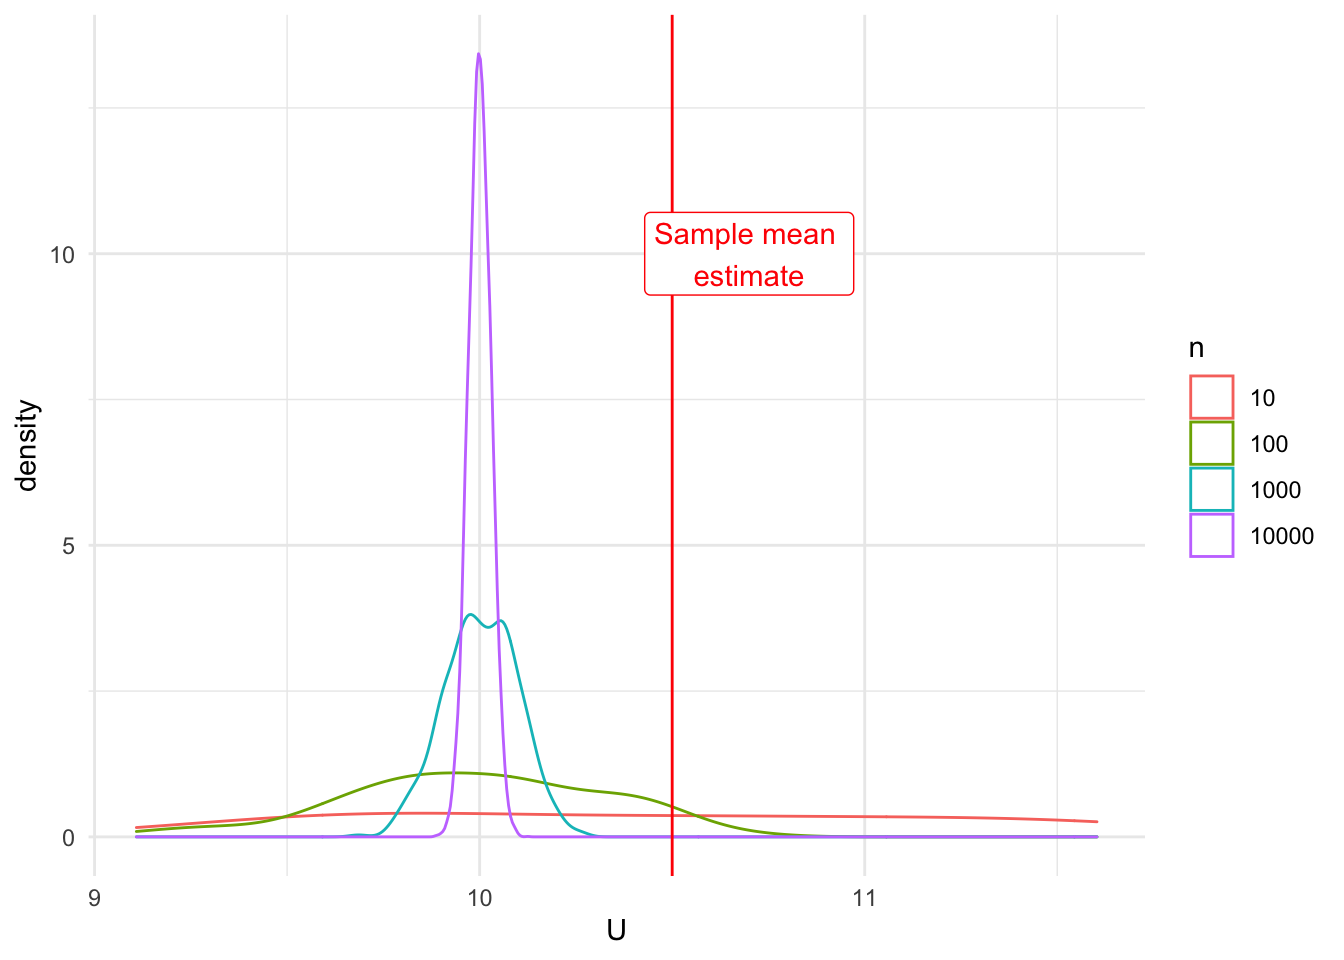
\includegraphics{DataExploration_files/figure-latex/unnamed-chunk-64-1.pdf}

Take away :

\begin{itemize}
\tightlist
\item
  The \textbf{sample mean} is an \textbf{estimator} of the true value of an underlying ``true'' mean. The estimator's value depends on the sample I have
\item
  This estimator (any estimator) has a \textbf{variance} that I could measure if I had several samples to compute several sample means
\item
  Probality theory gives us tools to estimate the \textbf{bias} and \textbf{the variance} of an estimator
\item
  \textbf{Bias-variance trade-off} :\(\mathbb{E}((D-\bar{D})^2)=\mathbb{E}^2(D-\bar{D}) + \mathbb{V}(\bar{D})\), in other words : \(MSE_{\bar{D}} = bias^2 + \mathbb{V}(\bar{D})\) \(\rightarrow\) see you during ML course ;-)
\end{itemize}

Illustration of the biais-variance trade-off.

Let's assume the \textbf{true} average of the usage is 10, what do you prefer over the following scenarios ? Let's simulate two distributions (let's say it is the distribution of 2 different estimators) :

\begin{itemize}
\tightlist
\item
  One with mean 10 and variance 4 \(\rightarrow\) unbiased
\item
  The second with mean 10.5 and variance 1 \(\rightarrow\) biased but with low variance
\end{itemize}

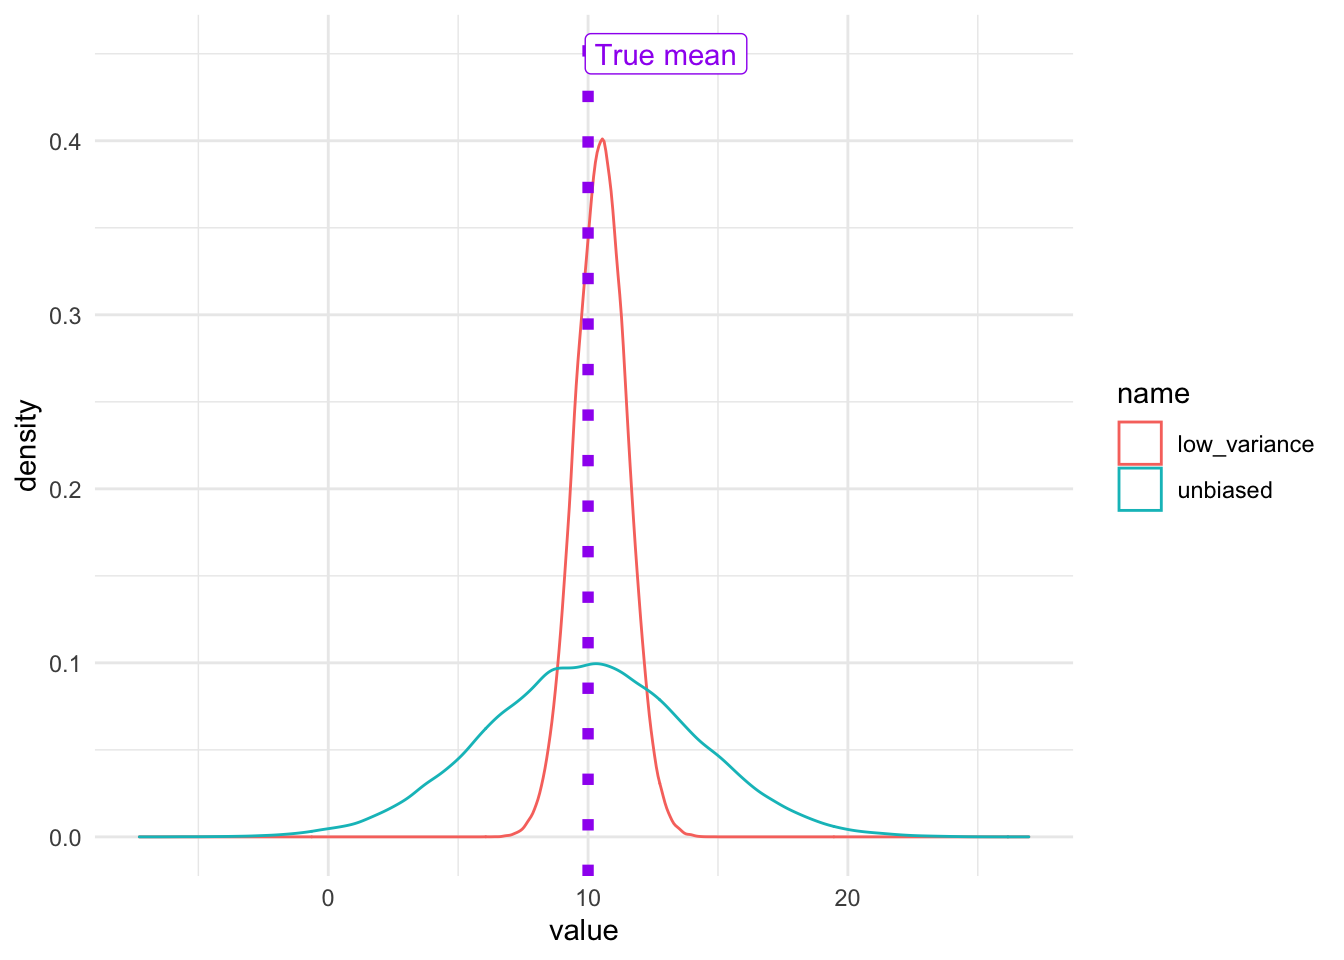
\includegraphics{DataExploration_files/figure-latex/unnamed-chunk-65-1.pdf}

In the first case, the estimator is unbiased, but with a higher variance than the second : if we go for it, we take the chance to have an estimate (depending on our sample) of eg 15 or 5, which is almost unlikely to happen with the second estimator, although this second is not centered on the true value.
It is up to you to decide, but you generally can't have both an unbiased and very precise estimator\ldots{}

\hypertarget{statistical-tests}{%
\subsection{Statistical tests}\label{statistical-tests}}

\hypertarget{introductory-example}{%
\subsubsection{Introductory example}\label{introductory-example}}

Knowing the theoretical probability distribution of our estimator, we can assess the likelihood of an hypothesis. For the example, let's make the hypothesis (\(\mathcal{H_0}\)) that the true mean is 10 and standard deviation is \(2\sqrt{n}\). If this hypothesis is true, thanks to the CTL, the distribution of \(\bar{D}\) would be the following :

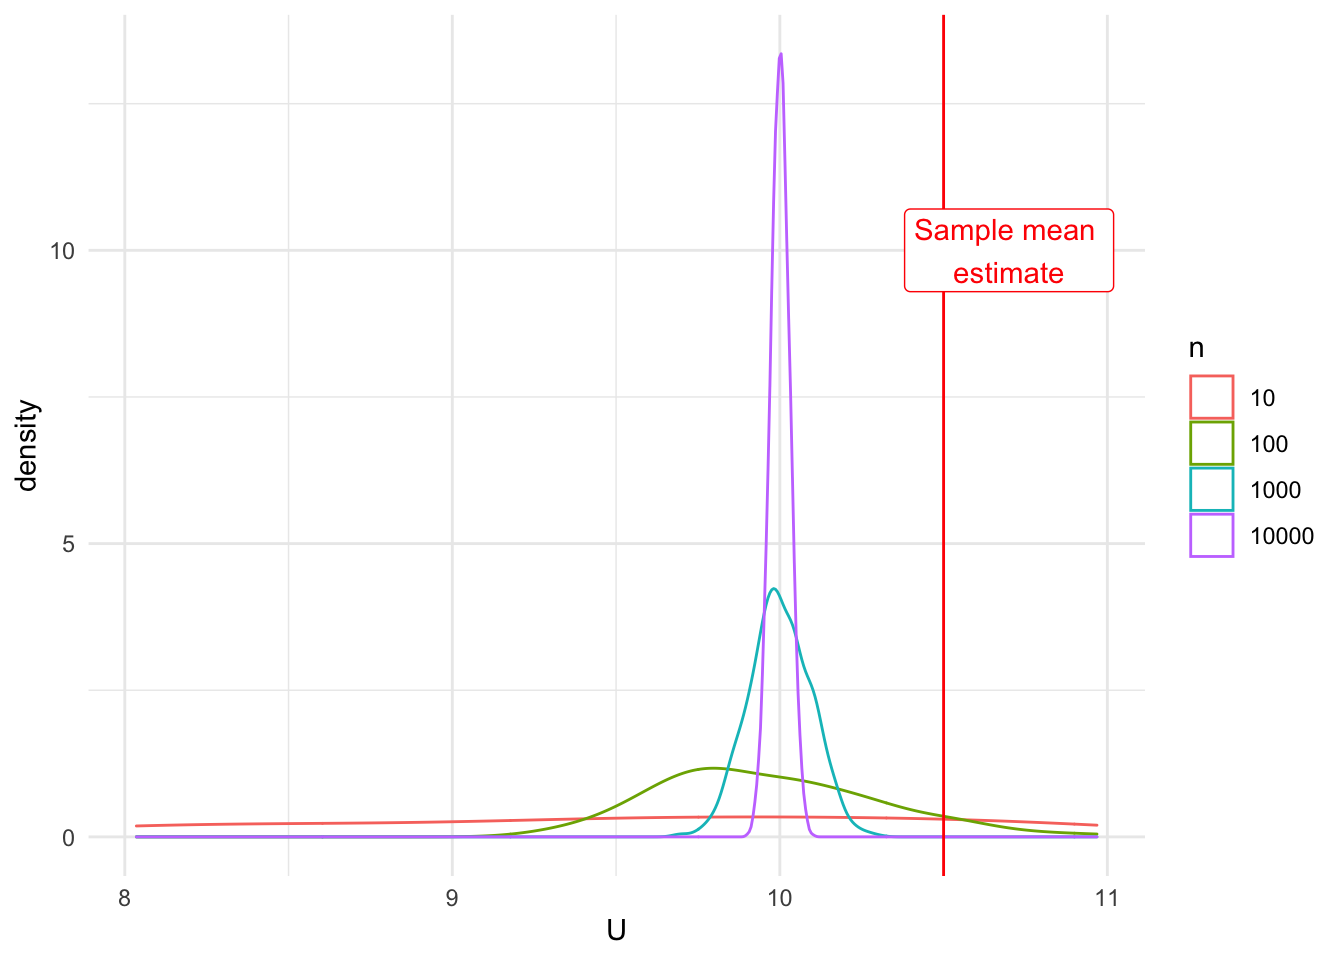
\includegraphics{DataExploration_files/figure-latex/unnamed-chunk-66-1.pdf}

Now, I can compute my sample mean and check its value against the hypothetical distribution :

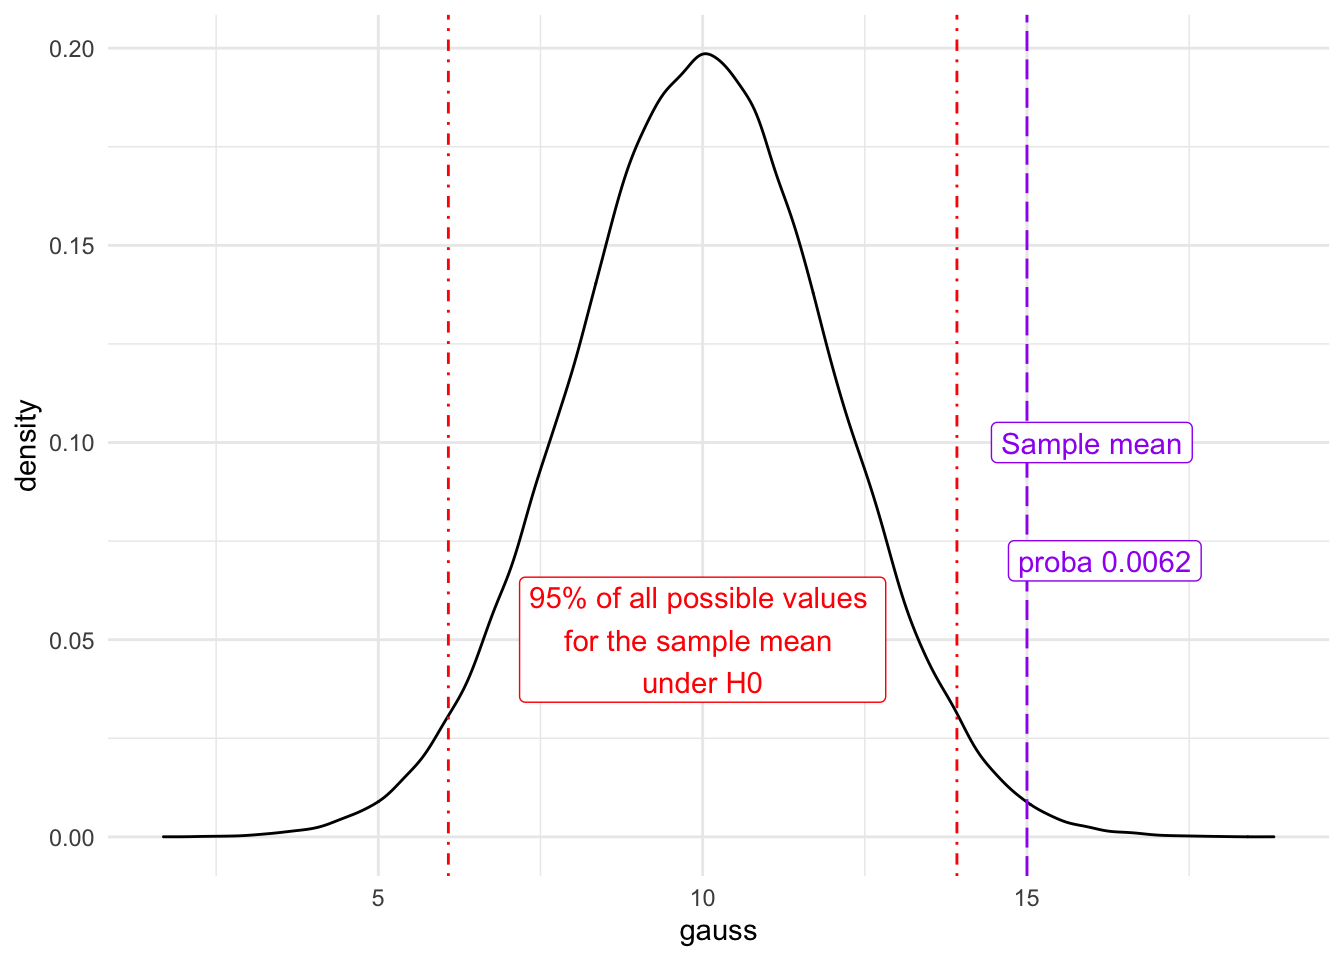
\includegraphics{DataExploration_files/figure-latex/unnamed-chunk-67-1.pdf}

Obviously my actual value doesn't fit with my hypothesis : the probability of getting such a sample mean under \(\mathcal{H_O}\) is very small \(\rightarrow\) my hypothesis is very unlikely to be valid \(\rightarrow\) the true mean is probably not 10.

\hypertarget{student-test}{%
\subsubsection{Student test}\label{student-test}}

A test is defined by its \emph{null hypothesis} \(\mathcal{H_0}\), the contrapositive (alternative) being \(\mathcal{H_1}\). The general procedure is to set \(\mathcal{H_0}\) such that we can build a \emph{test statistic} of which we can derive the distribution.

In general, statisticians chose a null hypothesis such that they can build a statistic for which they know the distribution \(\rightarrow\) they can compute the probability of a specific value to occur.

For the example, we'll focus on the \textbf{Student test}. The test is meant to check whether the true value of the mean is equal to a specific value. Example, I want to test whether the average distance for all activities is 20km/h. Our test is the following :

\begin{itemize}
\tightlist
\item
  \(\mathcal{H_0}\) : The average distance of activities is 20
\item
  \(\mathcal{H_1}\) : The average distance of activities is not 20
\end{itemize}

The next important parameter of a test if \(\alpha\), the risk level, meaning the probability we are willing to take to be wrong while accepting \(\mathcal{H_0}\). 5\% is a value that is often chosen.

Thanks to the CLT, we can build the following test statistic :

\[T = \sqrt{n} \dfrac{\bar{D}-20}{\sigma} \hookrightarrow \mathcal{N}(0,1)\]

Problem : we don't know the value of the true standard deviation. The final test statistic is distributed with a Student distribution :

\[T = \sqrt{n} \dfrac{\bar{D}-20}{\hat{s}} \hookrightarrow \mathcal{St}_{n-1}\]

where \(\hat{s}^2 = \dfrac{1}{n-1}\sum_{i=1}^n (D-\bar{D})^2\) is the unbiased estimator of the variance.

\hypertarget{implementation-in-r}{%
\paragraph{Implementation in R :}\label{implementation-in-r}}

\begin{Shaded}
\begin{Highlighting}[]
\KeywordTok{t.test}\NormalTok{(dat}\OperatorTok{$}\NormalTok{distance,}\DataTypeTok{mu=}\DecValTok{20}\NormalTok{)}
\end{Highlighting}
\end{Shaded}

\begin{verbatim}
## 
## 	One Sample t-test
## 
## data:  dat$distance
## t = -1.3698, df = 5506, p-value = 0.1708
## alternative hypothesis: true mean is not equal to 20
## 95 percent confidence interval:
##  18.58573 20.25079
## sample estimates:
## mean of x 
##  19.41826
\end{verbatim}

\hypertarget{interpretation}{%
\paragraph{Interpretation :}\label{interpretation}}

If you have one thing to remember : \textbf{the p-value is the probability to be wrong while rejecting \(\mathcal{H_0}\)}.
In our case, this probability is very small, meaning that we should not consider that the average distance of all activities is 20km/h.

In short : all you have to know is what the null hypothesis is, and make your decision depending on the p-value. In general, we reject the null is p-value \textless{} 5\% (the risk level), but you can decide to be more demanding and chose a lower threshold if you don't want to make a mistake.

\emph{Note : } If you want to dig deeper, you can test whether the mean is strictly greater than a specific value using the parameter \texttt{alternative} of the \texttt{t-test} function.

\hypertarget{student-test-to-compare-group-means}{%
\subsubsection{Student test to compare group means}\label{student-test-to-compare-group-means}}

You can also use the Student test to check whether the means of two sub-populations are equal or not. In this case, the tests checks whether the difference in means differs significantly from 0. We'll check in this example if average distance differs between rides and other activities.
For that we have to extract on the one hand the bike activities' distance and the other activites' distance on the other hand. We can run the test on those 2 vectors :

\begin{Shaded}
\begin{Highlighting}[]
\NormalTok{bike <-}\StringTok{ }\KeywordTok{filter}\NormalTok{(dat,is_bike) }\OperatorTok\StringTok{ }\KeywordTok{pull}\NormalTok{(distance)}
\NormalTok{non_bike <-}\StringTok{ }\KeywordTok{filter}\NormalTok{(dat,}\OperatorTok{!}\NormalTok{is_bike) }\OperatorTok\StringTok{ }\KeywordTok{pull}\NormalTok{(distance)}
\KeywordTok{t.test}\NormalTok{(bike,non_bike)}
\end{Highlighting}
\end{Shaded}

\begin{verbatim}
## 
## 	Welch Two Sample t-test
## 
## data:  bike and non_bike
## t = 23.825, df = 4586.7, p-value < 2.2e-16
## alternative hypothesis: true difference in means is not equal to 0
## 95 percent confidence interval:
##  18.09061 21.33476
## sample estimates:
## mean of x mean of y 
##  29.98157  10.26888
\end{verbatim}

In this case, the null hypothesis is ``the difference in means is 0'' and the p-value is very very small (almost 0) \(\rightarrow\) we can reject the null without second thoughts, which means there is a \textbf{significant} difference between the 2 sub-groups regarding average distance.

\hypertarget{back-to-our-chi2}{%
\subsubsection{\texorpdfstring{Back to our \(\chi^2\)}{Back to our \textbackslash chi\^{}2}}\label{back-to-our-chi2}}

Remember the \(\chi^2\) test is used to assess if 2 categorical variables are independent or not. The null hypothesis in this test is ``both variable are independant''. To check that, a test statistic, \(D^2\) (X-squared in R output) is built, and under \(\mathcal{H_0}\), it is distributed with a \(\chi^2\) probability distribution. We can can then test the validity of the null depending on the test value.

Let's check if there is a relationship between activity and distance in bins :

\begin{Shaded}
\begin{Highlighting}[]
\NormalTok{tab <-}\StringTok{ }\KeywordTok{table}\NormalTok{(dat}\OperatorTok{$}\NormalTok{qual_distance,dat}\OperatorTok{$}\NormalTok{activity_recoded) }
\NormalTok{tab}
\end{Highlighting}
\end{Shaded}

\begin{verbatim}
##             
##              Bike Other Run Swim
##   Average     530    48 523    0
##   Long        297    39 764    1
##   Short       186    34 311  554
##   Very long   986    43  70    3
##   Very short  558   111  88  368
\end{verbatim}

\begin{Shaded}
\begin{Highlighting}[]
\NormalTok{tab }\OperatorTok\StringTok{ }\KeywordTok{chisq.test}\NormalTok{()}
\end{Highlighting}
\end{Shaded}

\begin{verbatim}
## 
## 	Pearson's Chi-squared test
## 
## data:  .
## X-squared = 3282.8, df = 12, p-value < 2.2e-16
\end{verbatim}

In this case, the p-value is again much smaller than 5\% \(\Rightarrow\) the probability to be wrong by rejecting the null is again very small\ldots{} It is hence reasonable to reject the null and we can consider that the two variables are independent, meaning there is a connection between the activity type and the distance.

\hypertarget{other-estimators-maximum-of-likelihood}{%
\subsection{Other estimators : maximum of likelihood}\label{other-estimators-maximum-of-likelihood}}

We saw that the sample mean is a good estimator for the population mean. If you assume that the underlying probability distribution of the variable of interest is something else than a normal distribution, you can be interested in estimating another parameter than the mean.

Let's say we want to estimate the \(s\) parameter of the \href{https://en.wikipedia.org/wiki/Zipf\%27s_law}{Zipf's law}.

In this case, you can use the \textbf{maximum likelihood estimator} (MLE). The \href{https://en.wikipedia.org/wiki/Likelihood_function}{likelihood} is the joint probability of observing the sample I got (which is the product of individual probabilities under the iid hypothesis).

\[L_X(s) = \prod_{i=1}^n f(k;s,N)\]

Since we state that the underlying probability distribution is Zipf's law, we can express the likelihood as a function of the \(s\) parameter. The idea of the MLE is since this sample happened, it was the \emph{most likely} to happen, hence the value of \(s\) is such that it maximizes the likelihood for my sample. And finding the maximum value is something for which we have a few algorithms !

For this estimator, we also know some asymptotic properties that allows to build tests, which you can interpret in the same manner. Namely, you have three tests :

\begin{itemize}
\tightlist
\item
  Wald test
\item
  Likelihood ratio test
\item
  LM test (Lagrange multiplier)
\end{itemize}

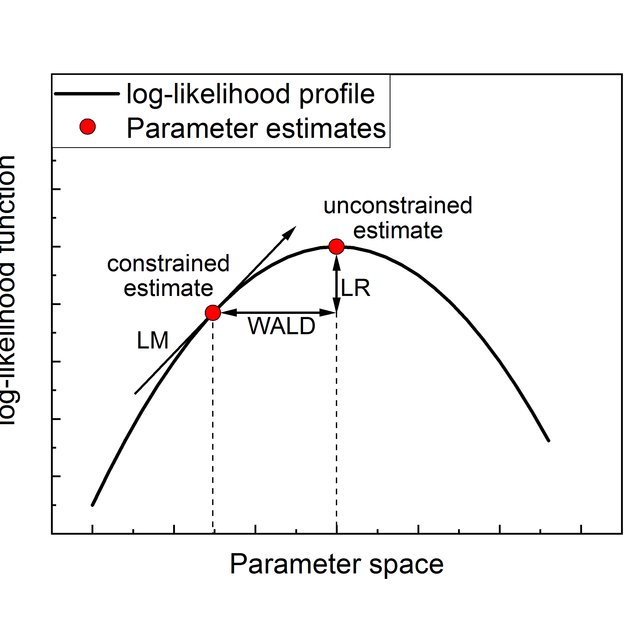
\includegraphics{img/wald-lm-lr.jpg}

All those test statistics are distributed as a \(\chi^2\) distribution

MLE is also used for machine learning/econometrics, especially when relationships are non linear \(\Rightarrow\) logistic regression.

\textbf{Notes :}

\begin{itemize}
\tightlist
\item
  Sample mean is the MLE for the exponential family (eg gaussian distribution)
\item
  MLE is a subset of \href{https://en.wikipedia.org/wiki/M-estimator}{M-estimators}
\end{itemize}

\hypertarget{exercises-interprete-a-test-you-dont-know}{%
\subsection{Exercises : interprete a test you don't know}\label{exercises-interprete-a-test-you-dont-know}}

\begin{itemize}
\tightlist
\item
  Run a Kolmogorov--Smirnov test on the distance variable, and the logarithm of this variable. What can you conclude ?
\item
  In time series analysis, it is crucial to check if a time series is stationary or not. Stationarity means that both mean and variance are constant over time (no drift). If it's the case, it's easier to model it.
  To check that, there are several tests called ``unit-root'' tests (if there is a unit root, the serie is not stationary).
  In this example, I simulate a time series and run the Phillips-Perron test. The alternative hypothesis is specified in the output ; please interpret the result.
\end{itemize}

\begin{Shaded}
\begin{Highlighting}[]
\KeywordTok{library}\NormalTok{(tseries)}
\CommentTok{# generation of a random walk}
\NormalTok{Xt <-}\StringTok{ }\KeywordTok{cumsum}\NormalTok{(}\KeywordTok{rnorm}\NormalTok{(}\DecValTok{100}\NormalTok{))}
\KeywordTok{plot}\NormalTok{(Xt,}\DataTypeTok{type=}\StringTok{"l"}\NormalTok{,}\DataTypeTok{main=}\StringTok{"Random time serie"}\NormalTok{,}\DataTypeTok{col=}\StringTok{"blue"}\NormalTok{)}
\end{Highlighting}
\end{Shaded}

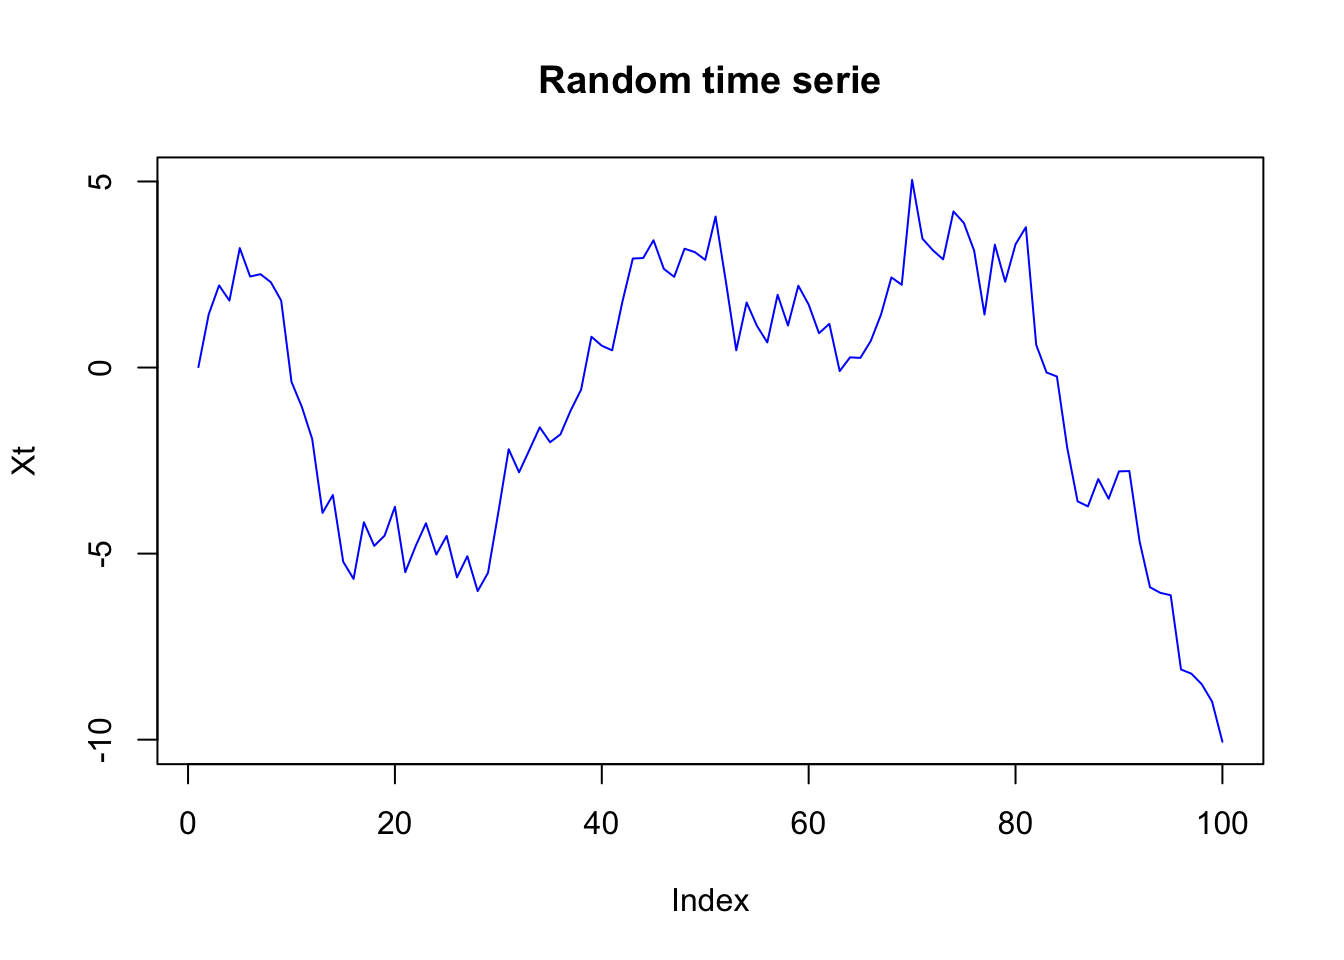
\includegraphics{DataExploration_files/figure-latex/unnamed-chunk-71-1.pdf}

\begin{Shaded}
\begin{Highlighting}[]
\KeywordTok{pp.test}\NormalTok{(Xt)}
\end{Highlighting}
\end{Shaded}

\begin{verbatim}
## 
## 	Phillips-Perron Unit Root Test
## 
## data:  Xt
## Dickey-Fuller Z(alpha) = -17.901, Truncation lag parameter = 3, p-value
## = 0.09351
## alternative hypothesis: stationary
\end{verbatim}

\hypertarget{multivariate-analysis-and-dimension-reduction}{%
\chapter{Multivariate analysis and dimension reduction}\label{multivariate-analysis-and-dimension-reduction}}

\hypertarget{multivar}{%
\section{Multivariate analysis}\label{multivar}}

\hypertarget{adv_viz}{%
\subsection{Advanced visualization}\label{adv_viz}}

\hypertarget{the-grammar-of-graphics}{%
\subsubsection{The grammar of graphics}\label{the-grammar-of-graphics}}

The grammar of graphics was introduced in 2005 by Wilkinson and Leland as a general framework for graphical representation of data. It was adapted by Hadley Wickham in the R package \texttt{ggplot2}.
\emph{It presents a unique foundation for producing almost every quantitative graphic found in scientific journals, newspapers, statistical packages, and data visualization systems}.

You can check \href{https://vita.had.co.nz/papers/layered-grammar.html}{the paper} from Wickham

When ploting data, one has to define :

\begin{itemize}
\tightlist
\item
  What are the aesthetics \(\rightarrow\) \textbf{the dimensions you want to represent}
\item
  What is the geometry you want to use \(\rightarrow\) \textbf{the kind of plot you want}
\item
  Ploting options (that come with default values) :

  \begin{itemize}
  \tightlist
  \item
    scales of the axis
  \item
    fonts and colors for text
  \item
    labels (title, axis titles\ldots)
  \end{itemize}
\end{itemize}

In short, what you have to find is the right combination of aesthetics and geometry that best represent the data. To find the recommended combination, don't forget to use \href{https://www.data-to-viz.com/}{From data to viz}

\hypertarget{playing-with-aesthetics}{%
\subsubsection{Playing with aesthetics}\label{playing-with-aesthetics}}

You must define at least 1 dimension for the plot, either continuous or categorical for the x axis. Then you can increase the number of dimensions (ie columns of the data frame) you want to represent :

\begin{itemize}
\tightlist
\item
  x and y for the axis
\item
  size : optional (integer) dimension that will represent an additional number
\item
  color/fill : optional (categorical) dimension reprensented by a color. Color is for line/point geoms, fill for bars/heatmap geoms
\item
  linetype : optional (categorical) : different type of lines (solid, dotted, dashed\ldots). Only for geometries using lines
\item
  shape : optional (categorical) : variable that will make the shape of the dot vary. Only for point geometries
\item
  alpha : optional (continuous) : the transparency of the dots (the lower the value, the more transparent the dot)
\item
  \ldots{}
\end{itemize}

More about the aesthetics \href{https://ggplot2.tidyverse.org/articles/ggplot2-specs.html}{here}

You can also use the \texttt{facet\_wrap()} or \texttt{facet\_grid()} functions to add up to 2 more dimensions with categorical variables (see demo)

\hypertarget{geometries}{%
\subsubsection{Geometries}\label{geometries}}

Once you chose the variables (dimensions) you want to plot, you have to chose the geometry, that highly depends on the type of variable (numerical or character/factor). Don't forget to reffer to the website \emph{from data to viz} if you need some inspiration.

A short list of most common geometries :

\begin{itemize}
\tightlist
\item
  geom\_bar for barplots
\item
  geom\_histogram for histograms
\item
  geom\_jitter for scatter plots
\item
  geom\_boxplot \& geom\_violin for compared density plots
\item
  geom\_tile for heatmaps
\item
  geom\_line for time series
\item
  geom\_text or geom\_label for text (annotations)
\item
  geom\_hline and geom\_vline for horizontal and vertiacal lines
\item
  \ldots\ldots{}
\end{itemize}

\begin{Shaded}
\begin{Highlighting}[]
\CommentTok{# From }
\KeywordTok{ggplot}\NormalTok{(dat_clean,}\KeywordTok{aes}\NormalTok{(}\DataTypeTok{x=}\NormalTok{distance)) }\OperatorTok{+}
\StringTok{  }\KeywordTok{theme_minimal}\NormalTok{()}
\end{Highlighting}
\end{Shaded}

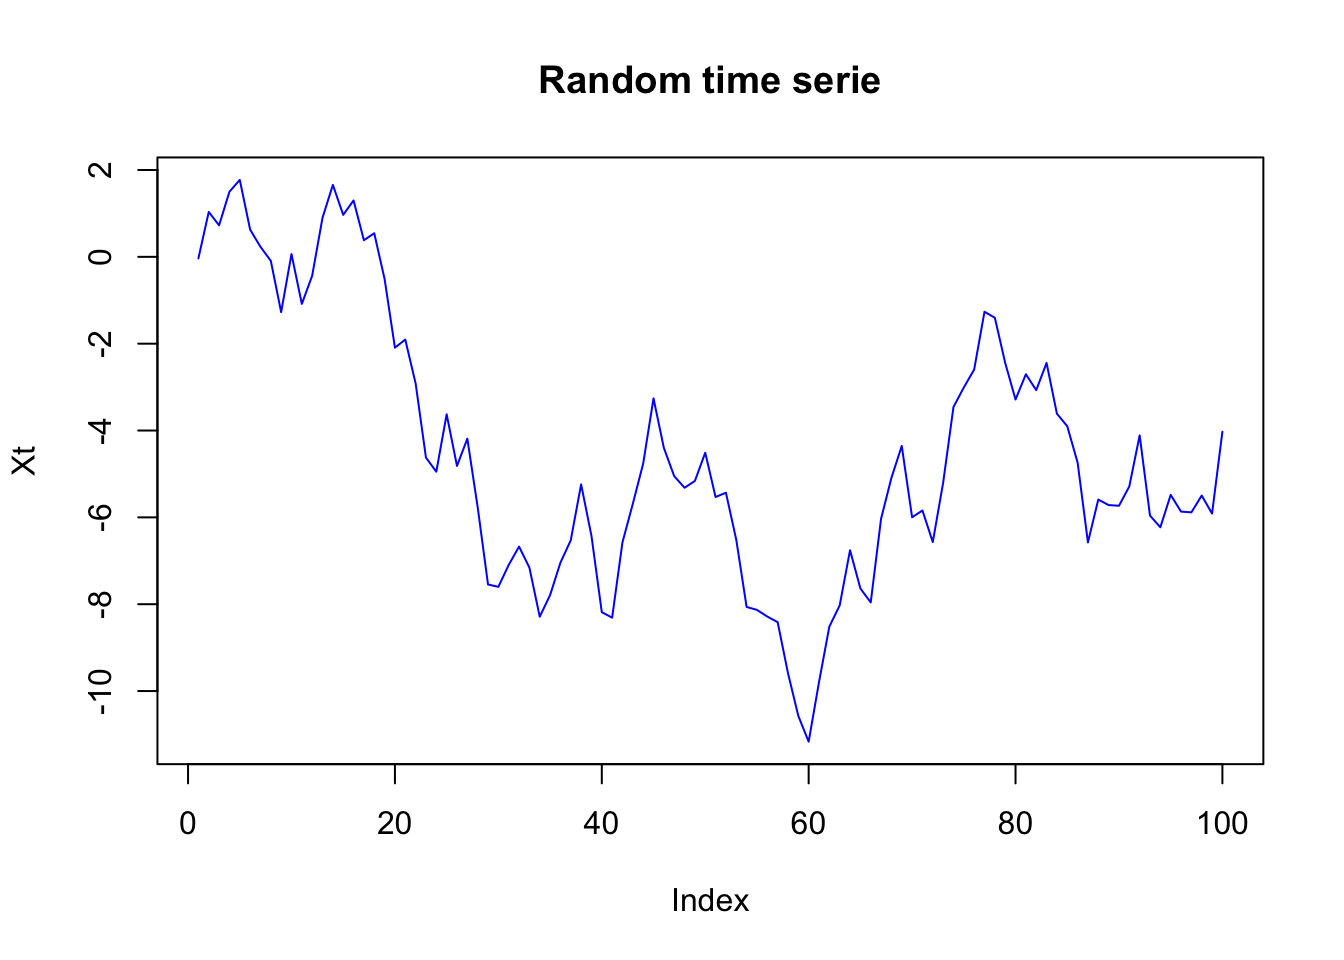
\includegraphics{DataExploration_files/figure-latex/unnamed-chunk-72-1.pdf}

\begin{Shaded}
\begin{Highlighting}[]
\KeywordTok{ggplot}\NormalTok{(dat_clean,}\KeywordTok{aes}\NormalTok{(}\DataTypeTok{x=}\NormalTok{distance)) }\OperatorTok{+}\StringTok{ }\KeywordTok{geom_histogram}\NormalTok{()}\OperatorTok{+}
\StringTok{  }\KeywordTok{theme_minimal}\NormalTok{()}
\end{Highlighting}
\end{Shaded}

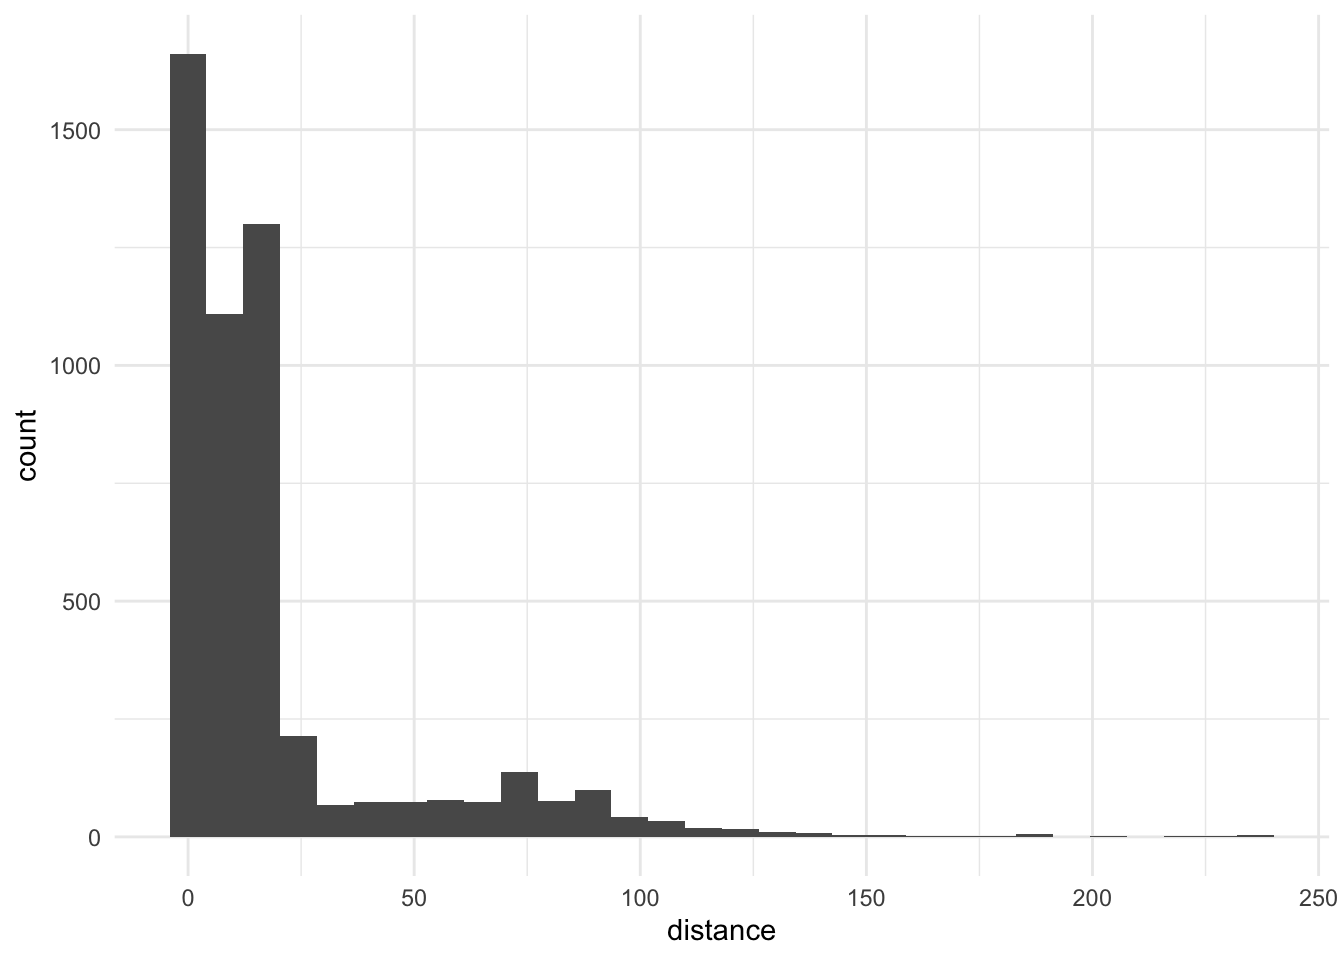
\includegraphics{DataExploration_files/figure-latex/unnamed-chunk-72-2.pdf}

\begin{Shaded}
\begin{Highlighting}[]
\KeywordTok{ggplot}\NormalTok{(dat_clean,}\KeywordTok{aes}\NormalTok{(distance,avgSpeed)) }\OperatorTok{+}\StringTok{ }\KeywordTok{geom_jitter}\NormalTok{()}\OperatorTok{+}
\StringTok{  }\KeywordTok{theme_minimal}\NormalTok{()}
\end{Highlighting}
\end{Shaded}

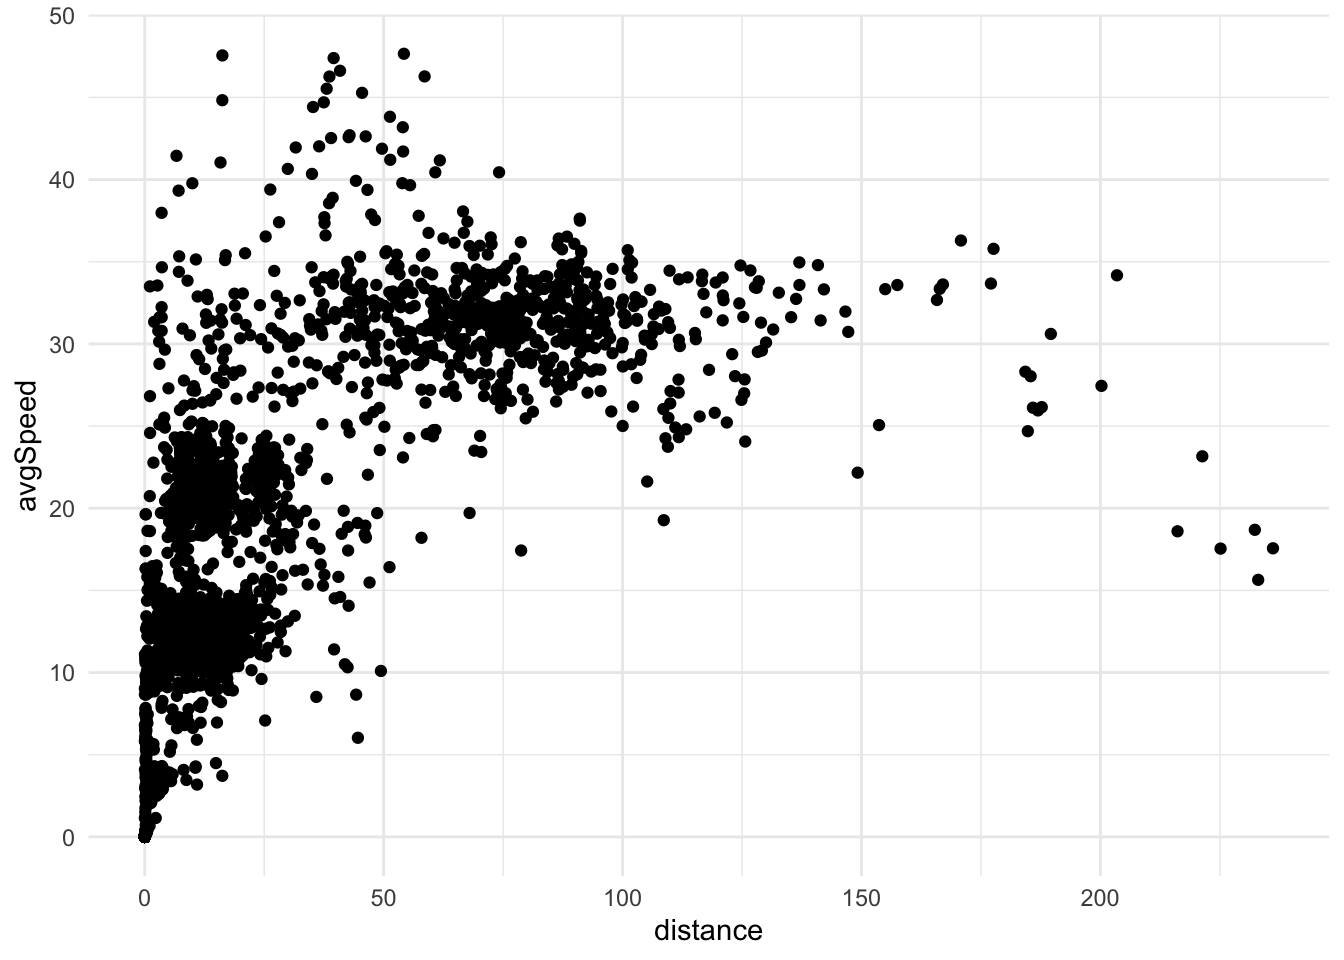
\includegraphics{DataExploration_files/figure-latex/unnamed-chunk-72-3.pdf}

\begin{Shaded}
\begin{Highlighting}[]
\KeywordTok{ggplot}\NormalTok{(dat_clean,}\KeywordTok{aes}\NormalTok{(distance,avgSpeed,}\DataTypeTok{color=}\NormalTok{activity_recoded))  }\OperatorTok{+}\StringTok{ }\KeywordTok{geom_jitter}\NormalTok{()}\OperatorTok{+}
\StringTok{  }\KeywordTok{theme_minimal}\NormalTok{()}
\end{Highlighting}
\end{Shaded}

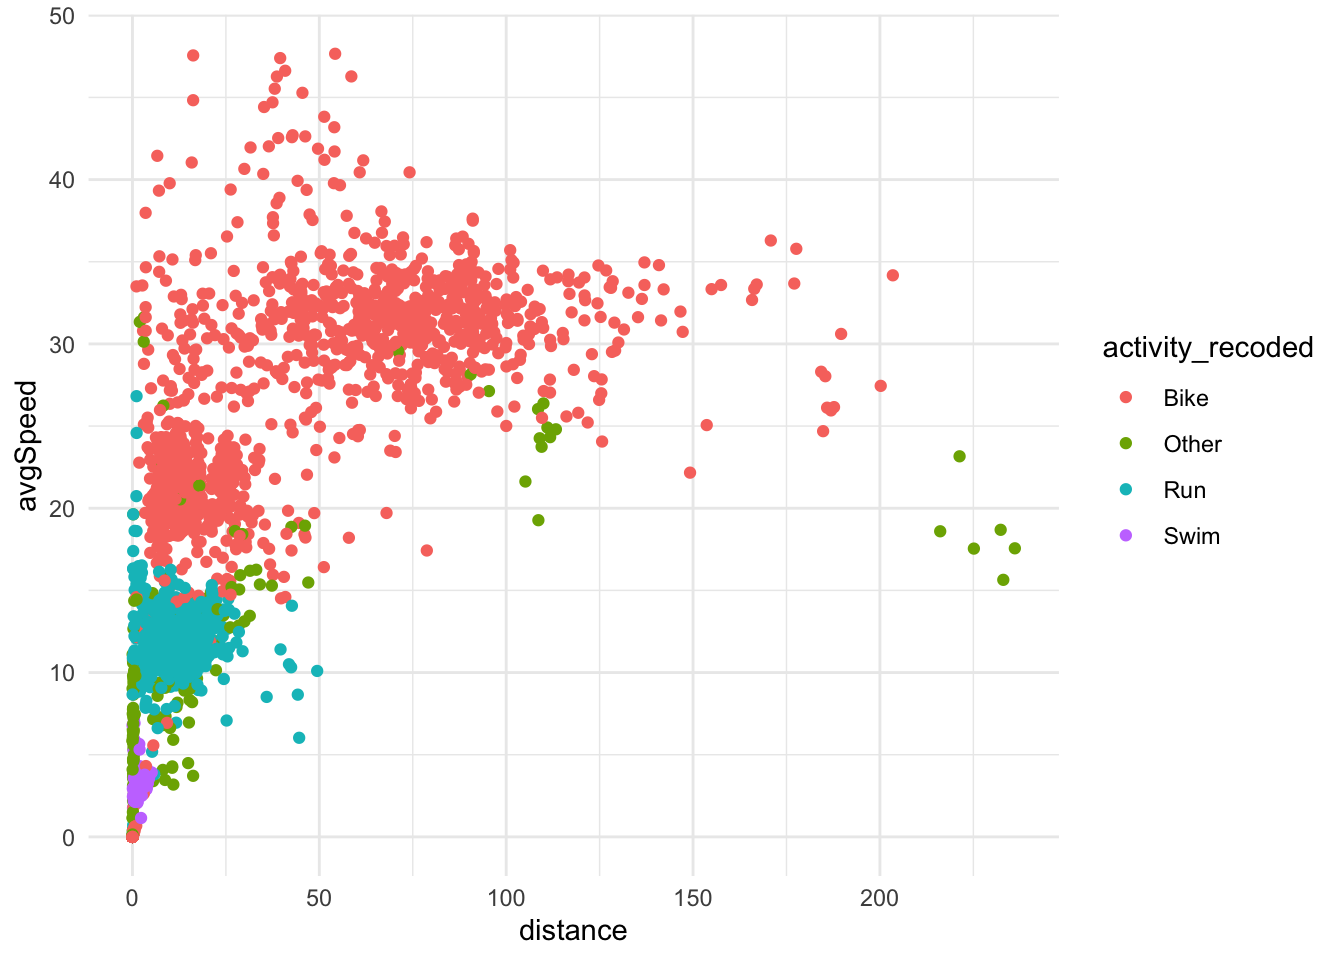
\includegraphics{DataExploration_files/figure-latex/unnamed-chunk-72-4.pdf}

\begin{Shaded}
\begin{Highlighting}[]
\CommentTok{# To }
\KeywordTok{ggplot}\NormalTok{(dat_clean,}\KeywordTok{aes}\NormalTok{(}\DataTypeTok{x=}\NormalTok{avgSpeed,}\DataTypeTok{y=}\NormalTok{calories,}\DataTypeTok{size=}\NormalTok{duration,}\DataTypeTok{color=}\NormalTok{qual_distance,}\DataTypeTok{shape=}\NormalTok{qual_avgHr)) }\OperatorTok{+}\StringTok{ }
\StringTok{  }\KeywordTok{geom_jitter}\NormalTok{() }\OperatorTok{+}\StringTok{ }
\StringTok{  }\KeywordTok{facet_wrap}\NormalTok{(.}\OperatorTok{~}\StringTok{ }\NormalTok{activity_recoded,}\DataTypeTok{scales =} \StringTok{"free"}\NormalTok{)}\OperatorTok{+}
\StringTok{  }\KeywordTok{theme_minimal}\NormalTok{()}
\end{Highlighting}
\end{Shaded}

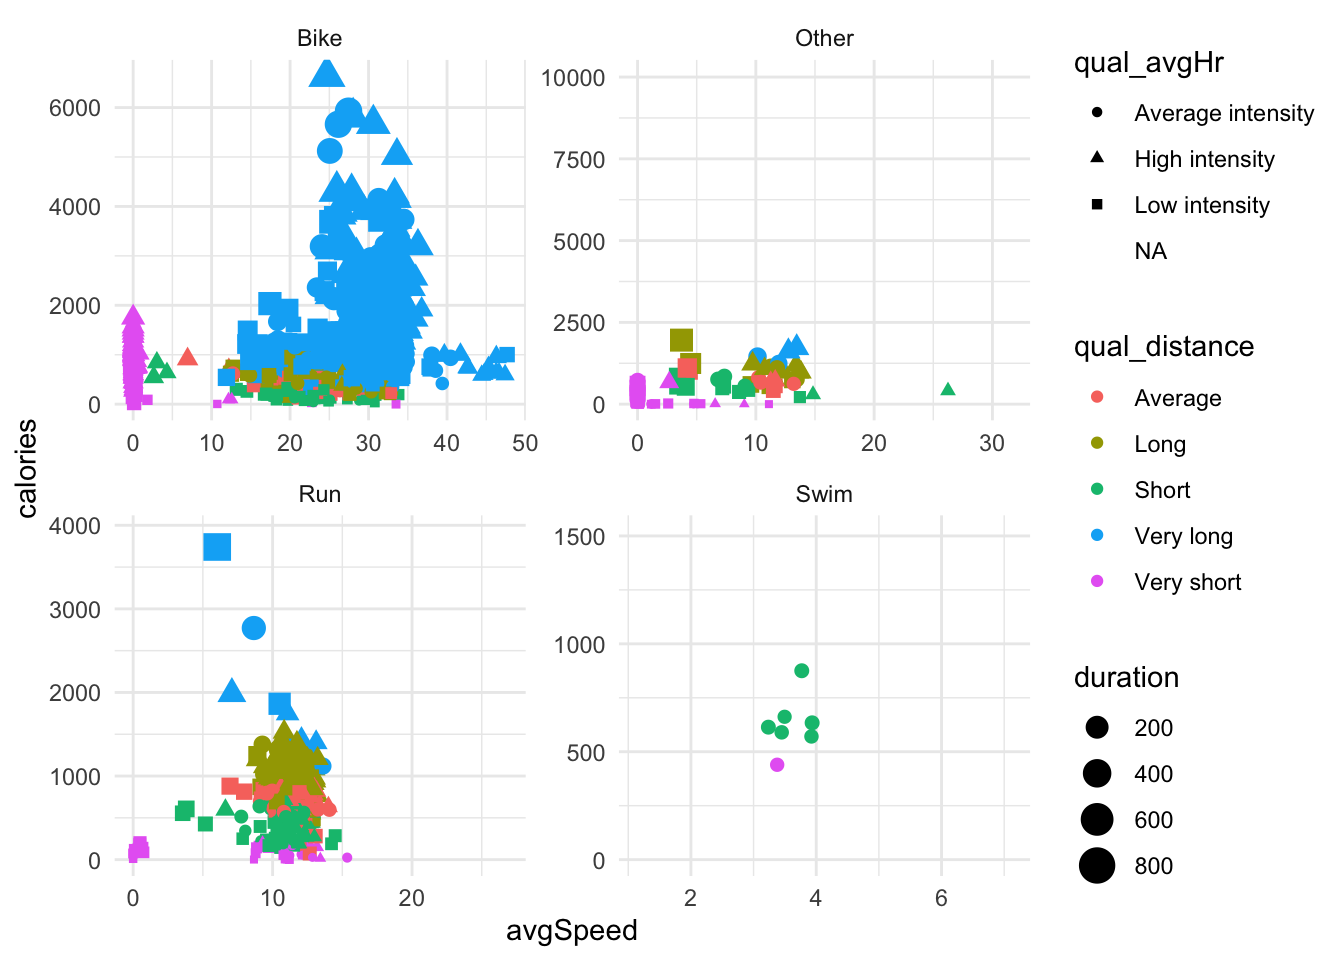
\includegraphics{DataExploration_files/figure-latex/unnamed-chunk-72-5.pdf}

\begin{Shaded}
\begin{Highlighting}[]
\CommentTok{# Or maybe}
\KeywordTok{ggplot}\NormalTok{(dat_clean,}\KeywordTok{aes}\NormalTok{(}\DataTypeTok{x=}\NormalTok{avgSpeed,}\DataTypeTok{y=}\NormalTok{elevationGain,}\DataTypeTok{size=}\NormalTok{calories,}\DataTypeTok{color=}\NormalTok{duration)) }\OperatorTok{+}\StringTok{ }
\StringTok{  }\KeywordTok{geom_jitter}\NormalTok{() }\OperatorTok{+}\StringTok{ }
\StringTok{  }\KeywordTok{facet_grid}\NormalTok{(activity_recoded}\OperatorTok{~}\NormalTok{qual_distance,}\DataTypeTok{scales =} \StringTok{"free"}\NormalTok{ )}\OperatorTok{+}
\StringTok{  }\KeywordTok{theme_minimal}\NormalTok{()}
\end{Highlighting}
\end{Shaded}

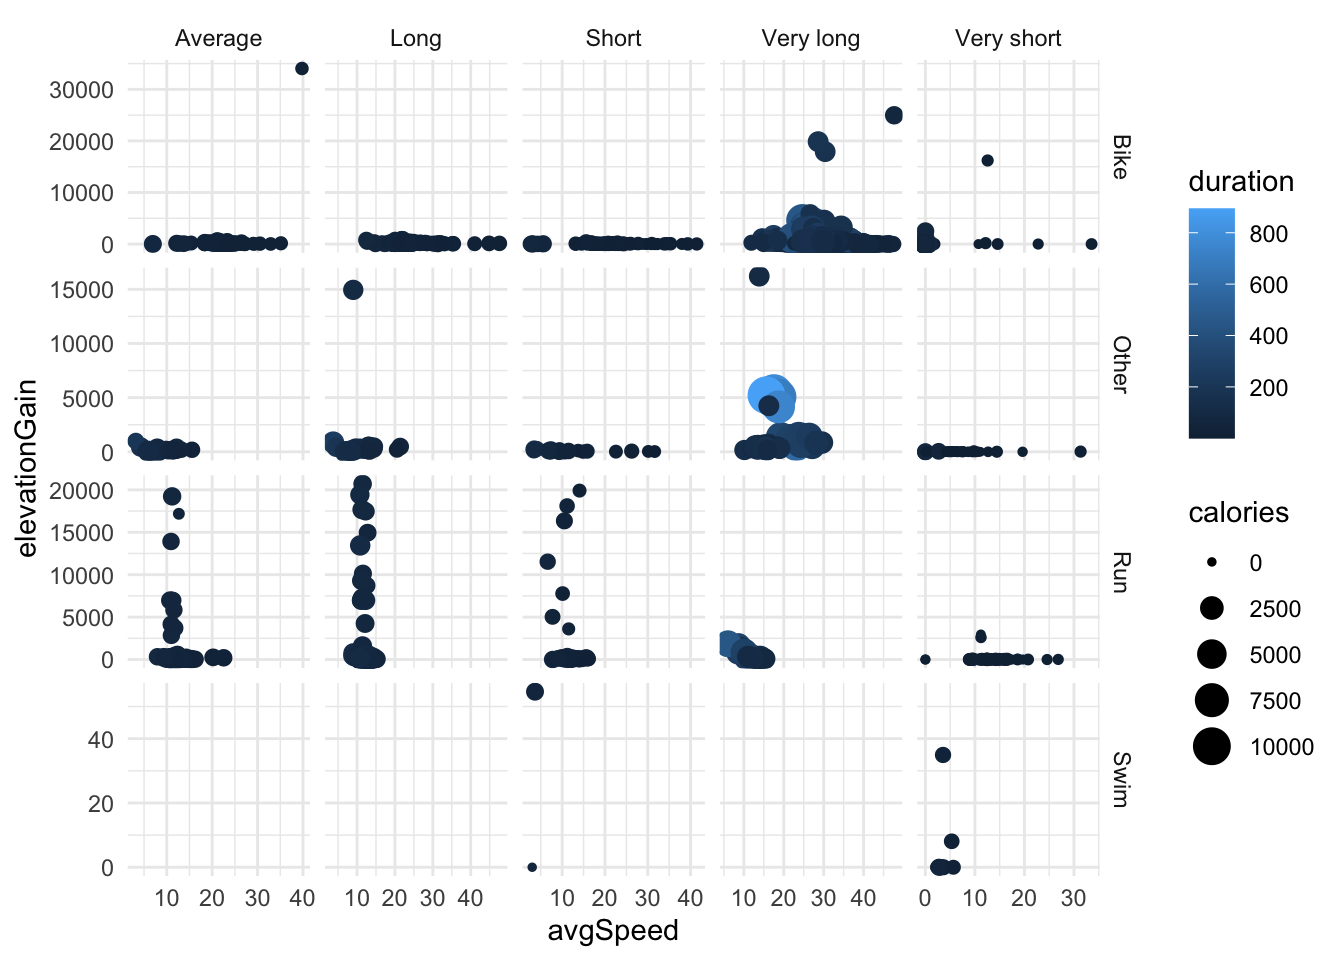
\includegraphics{DataExploration_files/figure-latex/unnamed-chunk-72-6.pdf}

\hypertarget{important-options}{%
\subsubsection{Important options}\label{important-options}}

With ggplot, one can make publishable graphics that don't need to be modified in another software. For that, the most useful functions are :

\begin{itemize}
\tightlist
\item
  scale\_xx\_yy : functions that allow you to tweak the axis' scale, the colors used by either \texttt{color} or \texttt{fill} aesthetics (eg : \texttt{scale\_color\_manual()}) and other options.
\item
  labs : allows you to proper label title, axis' titles, legend titles\ldots{}
\item
  theme : allows you to tweak general parameters for the plot (font family, font size, margins, background colors\ldots). You have several \texttt{theme\_xx()} functions already defined with different default values for those parameters (eg \texttt{theme\_minimal()} or \texttt{theme\_void()})
\item
  guides : allows you to modify the legend entries
\end{itemize}

Whats you can also do is recode the levels of the factor variables to make them more understanble or reorder them if you want them to be displayed in a specific order. See \texttt{forcats::fct\_recode()} and \texttt{forcats::fct\_reorder()}

\textbf{Hint :} when working with strings, you can force a string to be split in 2 rows with \texttt{\textbackslash{}n}

Here is an example :

\begin{Shaded}
\begin{Highlighting}[]
\NormalTok{dat_clean }\OperatorTok\StringTok{ }
\StringTok{  }\KeywordTok{ggplot}\NormalTok{(}\KeywordTok{aes}\NormalTok{(}\DataTypeTok{x=}\NormalTok{avgSpeed,}\DataTypeTok{y=}\NormalTok{elevationGain,}\DataTypeTok{size=}\NormalTok{calories,}\DataTypeTok{color=}\NormalTok{duration,}\DataTypeTok{size=}\NormalTok{distance)) }\OperatorTok{+}\StringTok{ }
\StringTok{  }\KeywordTok{geom_jitter}\NormalTok{() }\OperatorTok{+}\StringTok{ }
\StringTok{  }\KeywordTok{facet_grid}\NormalTok{(activity_recoded}\OperatorTok{~}\NormalTok{qual_distance,}\DataTypeTok{scales =} \StringTok{"free"}\NormalTok{ ) }\OperatorTok{+}
\StringTok{  }\KeywordTok{theme_minimal}\NormalTok{() }\OperatorTok{+}
\StringTok{  }\KeywordTok{labs}\NormalTok{(}\DataTypeTok{title=}\StringTok{"Great insights"}\NormalTok{,}\DataTypeTok{y=}\StringTok{"Total evelation"}\NormalTok{,}\DataTypeTok{x=}\StringTok{"Average speed"}\NormalTok{,}
       \DataTypeTok{color=}\StringTok{"Duration"}\NormalTok{,}\DataTypeTok{size=}\StringTok{"Total distance"}\NormalTok{) }\OperatorTok{+}
\StringTok{  }\CommentTok{# scale_color_manual(values = c("magenta","orange")) + }
\StringTok{  }\KeywordTok{scale_size_continuous}\NormalTok{(}\DataTypeTok{labels=}\NormalTok{scales}\OperatorTok{::}\NormalTok{comma) }\OperatorTok{+}
\StringTok{  }\KeywordTok{scale_y_continuous}\NormalTok{(}\DataTypeTok{labels=}\NormalTok{scales}\OperatorTok{::}\NormalTok{comma) }\OperatorTok{+}
\StringTok{  }\KeywordTok{scale_x_continuous}\NormalTok{(}\DataTypeTok{labels=}\NormalTok{scales}\OperatorTok{::}\NormalTok{comma)}\OperatorTok{+}
\StringTok{  }\KeywordTok{theme_minimal}\NormalTok{()}
\end{Highlighting}
\end{Shaded}

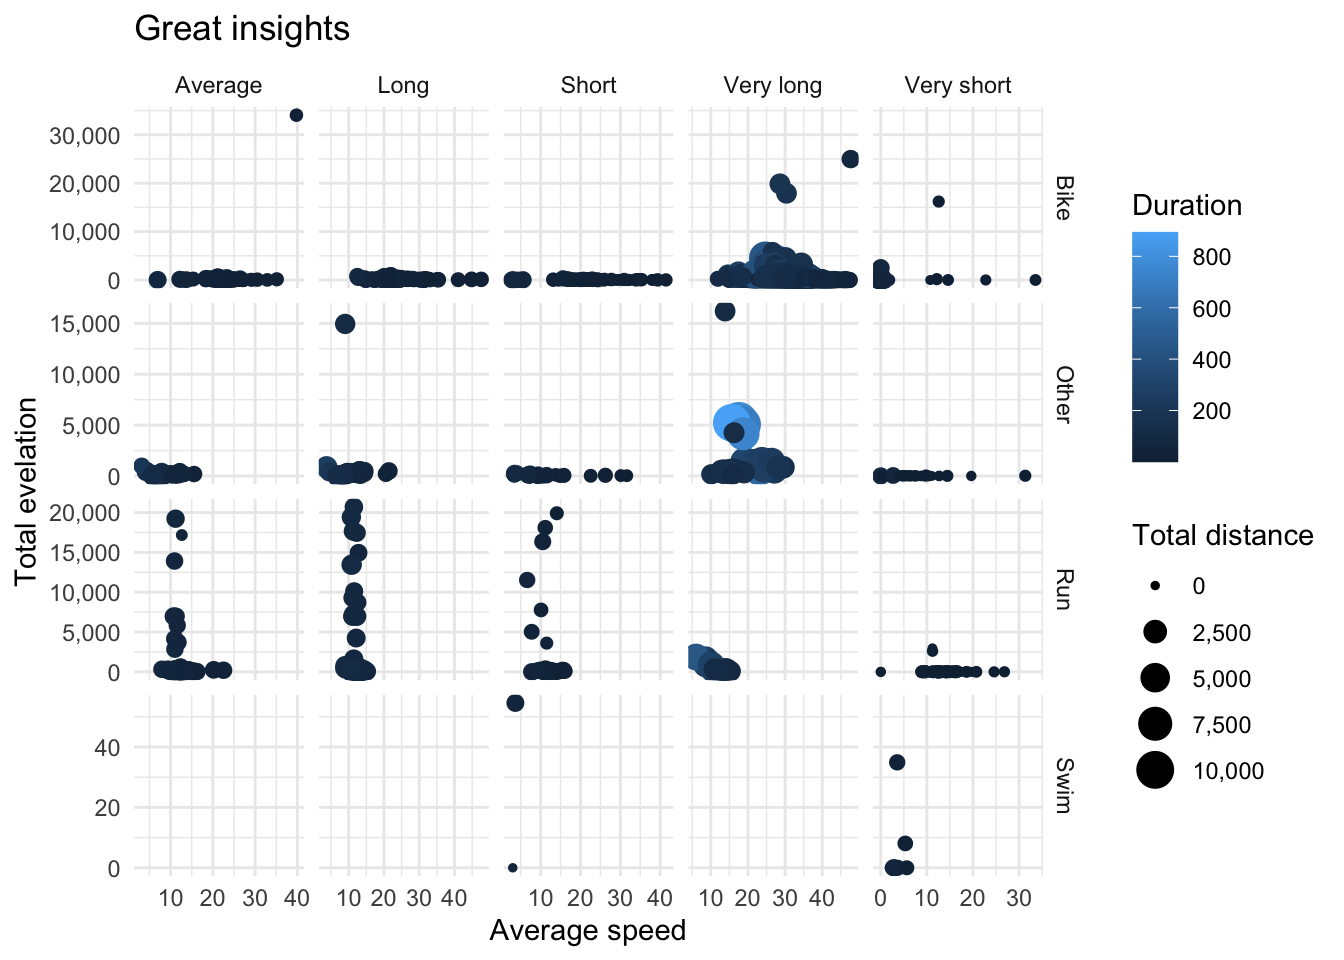
\includegraphics{DataExploration_files/figure-latex/unnamed-chunk-73-1.pdf}

\hypertarget{some-tricks-with-ggplot}{%
\subsubsection{Some tricks with ggplot}\label{some-tricks-with-ggplot}}

This approach (grammar of graphics) is very coherent but makes it sometimes difficult. For example, how can I represent the distribution of several variables (and not the distribution of one variable according to different sub-groups -meaning that there is a second dimension -) ?

\hypertarget{the-cheater-way}{%
\paragraph{The cheater way}\label{the-cheater-way}}

You can brute-force the graph by superposing different geometries. But first, you'll have to standardize the variables (they don't have the same scale). Remember the usage of \texttt{across} to apply a function to a selection of variables.

\begin{Shaded}
\begin{Highlighting}[]
\KeywordTok{mutate}\NormalTok{(dat_clean,}\KeywordTok{across}\NormalTok{(}\KeywordTok{where}\NormalTok{(is.numeric),}
                        \ControlFlowTok{function}\NormalTok{(xx) (xx}\OperatorTok{-}\KeywordTok{mean}\NormalTok{(xx,}\DataTypeTok{na.rm=}\NormalTok{T))}\OperatorTok{/}\KeywordTok{sd}\NormalTok{(xx,}\DataTypeTok{na.rm=}\NormalTok{T))) }\OperatorTok\StringTok{ }
\StringTok{  }\KeywordTok{ggplot}\NormalTok{() }\OperatorTok{+}\StringTok{ }\KeywordTok{geom_density}\NormalTok{(}\KeywordTok{aes}\NormalTok{(distance),}\DataTypeTok{color=}\StringTok{"blue"}\NormalTok{) }\OperatorTok{+}\StringTok{ }
\StringTok{  }\KeywordTok{geom_density}\NormalTok{(}\KeywordTok{aes}\NormalTok{(duration),}\DataTypeTok{color=}\StringTok{"red"}\NormalTok{)}\OperatorTok{+}
\StringTok{  }\KeywordTok{theme_minimal}\NormalTok{()}
\end{Highlighting}
\end{Shaded}

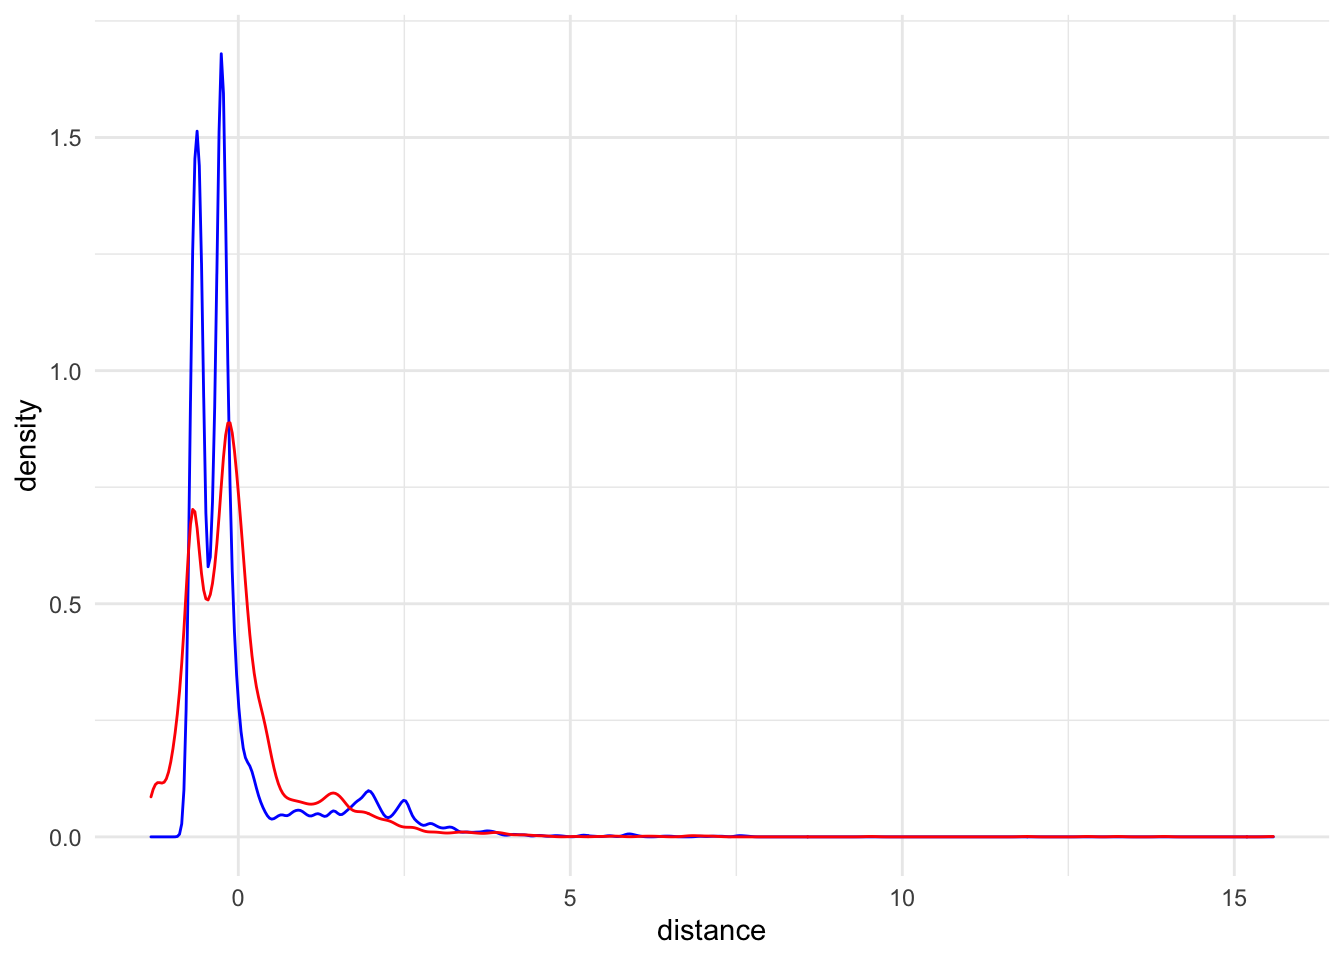
\includegraphics{DataExploration_files/figure-latex/unnamed-chunk-74-1.pdf}

This solution can be also used if you want to superpose different geometries (bars and lines, bars and hlines,\ldots), and is in this case legal :D

\hypertarget{do-it-with-the-tidy-philosophy}{%
\paragraph{Do it with the tidy philosophy}\label{do-it-with-the-tidy-philosophy}}

You can reformulate this task as : I want to represent the distribution of one unique variable for 2 subgroups : distance and duration. I have to reshape the data first to create such a variable. For that I will use \texttt{tidyr::pivot\_longer()} which helps me to transform columns into rows.

\begin{Shaded}
\begin{Highlighting}[]
\NormalTok{reshaped <-}\StringTok{ }\KeywordTok{select}\NormalTok{(dat_clean,duration,distance) }\OperatorTok\StringTok{ }
\StringTok{  }\KeywordTok{pivot_longer}\NormalTok{(}\DataTypeTok{cols =} \KeywordTok{everything}\NormalTok{(),}\DataTypeTok{names_to=}\StringTok{"latent_variable"}\NormalTok{,}\DataTypeTok{values_to=}\StringTok{"values"}\NormalTok{)}
\NormalTok{reshaped}
\end{Highlighting}
\end{Shaded}

\begin{verbatim}
## # A tibble: 10,250 x 2
##    latent_variable values
##    <chr>            <dbl>
##  1 duration          60.7
##  2 distance           3  
##  3 duration         251. 
##  4 distance         123. 
##  5 duration         173. 
##  6 distance          83.6
##  7 duration          89.9
##  8 distance          17.9
##  9 duration          60.4
## 10 distance          34.9
## # ... with 10,240 more rows
\end{verbatim}

Now I can use the latent\_variable variable as a dimension in a classic ggplot statement, with a prior standardization

\begin{Shaded}
\begin{Highlighting}[]
\KeywordTok{group_by}\NormalTok{(reshaped,latent_variable) }\OperatorTok\StringTok{ }
\StringTok{  }\KeywordTok{mutate}\NormalTok{(}\DataTypeTok{values=}\NormalTok{(values}\OperatorTok{-}\KeywordTok{mean}\NormalTok{(values,}\DataTypeTok{na.rm =}\NormalTok{ T))}\OperatorTok{/}\KeywordTok{sd}\NormalTok{(values,}\DataTypeTok{na.rm =}\NormalTok{ T)) }\OperatorTok\StringTok{ }
\StringTok{  }\KeywordTok{ggplot}\NormalTok{(}\KeywordTok{aes}\NormalTok{(values,}\DataTypeTok{color=}\NormalTok{latent_variable)) }\OperatorTok{+}\StringTok{ }\KeywordTok{geom_histogram}\NormalTok{()}\OperatorTok{+}
\StringTok{  }\KeywordTok{theme_minimal}\NormalTok{()}
\end{Highlighting}
\end{Shaded}

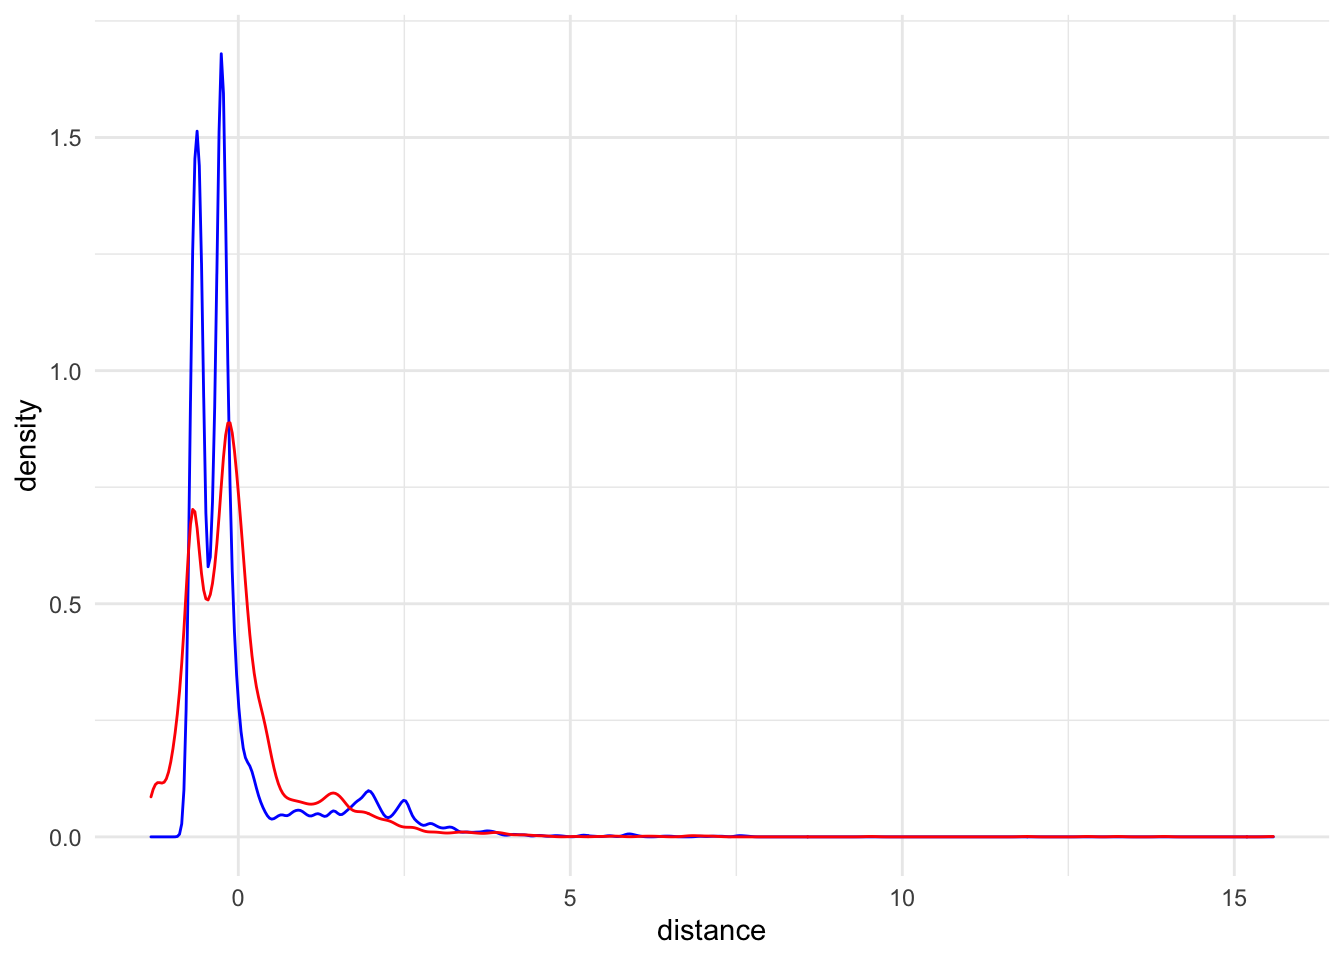
\includegraphics{DataExploration_files/figure-latex/unnamed-chunk-76-1.pdf}

Or you can even skip the standardization step thanks to facets :

\begin{Shaded}
\begin{Highlighting}[]
\KeywordTok{ggplot}\NormalTok{(reshaped,}\KeywordTok{aes}\NormalTok{(values)) }\OperatorTok{+}\StringTok{ }\KeywordTok{geom_histogram}\NormalTok{() }\OperatorTok{+}\StringTok{ }
\StringTok{  }\KeywordTok{facet_wrap}\NormalTok{(.}\OperatorTok{~}\NormalTok{latent_variable,}\DataTypeTok{scales =} \StringTok{"free"}\NormalTok{)}\OperatorTok{+}
\StringTok{  }\KeywordTok{theme_minimal}\NormalTok{()}
\end{Highlighting}
\end{Shaded}

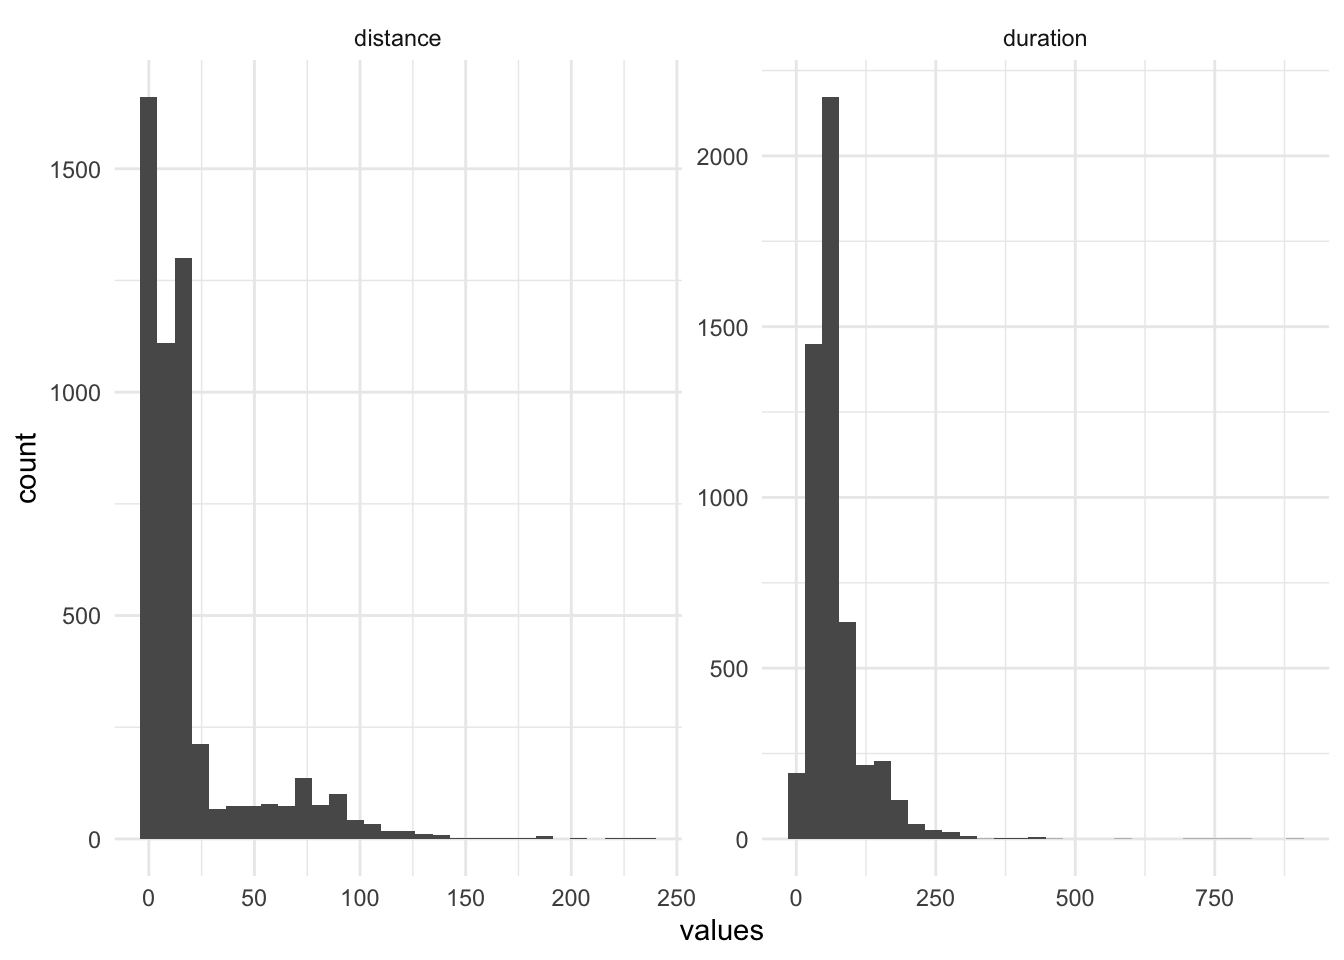
\includegraphics{DataExploration_files/figure-latex/unnamed-chunk-77-1.pdf}

\hypertarget{combine-different-plots-with-ggpubr}{%
\paragraph{Combine different plots with ggpubr}\label{combine-different-plots-with-ggpubr}}

\texttt{ggpubr} makes your life much easier to make publication-ready graphics. It allows you for example to combine several ggplot graphics in a grid, regardless of any latent dimension that facet\_grid would require. For that you have to store the graphics and ``replay'' them in a defined grid generated by \texttt{ggarrange()}

\begin{Shaded}
\begin{Highlighting}[]
\CommentTok{# install.packages("ggpubr")}
\KeywordTok{require}\NormalTok{(ggpubr)}
\NormalTok{gg1 <-}\StringTok{ }\KeywordTok{ggplot}\NormalTok{(dat_clean,}\KeywordTok{aes}\NormalTok{(distance)) }\OperatorTok{+}\StringTok{ }\KeywordTok{geom_histogram}\NormalTok{() }\OperatorTok{+}\StringTok{ }\KeywordTok{labs}\NormalTok{(}\DataTypeTok{title =} \StringTok{"Distance distribution"}\NormalTok{)}\OperatorTok{+}
\StringTok{  }\KeywordTok{theme_minimal}\NormalTok{()}
\NormalTok{gg2 <-}\StringTok{ }\KeywordTok{ggplot}\NormalTok{(dat_clean,}\KeywordTok{aes}\NormalTok{(}\DataTypeTok{x=}\NormalTok{avgSpeed,}\DataTypeTok{y=}\NormalTok{elevationGain,}\DataTypeTok{size=}\NormalTok{calories,}\DataTypeTok{color=}\NormalTok{duration,}\DataTypeTok{size=}\NormalTok{distance)) }\OperatorTok{+}\StringTok{ }
\StringTok{  }\KeywordTok{geom_jitter}\NormalTok{() }\OperatorTok{+}\StringTok{ }
\StringTok{  }\KeywordTok{facet_grid}\NormalTok{(activity_recoded}\OperatorTok{~}\NormalTok{qual_distance,}\DataTypeTok{scales =} \StringTok{"free"}\NormalTok{ ) }\OperatorTok{+}
\StringTok{  }\KeywordTok{theme_minimal}\NormalTok{() }\OperatorTok{+}\StringTok{ }\KeywordTok{labs}\NormalTok{(}\DataTypeTok{title =} \StringTok{"Beautiful but useless plot"}\NormalTok{)}\OperatorTok{+}
\StringTok{  }\KeywordTok{theme_minimal}\NormalTok{()}

\KeywordTok{ggarrange}\NormalTok{(gg1,gg2,}\DataTypeTok{ncol =} \DecValTok{2}\NormalTok{,}\DataTypeTok{widths =} \KeywordTok{c}\NormalTok{(}\DecValTok{1}\NormalTok{,}\DecValTok{2}\NormalTok{))}
\end{Highlighting}
\end{Shaded}

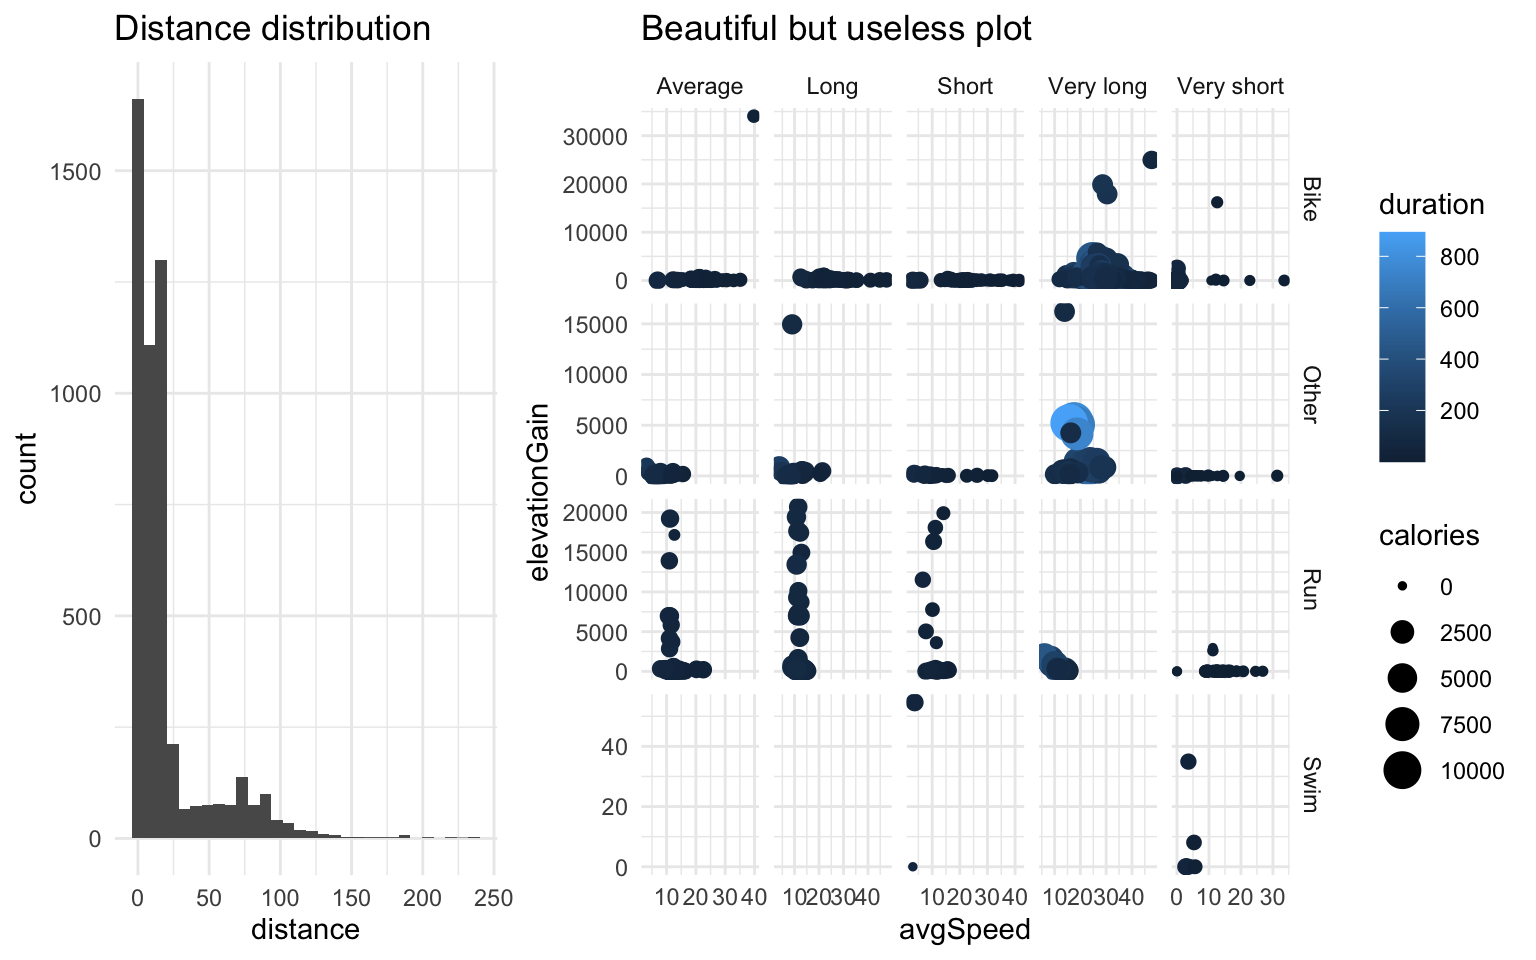
\includegraphics{DataExploration_files/figure-latex/unnamed-chunk-78-1.pdf}

There are a lot of options in this function (common legend, height and width of each plot,\ldots). You can check the full \href{http://www.sthda.com/english/articles/24-ggpubr-publication-ready-plots/}{documentation of this package}.

Note that you can mix tables and graphics with this function. Tables can be rendered as ggplot object with \texttt{ggpubr::ggtexttable()}

\hypertarget{easily-explore-an-entire-dataset}{%
\subsection{Easily explore an entire dataset}\label{easily-explore-an-entire-dataset}}

Now, you know how to produce one graph including several dimensions. To explore a new dataset and identify the correlations between them, you can visualize at a glance all variables in a datasets and their correlations with \texttt{GGally}

\hypertarget{scatter-plot-matrix}{%
\subsubsection{Scatter plot matrix}\label{scatter-plot-matrix}}

The scatter plot matrix shows the correlations between all variables and helps you to spot dependencies between them. We can use either the basic \texttt{plot()} function on the dataframe or the GGally package which provides nice extensions to ggplot.
Side note : the \texttt{ggpairs()} function does a lot of computation and can take a lot of time ! \(\rightarrow\) if your dataset is large, you should run it only on a sample of the observations with \texttt{dplyr::sample\_n()} or \texttt{dplyr::sample\_frac()} or only on a selection of columns.

\begin{Shaded}
\begin{Highlighting}[]
\KeywordTok{select}\NormalTok{(dat_clean,distance,duration,avgHr,avgSpeed,avgPower,}
\NormalTok{       calories,elevationGain,avgBikeCadence,activity_recoded) }\OperatorTok\StringTok{ }
\StringTok{  }\KeywordTok{plot}\NormalTok{()}
\end{Highlighting}
\end{Shaded}

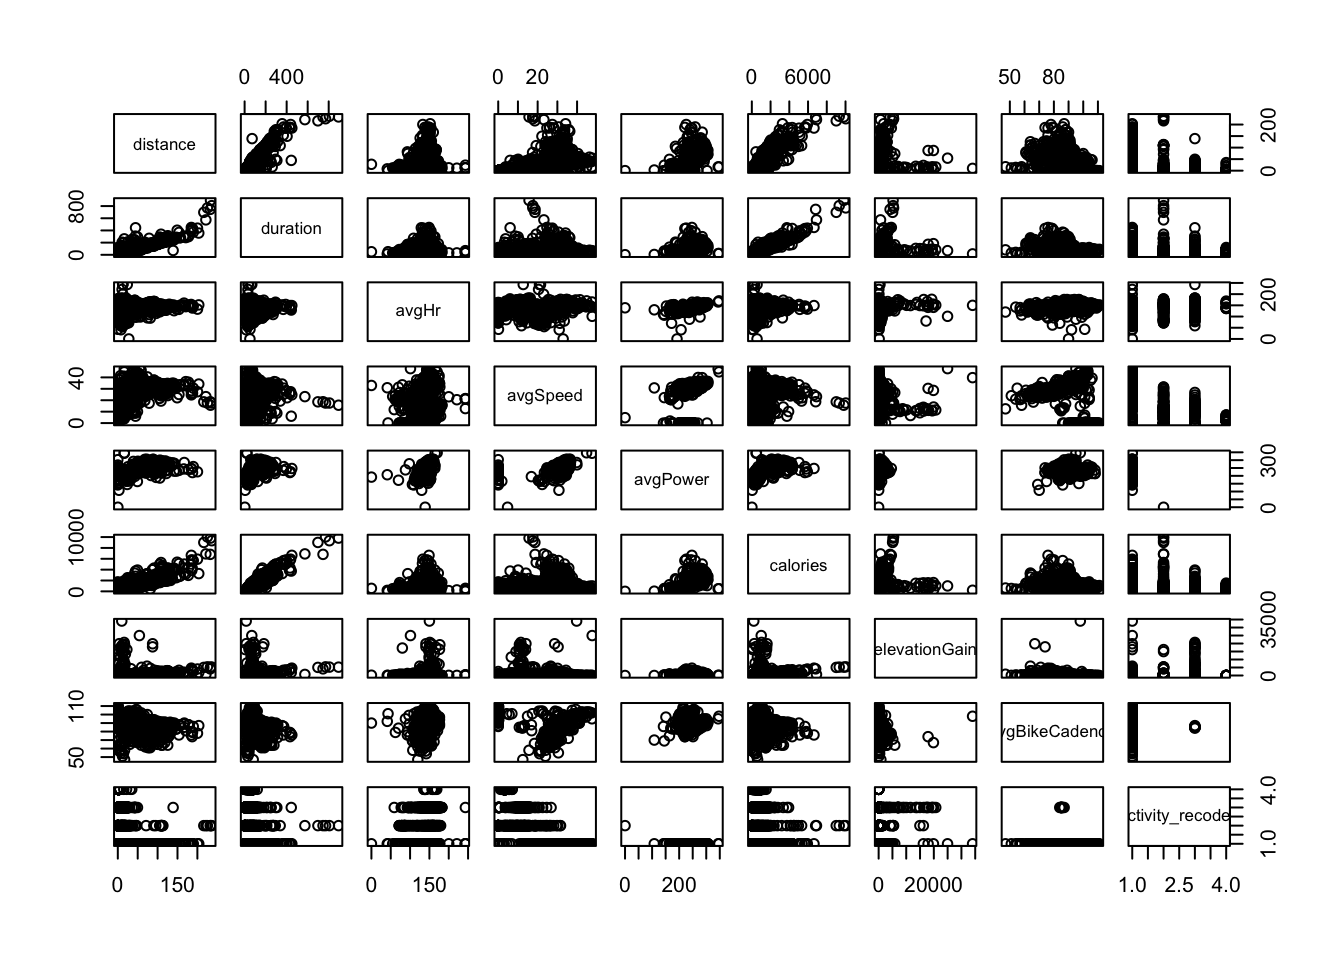
\includegraphics{DataExploration_files/figure-latex/unnamed-chunk-79-1.pdf}

\begin{Shaded}
\begin{Highlighting}[]
\CommentTok{# install.packages("GGally")}
\KeywordTok{require}\NormalTok{(GGally)}
\KeywordTok{select}\NormalTok{(dat_clean,distance,duration,avgSpeed,}
\NormalTok{       calories,activity_recoded) }\OperatorTok\StringTok{ }
\StringTok{  }\NormalTok{GGally}\OperatorTok{::}\KeywordTok{ggpairs}\NormalTok{()}
\end{Highlighting}
\end{Shaded}

\includegraphics{DataExploration_files/figure-latex/unnamed-chunk-79-2.pdf}

\hypertarget{correlation-plots}{%
\subsubsection{Correlation plots}\label{correlation-plots}}

\begin{Shaded}
\begin{Highlighting}[]
\KeywordTok{select}\NormalTok{(dat_clean,distance,duration,avgHr,avgSpeed,avgPower,}
\NormalTok{       calories,elevationGain,avgDoubleCadence,activity_recoded)  }\OperatorTok\StringTok{ }
\StringTok{  }\NormalTok{GGally}\OperatorTok{::}\KeywordTok{ggcorr}\NormalTok{(}\DataTypeTok{geom =} \StringTok{"circle"}\NormalTok{)}
\end{Highlighting}
\end{Shaded}

\includegraphics{DataExploration_files/figure-latex/unnamed-chunk-80-1.pdf}

\hypertarget{multivariate-analysis-and-dimension-reduction-1}{%
\section{Multivariate analysis and dimension reduction}\label{multivariate-analysis-and-dimension-reduction-1}}

In this section, we will focus on the bike activities, which have the highest number of metrics. However, before we can go further, we have to deal with missing data and scale them to avoid that the column with a large order of magnitude are over-weighted.

\hypertarget{imputation}{%
\subsection{Imputation}\label{imputation}}

So far, we have ignored the missing values because we were computing summary statistics on one or 2 variables. The problem when taking into account more columns is that the probability of having one missing value on one of these features is higher, and therefore the risk that the whole observation is ignored increases. Every observation should still contain some original information that an analysis (or a model) should reflect. To avoid to ignore to many observations because of missing data we perform \textbf{imputation}, meaning that we replace the missing value with a true value. Many methods can be used to that end :

For numeric variables

\begin{itemize}
\tightlist
\item
  Imputation with a random value from the sample
\item
  Imputation with the mean/median
\item
  Imputation with the nearest neighbours (k-nn)
\item
  Hotdeck
\item
  Imputation with a model (regression)
\end{itemize}

For categorical variables :

\begin{itemize}
\tightlist
\item
  Imputation with random category selection
\item
  Imputation with the most frequent category (total or of the neighbours)
\item
  Hotdeck
\item
  Model-based imputation
\end{itemize}

The challenge here is to chose between ``reflecting the instance's originality'' or ``not creating noise''

The following code counts the number of missing values per column and does a simple mean or median imputation. We will practice hte imputation via regression in the final chapter's exercises.

\begin{Shaded}
\begin{Highlighting}[]
\NormalTok{dat_bike <-}\StringTok{ }\KeywordTok{filter}\NormalTok{(dat_clean,is_bike) }\CommentTok{# Bike activities}
\KeywordTok{sapply}\NormalTok{(dat_bike,}\ControlFlowTok{function}\NormalTok{(xx) }\KeywordTok{sum}\NormalTok{(}\KeywordTok{is.na}\NormalTok{(xx)))}
\end{Highlighting}
\end{Shaded}

\begin{verbatim}
##              activityId                 uuidMsb                 uuidLsb 
##                       0                     932                     932 
##                    name            activityType           userProfileId 
##                     229                       0                       0 
##              timeZoneId          beginTimestamp             eventTypeId 
##                       0                       0                       0 
##                    rule               sportType            startTimeGmt 
##                       0                    1262                       0 
##          startTimeLocal                duration                distance 
##                       0                       0                       1 
##           elevationGain           elevationLoss                avgSpeed 
##                     175                     176                       2 
##                maxSpeed                   avgHr                   maxHr 
##                     495                     665                     664 
##                calories          startLongitude           startLatitude 
##                       2                     583                     583 
##   aerobicTrainingEffect    avgFractionalCadence    maxFractionalCadence 
##                    1376                       0                       0 
##         elapsedDuration          movingDuration anaerobicTrainingEffect 
##                    1189                    1528                    2021 
##                deviceId          minTemperature          maxTemperature 
##                     852                    1000                    1000 
##            minElevation            maxElevation            locationName 
##                    1018                    1018                    1781 
##        maxVerticalSpeed                lapCount            endLongitude 
##                    1708                    1642                    2186 
##             endLatitude              activeSets               totalSets 
##                    2186                    1855                    1855 
##               totalReps              purposeful        autoCalcCalories 
##                    1855                       0                    1246 
##                favorite                      pr      elevationCorrected 
##                       0                       0                     871 
##             atpActivity                  parent           maxRunCadence 
##                    1828                     474                    2491 
##                   steps  avgVerticalOscillation    avgGroundContactTime 
##                    2491                    2492                    2492 
##         avgStrideLength             vO2MaxValue        avgVerticalRatio 
##                    2491                    2289                    2492 
## avgGroundContactBalance        avgDoubleCadence        maxDoubleCadence 
##                    2492                    2491                    2491 
##                avgPower          avgBikeCadence          maxBikeCadence 
##                    1832                    1188                    1188 
##                 strokes               normPower          avgLeftBalance 
##                    1197                    1832                    1896 
##         avgRightBalance           max20MinPower     trainingStressScore 
##                    1896                    1838                    1881 
##         intensityFactor     lactateThresholdBpm   lactateThresholdSpeed 
##                    1881                    2492                    2492 
##              avgStrokes           activeLengths                avgSwolf 
##                    2492                    2311                    2492 
##              poolLength       avgStrokeDistance          avgSwimCadence 
##                    2492                    2492                    2492 
##          maxSwimCadence                  maxFtp               workoutId 
##                    2492                    2435                    2381 
##                decoDive                parentId        avgVerticalSpeed 
##                    2492                    2479                    2492 
##                maxDepth                avgDepth         surfaceInterval 
##                    2492                    2492                    2492 
##         floorsDescended              bottomTime              start_time 
##                    2492                    2492                       0 
##                    date                 is_bike                  is_run 
##                       0                       0                       0 
##        activity_recoded           qual_distance              qual_avgHr 
##                       0                       0                     914
\end{verbatim}

For this use case, we will use a median imputation, because for some of the variables, the mean would not make sense (eg longitude and latitude).

\begin{Shaded}
\begin{Highlighting}[]
\NormalTok{dat_bike_imp <-}\StringTok{ }\KeywordTok{mutate}\NormalTok{(dat_bike,}\KeywordTok{across}\NormalTok{(}\KeywordTok{where}\NormalTok{(is.numeric),}
                                   \ControlFlowTok{function}\NormalTok{(xx) }\KeywordTok{ifelse}\NormalTok{(}\KeywordTok{is.na}\NormalTok{(xx),}\KeywordTok{median}\NormalTok{(xx,}\DataTypeTok{na.rm=}\NormalTok{T),xx)))}
\KeywordTok{sapply}\NormalTok{(dat_bike_imp,}\ControlFlowTok{function}\NormalTok{(xx) }\KeywordTok{sum}\NormalTok{(}\KeywordTok{is.na}\NormalTok{(xx)))}
\end{Highlighting}
\end{Shaded}

\begin{verbatim}
##              activityId                 uuidMsb                 uuidLsb 
##                       0                     932                     932 
##                    name            activityType           userProfileId 
##                     229                       0                       0 
##              timeZoneId          beginTimestamp             eventTypeId 
##                       0                       0                       0 
##                    rule               sportType            startTimeGmt 
##                       0                    1262                       0 
##          startTimeLocal                duration                distance 
##                       0                       0                       0 
##           elevationGain           elevationLoss                avgSpeed 
##                       0                       0                       0 
##                maxSpeed                   avgHr                   maxHr 
##                       0                       0                       0 
##                calories          startLongitude           startLatitude 
##                       0                       0                       0 
##   aerobicTrainingEffect    avgFractionalCadence    maxFractionalCadence 
##                       0                       0                       0 
##         elapsedDuration          movingDuration anaerobicTrainingEffect 
##                       0                       0                       0 
##                deviceId          minTemperature          maxTemperature 
##                     852                       0                       0 
##            minElevation            maxElevation            locationName 
##                       0                       0                    1781 
##        maxVerticalSpeed                lapCount            endLongitude 
##                       0                       0                       0 
##             endLatitude              activeSets               totalSets 
##                       0                       0                       0 
##               totalReps              purposeful        autoCalcCalories 
##                       0                       0                    1246 
##                favorite                      pr      elevationCorrected 
##                       0                       0                       0 
##             atpActivity                  parent           maxRunCadence 
##                    1828                     474                       0 
##                   steps  avgVerticalOscillation    avgGroundContactTime 
##                       0                    2492                    2492 
##         avgStrideLength             vO2MaxValue        avgVerticalRatio 
##                    2491                       0                    2492 
## avgGroundContactBalance        avgDoubleCadence        maxDoubleCadence 
##                    2492                       0                       0 
##                avgPower          avgBikeCadence          maxBikeCadence 
##                       0                       0                       0 
##                 strokes               normPower          avgLeftBalance 
##                       0                       0                       0 
##         avgRightBalance           max20MinPower     trainingStressScore 
##                       0                       0                       0 
##         intensityFactor     lactateThresholdBpm   lactateThresholdSpeed 
##                       0                    2492                    2492 
##              avgStrokes           activeLengths                avgSwolf 
##                    2492                       0                    2492 
##              poolLength       avgStrokeDistance          avgSwimCadence 
##                    2492                    2492                    2492 
##          maxSwimCadence                  maxFtp               workoutId 
##                    2492                       0                    2381 
##                decoDive                parentId        avgVerticalSpeed 
##                    2492                    2479                    2492 
##                maxDepth                avgDepth         surfaceInterval 
##                    2492                    2492                    2492 
##         floorsDescended              bottomTime              start_time 
##                    2492                    2492                       0 
##                    date                 is_bike                  is_run 
##                       0                       0                       0 
##        activity_recoded           qual_distance              qual_avgHr 
##                       0                       0                     914
\end{verbatim}

Let's do the same for categorical (maximum frequency), even though it is not mandatory for PCA. We first have to create a function that will return the most frequent category of a vector.

\begin{Shaded}
\begin{Highlighting}[]
\NormalTok{most_freq_cat <-}\StringTok{ }\ControlFlowTok{function}\NormalTok{(xx)}
\NormalTok{\{}
\NormalTok{  tab <-}\StringTok{ }\KeywordTok{table}\NormalTok{(xx)}
  \KeywordTok{return}\NormalTok{(}\KeywordTok{names}\NormalTok{(tab[}\KeywordTok{which.max}\NormalTok{(tab)]))}
\NormalTok{\}}

\NormalTok{dat_bike_imp <-}\StringTok{ }\KeywordTok{mutate}\NormalTok{(dat_bike_imp,}\KeywordTok{across}\NormalTok{(}\KeywordTok{where}\NormalTok{(is.character),}
                                           \ControlFlowTok{function}\NormalTok{(xx) }\KeywordTok{coalesce}\NormalTok{(xx,}\KeywordTok{most_freq_cat}\NormalTok{(xx))))}

\KeywordTok{sapply}\NormalTok{(dat_bike_imp,}\ControlFlowTok{function}\NormalTok{(xx) }\KeywordTok{sum}\NormalTok{(}\KeywordTok{is.na}\NormalTok{(xx)))}
\end{Highlighting}
\end{Shaded}

\begin{verbatim}
##              activityId                 uuidMsb                 uuidLsb 
##                       0                       0                       0 
##                    name            activityType           userProfileId 
##                       0                       0                       0 
##              timeZoneId          beginTimestamp             eventTypeId 
##                       0                       0                       0 
##                    rule               sportType            startTimeGmt 
##                       0                       0                       0 
##          startTimeLocal                duration                distance 
##                       0                       0                       0 
##           elevationGain           elevationLoss                avgSpeed 
##                       0                       0                       0 
##                maxSpeed                   avgHr                   maxHr 
##                       0                       0                       0 
##                calories          startLongitude           startLatitude 
##                       0                       0                       0 
##   aerobicTrainingEffect    avgFractionalCadence    maxFractionalCadence 
##                       0                       0                       0 
##         elapsedDuration          movingDuration anaerobicTrainingEffect 
##                       0                       0                       0 
##                deviceId          minTemperature          maxTemperature 
##                       0                       0                       0 
##            minElevation            maxElevation            locationName 
##                       0                       0                       0 
##        maxVerticalSpeed                lapCount            endLongitude 
##                       0                       0                       0 
##             endLatitude              activeSets               totalSets 
##                       0                       0                       0 
##               totalReps              purposeful        autoCalcCalories 
##                       0                       0                    1246 
##                favorite                      pr      elevationCorrected 
##                       0                       0                       0 
##             atpActivity                  parent           maxRunCadence 
##                    1828                     474                       0 
##                   steps  avgVerticalOscillation    avgGroundContactTime 
##                       0                    2492                    2492 
##         avgStrideLength             vO2MaxValue        avgVerticalRatio 
##                       0                       0                    2492 
## avgGroundContactBalance        avgDoubleCadence        maxDoubleCadence 
##                    2492                       0                       0 
##                avgPower          avgBikeCadence          maxBikeCadence 
##                       0                       0                       0 
##                 strokes               normPower          avgLeftBalance 
##                       0                       0                       0 
##         avgRightBalance           max20MinPower     trainingStressScore 
##                       0                       0                       0 
##         intensityFactor     lactateThresholdBpm   lactateThresholdSpeed 
##                       0                    2492                    2492 
##              avgStrokes           activeLengths                avgSwolf 
##                    2492                       0                    2492 
##              poolLength       avgStrokeDistance          avgSwimCadence 
##                    2492                    2492                    2492 
##          maxSwimCadence                  maxFtp               workoutId 
##                    2492                       0                       0 
##                decoDive                parentId        avgVerticalSpeed 
##                    2492                       0                    2492 
##                maxDepth                avgDepth         surfaceInterval 
##                    2492                    2492                    2492 
##         floorsDescended              bottomTime              start_time 
##                    2492                    2492                       0 
##                    date                 is_bike                  is_run 
##                       0                       0                       0 
##        activity_recoded           qual_distance              qual_avgHr 
##                       0                       0                       0
\end{verbatim}

\begin{Shaded}
\begin{Highlighting}[]
\CommentTok{# replacements <-   select(dat_bike_imp,activityId,where(is.character)) %>%}
\CommentTok{#   pivot_longer(-activityId,names_to="name",values_to="val") %>% }
\CommentTok{#   filter(!is.na(val)) %>% }
\CommentTok{#   group_by(name,val) %>% }
\CommentTok{#   summarise(cat_nb=n()) %>% }
\CommentTok{#   arrange(name,-cat_nb) %>% }
\CommentTok{#   group_by(name) %>% }
\CommentTok{#   summarise(most_freq=first(val)) %>% }
\CommentTok{#   pivot_wider(names_from = name,values_from=most_freq) %>% }
\CommentTok{#   rename_with(function(xx) paste0(xx,"_imp"))}
\end{Highlighting}
\end{Shaded}

\hypertarget{normalization}{%
\subsection{Normalization}\label{normalization}}

Normalization is the operation consisting in scaling the columns so that their unit do not matter in the end. For example, the distance in meter is much larger than the cadence or the power, which have totally different units. To normalize the columns and make them unit-less, there are several methods among which the most common are the following :

\begin{itemize}
\tightlist
\item
  Standardization : \(X_i^{std} = \dfrac{X_i-\bar{X}}{\sigma_X} \rightarrow\) mean 0 and standard deviation 1
\item
  Min-Max scaling : \(X_i^{std} = \dfrac{X_i-min(X)}{max(X)-min(X)} \rightarrow\) between 0 and 1
\item
  Robust standardization \(X_i^{std} = \dfrac{X_i-Q2(X)}{Q3(X)-Q1(X)} \rightarrow\) similar to the first option but robust to outliers
\end{itemize}

You can check \href{https://scikit-learn.org/stable/modules/classes.html\#module-sklearn.preprocessing}{scikit-learn's documentation} to see what other options you have (and then search for their R implementation).

Normalization is a mandatory step before fitting a model, in order to avoid that only one feature bears the majority of the variance and makes the model biased.

\hypertarget{pca}{%
\subsection{PCA}\label{pca}}

Principal Components Analysis (PCA) is often seen by machine learning engineers ``only'' as a dimension reduction technique, but it is also a very powerful tool to explore your data. PCA applies on numerical variables only, and aims to \textbf{create new synthetic and uncorrelated variables : principal components} (as a linear combination of the original variables) such that the \emph{inertia} (ie variance) is highly concentrated on a small number of variables.

The mathematical problem is to find eigenvalues and eigenvectors of the correlation matrix. The eigenvectors represent the linear combination of the original variables needed to design those new variables, and the eigenvalues the variance that each of these new value bears. Once those new variables have been found, graphical representations within a few dimensions are possible.

To apply PCA, we will use the \texttt{FactoMineR} package, very easy to use for multivariate analysis.

\textbf{Notes} :

\begin{itemize}
\tightlist
\item
  You can have supplementary continuous or categorical variables. They won't be used in the construction of the eigenvectors, but you will be able to place them in the newly defined vector space.
\item
  By default, almost all implementations of PCA standardizes the data, so you do not have to do it by yourself, but check in the documentation of the function you use
\end{itemize}

\begin{Shaded}
\begin{Highlighting}[]
\CommentTok{# install.packages("FactoMineR")}
\KeywordTok{require}\NormalTok{(FactoMineR)}
\NormalTok{acp_dat <-}\StringTok{ }\KeywordTok{select}\NormalTok{(dat_bike_imp,deviceId,duration,distance,elevationGain,elevationLoss,avgSpeed,avgHr,calories,}
\NormalTok{              minTemperature,maxTemperature,lapCount,avgBikeCadence,avgPower,vO2MaxValue,}
\NormalTok{              max20MinPower) }
\NormalTok{acp <-}\StringTok{   }\KeywordTok{PCA}\NormalTok{(acp_dat,}\DataTypeTok{graph =}\NormalTok{ F,}\DataTypeTok{quali.sup =} \KeywordTok{c}\NormalTok{(}\DecValTok{1}\NormalTok{))}
\end{Highlighting}
\end{Shaded}

What's in this new object ?

\begin{Shaded}
\begin{Highlighting}[]
\KeywordTok{str}\NormalTok{(acp)}
\end{Highlighting}
\end{Shaded}

\begin{verbatim}
## List of 6
##  $ eig      : num [1:14, 1:3] 4.73 1.95 1.76 1.29 1.26 ...
##   ..- attr(*, "dimnames")=List of 2
##   .. ..$ : chr [1:14] "comp 1" "comp 2" "comp 3" "comp 4" ...
##   .. ..$ : chr [1:3] "eigenvalue" "percentage of variance" "cumulative percentage of variance"
##  $ var      :List of 4
##   ..$ coord  : num [1:14, 1:5] 0.799 0.902 0.495 0.507 0.658 ...
##   .. ..- attr(*, "dimnames")=List of 2
##   .. .. ..$ : chr [1:14] "duration" "distance" "elevationGain" "elevationLoss" ...
##   .. .. ..$ : chr [1:5] "Dim.1" "Dim.2" "Dim.3" "Dim.4" ...
##   ..$ cor    : num [1:14, 1:5] 0.799 0.902 0.495 0.507 0.658 ...
##   .. ..- attr(*, "dimnames")=List of 2
##   .. .. ..$ : chr [1:14] "duration" "distance" "elevationGain" "elevationLoss" ...
##   .. .. ..$ : chr [1:5] "Dim.1" "Dim.2" "Dim.3" "Dim.4" ...
##   ..$ cos2   : num [1:14, 1:5] 0.639 0.814 0.245 0.258 0.433 ...
##   .. ..- attr(*, "dimnames")=List of 2
##   .. .. ..$ : chr [1:14] "duration" "distance" "elevationGain" "elevationLoss" ...
##   .. .. ..$ : chr [1:5] "Dim.1" "Dim.2" "Dim.3" "Dim.4" ...
##   ..$ contrib: num [1:14, 1:5] 13.49 17.21 5.18 5.44 9.15 ...
##   .. ..- attr(*, "dimnames")=List of 2
##   .. .. ..$ : chr [1:14] "duration" "distance" "elevationGain" "elevationLoss" ...
##   .. .. ..$ : chr [1:5] "Dim.1" "Dim.2" "Dim.3" "Dim.4" ...
##  $ ind      :List of 4
##   ..$ coord  : num [1:2492, 1:5] 7.59 1.88 -1.2 3.41 3.63 ...
##   .. ..- attr(*, "dimnames")=List of 2
##   .. .. ..$ : chr [1:2492] "1" "2" "3" "4" ...
##   .. .. ..$ : chr [1:5] "Dim.1" "Dim.2" "Dim.3" "Dim.4" ...
##   ..$ cos2   : num [1:2492, 1:5] 0.6916 0.0999 0.1419 0.4143 0.4213 ...
##   .. ..- attr(*, "dimnames")=List of 2
##   .. .. ..$ : chr [1:2492] "1" "2" "3" "4" ...
##   .. .. ..$ : chr [1:5] "Dim.1" "Dim.2" "Dim.3" "Dim.4" ...
##   ..$ contrib: num [1:2492, 1:5] 0.4883 0.0301 0.0123 0.0987 0.1116 ...
##   .. ..- attr(*, "dimnames")=List of 2
##   .. .. ..$ : chr [1:2492] "1" "2" "3" "4" ...
##   .. .. ..$ : chr [1:5] "Dim.1" "Dim.2" "Dim.3" "Dim.4" ...
##   ..$ dist   : Named num [1:2492] 9.13 5.96 3.2 5.3 5.59 ...
##   .. ..- attr(*, "names")= chr [1:2492] "1" "2" "3" "4" ...
##  $ svd      :List of 3
##   ..$ vs: num [1:14] 2.18 1.4 1.33 1.14 1.12 ...
##   ..$ U : num [1:2492, 1:5] 3.488 0.866 -0.553 1.569 1.668 ...
##   ..$ V : num [1:14, 1:5] 0.367 0.415 0.228 0.233 0.302 ...
##  $ quali.sup:List of 5
##   ..$ coord : num [1:9, 1:5] 0.6548 -0.3543 0.1883 0.0828 -0.3446 ...
##   .. ..- attr(*, "dimnames")=List of 2
##   .. .. ..$ : chr [1:9] "3454054575" "3825981698" "3842681113" "3858417560" ...
##   .. .. ..$ : chr [1:5] "Dim.1" "Dim.2" "Dim.3" "Dim.4" ...
##   ..$ cos2  : num [1:9, 1:5] 0.15832 0.05206 0.0159 0.00389 0.21496 ...
##   .. ..- attr(*, "dimnames")=List of 2
##   .. .. ..$ : chr [1:9] "3454054575" "3825981698" "3842681113" "3858417560" ...
##   .. .. ..$ : chr [1:5] "Dim.1" "Dim.2" "Dim.3" "Dim.4" ...
##   ..$ v.test: num [1:9, 1:5] 0.4257 -1.1513 0.1732 0.0659 -1.5304 ...
##   .. ..- attr(*, "dimnames")=List of 2
##   .. .. ..$ : chr [1:9] "3454054575" "3825981698" "3842681113" "3858417560" ...
##   .. .. ..$ : chr [1:5] "Dim.1" "Dim.2" "Dim.3" "Dim.4" ...
##   ..$ dist  : Named num [1:9] 1.646 1.553 1.494 1.327 0.743 ...
##   .. ..- attr(*, "names")= chr [1:9] "3454054575" "3825981698" "3842681113" "3858417560" ...
##   ..$ eta2  : num [1, 1:5] 0.1543 0.0882 0.1056 0.1529 0.0213
##   .. ..- attr(*, "dimnames")=List of 2
##   .. .. ..$ : chr "deviceId"
##   .. .. ..$ : chr [1:5] "Dim.1" "Dim.2" "Dim.3" "Dim.4" ...
##  $ call     :List of 10
##   ..$ row.w     : num [1:2492] 0.000401 0.000401 0.000401 0.000401 0.000401 ...
##   ..$ col.w     : num [1:14] 1 1 1 1 1 1 1 1 1 1 ...
##   ..$ scale.unit: logi TRUE
##   ..$ ncp       : num 5
##   ..$ centre    : num [1:14] 77.8 29.8 368.5 356.2 20.1 ...
##   ..$ ecart.type: num [1:14] 59 35 1144.6 1121.7 11.9 ...
##   ..$ X         :'data.frame':	2492 obs. of  15 variables:
##   .. ..$ deviceId      : Factor w/ 9 levels "3454054575","3825981698",..: 9 9 2 9 9 9 9 2 2 9 ...
##   .. ..$ duration      : num [1:2492] 251.1 173 60.4 141.8 140.5 ...
##   .. ..$ distance      : num [1:2492] 122.9 83.6 34.9 79.9 74.2 ...
##   .. ..$ elevationGain : num [1:2492] 2001 745 160 619 1117 ...
##   .. ..$ elevationLoss : num [1:2492] 1968 742 0 611 1114 ...
##   .. ..$ avgSpeed      : num [1:2492] 29.4 29 34.7 33.8 31.7 ...
##   .. ..$ avgHr         : int [1:2492] 144 117 138 140 140 126 138 128 120 151 ...
##   .. ..$ calories      : num [1:2492] 3907 2090 737 2229 2181 ...
##   .. ..$ minTemperature: num [1:2492] 19 18 18 21 22 23 19 18 18 17 ...
##   .. ..$ maxTemperature: num [1:2492] 29 29 27 30 32 32 30 27 27 29 ...
##   .. ..$ lapCount      : num [1:2492] 25 17 1 16 15 19 17 1 1 36 ...
##   .. ..$ avgBikeCadence: num [1:2492] 83 82 91 88 87 82 86 87 86 88 ...
##   .. ..$ avgPower      : num [1:2492] 260 202 212 263 259 210 263 213 197 240 ...
##   .. ..$ vO2MaxValue   : int [1:2492] 72 71 64 71 71 71 64 64 64 64 ...
##   .. ..$ max20MinPower : num [1:2492] 375 243 221 287 311 ...
##   ..$ row.w.init: num [1:2492] 1 1 1 1 1 1 1 1 1 1 ...
##   ..$ call      : language PCA(X = acp_dat, quali.sup = c(1), graph = F)
##   ..$ quali.sup :List of 5
##   .. ..$ quali.sup :'data.frame':	2492 obs. of  1 variable:
##   .. .. ..$ deviceId: Factor w/ 9 levels "3454054575","3825981698",..: 9 9 2 9 9 9 9 2 2 9 ...
##   .. ..$ modalite  : int 9
##   .. ..$ nombre    : num [1:9] 2 49 4 3 90 ...
##   .. ..$ barycentre:'data.frame':	9 obs. of  14 variables:
##   .. .. ..$ duration      : num [1:9] 96.9 62.4 72.9 110.1 52.8 ...
##   .. .. ..$ distance      : num [1:9] 42.4 34 38.9 30.5 20.5 ...
##   .. .. ..$ elevationGain : num [1:9] 281 367 287 490 419 ...
##   .. .. ..$ elevationLoss : num [1:9] 275 0 302 468 416 ...
##   .. .. ..$ avgSpeed      : num [1:9] 25.22 32.54 29.22 9.52 22.39 ...
##   .. .. ..$ avgHr         : num [1:9] 145 132 125 134 129 ...
##   .. .. ..$ calories      : num [1:9] 1894 844 655 1018 842 ...
##   .. .. ..$ minTemperature: num [1:9] 18 18 18 18 18 ...
##   .. .. ..$ maxTemperature: num [1:9] 27 27 27 27 27 ...
##   .. .. ..$ lapCount      : num [1:9] 3 1.29 3 3 3 ...
##   .. .. ..$ avgBikeCadence: num [1:9] 95.5 90.8 83.8 85.3 89.9 ...
##   .. .. ..$ avgPower      : num [1:9] 239 228 239 239 239 ...
##   .. .. ..$ vO2MaxValue   : num [1:9] 64 64 64 64 64 ...
##   .. .. ..$ max20MinPower : num [1:9] 269 258 269 269 269 ...
##   .. ..$ numero    : num 1
##  - attr(*, "class")= chr [1:2] "PCA" "list "
\end{verbatim}

This is a list with several elements :

\begin{itemize}
\tightlist
\item
  \texttt{eig} contains the eigenvalues, and their share in the total inertia (PCA is performed by default on scaled variables \(\rightarrow\) the trace of the diagonal matrix equals to the number of columns)
\item
  \texttt{ind} and \texttt{var} refer to rows and columns. They both have the same elements : ``coord'' for the coordinates on each principal component, ``contr'' the contributions to the inertia of this row (resp column) to the inertia of the component, ``cos2'' the squared cosine (ie quality of projection) for the row/column
\item
  \texttt{quali.sup} have the same elements than the previous ones (coordinates are the barycenter of each category of the qualitative variable) plus the \(\eta^2\) statistic.
\end{itemize}

The first thing is to have a look at the eignevalues to see how well the PCA could summarize the information

\begin{Shaded}
\begin{Highlighting}[]
\KeywordTok{barplot}\NormalTok{(acp}\OperatorTok{$}\NormalTok{eig[,}\DecValTok{2}\NormalTok{])}
\end{Highlighting}
\end{Shaded}

\includegraphics{DataExploration_files/figure-latex/unnamed-chunk-86-1.pdf}

\begin{Shaded}
\begin{Highlighting}[]
\KeywordTok{barplot}\NormalTok{(acp}\OperatorTok{$}\NormalTok{eig[,}\DecValTok{3}\NormalTok{])}
\end{Highlighting}
\end{Shaded}

\includegraphics{DataExploration_files/figure-latex/unnamed-chunk-86-2.pdf}

In our case, the first component bears 35\% of the total inertia and the second 15\%. Hence, the first factorial plane (the first 2 components) : let's look at how the variable correlate with them :

\begin{Shaded}
\begin{Highlighting}[]
\KeywordTok{plot.PCA}\NormalTok{(acp,}\DataTypeTok{choix=}\StringTok{"var"}\NormalTok{,}\DataTypeTok{col.var =} \StringTok{"blue"}\NormalTok{)}
\end{Highlighting}
\end{Shaded}

\includegraphics{DataExploration_files/figure-latex/unnamed-chunk-87-1.pdf}

What you can read at once on this plot is how important each variable is to construct the new variables. As a matter of fact, contribution, cos2 and coordinates are almost the same in PCA, meaning that the closer to the unit disc the coordinate is, the higher both contribution and quality of representation.

What we deduct from this graph :

\begin{itemize}
\tightlist
\item
  Distance, calories and duration have the largest values on the first component \(\rightarrow\) they contribute largely to the first component, which bears the 35\% of total variance \(\rightarrow\) those variables are the most discriminant
\item
  Those three variables are very close to each other, which means they are highly correlated
\item
  The average cadence is on the other side of the first component \(\rightarrow\) it is negatively correlated with those variables
\item
  There is a right angle between elevationGain and avgPower \(\rightarrow\) the correlation is very small
\end{itemize}

Let's check the correlation matrix to be sure about what we are reading here

\begin{Shaded}
\begin{Highlighting}[]
\KeywordTok{select}\NormalTok{(acp_dat,}\OperatorTok{-}\NormalTok{deviceId) }\OperatorTok\StringTok{ }
\StringTok{  }\KeywordTok{cor}\NormalTok{() }\OperatorTok\StringTok{ }
\StringTok{  }\NormalTok{corrplot}\OperatorTok{::}\KeywordTok{corrplot}\NormalTok{()}
\end{Highlighting}
\end{Shaded}

\includegraphics{DataExploration_files/figure-latex/unnamed-chunk-88-1.pdf}

How about the individuals ?

\begin{Shaded}
\begin{Highlighting}[]
\KeywordTok{plot.PCA}\NormalTok{(acp,}\DataTypeTok{choix=}\StringTok{"ind"}\NormalTok{)}
\end{Highlighting}
\end{Shaded}

\includegraphics{DataExploration_files/figure-latex/unnamed-chunk-89-1.pdf}

This graph is harder to read, but we still can identify outliers and understand what they are. Anyway in the top-right corner, those are long rides with a lot of ups and downs ! The most extreme is 380343030 which is another measurement error (indoor cycling with 34000 elevation meters !)

\hypertarget{exercises}{%
\subsection{Exercises}\label{exercises}}

\begin{itemize}
\tightlist
\item
  Remove the measurement errors and re-run the PCA ; what are the changes ?
\item
  Let's focus the running activities : select relevant features, impute the missing values using k-nn, run a PCA and analyze the results
\end{itemize}

\hypertarget{dimension-reduction}{%
\section{Dimension reduction}\label{dimension-reduction}}

Dimension reduction aims to reduce the size of the data ; most of the time the goal is to decrease the number of columns but it can also apply to rows (depending on your use case). Why reduce the dimension :

\begin{itemize}
\tightlist
\item
  Avoid the \href{https://en.wikipedia.org/wiki/Curse_of_dimensionality}{curse of dimensionality}
\item
  Remove undesired noise
\item
  Avoid \href{https://en.wikipedia.org/wiki/Multicollinearity}{multicollinearity} in the features
\end{itemize}

\hypertarget{use-the-results-of-the-pca}{%
\subsection{Use the results of the PCA}\label{use-the-results-of-the-pca}}

After performing a PCA, you can select a limited number of principal components that you will use further in the modeling task. You can chose the number of components to keep with several criteria :

\begin{itemize}
\tightlist
\item
  average inertia (eigenvalue \textgreater{} 1)
\item
  minimal total inertia (eg 80\%)
\item
  elbow criteria : keep components before there is a ``drop'' in the eigenvalues barplot
\end{itemize}

\hypertarget{other-inertia-based-methods}{%
\subsection{Other inertia-based methods}\label{other-inertia-based-methods}}

PCA is designed only for continuous variables, but you can use other methods for other types of data :

\begin{itemize}
\tightlist
\item
  MCA (Multiple Correspondence Analysis ) for categorical variables (if you have a mixture of continuous and categorical, you can discretize numerical variables and perform MCA)
\item
  FDA (Functional Data Analysis for functions/curves)
\end{itemize}

\hypertarget{t-sne}{%
\subsection{t-SNE}\label{t-sne}}

t-SNE has a completely different approach to dimension reduction : it does not aim to preserve the total variance but rather the distances between the observations.

\hypertarget{a-word-about-clustering}{%
\subsection{A word about clustering}\label{a-word-about-clustering}}

\hypertarget{visualization-bonus-dashboards-and-reports}{%
\section{Visualization bonus : dashboards and reports}\label{visualization-bonus-dashboards-and-reports}}

\hypertarget{shiny-and-rmarkdown}{%
\subsection{Shiny and rmarkdown}\label{shiny-and-rmarkdown}}

R offers 2 main packages that allow you to create dashboards and reports in HTML format and the latest feature of web technologies without knowing anything about HTML, CSS or other web-specific languages :

\begin{itemize}
\tightlist
\item
  \href{https://rmarkdown.rstudio.com/}{Rmarkdown} is markdown adapted to R, allows you to create \emph{standalone} documents in either PDF or HTML format, and mixes regular word-processor features and R code. The \href{https://rmarkdown.rstudio.com/flexdashboard/}{flexdashboard package} is an extension to Rmarkdown that helps to generate dashboards in HTML format. Those tools are essentially used to design reproducible documents (scientific reports, regularly updated reports/dashboards\ldots). You can also create presentation with it.
\item
  \href{https://shiny.rstudio.com/gallery/}{Shiny} is a package to develop interactive web-apps. A shiny app requires an R engine to be rendered on the client side.
\end{itemize}

In the course material, you'll find one example for each package. You'll easily find online material to develop your skills further with these tools

\begin{itemize}
\tightlist
\item
  For \href{https://bookdown.org/yihui/rmarkdown/}{rmarkdown}
\item
  For \href{https://mastering-shiny.org/}{shiny}
\end{itemize}

\hypertarget{web-based-graphics-with-plotly}{%
\subsection{\texorpdfstring{Web-based graphics with \texttt{plotly}}{Web-based graphics with plotly}}\label{web-based-graphics-with-plotly}}

\href{https://plotly.com/r/}{plotly} is a graphical library that generate ``interactive'' web-based graphics. It is available for R, but also python and other programming languages. You can learn the syntax of this package too, but there is a very useful function, \texttt{plotly::ggplotly()} that translates your ggplot object into a \texttt{plotly} graphic. It works for most of the cases.

\begin{Shaded}
\begin{Highlighting}[]
\CommentTok{# install.packages("plotly")}
\KeywordTok{require}\NormalTok{(plotly)}
\KeywordTok{ggplotly}\NormalTok{(gg1)}
\end{Highlighting}
\end{Shaded}

This is very useful to embed in a rmarkdown document or a shiny app !

\hypertarget{other-packages-widgets}{%
\subsection{Other packages \& widgets}\label{other-packages-widgets}}

You can use a lot of other \href{https://www.htmlwidgets.org/index.html}{html widgets} to incorporate in your report/shiny app

Example of leaflet :

\begin{Shaded}
\begin{Highlighting}[]
\KeywordTok{filter}\NormalTok{(dat,is_bike) }\OperatorTok\StringTok{ }
\StringTok{  }\NormalTok{leaflet}\OperatorTok{::}\KeywordTok{leaflet}\NormalTok{(}\DataTypeTok{data=}\NormalTok{.) }\OperatorTok\StringTok{ }
\StringTok{  }\NormalTok{leaflet}\OperatorTok{::}\KeywordTok{addMarkers}\NormalTok{(}\DataTypeTok{lng =} \OperatorTok{~}\NormalTok{startLongitude,}\DataTypeTok{lat =} \OperatorTok{~}\NormalTok{startLatitude,}
                             \DataTypeTok{popup =} \OperatorTok{~}\NormalTok{activityId) }\OperatorTok\StringTok{ }
\StringTok{  }\NormalTok{leaflet}\OperatorTok{::}\KeywordTok{addTiles}\NormalTok{()}
\end{Highlighting}
\end{Shaded}

\hypertarget{reg}{%
\chapter{Linear and logistic regression}\label{reg}}

Regression is the first machine learning algorithm. It allows you to model a \emph{target variable} \(y\) depending on a set of \emph{explanatory variables} or \emph{features} \(X\) such that \(y=f(X) + \epsilon\) where \(f\) is a linear function (for linear regression).

\hypertarget{linear-regression}{%
\section{Linear regression}\label{linear-regression}}

We will jump directly to the \emph{multiple regression model}, which is the generalization of the simple linear model, which you can check \href{https://www.econometrics-with-r.org/4-lrwor.html}{here}

\hypertarget{general-presentation}{%
\subsection{General presentation}\label{general-presentation}}

The basic equation of the linear regression is
\[ y_i = x_i \cdot b + \epsilon_i \Leftrightarrow y_i = \sum_{j=1}^p x_{ij} b_j + \epsilon_i\]

Where :

\begin{itemize}
\tightlist
\item
  \(x_i\) is a row-vector of size p (number of explanatory variables), containng the values of each feature of observation i. It is the row i of the matrix \(X = (x_{ij})\)
\item
  b is a column-vector of coefficients, one per explanatory variable
\item
  \(\epsilon_i\) is the error term for observation i
\end{itemize}

This regression is said to be linear because it is \emph{linear in the parameters}, you can however transform the original variables at will with non-linear functions (see feature engineering).

The biggest assumptions of this model are :

\begin{itemize}
\tightlist
\item
  Observations are iid
\item
  There is no perfect multi-collinearity among features
\item
  \(\epsilon_i\) has a zero conditional mean \(\mathbb{E}(\epsilon | X)=0\)
\end{itemize}

This last condition helps us to derive an estimator for b (which can be derived in several ways) which is called the OLS estimator (Ordinary Least Squares), which is the solution of the optimization program :

\[\hat{b}=argmin_b \sum_{i=1}^n \epsilon_i^2 = argmin_b \sum_{i=1}^n (x_i-x_i \cdot b)^2\]

The solution is \(\hat{b} = (X'X)^{-1}X'y\) where \(X'=t(X)\). \((X'X)^{-1}X\) is the projection matrix over the hyperplane defined by the features.

\includegraphics{img/ols-regression-geometry.png}
\#\#\# Implementation and diagnostics

To implement a linear regression with R, we use the lm function :

\begin{Shaded}
\begin{Highlighting}[]
\NormalTok{reg <-}\StringTok{ }\KeywordTok{lm}\NormalTok{(avgSpeed}\OperatorTok{~}\NormalTok{avgPower }\OperatorTok{+}\StringTok{ }\NormalTok{avgBikeCadence }\OperatorTok{+}\StringTok{ }\NormalTok{distance }\OperatorTok{+}\StringTok{ }\NormalTok{avgHr }\OperatorTok{+}\StringTok{ }\NormalTok{max20MinPower, }\DataTypeTok{data=}\NormalTok{dat_bike)}
\KeywordTok{summary}\NormalTok{(reg)}
\end{Highlighting}
\end{Shaded}

\begin{verbatim}
## 
## Call:
## lm(formula = avgSpeed ~ avgPower + avgBikeCadence + distance + 
##     avgHr + max20MinPower, data = dat_bike)
## 
## Residuals:
##     Min      1Q  Median      3Q     Max 
## -29.460  -3.588  -1.053   3.133  22.718 
## 
## Coefficients:
##                 Estimate Std. Error t value Pr(>|t|)    
## (Intercept)    109.32567    6.69319  16.334  < 2e-16 ***
## avgPower         0.25349    0.02257  11.231  < 2e-16 ***
## avgBikeCadence  -1.41346    0.07388 -19.131  < 2e-16 ***
## distance         0.09537    0.01205   7.917 1.14e-14 ***
## avgHr           -0.04565    0.03239  -1.410    0.159    
## max20MinPower   -0.06764    0.01523  -4.441 1.06e-05 ***
## ---
## Signif. codes:  0 '***' 0.001 '**' 0.01 '*' 0.05 '.' 0.1 ' ' 1
## 
## Residual standard error: 6.566 on 616 degrees of freedom
##   (1870 observations deleted due to missingness)
## Multiple R-squared:  0.8309,	Adjusted R-squared:  0.8296 
## F-statistic: 605.6 on 5 and 616 DF,  p-value: < 2.2e-16
\end{verbatim}

The goodness of fit is measured through 2 main statistics :

\begin{itemize}
\tightlist
\item
  Adjusted R-squared, \(1- \dfrac{n-1}{n-k-1} \dfrac{SSR}{TSS} \in [0,1]\), which takes the number of regressors into account. The closer to 1, the better the fit
\item
  RMSE (root mean squared error), or residual standard error which has to be compared to the average value of \(y\). the smaller the value, the better the fit.
\end{itemize}

\hypertarget{coefficients-interpretation-and-inference}{%
\subsection{Coefficients interpretation and inference}\label{coefficients-interpretation-and-inference}}

Back to original equation, we can understand how much each feature influences in average the output.

\[ \dfrac{\partial y}{\partial x_1} = b_1\]
Meaning that the increase of \(x_1\) by one unit causes the output to increase in average by \(b_1\) (which can of course be negative). In our example, one additional watt will result in an increase of the average speed by 0.25 km/h

The fundamental hypothesis being fulfilled and the sample being large enough, the distribution of the OLS estimate \((b_1,...,b_p)\) are jointly normally distributed, meaning that each \(\hat{b_j} \hookrightarrow \mathcal{N}(b_j,\sigma_{b_j}^2)\)
We can therefore perform statistical tests following the previous methodology (see @ref(stat\_inf).

The most common test is the Student test which tests the null hypothesis \(b_i=0\). This allows to check whether a regressor has a significant effect on the target variable or not.

But you have to check your residuals !

\begin{Shaded}
\begin{Highlighting}[]
\KeywordTok{residuals}\NormalTok{(reg) }\OperatorTok\StringTok{ }
\StringTok{  }\KeywordTok{data.frame}\NormalTok{(}\DataTypeTok{res=}\NormalTok{.) }\OperatorTok\StringTok{ }
\StringTok{  }\KeywordTok{ggplot}\NormalTok{(}\KeywordTok{aes}\NormalTok{(res)) }\OperatorTok{+}\StringTok{ }\KeywordTok{geom_density}\NormalTok{() }\OperatorTok{+}\StringTok{ }\KeywordTok{theme_minimal}\NormalTok{()}
\end{Highlighting}
\end{Shaded}

\includegraphics{DataExploration_files/figure-latex/unnamed-chunk-93-1.pdf}
Those are pretty long tailed, which might reflect some outliers or a wrong functional specification !

\hypertarget{the-frischwaugh-theorem-and-the-omitted-variable-bias}{%
\subsection{The Frisch--Waugh Theorem and the omitted variable bias}\label{the-frischwaugh-theorem-and-the-omitted-variable-bias}}

The \href{https://en.wikipedia.org/wiki/Frisch\%E2\%80\%93Waugh\%E2\%80\%93Lovell_theorem}{Frisch-Waugh theorem} tells us that adding a variable as regressor ensures that our estimates controls for the effect of this variable. In other words, you can interpret the coefficients' values \emph{ceteris paribus} (other things equal).

This also means that if you omit a variable, the coefficient of the other variables are likely to be biased, because you did not take an important variable into account. Back to our example, we can add the elevationGain variable and check what happens :

\begin{Shaded}
\begin{Highlighting}[]
\NormalTok{reg <-}\StringTok{ }\KeywordTok{lm}\NormalTok{(avgSpeed}\OperatorTok{~}\NormalTok{avgPower }\OperatorTok{+}\StringTok{ }\NormalTok{avgBikeCadence }\OperatorTok{+}\StringTok{ }\NormalTok{distance }\OperatorTok{+}\StringTok{ }\NormalTok{avgHr }\OperatorTok{+}\StringTok{ }\NormalTok{max20MinPower }\OperatorTok{+}\StringTok{ }\NormalTok{elevationGain, }\DataTypeTok{data=}\NormalTok{dat_bike)}
\KeywordTok{summary}\NormalTok{(reg)}
\end{Highlighting}
\end{Shaded}

\begin{verbatim}
## 
## Call:
## lm(formula = avgSpeed ~ avgPower + avgBikeCadence + distance + 
##     avgHr + max20MinPower + elevationGain, data = dat_bike)
## 
## Residuals:
##      Min       1Q   Median       3Q      Max 
## -17.6200  -3.8680  -0.5302   2.6892  19.5814 
## 
## Coefficients:
##                  Estimate Std. Error t value Pr(>|t|)    
## (Intercept)     1.265e+02  6.630e+00  19.076  < 2e-16 ***
## avgPower        1.374e-01  2.354e-02   5.837 1.02e-08 ***
## avgBikeCadence -1.521e+00  7.511e-02 -20.253  < 2e-16 ***
## distance        1.987e-01  1.431e-02  13.884  < 2e-16 ***
## avgHr           7.929e-03  3.149e-02   0.252    0.801    
## max20MinPower  -7.367e-03  1.547e-02  -0.476    0.634    
## elevationGain  -1.281e-02  9.543e-04 -13.424  < 2e-16 ***
## ---
## Signif. codes:  0 '***' 0.001 '**' 0.01 '*' 0.05 '.' 0.1 ' ' 1
## 
## Residual standard error: 5.938 on 450 degrees of freedom
##   (2035 observations deleted due to missingness)
## Multiple R-squared:  0.8086,	Adjusted R-squared:  0.8061 
## F-statistic: 316.9 on 6 and 450 DF,  p-value: < 2.2e-16
\end{verbatim}

See how the coefficients changed. This is understandable because when climbing mountains :

\begin{itemize}
\tightlist
\item
  More power will not increase the speed, just maintain it (\ldots{} or not)
\item
  The cadence is harder to maintain unless you have unlimited gears !
\item
  The surprising negative effect of the max20MinPower is no more
\end{itemize}

Notice though that the RMSE and the adjusted \(R^2\) degraded\ldots{} See the variable selection to see how to mitigate that problem.

\hypertarget{feature-engineering-and-functional-specification}{%
\subsection{Feature engineering and functional specification}\label{feature-engineering-and-functional-specification}}

The omitted variable bias makes it very important to include as much variables as possible if you want to be able to estimate the coefficient as accurately as possible. What you can do is add :

\begin{itemize}
\tightlist
\item
  Exponents to the regressors
\item
  Interactions between regressors
\end{itemize}

Example with 2 variables \(y=b_1x_1 + b_2x_2 + b_3x_1^2 + b_4x_1x_2 + \epsilon\)

In this case : \(\dfrac{\partial y}{\partial x1} = b_1+2b_3x_1+b_4x_2\)

\begin{Shaded}
\begin{Highlighting}[]
\NormalTok{reg <-}\StringTok{ }\KeywordTok{lm}\NormalTok{(avgSpeed}\OperatorTok{~}\StringTok{ }\NormalTok{avgPower }\OperatorTok{+}\StringTok{ }\KeywordTok{I}\NormalTok{(avgPower}\OperatorTok{^}\DecValTok{2}\NormalTok{) }\OperatorTok{+}\StringTok{ }\NormalTok{avgBikeCadence }\OperatorTok{+}\StringTok{ }
\StringTok{             }\NormalTok{distance }\OperatorTok{+}\StringTok{ }\KeywordTok{I}\NormalTok{(avgPower}\OperatorTok{*}\NormalTok{distance)}\OperatorTok{+}\StringTok{  }\NormalTok{avgHr }\OperatorTok{+}\StringTok{ }\NormalTok{max20MinPower , }\DataTypeTok{data=}\NormalTok{dat_bike)}
\KeywordTok{summary}\NormalTok{(reg)}
\end{Highlighting}
\end{Shaded}

\begin{verbatim}
## 
## Call:
## lm(formula = avgSpeed ~ avgPower + I(avgPower^2) + avgBikeCadence + 
##     distance + I(avgPower * distance) + avgHr + max20MinPower, 
##     data = dat_bike)
## 
## Residuals:
##     Min      1Q  Median      3Q     Max 
## -33.917  -3.359  -0.905   2.912  21.795 
## 
## Coefficients:
##                          Estimate Std. Error t value Pr(>|t|)    
## (Intercept)             1.357e+02  1.401e+01   9.686  < 2e-16 ***
## avgPower               -1.091e-01  1.258e-01  -0.867 0.386163    
## I(avgPower^2)           8.780e-04  2.536e-04   3.462 0.000574 ***
## avgBikeCadence         -1.292e+00  7.750e-02 -16.675  < 2e-16 ***
## distance                4.553e-01  8.268e-02   5.506 5.40e-08 ***
## I(avgPower * distance) -1.417e-03  3.253e-04  -4.356 1.55e-05 ***
## avgHr                  -5.727e-02  3.197e-02  -1.791 0.073726 .  
## max20MinPower          -6.822e-02  1.535e-02  -4.444 1.05e-05 ***
## ---
## Signif. codes:  0 '***' 0.001 '**' 0.01 '*' 0.05 '.' 0.1 ' ' 1
## 
## Residual standard error: 6.454 on 614 degrees of freedom
##   (1870 observations deleted due to missingness)
## Multiple R-squared:  0.8372,	Adjusted R-squared:  0.8354 
## F-statistic: 451.1 on 7 and 614 DF,  p-value: < 2.2e-16
\end{verbatim}

\begin{Shaded}
\begin{Highlighting}[]
\NormalTok{reg_full <-}\StringTok{ }\KeywordTok{lm}\NormalTok{(avgSpeed}\OperatorTok{~}\NormalTok{(avgPower }\OperatorTok{+}\StringTok{ }\NormalTok{avgBikeCadence }\OperatorTok{+}\StringTok{ }\NormalTok{distance }\OperatorTok{+}\StringTok{ }\NormalTok{avgHr }\OperatorTok{+}\StringTok{ }\NormalTok{max20MinPower }\OperatorTok{+}\StringTok{ }\NormalTok{elevationGain)}\OperatorTok{^}\DecValTok{2}\NormalTok{, }\DataTypeTok{data=}\NormalTok{dat_bike)}
\KeywordTok{summary}\NormalTok{(reg_full)}
\end{Highlighting}
\end{Shaded}

\begin{verbatim}
## 
## Call:
## lm(formula = avgSpeed ~ (avgPower + avgBikeCadence + distance + 
##     avgHr + max20MinPower + elevationGain)^2, data = dat_bike)
## 
## Residuals:
##      Min       1Q   Median       3Q      Max 
## -16.1520  -1.6039  -0.2125   1.1575  17.2608 
## 
## Coefficients:
##                                Estimate Std. Error t value Pr(>|t|)    
## (Intercept)                   1.275e+02  4.291e+01   2.971 0.003136 ** 
## avgPower                      2.369e+00  2.726e-01   8.691  < 2e-16 ***
## avgBikeCadence               -8.207e-01  5.625e-01  -1.459 0.145275    
## distance                     -2.150e+00  2.698e-01  -7.971 1.40e-14 ***
## avgHr                        -1.461e+00  4.516e-01  -3.235 0.001311 ** 
## max20MinPower                -1.421e+00  2.394e-01  -5.935 6.02e-09 ***
## elevationGain                 4.233e-02  1.954e-02   2.167 0.030793 *  
## avgPower:avgBikeCadence      -3.128e-02  3.010e-03 -10.392  < 2e-16 ***
## avgPower:distance            -2.345e-03  7.476e-04  -3.137 0.001821 ** 
## avgPower:avgHr                4.632e-03  1.614e-03   2.869 0.004313 ** 
## avgPower:max20MinPower        4.628e-04  2.141e-04   2.162 0.031177 *  
## avgPower:elevationGain       -2.371e-04  6.007e-05  -3.948 9.20e-05 ***
## avgBikeCadence:distance       3.529e-02  2.862e-03  12.331  < 2e-16 ***
## avgBikeCadence:avgHr          1.174e-02  5.294e-03   2.217 0.027109 *  
## avgBikeCadence:max20MinPower  1.757e-02  2.456e-03   7.152 3.64e-12 ***
## avgBikeCadence:elevationGain -5.565e-04  1.794e-04  -3.102 0.002046 ** 
## distance:avgHr               -2.098e-03  1.182e-03  -1.775 0.076613 .  
## distance:max20MinPower       -1.296e-04  5.249e-04  -0.247 0.805185    
## distance:elevationGain        4.559e-06  1.288e-05   0.354 0.723472    
## avgHr:max20MinPower          -2.513e-03  1.417e-03  -1.773 0.076914 .  
## avgHr:elevationGain           1.972e-04  1.008e-04   1.957 0.050990 .  
## max20MinPower:elevationGain   1.276e-04  3.286e-05   3.883 0.000119 ***
## ---
## Signif. codes:  0 '***' 0.001 '**' 0.01 '*' 0.05 '.' 0.1 ' ' 1
## 
## Residual standard error: 3.707 on 435 degrees of freedom
##   (2035 observations deleted due to missingness)
## Multiple R-squared:  0.9279,	Adjusted R-squared:  0.9244 
## F-statistic: 266.5 on 21 and 435 DF,  p-value: < 2.2e-16
\end{verbatim}

\hypertarget{variable-selection}{%
\subsection{Variable selection}\label{variable-selection}}

So far we focused on getting the best coefficient estimates to be able to interpret how features impact our target variable (``explainable AI''), but following the previous logic, adding the more feature the better ! However, when focusing on the best prediction, you are more interested in finding the most general model which will perform well \emph{out of sample} adding more and more variables can lead, as a matter of fact, to an overfitted model, which will hardly generalize.

This is illustration of the bias-variance trade-off which you will see more in depth during the machine learning session.

\includegraphics{img/Overfitting.png}
Regarding regression, avoiding overfitting can be done with variable selection : starting from an extensive model, the procedure will try every feature combination that leads to the best prediction. There are 3 ways of constructing the models :

\begin{itemize}
\tightlist
\item
  backward selection : remove the less useful feature at a time
\item
  forward selection : introduce the most useful feature at a time
\item
  stepwise selection : a mixture of the previous methods
\end{itemize}

The quality of each model is determined by the \href{https://en.wikipedia.org/wiki/Akaike_information_criterion}{AIC} or \href{https://en.wikipedia.org/wiki/Bayesian_information_criterion}{BIC} which are a function of the opposite of the log-likelihood (because OLS can also be estimated with MLE) and the number of parameters. The lower this number, the better the model.

We can implement this method easily

\begin{Shaded}
\begin{Highlighting}[]
\NormalTok{selection <-}\StringTok{ }\KeywordTok{step}\NormalTok{(reg_full)}
\end{Highlighting}
\end{Shaded}

\begin{verbatim}
## Start:  AIC=1219.11
## avgSpeed ~ (avgPower + avgBikeCadence + distance + avgHr + max20MinPower + 
##     elevationGain)^2
## 
##                                Df Sum of Sq    RSS    AIC
## - distance:max20MinPower        1      0.84 5980.1 1217.2
## - distance:elevationGain        1      1.72 5981.0 1217.2
## <none>                                      5979.2 1219.1
## - avgHr:max20MinPower           1     43.21 6022.5 1220.4
## - distance:avgHr                1     43.30 6022.5 1220.4
## - avgHr:elevationGain           1     52.64 6031.9 1221.1
## - avgPower:max20MinPower        1     64.24 6043.5 1222.0
## - avgBikeCadence:avgHr          1     67.59 6046.8 1222.2
## - avgPower:avgHr                1    113.17 6092.4 1225.7
## - avgBikeCadence:elevationGain  1    132.29 6111.5 1227.1
## - avgPower:distance             1    135.29 6114.5 1227.3
## - max20MinPower:elevationGain   1    207.20 6186.4 1232.7
## - avgPower:elevationGain        1    214.21 6193.5 1233.2
## - avgBikeCadence:max20MinPower  1    703.12 6682.4 1267.9
## - avgPower:avgBikeCadence       1   1484.41 7463.6 1318.5
## - avgBikeCadence:distance       1   2090.01 8069.3 1354.1
## 
## Step:  AIC=1217.18
## avgSpeed ~ avgPower + avgBikeCadence + distance + avgHr + max20MinPower + 
##     elevationGain + avgPower:avgBikeCadence + avgPower:distance + 
##     avgPower:avgHr + avgPower:max20MinPower + avgPower:elevationGain + 
##     avgBikeCadence:distance + avgBikeCadence:avgHr + avgBikeCadence:max20MinPower + 
##     avgBikeCadence:elevationGain + distance:avgHr + distance:elevationGain + 
##     avgHr:max20MinPower + avgHr:elevationGain + max20MinPower:elevationGain
## 
##                                Df Sum of Sq    RSS    AIC
## - distance:elevationGain        1      1.07 5981.1 1215.3
## <none>                                      5980.1 1217.2
## - distance:avgHr                1     42.48 6022.6 1218.4
## - avgHr:max20MinPower           1     46.57 6026.6 1218.7
## - avgHr:elevationGain           1     51.93 6032.0 1219.1
## - avgPower:max20MinPower        1     63.74 6043.8 1220.0
## - avgBikeCadence:avgHr          1     69.39 6049.5 1220.5
## - avgPower:avgHr                1    120.80 6100.9 1224.3
## - avgBikeCadence:elevationGain  1    196.06 6176.1 1229.9
## - avgPower:elevationGain        1    256.61 6236.7 1234.4
## - max20MinPower:elevationGain   1    356.88 6337.0 1241.7
## - avgPower:distance             1    392.97 6373.0 1244.3
## - avgBikeCadence:max20MinPower  1    763.84 6743.9 1270.1
## - avgPower:avgBikeCadence       1   1555.90 7536.0 1320.9
## - avgBikeCadence:distance       1   2289.03 8269.1 1363.3
## 
## Step:  AIC=1215.26
## avgSpeed ~ avgPower + avgBikeCadence + distance + avgHr + max20MinPower + 
##     elevationGain + avgPower:avgBikeCadence + avgPower:distance + 
##     avgPower:avgHr + avgPower:max20MinPower + avgPower:elevationGain + 
##     avgBikeCadence:distance + avgBikeCadence:avgHr + avgBikeCadence:max20MinPower + 
##     avgBikeCadence:elevationGain + distance:avgHr + avgHr:max20MinPower + 
##     avgHr:elevationGain + max20MinPower:elevationGain
## 
##                                Df Sum of Sq    RSS    AIC
## <none>                                      5981.1 1215.3
## - distance:avgHr                1     42.29 6023.4 1216.5
## - avgHr:max20MinPower           1     51.09 6032.2 1217.2
## - avgHr:elevationGain           1     60.15 6041.3 1217.8
## - avgBikeCadence:avgHr          1     69.05 6050.2 1218.5
## - avgPower:max20MinPower        1     69.57 6050.7 1218.5
## - avgPower:avgHr                1    123.62 6104.8 1222.6
## - avgBikeCadence:elevationGain  1    197.63 6178.8 1228.1
## - avgPower:elevationGain        1    326.10 6307.2 1237.5
## - avgPower:distance             1    398.40 6379.5 1242.7
## - max20MinPower:elevationGain   1    491.53 6472.7 1249.3
## - avgBikeCadence:max20MinPower  1   1102.37 7083.5 1290.6
## - avgPower:avgBikeCadence       1   1747.29 7728.4 1330.4
## - avgBikeCadence:distance       1   2673.93 8655.1 1382.1
\end{verbatim}

\begin{Shaded}
\begin{Highlighting}[]
\KeywordTok{summary}\NormalTok{(selection)}
\end{Highlighting}
\end{Shaded}

\begin{verbatim}
## 
## Call:
## lm(formula = avgSpeed ~ avgPower + avgBikeCadence + distance + 
##     avgHr + max20MinPower + elevationGain + avgPower:avgBikeCadence + 
##     avgPower:distance + avgPower:avgHr + avgPower:max20MinPower + 
##     avgPower:elevationGain + avgBikeCadence:distance + avgBikeCadence:avgHr + 
##     avgBikeCadence:max20MinPower + avgBikeCadence:elevationGain + 
##     distance:avgHr + avgHr:max20MinPower + avgHr:elevationGain + 
##     max20MinPower:elevationGain, data = dat_bike)
## 
## Residuals:
##      Min       1Q   Median       3Q      Max 
## -16.1360  -1.6132  -0.2158   1.1313  17.2782 
## 
## Coefficients:
##                                Estimate Std. Error t value Pr(>|t|)    
## (Intercept)                   1.299e+02  4.223e+01   3.077 0.002223 ** 
## avgPower                      2.396e+00  2.619e-01   9.149  < 2e-16 ***
## avgBikeCadence               -8.535e-01  5.535e-01  -1.542 0.123771    
## distance                     -2.149e+00  2.393e-01  -8.981  < 2e-16 ***
## avgHr                        -1.464e+00  4.466e-01  -3.278 0.001129 ** 
## max20MinPower                -1.455e+00  2.165e-01  -6.719 5.71e-11 ***
## elevationGain                 4.465e-02  1.713e-02   2.607 0.009441 ** 
## avgPower:avgBikeCadence      -3.167e-02  2.803e-03 -11.299  < 2e-16 ***
## avgPower:distance            -2.467e-03  4.572e-04  -5.395 1.12e-07 ***
## avgPower:avgHr                4.742e-03  1.578e-03   3.005 0.002806 ** 
## avgPower:max20MinPower        4.643e-04  2.059e-04   2.255 0.024653 *  
## avgPower:elevationGain       -2.364e-04  4.844e-05  -4.881 1.48e-06 ***
## avgBikeCadence:distance       3.518e-02  2.517e-03  13.977  < 2e-16 ***
## avgBikeCadence:avgHr          1.182e-02  5.263e-03   2.246 0.025194 *  
## avgBikeCadence:max20MinPower  1.807e-02  2.014e-03   8.975  < 2e-16 ***
## avgBikeCadence:elevationGain -5.812e-04  1.530e-04  -3.800 0.000165 ***
## distance:avgHr               -2.057e-03  1.170e-03  -1.758 0.079484 .  
## avgHr:max20MinPower          -2.645e-03  1.369e-03  -1.932 0.053994 .  
## avgHr:elevationGain           2.026e-04  9.667e-05   2.096 0.036623 *  
## max20MinPower:elevationGain   1.253e-04  2.090e-05   5.993 4.32e-09 ***
## ---
## Signif. codes:  0 '***' 0.001 '**' 0.01 '*' 0.05 '.' 0.1 ' ' 1
## 
## Residual standard error: 3.7 on 437 degrees of freedom
##   (2035 observations deleted due to missingness)
## Multiple R-squared:  0.9279,	Adjusted R-squared:  0.9247 
## F-statistic: 295.8 on 19 and 437 DF,  p-value: < 2.2e-16
\end{verbatim}

\hypertarget{exercises}{%
\subsection{Exercises}\label{exercises}}

\begin{itemize}
\tightlist
\item
  From the last functional form used, design a graphic that shows the final impact of an increase in power to the average speed, taking the distance into account.
\item
  Design a regression model that will predict best the theoretical average speed for indoor bike activities (that have no speed, no coordinates\ldots)
\item
  Develop a model that will help you identify the measurement errors (thanks to residuals)
\end{itemize}

\hypertarget{logitic-regression}{%
\section{Logitic regression}\label{logitic-regression}}

\hypertarget{mathematical-formulation}{%
\subsection{Mathematical formulation}\label{mathematical-formulation}}

Logistic regression aims to model a \emph{binary} output. In this case, \(y \in \{0,1\}\) and the previous specification can't apply. We still have a linear relationship, but which applies to the log-odd ratio :

\[log \dfrac{\mathbb{P}(y=1|x)}{1-\mathbb{P}(y=1|x)} = log \dfrac{^p}{1-p} = x_ib + \epsilon_i\]

This is called the \textbf{link function} and working the expression further we find that : \(p(x_i;b) = \mathbb{P}(y_i=1|x_i) = \dfrac{1}{1+e^{-x_ib}}\)

This allows us to derive the likelihood :

\[\mathcal{L}(b) = \prod_{i=1}^n p(x_i;b)^{y_i} \cdot (1-p(x_i;b))^{1-y_i}\]

This expression can be simplified, but there is no exact expression as for the OLS \(\rightarrow\) the optimal solution has to be found via numerical optimization (eg Newton-Raphson).

\hypertarget{implementation-in-r-and-interpretation}{%
\subsection{Implementation in R and interpretation}\label{implementation-in-r-and-interpretation}}

In R, we use the \texttt{glm} function while specifying the family. We model the probability of an activity to be bike or something else, which is a binary variable.

\begin{Shaded}
\begin{Highlighting}[]
\NormalTok{logit <-}\StringTok{ }\KeywordTok{glm}\NormalTok{(is_bike}\OperatorTok{~}\NormalTok{distance}\OperatorTok{+}\NormalTok{duration}\OperatorTok{+}\NormalTok{elevationGain}\OperatorTok{+}\NormalTok{avgSpeed}\OperatorTok{+}\NormalTok{avgHr,}\DataTypeTok{data=}\NormalTok{dat_clean,}\DataTypeTok{family =} \StringTok{"binomial"}\NormalTok{)}
\KeywordTok{summary}\NormalTok{(logit)}
\end{Highlighting}
\end{Shaded}

\begin{verbatim}
## 
## Call:
## glm(formula = is_bike ~ distance + duration + elevationGain + 
##     avgSpeed + avgHr, family = "binomial", data = dat_clean)
## 
## Deviance Residuals: 
##     Min       1Q   Median       3Q      Max  
## -3.1893  -0.7940   0.1199   0.6260   3.7661  
## 
## Coefficients:
##                 Estimate Std. Error z value Pr(>|z|)    
## (Intercept)    8.451e+00  5.147e-01  16.419  < 2e-16 ***
## distance       3.862e-02  7.815e-03   4.942 7.72e-07 ***
## duration       1.955e-03  2.946e-03   0.663   0.5071    
## elevationGain -9.304e-05  4.615e-05  -2.016   0.0438 *  
## avgSpeed       2.718e-02  1.080e-02   2.517   0.0118 *  
## avgHr         -6.839e-02  3.412e-03 -20.041  < 2e-16 ***
## ---
## Signif. codes:  0 '***' 0.001 '**' 0.01 '*' 0.05 '.' 0.1 ' ' 1
## 
## (Dispersion parameter for binomial family taken to be 1)
## 
##     Null deviance: 4439.8  on 3204  degrees of freedom
## Residual deviance: 2972.5  on 3199  degrees of freedom
##   (1920 observations deleted due to missingness)
## AIC: 2984.5
## 
## Number of Fisher Scoring iterations: 5
\end{verbatim}

The sign of the coefficient indicates whether the feature increases the probability for an activity to be a ride ride or not. However, the values cannot be interpreted as directly as in the case of the linear regression. But you can use the exponent of the value of the coefficient and interpret it in terms of odd-ratios.
For instance, adding one more kilometer to the average distance multiplies the probability for an activity to be a ride \emph{rather than anything else} by 1.0393797, meaning 4\% more chances. In the contrary, an activity that has 1 bpm more than the average HR has 6.6100901 6\% less chances to be a ride. This makes sense because, as observed earlier, rides are longer and the heart rate is a bit smaller than for other activities.

\hypertarget{goodness-of-fit}{%
\subsection{Goodness of fit}\label{goodness-of-fit}}

As you might have noticed, there is no \(R^2\) or RMSE in our case, just the AIC (which only allows you to compare different models, not know how good the model is). What we can do is check the fitted values of the model and the actual values

\begin{Shaded}
\begin{Highlighting}[]
\NormalTok{pred <-}\StringTok{ }\KeywordTok{predict}\NormalTok{(logit,dat_clean,}\DataTypeTok{type=}\StringTok{"response"}\NormalTok{)}
\NormalTok{pred_bin <-}\StringTok{ }\KeywordTok{as.numeric}\NormalTok{(pred}\OperatorTok{>}\NormalTok{.}\DecValTok{5}\NormalTok{)}
\KeywordTok{table}\NormalTok{(pred_bin,dat_clean}\OperatorTok{$}\NormalTok{is_bike)}
\end{Highlighting}
\end{Shaded}

\begin{verbatim}
##         
## pred_bin FALSE TRUE
##        0  1418  413
##        1   133 1241
\end{verbatim}

And we can compute the accuracy as the sum of correct predictions divided by total number of activities : 0.8296412
You can derive other goodness of fit metrics from the previous \textbf{confusion matrix} :

\begin{itemize}
\tightlist
\item
  Sensitivity (recall) : \(\dfrac{TP}{TP+FN}\)
\item
  Specificity : \(\dfrac{TN}{TN+FP}\)
\item
  Precision : \(\dfrac{TP}{TP+FP}\)
\end{itemize}

\includegraphics{img/conf_matrix.png}

Depending on your business use case, you will focus more on one or the other metric. You will cover this in more detail durinng the machine learning week :)

  \bibliography{book.bib,packages.bib}

\end{document}
